\documentclass{article}

  % packages
    % basic stuff for rendering math
    \usepackage[letterpaper, top=1in, bottom=1in, left=1in, right=1in]{geometry}
    \usepackage[utf8]{inputenc}
    \usepackage[english]{babel}
    \usepackage{amsmath} 
    \usepackage{amssymb}

    % extra math symbols and utilities
    \usepackage{mathtools}        % for extra stuff like \coloneqq
    \usepackage{mathrsfs}         % for extra stuff like \mathsrc{}
    \usepackage{xfrac}
    \usepackage{centernot}        % for the centernot arrow 
    \usepackage{bm}               % for better boldsymbol/mathbf 
    \usepackage{enumitem}         % better control over enumerate, itemize
    \usepackage{hyperref}         % for hypertext linking
    \usepackage{xr-hyper}
    \usepackage{fancyvrb}          % for better verbatim environments
    \usepackage{newverbs}         % for texttt{}
    \usepackage{xcolor}           % for colored text 
    \usepackage{listings}         % to include code
    \usepackage{lstautogobble}    % helper package for code
    \usepackage{parcolumns}       % for side by side columns for two column code

    % page layout
    \usepackage{fancyhdr}         % for headers and footers 
    \usepackage{lastpage}         % to include last page number in footer 
    \usepackage{parskip}          % for no indentation and space between paragraphs    
    \usepackage[T1]{fontenc}      % to include \textbackslash
    \usepackage{footnote}
    \usepackage{etoolbox}

    % for custom environments
    \usepackage{tcolorbox}        % for better colored boxes in custom environments
    \tcbuselibrary{breakable}     % to allow tcolorboxes to break across pages

    % figures
    \usepackage{pgfplots}
    \pgfplotsset{compat=1.18}
    \usepackage{float}            % for [H] figure placement
    \usepackage{tikz}
    \usepackage{tikz-cd}
    \usepackage{circuitikz}
    \usetikzlibrary{arrows}
    \usetikzlibrary{positioning}
    \usetikzlibrary{calc}
    \usetikzlibrary{patterns}
    \usetikzlibrary{scopes,intersections}
    \usepackage{graphicx}
    \usepackage{algorithmic}
    \usepackage{caption} 
    \usepackage{subcaption}
    \captionsetup{font=small}

    \newcommand{\Coordinate}[2]%
    { \coordinate (#1) at (#2);
        %\fill[red] (#2) circle (0.05) node[above] {#1};
    }
    % for tabular stuff 
    \usepackage{dcolumn}

    \usepackage[nottoc]{tocbibind}
    \pdfsuppresswarningpagegroup=1
    \hfuzz=5.002pt                % ignore overfull hbox badness warnings below this limit

  % New and replaced operators
    \DeclareMathOperator{\T}{\mathscr{T}} 
    \DeclareMathOperator{\U}{\mathscr{U}} 
    \DeclareMathOperator{\B}{\mathscr{B}} 
    \DeclareMathOperator{\C}{\mathscr{C}} 
    \DeclareMathOperator{\id}{Id}
    \DeclareMathOperator{\im}{Im}
    \DeclareMathOperator*{\argmin}{\arg\!\min}
    \DeclareMathOperator*{\argmax}{\arg\!\max}
    \newcommand{\qed}{\hfill$\blacksquare$}     % I like QED squares to be black

  % Custom Environments
    \newtcolorbox[auto counter, number within=section]{question}[1][]
    {
      colframe = orange!25,
      colback  = orange!10,
      coltitle = orange!20!black,  
      breakable, 
      title = \textbf{Question \thetcbcounter ~(#1)}
    }

    \newtcolorbox[auto counter, number within=section]{exercise}[1][]
    {
      colframe = teal!25,
      colback  = teal!10,
      coltitle = teal!20!black,  
      breakable, 
      title = \textbf{Exercise \thetcbcounter ~(#1)}
    }
    \newtcolorbox[auto counter, number within=section]{solution}[1][]
    {
      colframe = violet!25,
      colback  = violet!10,
      coltitle = violet!20!black,  
      breakable, 
      title = \textbf{Solution \thetcbcounter}
    }
    \newtcolorbox[auto counter, number within=section]{lemma}[1][]
    {
      colframe = red!25,
      colback  = red!10,
      coltitle = red!20!black,  
      breakable, 
      title = \textbf{Lemma \thetcbcounter ~(#1)}
    }
    \newtcolorbox[auto counter, number within=section]{theorem}[1][]
    {
      colframe = red!25,
      colback  = red!10,
      coltitle = red!20!black,  
      breakable, 
      title = \textbf{Theorem \thetcbcounter ~(#1)}
    } 
    \newtcolorbox[auto counter, number within=section]{proposition}[1][]
    {
      colframe = red!25,
      colback  = red!10,
      coltitle = red!20!black,  
      breakable, 
      title = \textbf{Proposition \thetcbcounter ~(#1)}
    } 
    \newtcolorbox[auto counter, number within=section]{corollary}[1][]
    {
      colframe = red!25,
      colback  = red!10,
      coltitle = red!20!black,  
      breakable, 
      title = \textbf{Corollary \thetcbcounter ~(#1)}
    } 
    \newtcolorbox[auto counter, number within=section]{proof}[1][]
    {
      colframe = orange!25,
      colback  = orange!10,
      coltitle = orange!20!black,  
      breakable, 
      title = \textbf{Proof. }
    } 
    \newtcolorbox[auto counter, number within=section]{definition}[1][]
    {
      colframe = yellow!25,
      colback  = yellow!10,
      coltitle = yellow!20!black,  
      breakable, 
      title = \textbf{Definition \thetcbcounter ~(#1)}
    } 
    \newtcolorbox[auto counter, number within=section]{example}[1][]
    {
      colframe = blue!25,
      colback  = blue!10,
      coltitle = blue!20!black,  
      breakable, 
      title = \textbf{Example \thetcbcounter ~(#1)}
    } 
    \newtcolorbox[auto counter, number within=section]{code}[1][]
    {
      colframe = green!25,
      colback  = green!10,
      coltitle = green!20!black,  
      breakable, 
      title = \textbf{Code \thetcbcounter ~(#1)}
    } 
    \newtcolorbox[auto counter, number within=section]{algo}[1][]
    {
      colframe = green!25,
      colback  = green!10,
      coltitle = green!20!black,  
      breakable, 
      title = \textbf{Algorithm \thetcbcounter ~(#1)}
    } 

    \definecolor{dkgreen}{rgb}{0,0.6,0}
    \definecolor{gray}{rgb}{0.5,0.5,0.5}
    \definecolor{mauve}{rgb}{0.58,0,0.82}
    \definecolor{darkblue}{rgb}{0,0,139}
    \definecolor{lightgray}{gray}{0.93}
    \renewcommand{\algorithmiccomment}[1]{\hfill$\triangleright$\textcolor{blue}{#1}}

    % default options for listings (for code)
    \lstset{
      autogobble,
      frame=ltbr,
      language=Python,
      aboveskip=3mm,
      belowskip=3mm,
      showstringspaces=false,
      columns=fullflexible,
      keepspaces=true,
      basicstyle={\small\ttfamily},
      numbers=left,
      firstnumber=1,                        % start line number at 1
      numberstyle=\tiny\color{gray},
      keywordstyle=\color{blue},
      commentstyle=\color{dkgreen},
      stringstyle=\color{mauve},
      backgroundcolor=\color{lightgray}, 
      breaklines=true,                      % break lines
      breakatwhitespace=true,
      tabsize=3, 
      xleftmargin=2em, 
      framexleftmargin=1.5em, 
      stepnumber=1
    }

  % Page style
    \pagestyle{fancy}
    \fancyhead[L]{Point Set Topology}
    \fancyhead[C]{Muchang Bahng}
    \fancyhead[R]{Fall 2024} 
    \fancyfoot[C]{\thepage / \pageref{LastPage}}
    \renewcommand{\footrulewidth}{0.4pt}          % the footer line should be 0.4pt wide
    \renewcommand{\thispagestyle}[1]{}  % needed to include headers in title page
  
  % external documents 
    \externaldocument[set-]{../Set_Theory/paper}[../Set_Theory/paper.pdf] 

\begin{document}

\title{Point Set Topology}
\author{Muchang Bahng}
\date{Spring 2025}

\maketitle
\tableofcontents
\pagebreak

This covers computability theory, complexity theory, and automata theory. 
Alphabet. Boolean logic


\section{Open and Closed Sets} 

  The first thing to define is a topology. 

  \begin{definition}[Topology]
    Let $X$ be a set and $\T$ be a family of subsets of $X$. Then $\T$ is a \textbf{topology} on $X$\footnote{I will use script letters to denote topologies and capital letters to denote sets.} if it satisfies the following properties. 
    \begin{enumerate}
      \item \textit{Contains Empty and Whole Set}: 
      \begin{equation}
        \emptyset, X \in \T
      \end{equation}

      \item \textit{Closure Under Union}. If $\{U_\alpha\}_{\alpha \in A}$ is a class of sets in $\T$, then 
      \begin{equation}
        \bigcup_{\alpha \in A} U_\alpha \in \T
      \end{equation}

      \item \textit{Closure Under Finite Intersection}: If $U_1, \ldots, U_n$ is a finite class\footnote{Note that we restrict property 3 to be a \textit{finite} intersection because it turns out that the finiteness of intersection allows us to prove many nice properties about topologies, which we will mention later. Another reason is that if we remove this finite restriction, the open ball topology on $\mathbb{R}$ would imply that $\cap_{i = 1}^{\infty} ( - 1/i, +1/i ) = 0$ is an open set $\implies$ all points are open sets too, which is generally not what we want in analysis. 
      } of sets in $\T$, then 
      \begin{equation}
       \bigcap_{i=1}^{n} U_i \in \T
      \end{equation}
    \end{enumerate}
    A \textbf{topological space} is denoted $(X, \T)$. 
  \end{definition}

  This leads to the most general definition of an open set. Note that an open set doesn't really mean anything without talking about with respect to its topology. 

  \begin{definition}[Open Set]
    The elements of $\T$ are called \textbf{open sets} in $X$.\footnote{As implied from the definition of a topology, the arbitrary union and finite intersection of any number of open sets is an open set.} 
    \begin{enumerate}
      \item An open set $U$ which contains a point $x$ is called an \textbf{open neighborhood} of $x$, denoted $U_x$. 
      \item Given an open neighborhood $U_x$ of $x$, the set $U_x \setminus \{x\}$ is called the \textbf{punctured open neighborhood} of $x$. 
    \end{enumerate}
  \end{definition}

  For the sake of giving at least one nontrivial example, here is an example of a finite topology. 

  \begin{example}[Topologies of a Set of Cardinality 3]
    There are a total of 29 topologies that we can construct on $\{1, 2, 3\}$. Two such examples are 
    \begin{enumerate}
      \item $\{\emptyset, \{1, 2\}, \{1, 2, 3\}\}$ 
      \item $\{\emptyset, \{3\}, \{2, 3\}, \{1, 2, 3\}\}$
    \end{enumerate}
  \end{example} 

  When we define a new topology, we must first prove that they are topologies, and so these definitions are really theorems. However, I will introduce them as definitions and reserve the theorem environment for actual theorems. 

  \begin{definition}[Discrete, Indiscrete Topologies]
    Given a set $X$, 
    \begin{enumerate}
      \item $2^X$ is a topology, called the \textbf{discrete topology}. 
      \item $\{\emptyset, X \}$ is a topology, called the \textbf{indiscrete topology}. 
    \end{enumerate}
  \end{definition}
  \begin{proof}
    Listed. 
    \begin{enumerate}
      \item The first property is trivially proven. From the theorems of set theory, $U_\alpha \subset X \implies \cup U_\alpha \subset X \implies \cup U_\alpha \in 2^X$. Finally the same logic holds for intersection as well. 
      \item The first property is trivially proven. We can check for the 4 combinations of unions and intersections and see that they all result in either $\emptyset$ or $X$. 
    \end{enumerate}
  \end{proof}

  \begin{definition}[Finer, Coarser Topologies]
    Suppose that $\T$ and $\T^\prime$ are two topologies on a given set $X$. If $\T \subset \T^\prime$, we say that $\T^\prime$ is \textbf{finer} than $\T$, or equivalently, we say that $\T$ is \textbf{coarser} than $\T^\prime$. 
  \end{definition}

  We can think of the topology of a set $X$ as a truck full of gravel as the open sets. If the gravel is smashed into smaller, finer pieces, then the amount of stuff that we can make from the finer gravel increases, which corresponds to a bigger topology. Clearly, the indiscrete topology is the coarsest topology and the discrete topology is the finest. 

  \begin{theorem}[Intersection of Topologies]
    Given a family of topologies $\{\T\}_{\alpha \in A}$, the set 
    \begin{equation}
      \T = \bigcap_{\alpha \in A} \T_\alpha
    \end{equation}
    is a topology. 
  \end{theorem}

  \begin{corollary}[Unique Coarsest and Finest Topology]
    Given a family of topologies $\{\T\}_{\alpha \in A}$, there exists 
    \begin{enumerate}
      \item a unique smallest topology on $X$ containing all the collections $\T_\alpha$. 
      \item a unique largest topology on $X$ contained in each $\T_\alpha$. 
    \end{enumerate}
  \end{corollary} 

  \begin{example}
    Let $X = \{a, b, c\}$, and let 
    \begin{align}
      \T_1 & = \{\emptyset, X, \{a\}, \{a, b\}\} \\
      \T_2 & = \{\emptyset, X, \{a\}, \{b, c\}\}
    \end{align}
    We claim that the 
    \begin{enumerate}
      \item smallest topology containing $\T_1, \T_2$ is 
      \begin{equation}
        \T_{1 \cup 2} = \{\emptyset, X \{a\}, \{b\}, \{a, b\}, \{b, c\}\}
      \end{equation} 
      Note that this is not simply the union of topologies. The union wouldn't have $\{b\}$, making it not a topology. 

      \item largest topology contained in $\T_1, \T_2$ is 
      \begin{equation}
        \T_{1 \cap 2} = \{\emptyset, X, \{a\}\}
      \end{equation}
      Note that this is simply the intersection of the two topologies. 
    \end{enumerate}
  \end{example}

\subsection{Basis} 

  So far so good. We have introduced a topology as a collection satisfying some properties, but given a topology on $X$, it is often a bit difficult to see whether an arbitrary set $S \subset X$ is open. For this, we have the following. 

  \begin{lemma}[A Set Full of Open Sets is Open]
    Given $X$ with a topology $\T$, let $S \subset X$. Then $S$ is open if for every $x \in S$, there exists an open neighborhood $U_x$ satisfying $x \in U_x \subset S$. 
  \end{lemma}
  \begin{proof}
    Since we can set 
    \begin{equation}
      S = \bigcup_{x \in S} U_x
    \end{equation}
    it is an arbitrary union of open sets and therefore must be open. 
  \end{proof}

  We want to continue analyzing the properties of a topology, but sometimes working with the entire topology is a bit thorny. There is a tamer representation of a topology, which can also give us the starting point to \textit{construct} topologies. 

  \begin{definition}[Basis]
    If $X$ is a set, a \textbf{basis} on $X$ is a collection $\B$ of subsets of $X$ (called \textbf{basis elements}) such that
    \begin{enumerate}
      \item For each $x \in X$, there is at least one basis element $B \in \B$ containing $x$. That is, the elements of $\B$ covers $X$. 
      \item If $x$ belongs to the intersection of two basis elements $B_1$ and $B_2$, then there is a basis element $B_3$ containing $x$ such that $B_3 \subset (B_1 \cap B_2)$. 
    \end{enumerate}
  \end{definition} 

  The name gives away the clue that a topology may be created from this basis.  

  \begin{theorem}[Basis to Topology]
    Given a basis $\B$ on a set $X$, we can define a topology $\T$, called the \textbf{topology generated by $\B$}, in the following equivalent ways. 
    \begin{enumerate}
      \item $\T$ consists of subsets $U$ of $X$ satisfying the property that for each $x \in U$, there exists a basis element $B \in \B$ such that $x \in B \subset U$.\footnote{Note that since we can always set $U = \emptyset$, the basis doesn't need to contain $\emptyset$. }
      \begin{center}
        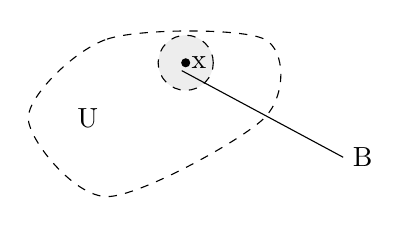
\begin{tikzpicture}
        \draw[dashed] plot [smooth cycle] coordinates {(0,0) (1,1) (3,1) (3,0) (1,-1)};
        \node [right] at (0.5,0) {U};
        \draw[fill=lightgray,dashed] (2,0.7) circle [radius=0.35];
        \draw[fill] (2, 0.7) circle [radius=0.05];
        \node [right] at (1.95,0.7) {x};
        \node [right] at (4,-0.5) {B};
        \draw (1.95,0.6)--(4,-0.5);
        \end{tikzpicture}
      \end{center}

      \item $\T$ consists of all possible unions of elements in $\B$. 
      \begin{equation}
        \T \equiv \Big\{ \bigcup_i B_i \mid B_i \in \B\Big\}
      \end{equation}
    \end{enumerate}
  \end{theorem} 
  \begin{proof}
    We prove that the 2 methods generate a topology, and then finally prove that it they are the same topology. 
    \begin{enumerate}
      \item Clearly, $\emptyset$ and $X$ itself are in $\T$. To prove property 2, given a certain indexed family of subsets $\{U_\alpha\}_{\alpha \in I}$ of $\T$, we must show that 
      \begin{equation}
        U = \bigcup_{\alpha \in I} U_\alpha \in \T
      \end{equation}
      Given $x \in U$, there exists at least one index $\alpha$ such that $x \in U_\alpha$. Since $U_\alpha \in \T$ already, there exists a basis element $b \in \B$ such that $x \in b \subset U_\alpha$. But 
      \begin{equation}
        U_\alpha \subseteq U \implies b \subset U
      \end{equation}
      So, by definition, any arbitrary union of $U$ of these subsets is also in $\T$. 

      To prove property 3, we must show that 
      \begin{equation}
        W = \bigcap_{\alpha \in I} U_\alpha \in \T
      \end{equation}
      Given $x \in W$, by definition of a basis element, there exists a $b \in \B$ such that 
      \begin{equation}
        x \in b \subset (U_\beta \cap U_\gamma) \forall \beta, \gamma \in I \implies \text{ there exists } \Tilde{b} \in \B \text{ s.t. } x \in \Tilde{b} \subset \bigcap_{\alpha \in I} U_\alpha
      \end{equation}
      By definition, $W$ is also open. Since this arbitrary set of subsets $\T$ suffices the 3 properties, it is a topology of $X$ by definition. 

      \item $(\rightarrow)$ Given a collection of elements in $\B$, they are also elements of $\T$. Since $\T$ is a topology, their union in also in $\T$. 

      $(\leftarrow)$ Given an open set $U \in \T$, for every point $x \in U$, by definition we can choose a basis element $b \in \B$ such that $x \in b \subset U$. Then, the union of all these basis elements is by definition $b$. 
        
    \end{enumerate}
  \end{proof}

  We have learned how to go from a basis to a topology. The following lemma tells us how to identify a basis within a topology. 

  \begin{theorem}[Topology to Basis]
    Let $(X, \T)$ be a topological space, and let $\B$ be a collection of open subsets of $X$ such that for every open set $U$ and each $x \in U$, there exists an element $B \in \B$ such that
    \begin{equation}
      x \in B \subset U
    \end{equation}
    Then, $\B$ is a basis for the topology of $X$. 
  \end{theorem}
  \begin{proof}
    Note that there are two claims here: $\B$ is a basis and the topology that $\B$ generates is equal to $\T$. 
    \begin{enumerate}
      \item To prove that $\B$ is a basis, note that $X$ is an open set, and by assumption, for every $x \in X$, there exists a $B \in \B$ s.t. $x \in B \subset X$. Therefore $\B$ covers $X$. Now take two basis elements $B_1, B_2 \in \B$ with $x \in B_1 \cap B_2$. Since we know that $B_1, B_2$ are open, $B_1 \cap B_2$ is open and so for each $x \in B_1 \cap B_2$, there exists a basis element $B_3$ s.t. $x \in B_3 \in (B_1 \cap B_2)$. Thus $\B$ is a basis. 

      \item Let us call $\T^\prime$ the topology generated by $\B$. Then, given $U \in \T$, by assumption for any $x \in U$, there exists a basis element $B \in \B$ s.t. $x \in B \subset U$, so $x \in \T^\prime$. Conversely, if $U \in \T^\prime$, then $U$ is an arbitrary union of elements $B \in \B$ where each $B$ is open in $\T$, so $U \in \T$. So $\T = \T^\prime$. 
    \end{enumerate}
  \end{proof} 

  Characterizing topologies in terms of basis is quite effective since we can work with more manageable sets. 

  \begin{lemma}[Fineness w.r.t. Basis]
    Given two topologies $\T$ and $\T^\prime$ with their bases $\B$ and $\B^\prime$, respectively, the following are equivalent. 
    \begin{enumerate}
      \item $\T^\prime$ is finer than $\T$. 
      \item For each $x \in X$ and basis element $B \in \B$ containing $x$, there exists a basis element $B^\prime \in \B^\prime$ such that $x \in B^\prime \subset B$. 
    \end{enumerate}
  \end{lemma}

  So we have seen how we can take a collection of sets satisfying the basis properties and construct a topology as the union of the sets in this collection. What happens if we can relax some of these conditions? Note that the first condition was that the basis elements must cover $X$. This is non-negotiable. However, if we remove the second requirement that a basis element must be contained in an intersection of basis elements, we can get a \textit{subbasis}. 

  \begin{definition}[Subbasis]
    A \textbf{subbasis} $\mathscr{S}$ for a topology on $X$ is a collection of subsets of $X$ whose union is equal to $X$. 
  \end{definition}

  \begin{theorem}[Subbasis to Topology]
    Given a subbasis $\mathscr{S}$ on a set $X$, the \textbf{topology generated by $\mathscr{S}$} is defined to be the collection $\T$ of all unions of finite intersections of elements of $\mathscr{S}$. 
  \end{theorem}
  \begin{proof}
    It suffices to show that the collection of finite intersections of elements form a basis. 
  \end{proof}
 
\subsection{Limit Points and Closed Sets} 

  First, we need to learn what it generally means for a point to be infinitesimally close to a set. 

  \begin{definition}[Limit Point]
    Given a topological space $(X, \T)$, let $x \in X$ be a point and $S \subset X$ a subset. $x$ is a \textbf{limit point of $S$} if every punctured neighborhood of $x$ intersects $S$.\footnote{Note that limit point are generally used to talk about points that are infinitesimally close to a set $S$. A limit point may not necessarily be in $S$, and a point of $S$ may not necessarily be a limit point. This is why we use a punctured neighborhood, rather than an open neighborhood. For continuity as we will see later, we just talk about neighborhoods since we also claim that the limit exists and the function value is the limit.} The set of all limit points of a set $S$ is denoted $S^\prime$.  
  \end{definition} 

  \begin{example}[Examples of Limit Points]
    What about the limit points that are not in $S$? Generally, there are two instances. 
    \begin{enumerate}
      \item Let $S$ represent the gray area. $B$ is in the ``interior'' of $S$ and therefore is a limit point. $A$ and $C$ are on the ``boundary'' of $S$ yet not in $S$, and we can show that they are limit points as well. 
        
      \begin{figure}[H]
        \centering 
        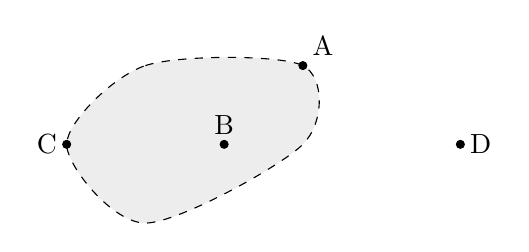
\begin{tikzpicture}
          \draw[fill=lightgray, dashed] plot [smooth cycle] coordinates {(0,0) (1,1) (3,1) (3,0) (1,-1)};
          \draw [fill] (3, 1) circle [radius=0.05];
          \node [above right] at (3,1) {A};
          \draw [fill] (2,0) circle [radius=0.05];
          \node [above] at (2,0) {B};
          \draw [fill] (0,0) circle [radius=0.05];
          \node [left] at (0,0) {C};
          \draw [fill] (5,0) circle [radius=0.05];
          \node [right] at (5, 0) {D};
        \end{tikzpicture}
        \caption{Points $A, B, C$ are limit points of the open set. }
        \label{fig:limit_boundary}
      \end{figure}

      \item A point can be at the ``convergence point'' of a sequence. 
      \begin{figure}[H]
        \centering 
        \begin{tikzpicture}
          \draw [fill] (0, 2.2) circle [radius=0.05];
          \draw [fill] (1, 2.4) circle [radius=0.05];
          \draw [fill] (2, 2) circle [radius=0.05];
          \draw [fill] (2.5, 1.8) circle [radius=0.05];
          \draw [fill] (2.6, 1.6) circle [radius=0.05];
          \draw [fill] (2.65, 1.67) circle [radius=0.05];
          \draw [fill] (2.654, 1.64) circle [radius=0.05];
          \draw [fill] (2.6543, 1.63) circle [radius=0.05];
          \node [right] at (2.6543, 1.63) {p};
        \end{tikzpicture}
        \caption{Note that if $S$ is a sequence of points in $\mathbb{R}^{2}$ that converges to $p$ without ever hitting it, we can say that $p \not\in S$ is a limit point of $S$.}
        \label{fig:limit_sequence}
      \end{figure}
    \end{enumerate}
  \end{example}

  \begin{example}[Examples of Non-Limit Points]
    There are generally two instances of non-limit points. Let $X = \mathbb{R}$ and $S = (0, 1) \cup \{2\}$. 
    \begin{enumerate}
      \item $5$ is clearly not a limit point. 
      \item $2$, although in $S$, is not a limit point since we are talking about the punctured neighborhood. A point in $S$ that is not a limit point is called an \textbf{isolated point}. 
    \end{enumerate}
  \end{example}

  \begin{example}[Counterintuitive Limit Points in Lower Limit Topology]
    Note that given an interval $(a, b) \subset \mathbb{R}$ in the lower limit topology, $a$ is a limit point but $b$ is \textit{not} a limit point!
  \end{example}

  \begin{definition}[Closed Set]
    A set $S \subset X$ is \textbf{closed} if its complement $X \setminus S$ is open in $\T$.\footnote{Note that open and closed sets are not mutually exclusive. A set might be open, closed, both, or neither. A set that is both open and closed is called \textbf{clopen}.}
  \end{definition}
  
  Another property, which is often used as the definition of a closed set, is that it contains all of its limit points. 

  \begin{lemma}[Closed Sets Contain Limit Points]
    A set $S \subset X$ is closed iff it contains all of its limit points. 
  \end{lemma}
  \begin{proof}
    We prove bidirectionally. 
  \end{proof}

  \begin{theorem}[Topological Space wrt Closed Sets]
    Let $X$ be a topological space. Then, the following conditions hold
    \begin{enumerate}
      \item $\emptyset$ and $X$ are clopen.
      \item Arbitrary intersections of closed sets are closed. 
      \item Finite unions of closed sets are closed. 
    \end{enumerate}
  \end{theorem}

  \begin{definition}[Dense Subsets]
    Let $S \subset (X, \tau_X)$. $S$ is \textbf{dense} in $X$ if every point $p \in X$ is a limit point of $S$. In other words, for any point $p \in X$ and any open neighborhood $U_p$ of $p$, $U_p \cap S$ is nontrivial. Otherwise, $p$ is a point of $S$. 
  \end{definition}

  The following example is a crucial fact for proving further properties of topological spaces. 

  \begin{example}
    $\mathbb{Q}^{n}$ is a dense set of $\mathbb{R}^{n}$ with the open ball topology. If we have the discrete topology of $\mathbb{R}^{2}$, an open neighborhood of a point is the point itself, so no limit points would exist beyond the points in $S$ itself. So $\mathbb{Q}^{n}$ is not dense in $\mathbb{R}^{n}$ with this topology. 
  \end{example}

\subsection{Interiors and Closures}

  Now that we've determined limit points, we would like to extend sets into their limit points. The process of doing this is called the \textit{closure} of a set. 

  \begin{definition}[Closure]
    The \textbf{closure} of set $S$ is $\overline{S}$ is defined in the following equivalent ways. 
    \begin{enumerate}
      \item $\overline{S} = S \cup S^\prime$, i.e. the union of itself and its limit points. 
      \item $\overline{S}$ is the intersection of all closed sets $C$ containing $S$. 
    \end{enumerate}
  \end{definition}
  \begin{proof}
    
  \end{proof}

  \begin{example}
    If $S$ is an open ball, $\Bar{S}$ is the closed ball. 
  \end{example}

  From semantics, it may seem like the interior and exterior (defined later) are related, but from a mathematical point of view, the interior and closure are dual notions. 

  \begin{definition}[Interior]
    Let $S \subset X$. Then, the following definitions of the \textbf{interior} of $S$, denoted $S^\circ$, are equivalent. 
    \begin{enumerate}
      \item $x \in S^\circ$ if $\exists U_x \ni x$ s.t. $U_x \subset S$. 
      \item $S^\circ$ is the union of all open sets contained in $S$. 
      \item $S^{o}$ is the complement of the closure of the complement of S. 
      \begin{equation}
        S^{o} = \big(\overline{S^{c}}\big)^{c}
      \end{equation}
    \end{enumerate}
  \end{definition}
  \begin{proof}
    
  \end{proof}

  \begin{lemma}[Open and Closed in Terms of Interiors and Closures]
    Let $S$ be a subset of some topological space $X$. 
    \begin{enumerate}
      \item $S$ is open iff $S = S^{o}$. $S^{o}$ is always open.
      \item $S$ is closed iff $S = \overline{S}$. $\overline{S}$ is always closed. 
    \end{enumerate}
  \end{lemma}

  \begin{theorem}[Clopen sets in Reals]
    There are no proper clopen sets in $\mathbb{R}$. 
  \end{theorem}

\subsection{Exteriors and Boundaries}

  \begin{definition}[Exteriors]
    Let $S \subset X$. The \textbf{exterior} of $S$, denoted $S^e$, is defined in the following equivalent ways.\footnote{We can informally think of the exterior being strictly outside of $S$ and its boundary.}
    \begin{enumerate}
      \item $S^e$ is the complement of the closure of $S$. 
      \item $S^e$ is the interior of the complement of $S$. 
    \end{enumerate}
  \end{definition}
  \begin{proof}
    
  \end{proof}

  \begin{definition}[Boundary]
    Let $S \subset X$. The \textbf{boundary} of $S$, denoted $\partial S$, is defined in the following equivalent ways. 
    \begin{enumerate}
      \item $\partial S$ is the closure minus the interior of $S$ in $X$. 
      \item $\partial S$ is the intersection of the closure of $S$ with the closure of its complement, i.e the set of all points $x$ such that every neighborhood $U_x$ intersects both the interior and exterior. 
      \item $\partial S$ is the set of points that are neither in the exterior nor the interior. 
      \item $x \in \partial S$ if every neighborhood of $x$ intersects both the interior and exterior of $S$. 
    \end{enumerate}
  \end{definition}
  \begin{proof}
    
  \end{proof}

  From the above, we get the intuitive notion that these three parts divide up the whole space. 

  \begin{theorem}[Partitioning of Space]
    Given $S \subset X$, $X$ is partitioned into the interior, boundary, and exterior of $S$. 
    \begin{equation}
      X = S^\circ \sqcup \partial S \sqcup S^e
    \end{equation}
  \end{theorem}
  \begin{proof}
    The fact that 
  \end{proof}

  One counterintuitive result is the \href{https://en.wikipedia.org/wiki/Lakes_of_Wada}{Lakes of Wada}, which are three disjoint connected open sets of the open unit square $(0, 1)^2$ with the property that they \textit{all} have the same boundary. In other words, for any point selected on the boundary of one of the lakes, the other two lakes' boundaries also contain that point. 

 
\section{Common Topologies} 

  We have given some examples of how we can construct topologies from scratch given an arbitrary set $X$, possibly with some structure. Now given a collection of 1 or more topological spaces, we will talk about how we can construct new topologies. Note that the topologies introduced in this section don't really require us to talk about functions yet. They can be constructed and completely described in terms of sets. 

\subsection{Order Topology}

  \begin{definition}[Order Topology]
    \label{def:order-topology}
    Let $X$ be a set with a simple order relation. Let $\B$ be the collection of all sets of the following types.\footnote{If $X$ has no minimum or maximum, then there are no sets of type of 2 or 3, respectively.}
    \begin{enumerate}
      \item All open intervals $(a, b) \coloneqq \{x \in X \mid a < x < b\} \subset X$
      \item All half-open intervals $[a_0, b)$, where $a_0$ is the minimum element of $X$
      \item All half-open intervals $(a, b_0]$, where $b_0$ is the maximum element of $X$. 
    \end{enumerate}
    This set $\B$ is a basis for the \textbf{order topology} of $X$. 
  \end{definition}
  \begin{proof}
    We prove that this set $\mathscr{B}$ is a basis. 
    \begin{enumerate}
      \item It covers $X$. If $x \in X$ is the maximum or minimum we can cover it with $(a, b_0]$ and $[a_0, b)$, respectively. If not, then $x$ is bounded above and below, and so there exists $a, b \in X$ s.t. $a < x < b \implies x \in (a, b)$. 

      \item Let $x \in (a_1, b_1)$ and $x \in (a_2, b_2)$. Then, 
      \begin{equation}
        x \in (\max\{a_1, a_2\}, \min\{b_1, b_2\}) \in \mathscr{B} 
      \end{equation}
    \end{enumerate}
    Therefore, the generated collection is indeed a topology. 
  \end{proof}

  \begin{example}[Standard Order Topology on $\mathbb{R}$]
    The standard topology on $\mathbb{R}$ is precisely the order topology derived from the usual order on $\mathbb{R}$. Since $\mathbb{R}$ has no minimum or maximum, the basis consists of open intervals $(a, b) \subset \mathbb{R}$ with $a, b \in \mathbb{R}$. 
  \end{example}

  \begin{example}[Basis of Open Intervals with Rational Endpoints]
    We can however get away with smaller basis that generate the same topology on $\mathbb{R}$. If we take the set of all open intervals $(a, b) \subset \mathbb{R}$ with $a, b \in \mathbb{Q}$, this is also a basis for the same standard order topology. Too see why, let us denote this basis as $\B^\prime$ and the basis of all open intervals with real endpoints be $\B$. Then, clearly $B^\prime \subset \B \implies \T^\prime \subset \T$. As for the other, way, let us take an open interval $(a, b) \in \B$. Then we can see that 
    \begin{equation}
      (a, b) = \bigcup_{\substack{p, q \in \mathbb{Q} \\ a < p, q < b}} (p, q)
    \end{equation}
    where equality follows from density of rationals in $\mathbb{R}$. 
  \end{example}

  \begin{example}[$\mathbb{R}^2$ with Dictionary Order]
    Given $\mathbb{R} \times \mathbb{R}$ with the dictionary order, then $\mathbb{R} \times \mathbb{R}$ has neither a largest nor smallest element. Therefore, the order topology on $\mathbb{R} \times \mathbb{R}$ consists of all "intervals" of form
    \begin{equation}
      \big((a, b), (c, d) \big) \equiv  \{(x, y) \in \mathbb{R}^2 \mid (a, b) < (x, y) < (c, d)\}
    \end{equation}

    \begin{figure}[H]
      \centering 
      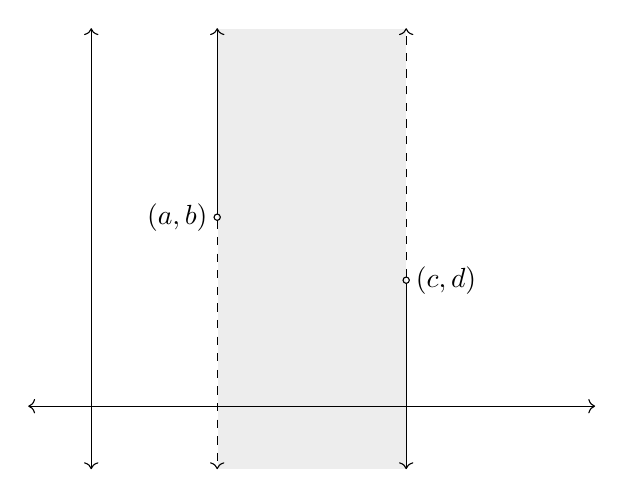
\begin{tikzpicture}[scale=0.8]
        \draw[white, fill=lightgray] (2,-1) rectangle (5,6);
        \draw[<->] (-1,0)--(8,0);
        \draw[<->] (0,-1)--(0,6);
        \draw[->] (2,3.05)--(2,6);
        \draw[->] (5,1.95)--(5,-1);
        \draw (2,3) circle [radius=0.05];
        \draw (5,2) circle [radius=0.05];
        \draw[dashed, ->] (2,2.95)--(2,-1);
        \draw[dashed,->] (5,2.05)--(5,6);
        \node[left] at (2,3) {$(a, b)$};
        \node[right] at (5,2) {$(c,d)$};
      \end{tikzpicture}
      \caption{This means that open rays and lines are also a part of the topology of $\mathbb{R} \times \mathbb{R}$. } 
      \label{fig:r2_dict_order}
    \end{figure}
  \end{example}

  \begin{example}[Positive Integers]
    The set of positive integers $\mathbb{Z}_+$ form an ordered set with a smallest element. The order topology for $\mathbb{Z}_+$ is precisely the discrete topology since every one-point set is an open set. 
    \begin{equation}
      \{n\} = (n-1, n+1)
    \end{equation}
  \end{example}

  \begin{example}[Two Copies of Positive Integers]
    The dictionary order topology on $\{1, 2\} \times \mathbb{Z}_+$ results in every one point set being open, except for the point $(2, 1)$. Since every neighborhood of $(2,1)$ must contain some point of form $(1, n)$ for arbitrarily large $n$, $\{(2,1)\}$ is not open. 
  \end{example}

  \begin{definition}
    If $X$ is an ordered set a $a \in X$, then there are 4 subsets of $X$ called rays determined by $a$. 
    \begin{enumerate}
      \item $(a, +\infty)$ 
      \item $(-\infty, a)$
      \item $[a, +\infty)$
      \item $(-\infty, a]$
    \end{enumerate}
    The first two sets are called \textbf{open rays}, and the latter two sets are called \textbf{closed rays}. 
  \end{definition}

  We can extend the basis of open intervals to some other basis based on the order, which generates other topologies. 

  \begin{example}[Lower/Upper Limit Topology]
    Given a totally ordered set $(X, \leq)$, 
    \begin{enumerate}
      \item the \textbf{lower limit topology} is the topology generated by the basis of all half-closed half-open intervals of form 
      \begin{equation}
        [a, b) \coloneqq \{ x \in X \mid a \leq x < b \}
      \end{equation}
      \item the \textbf{upper limit topology} is the topology generated by the basis of all half-open half-closed intervals of form 
      \begin{equation}
        (a, b] \coloneqq \{ x \in X \mid a < x \leq b \}
      \end{equation}
    \end{enumerate}
  \end{example}

  \begin{example}[Nested Interval Topology]
    In the space $X = (0,1)$, the \textbf{nested interval topology} is the topology generated by the basis of nested intervals of the form 
    \begin{equation}
      \B_{ni} \coloneqq \{ (0, 1-\frac{1}{n}) \mid n \in \mathbb{N} \}
    \end{equation}
  \end{example}

  A topology generated by closed intervals can also be a topology! 

  \begin{example}[Closed Interval Topology]
    In the set $X = [-1, 1]$, the following set 
    \begin{equation}
      \B_{ci} \coloneqq \{ [-1, a) \mid a > 0 \big\} \bigcup \big\{ (b, 1] \mid b<0 \}
    \end{equation}
    is a basis. The topology it generates is called the \textbf{closed interval topology}, denoted $\T_{ci}$. 
  \end{example}

  Finally, we talk about a seemingly arbitrary topology called the K-topology, but it is useful for counterexamples.   

  \begin{example}[K-Topology]
    In $\mathbb{R}$, let us denote $K = \{1/n\}_{n \in \mathbb{N}}$. Then the \textbf{K-topology} on $\mathbb{R}$ is the topology generated by the basis consisting of 
    \begin{enumerate}
      \item all open intervals $(a, b)$ with $a, b \in \mathbb{R}$. 
      \item all sets of the form $(a, b) \setminus K$ with $a, b \in \mathbb{R}$. 
    \end{enumerate}
  \end{example} 

  Now that we have some collection of topologies, let's try to compare them. We claim the following. 

  \begin{theorem}[Comparison of Topologies of the Real Line]
    
  \end{theorem}

\subsection{Metric Topology}

  For common sets like $\mathbb{R}^n$, which has an inner product, or $\mathbb{Q}$, which has an order, it is easy to build these topologies with set-builder notation. Consider the following. 

  \begin{definition}[Metric Topology]
    \label{def:metric-topology}
    Given a metric space $(X, d)$, let us denote the \textbf{metric topology}, or \textbf{open-ball topology}, as the set of subsets $U$ satisfying the property that for all $x \in U$, there exists a positive $r \in \mathbb{R}$ such that $B(x, r) \subset U$, where $B(x, r) \coloneqq \{y \in X \mid d(x, y) < r\}$ is the open ball of radius $r$ around $x$. We claim that this is a topology. 
  \end{definition} 
  \begin{proof}
    We show that the properties of a topology hold. 
    \begin{enumerate} 
      \item For the empty set, the inclusion of an open ball for a point in $\emptyset$ is vacuously satisfied. For the whole set, we choose any point $x$ and any $r$, and the open ball is trivially a subset of $X$. 

      \item Let $\{U_\alpha\}_{\alpha \in I}$ be a collection of open subsets of $X$. Let their union be denoted $U$. We claim $U$ is open. Pick any point $x \in U$. Then by definition of union, there exists some $\alpha \in I$ s.t. $x \in U_\alpha$. Since $U_\alpha$ is open, there exists a $r > 0$ s.t. $B(x, r) \subset U_\alpha \subset U$. Therefore $U$ is open. 

      \item Let $U_1, \ldots, U_k$ be open, and let us denote their intersection as $U$. We claim $U$ is open. Pick a point $x \in U$. Then for each $i = 1, \ldots, k$, $x \in U_i$ and there exists a corresponding $r_i > 0$  such that the open ball $B(x, r_i) \subset U_i$. Take the set $R = \{r_i\}$, which is a finite set living in $\mathbb{R}$. We will take for granted that every finite subset of an ordered set has a minimum.\footnote{If we wish to prove it, we can start with a singleton set, claim that its minimum is the only element. Then we use induction by assuming for a set $R$ of size $k$ that a minimum exists, and by adding $1$ more element $r$ we update the minimum to be $\min\{r, \min{R}\}$ and show that this is indeed the minimum.} Let us denote $r^\ast = \min{R}$, and we claim that $r^\ast$ gives us a ball that can fit inside $U$. Assume $y \in B(x, r^\ast)$. Then 
      \begin{align}
        y \in B(x, r^\ast) & \implies d(x, y) < r^\ast \\ 
                           & \implies d(x, y) < \min{R} \\
                           & \implies d(x, y) < r_i \text{ for } i = 1, \ldots, k \\
                           & \implies y \in B(x, r_i) \text{ for } i = 1, \ldots, k
      \end{align} 
      Since $B(x, r_i)$ by construction is contained within $U_i$, $y \in U_i$ for all $i$. This means by definition of intersection that $y \in U$, and we have proven that $B(x, r^\ast)$ completely fits inside $U$. 
    \end{enumerate}
  \end{proof} 

  Note that while open balls are used to define whether a set is open or not, the definition doesn't state whether open balls themselves are open sets. It turns out that it is easy to prove that they are. 
  
  \begin{lemma}[Open Balls are Open Sets]
    The open ball wrt any metric $d$ is an open set wrt the metric topology. 
  \end{lemma}
  \begin{proof}
    Let $y \in B(x, r)$. Then $d(x, y) < r \implies 0 < r - d(x, y)$. To show that $B(x, r)$ is open, we would like to show that there exists some $r^\prime > 0$ s.t. $y \in B(y, r^\prime) \subset B(x, r)$. Set $r^\prime = r - d(x, y)$. Then 
    \begin{align}
      z \in B(y, r^\prime) & \implies d(y, z) < r - d(x, y) \\
                           & \implies d(x, y) + d(x, y) < r \\
                           & \implies d(x, z) < r \\
                           & \implies z \in B(x, r)
    \end{align} 
    and so $B(y, r^\prime) \subset B(x, r)$. We are done. 
  \end{proof}

  \begin{example}[Discrete Metric Induces Discrete Topology]
    Given a set $X$, induce the metric $d$ defined
    \begin{equation}
      d(x, y) \equiv \begin{cases} 1 & \text{if } x \neq y \\ 0 & \text{if } x = y \end{cases}
    \end{equation}
    This metric induces the discrete topology on $X$, since the basis elements of the open balls
    \begin{equation}
      B_r (x) \equiv \{ y \in X \mid d(x, y) <r\}
    \end{equation}
    consists of two types of open sets. When $r \leq 1$, then $B_r (x) = x$ (since the radius is $0$). If $r > 1$, then the open set is the entire space $X$. 
  \end{example} 

  While the behavior for finite sets are predictable under the metric topology, as soon we we get into infinite sets, the properties of the metric topology may differ. 

  \begin{example}[Metric Topologies on $\mathbb{Z}$ and $\mathbb{Q}$]
    $\mathbb{Z}$ and $\mathbb{Q}$ are countable sets, so there is a bijection between them. If we give each of them the metric topology, $\mathbb{Z}$ ends up having the discrete topology (take the $0.5$-ball around each integer), whereas for $\mathbb{Q}$, we will see later that by the density of the rationals there are an infinite number of rationals in $(q - r, q + r)$ for $q \in \mathbb{Q}$. Therefore, the metric topology may or may not induce the discrete topology. 
  \end{example}

  \begin{example}[Supremum Norm in $\mathbb{R}^3$]
    \begin{figure}[H]
      \centering 
      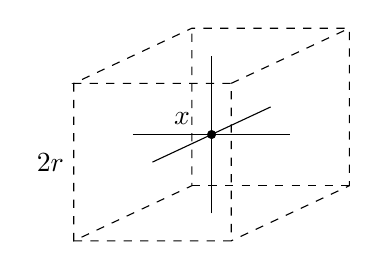
\begin{tikzpicture}
        \draw[dashed] (0,0)--(2,0)--(2,2)--(0,2)--(1.5,2.7)--(3.5,2.7)--(3.5,0.7)--(2,0);
        \draw[dashed] (2,2)--(3.5,2.7);
        \draw[dashed] (0,2)--(0,0)--(1.5,0.7)--(1.5,2.7);
        \draw[dashed] (1.5,0.7)--(3.5,0.7);
        \draw (1,1)--(2.5,1.7);
        \draw (0.75,1.35)--(2.75,1.35);
        \draw (1.75,0.35)--(1.75,2.35);
        \draw[fill] (1.75,1.35) circle (0.05);
        \node[above left] at (1.6,1.35) {$x$};
        \node[left] at (0,1) {$2r$};
      \end{tikzpicture}
      \caption{In $\mathbb{R}^3$, each basis element is a cube centered at $x$ with side lengths $2r$.} 
      \label{fig:}
    \end{figure}
  \end{example}

  \begin{theorem}[Metric Topologies on Finite Sets]
    If $(X, d)$ is a finite metric space, then the metric topology on it is the discrete topology. 
  \end{theorem}
  \begin{proof}
    Take all pairwise points and compute $\epsilon = \min_{x \neq y} \{d(x, y)\}$. Since $X$ is finite, all pairs are finite and therefore the minimum exists. Now let us take the $\epsilon$-ball around $x$. Then every $y \neq x$ has distance $d(x, y) \geq \epsilon$, and therefore $y \not\in B(x, \epsilon)$. So all single points are open sets, which induces the discrete topology. 
  \end{proof}

  A finite set $S$ of points does not have any limit points, since if we draw small enough circles around a $p \in S$, then at some point the circle will not contain any more points (remember that we're talking about deleted neighborhoods). Following this, we can deduce that a limit point must always have an infinite number of points close to it, as in no matter how small the circle gets, there are always an infinite number of points contained within that circle. This also means that if $p$ is a limit point, then we can construct a sequence of points in $S$ that converges to $p$, since every open ball with smaller and smaller radii will still have points in $S$.

  \begin{theorem}[Neighborhood of Limit Point Contains Infinite Points in Metric Space]
    Let $X$ be a metric space. If $p$ is a limit point of $S$, then every neighborhood of $p$ contains infinitely many points of $S$. The converse is also true trivially. 
  \end{theorem}
  \begin{proof}
    Assume $p$ is a limit point and that there exists a finite number of points within a deleted neighborhood $B_r^\circ (p)$. Then, we can enumerate them $p_1, p_2, \ldots, p_n$ by their distances to $p$, with 
    \begin{equation}
      d(p_1, p) \leq d(p_2, p) \leq \ldots \leq d(p_n, p)
    \end{equation}
    Since $p_1 \neq p$, we have $d(p_1, p) > 0$ and so, we can choose an $0 < \epsilon < d(p_1, p)$ s.t. $B_\epsilon^\circ (p)$ does not contain any of the $p_i$'s. This neighborhood does not contain any elements of $S$ and so $p$ is not a limit point. 
  \end{proof}

  \begin{corollary}[Finite Set in Metric Space has No Limit Points]
    Let $X$ be a metric space and $S = \{s_i\}_{i=1}^n$ be a finite set. Then, $S^\prime = \emptyset$.  
  \end{corollary}
  \begin{proof}
    If $S$ is a finite set, then every neighborhood of every point $p$ in $\mathbb{R}^n$ will have at most finite points, which, by the previous theorem, is not a limit point. 
  \end{proof}


  It is easy to go from a metric to a topology, but a natural question is that given a topology, does there exist a metric that induces this topology? This is precisely the notion of \textit{metrizability}, which is a highly desirable attribute for spaces, and there are many existence theorems that proves metrizability given certain conditions.

  \begin{definition}[Metrizable Space]
    If $(X, \T)$ is a topological space, $(X, \T)$ is said to be \textbf{metrizable} if there exists a metric $d$ on $X$ that induces the topology $\T$ of $X$.
  \end{definition}

  \begin{example}[Non-Metrizable Finite Spaces]
    Let $X = \{a, b c\}$. Then the topology 
    \begin{equation}
      \T = \{\emptyset, \{b\}, \{a, b\}, \{b, c\}, X \}
    \end{equation} 
    is not metrizable from the theorem above since the only metrizable topologies are discrete. 
  \end{example}

  \begin{lemma}[Fineness of Metric Topologies]
    Let $d$ and $d^\prime$ be two metrics on the set $X$ with their respective induced topologies $\T, \T^\prime$. We claim that $\T \subset \T^\prime$ iff there exists a $M > 0$ s.t. 
    \begin{equation}
      d^\prime (x, y) < M \cdot d(x, y)
    \end{equation} 
    for all $x, y \in X$. That is, we can bound $d^\prime$ with a constant multiple of $d$. 
  \end{lemma}
  \begin{proof}
    
  \end{proof}

\subsection{Euclidean Topology}

  More specifically, the metric topology generated by the $L_2$-metric on $\mathbb{R}^n$ is called the \textbf{Euclidean topology}. Note that the topological property of stability under countable intersection was required to show that the minimum of $R$ existed. This is not true for infinite sets in general. This gives us some motivation as to why we need the \textit{finite} intersection rather than an infinite one. 
  
  \begin{lemma}[Singletons are Not Open in $\mathbb{R}^n$]
    A singleton set is not open in $\mathbb{R}^n$ with the Euclidean topology.   
  \end{lemma}
  \begin{proof}
    We claim that the singleton set $S = \{0\}$ is not open under the Euclidean metric. We pick a point in $S$, which can only be $0$. Assume that there exists an $r > 0$ s.t. $B(x, r) \subset S$. $\mathbb{R}$ is Archimedean, so there exists a natural number $N$ s.t. $0 < 1/N < r$. We construct the vector $v = (v_1, \ldots, v_n)$ s.t. $v_1 = 1/N$ and $v_i = 0$ everywhere else. The distance between $0$ and $v$ is 
    \begin{equation}
      \| v - 0 \| = \|v\| = \sqrt{(1/N)^2} = 1/N < r
    \end{equation} 
    so $v \in B(x, r)$. But $v \neq 0$, and by contradiction such an $r$ cannot exist. In $\mathbb{R}^n$ we consider the countable intersection of open balls (which we have proved in class are open sets) around $0$ of radius $1/N$ for $n \in \mathbb{N}$. We claim that 
    \begin{equation}
      \bigcap_{n \in \mathbb{N}} B(0, 1/n) = \{0\}
    \end{equation} 
    We see that $1/n$ must always be positive and so $\|0 - 0\| = 0 < 1/n$. Therefore the LHS $\supset $ RHS. To see that the intersection contains no other element, consider any vector $v \neq 0$. Then by definition of the metric, $d(v, 0) > 0$. By the Archimedean property, there exists a natural $N \in \mathbb{N}$ s.t. $0 < 1/N < d(v, 0)$, which means that $v \not\in B(0, 1/N)$, and so $v$ cannot be in the intersection. Therefore, the intersection must be $\{0\}$, and we have shown that $B_0$ is not open, so we are done. 
  \end{proof}

  \begin{theorem}
    For a metric space $(X, d)$, the metric topology is finer than the cofinite topology. 
  \end{theorem} 
  \begin{proof}
    Note that if $X$ is finite, then both are reduced to the discrete topologies. 
  \end{proof}

  While it is not surprising that a basis uniquely generates a topology, it is not immediately obvious \textit{what} the generated topology looks like. It turns out that many different bases may generate the same topology, and the concept of fineness allows us to compare these topologies more effectively. For example, if two topologies are both finer than the other, then they must be equal. 

  \begin{theorem}[Euclidean Topology on $\mathbb{R}^n$]
    \label{thm:lp-norms-euclidean-topology}
    $L^p$ norms all generate the same topology on $\mathbb{R}^n$. 
  \end{theorem}
  \begin{proof}
    We can show that 
    \begin{equation}
      n^q d_\infty \leq n^q d_2 \leq n^q d_1 \leq d_p \leq n^{-p} d_\infty
    \end{equation}
    where $q$ is the holder conjugate of $p$. Visually, we can see that every open ball in $(\mathbb{R}^n, d)$ (with the Euclidean metric) is the form to the left, while an open ball in $(\mathbb{R}^n, \rho)$ (with the square metric) is of form on the right. 
    \begin{center}
      \begin{tikzpicture}[scale=0.5]
        \draw [dashed] (1,0) circle [radius=2];
        \draw [dashed] (6,-2) rectangle (10,2);
        \draw [fill] (1,0) circle [radius=0.05];
        \node [above left] at (1,0) {x};
        \draw (1,0)--(3,0);
        \node [above] at (1.5,0) {r};
        \draw [fill] (8,0) circle [radius=0.05];
        \node [below right] at (8,0) {x};
        \draw (8,0)--(10,0);
        \draw (8,0)--(8,2);
        \node [right] at (8,1) {r};
        \node [above] at (9,0) {r};
      \end{tikzpicture}
    \end{center}
    Clearly, we can form any open set of any "shape" using any arbitrary combination of these "circles" or "squares," indicating that they generate the same topology. 
  \end{proof}

\subsection{Cofinite Topology}

  \begin{definition}[Cofinite Topology]
    Given a set $X$, the set of all subsets $U$, satisfying the property that $X \setminus U$ is finite, is a topology, called the \textbf{cofinite topology} or the \textbf{finite complement topology}.\footnote{While this definition may seem a bit arbitrary, this is very similar to the Zariski topology, which is used in algebraic topology.} 
  \end{definition}
  \begin{proof}
    Let us denote this set $\T_c$. 
    \begin{enumerate}
      \item By definition $\emptyset \in \T_c$. It is clear that $X \setminus X = \emptyset$ has cardinality $0$, and therefore is in $\T_c$. 

      \item Let $\{U_\alpha\}_{\alpha \in I} \in \mathcal{T}_c$ by a collection of open sets of $X$. Then by deMorgan's laws, 
      \begin{equation}
        X \setminus \bigcup_{\alpha \in I} U_{\alpha} = \bigcap_{\alpha \in I} (X \setminus U_\alpha)
      \end{equation}
      $X \setminus U_\alpha$ is countable for all $\alpha \in I$, so let us fix some $\alpha^\prime$. Then 
      \begin{equation}
        \bigcap_{\alpha \in I} (X \setminus U_\alpha) \subset U_{\alpha^\prime} \implies \bigg| \bigcap_{\alpha \in I} (X \setminus U_\alpha) \bigg| \leq \big| U_{\alpha^\prime} \big| 
      \end{equation}
      and so the intersection is also countable. 

      \item Let $\{U_i\}_{i=1}^n$ by a finite collection of open sets of $X$. Then by deMorgan's laws, 
      \begin{equation}
        X \setminus \bigcap_{i=1}^n U_i = \bigcup_{i=1}^n (X \setminus U_i)
      \end{equation}
      Since $U_i$ are open, $X \setminus U_i$ are countable, and since the finite union of countable sets are countable, the RHS is countable, which implies the LHS is countable and so $\cap_{i=1}^n U_i$ is open as well. 
    \end{enumerate}
  \end{proof} 

  Slightly modifying the definition does not result in a topology. 

  \begin{example}[Countable Complement is Not A Topology]
    Given a set $X$, consider the collection 
    \begin{equation}
      \T_\infty \coloneqq \{U \subset X \mid X \setminus U \text{ is infinite or empty or all of }X \}
    \end{equation}
    This is not a topology. Let us take $X = \mathbb{R}$, and look at the sets $\mathbb{Z}_{\geq 0}, \mathbb{Z}_{\leq 0}$ consisting of all the non-negative and non-positive integers. They are both infinite, and so $\mathbb{R} \setminus \mathbb{Z}_{\geq 0}$ and $\mathbb{R} \setminus \mathbb{Z}_{\leq 0}$ are in $\mathcal{T}_\infty$. Consider their union. 
    \begin{equation}
      (\mathbb{R} \setminus \mathbb{Z}_{\geq 0}) \cup (\mathbb{R} \setminus \mathbb{Z}_{\leq 0}) = \mathbb{R} \setminus (\mathbb{Z}_{\geq 0} \cap \mathbb{Z}_{\leq 0}) = \mathbb{R} \setminus \{0\}
    \end{equation}
    But $\mathbb{R} \setminus (\mathbb{R} \setminus \{0\}) = \{0\}$, and so $\mathbb{R} \setminus \{0\}$ is not open. Therefore $\mathcal{T}_c$ doesn't satisfy the definition of a topology. 
  \end{example}


\section{Continuity} 

  \subsection{Sequences}

  \subsection{Continuous Functions}

    \begin{definition}[Continuous Function]
      A function $f$ between 2 topological spaces $(X, \mathscr{T}_{X})$ and $(Y, \mathscr{T}_{Y})$ is \textbf{continuous at $x \in X$} if the preimage of every open neighborhood of $f(x) \in Y$ is an open neighborhood of $x \in X$.
      \begin{equation}
        U_{f(x)} \in \mathscr{T}_{Y} \implies x \in f^{-1}(U_{f(x)}) \in \mathscr{T}_{X}
      \end{equation} 
      $f$ is said to be \textbf{continuous} (at all points) if the preimage of every open set in $Y$ is an open set in $X$.\footnote{Note that continuity of a function $f$ is not only determined by the function itself, but also by the topologies of $X$ and $Y$.}
    \end{definition}

    Note that to check if $f$ is continuous, it suffices to check that the preimage of every basis element of the topology of $Y$ under $f$ is open in $X$, since every open set in $Y$ can be constructed as the union of basis elements. More rigorously, an arbitrary open set $V$ of $Y$ can be written as 
    \begin{equation}
      V = \bigcup_{\alpha \in J} b_\alpha
    \end{equation}
    Then, 
    \begin{equation}
      f^{-1} (V) = f^{-1} \Big( \bigcup_{\alpha \in J} b_\alpha \Big) = \bigcup_{\alpha \in J} f^{-1} (b_\alpha)
    \end{equation}

    \begin{theorem}[Sufficient Properties for Continuity]
      Let $X, Y$, be topological spaces and let $f: X \longrightarrow Y$. Then, the following are equivalent. 
      \begin{enumerate}
        \item $f$ is continuous. 
        \item For every subset $A$ of $X$, $f(\bar{A}) \subset \bar{f(A)}$. 
        \item For every closed set $B$ in $Y$, the set $f^{-1} (B)$ is closed in $X$. 
      \end{enumerate}
    \end{theorem}  

    \begin{theorem}[Continuous Bijections]
      Suppose $f$ is bijective. Then 
      \begin{enumerate}
        \item $f$ is continuous implies for every open $U \subset Y$, $f^{-1} (U)$ is open in $X$. 
        \item $f^{-1}$ is continuous implies for every open $U \subset X$, $(f^{-1})^{-1} (U) = f(U)$ is open in $Y$.\footnote{Note by overloading the $-1$ exponent operator, the inverse and preimages are confusing. The inner represents the inverse and the outer represents the preimage. }
      \end{enumerate}
    \end{theorem} 

    \begin{theorem}[Analytic Continuity = Topological Continuity] 
      Given metric spaces with their induced metric topologies $(X, \mathscr{T}_X, d_X)$ and $(Y, \mathscr{T}_Y, d_Y)$. The following are equivalent. 
      \begin{enumerate}
        \item $f: X \rightarrow Y$ is continuous at $x$. 
        \item For every $\delta > 0$, there exists an $\epsilon = \epsilon(\delta) > 0$ such that for all $z \in X$, $d_X (x, z) < \epsilon \implies d_Y (f(x), f(x)) < \delta$.\footnote{This is the definition of continuity at a point in analysis.} 
      \end{enumerate}
    \end{theorem}
    \begin{proof}
      
    \end{proof}

  \subsection{Homeomorphisms}

    \begin{definition}[Homeomorphism]
      A bijective, bicontinuous function 
      \begin{equation}
        f: X \longrightarrow Y
      \end{equation}
      between two topological spaces is called a \textbf{homeomorphism} between $X$ and $Y$. If there exists at least one homeomorphism between $X$ and $Y$, then $X$ is said to be \textbf{homeomorphic} to $Y$. 

      \begin{figure}[H]
        \centering 
        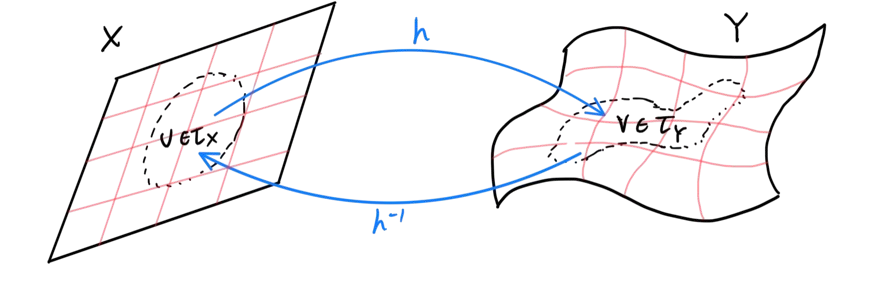
\includegraphics[scale=0.25]{img/Homeomorphism_of_Plane.PNG}
        \caption{The visual below shows a homeomorphism between the plane $X$ and the surface $Y$.}
        \label{fig:homeomorphism_plane}
      \end{figure}
    \end{definition}

    \begin{theorem}[Sufficient Properties of Homeomorphism]
      Suppose $f: X \rightarrow Y$ is a bijection. TFAE. 
      \begin{enumerate}
        \item $U \subset Y$ is open iff $f^{-1} (U)$ is open. 
        \item $U \subset X$ is open iff $f(U)$ is open. 
        \item $f$ is a homeomorphism. 
      \end{enumerate}
    \end{theorem} 

    \begin{example}[Comparability and Homeomorphic Spaces]
      Consider the set $X = \{a, b\}$ with the two topologies $\T_3 = \{\emptyset, \{a\}, X\}$ and $\T_4 = \{\emptyset, \{b\}, X\}$. They are not comparable but they seem ``similar'' in a way in that if we swap all the $a$'s and $b$'s in $\T_3$, then we get $\T_4$. We can make this rigorous by defining $f: (X, \T_3) \rightarrow (X, \T_4)$ with $f(a) = b, f(b) = a$, and showing that it is a homeomorphism. 
    \end{example}

    In fact, a homeomorphism $f$ is an equivalence relation between two topological spaces. This partitions the set of all topological spaces into \textbf{homeomorphism classes}. Analogous to how isomorphisms preserve algebraic structures, homeomorphisms preserve topological structure between topological spaces. 

    Additionally, not only does a homeomorphism give a bijective correspondence between points in $X$ and $Y$, but it also determines a bijection between \textbf{the set of all open sets in $X$ and $Y$} (that is, a bijection between their topologies)! This bijection then allows two spaces that are homeormophic to have the same topological properties. 

    \begin{proposition}
      A homeomorphism $f$ between two topological spaces $(X, \tau_{x})$ and $(Y, \tau_{Y})$ preserves all topological properties (e.g. separability, countability, compactness, (path) connectedness) of $X$ onto $Y$ and $Y$ onto $X$. 
    \end{proposition}

    \begin{definition}
      Suppose that $f: X \longrightarrow Y$ an injective continuous map with $X, Y$ topological spaces. Let $Z \equiv \im{f}$. Then, the function
      \begin{equation}
        f^\prime: X \longrightarrow Z \subset Y
      \end{equation}
      obtained by restricting the codomain of $f$ is bijective. If $f^\prime$ happens to be a homeomorphism of $X$ with $Z$, then we say that the map
      \begin{equation}
        f: X \longrightarrow Y
      \end{equation}
      is a \textbf{topological embedding}, or more simply an \textbf{embedding}, of $X$ in $Y$. 
    \end{definition}

    \begin{lemma}[Pasting Lemma, Gluing Lemma]
      Let $X = A \cup B$, where $A, B$ are closed in $X$. Let $f: A \longrightarrow Y$ and $g: B \longrightarrow Y$ be continuous. If 
      \begin{equation}
        f(x) = g(x) \text{ for all } x \in A \cap B
      \end{equation}
      Then $f$ and $g$ can be combined to form a continuous function $h: X \longrightarrow Y$, defined
      \begin{equation}
        h(x) \equiv \begin{cases}
          f(x) & x \in A \setminus B \\
          f(x) \text{ or } g(x) & x \in A \cap B \\
          g(x) & x \in B \setminus A
        \end{cases}
      \end{equation}
      This is shown in the following visual. 
      \begin{center}
          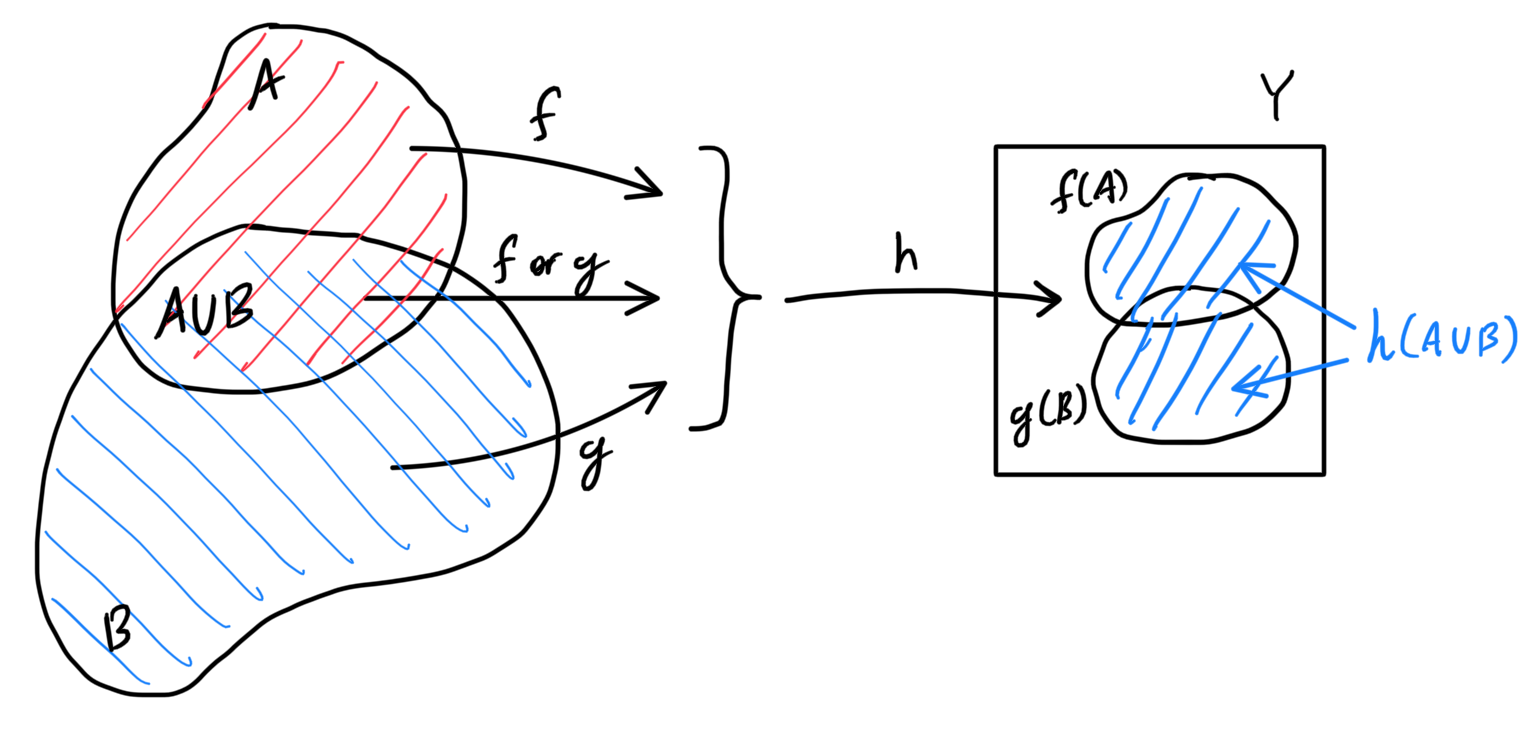
\includegraphics[scale=0.25]{img/Gluing_Lemma.PNG}
      \end{center}
    \end{lemma}

    \begin{theorem}
      Let $f: A \longrightarrow X \times Y$ be given by the equation 
      \begin{equation}
        f(a) \equiv \big( f_1 (a), f_2(a) \big)
      \end{equation}
      Then $f$ is continuous if and only if the function $f_1: A \longrightarrow X$ and $f_2: A \longrightarrow Y$ are continuous. 
    \end{theorem}

    However, there is no useful criterion for the continuity of a mapping 
    \begin{equation}
      f: X \times Y \longrightarrow A
    \end{equation}
    if the domain of $f$ is a product space. One might conjecture that this $f$ is continuous if it is continuous in each variable separately, but this is in fact not true. 


\section{Induced Topologies} 

\subsection{Initial and Final Topologies} 

  We have seen some examples of how to create topologies. They can be created without any assumptions on the set, such as the discrete, indiscrete, and the cofinite topologies. More often, we want to consider how a certain structure like the order or a metric induces a topology. Now, we will consider how \textit{functions} can induce a topology. The uniqueness of such induced topologies is called the \textit{universal property}. 

  \begin{definition}[Initial Topology]
    Given a space $X$ and a family of topological spaces $\{Y_\alpha\}_{\alpha \in A}$ 
    \begin{equation}
      f_i : X \rightarrow (Y_\alpha, \T_\alpha)
    \end{equation} 
    the \textbf{initial topology} on $X$ is the coarsest topology $\T$ on $X$ s.t. that each 
    \begin{equation}
      f_i (X, \T) \rightarrow (Y_\alpha, \T_\alpha)
    \end{equation}
    is continuous. 
  \end{definition}

  \begin{definition}[Final Topology]
    Given a space $Y$ and a family of topological spaces $\{X_\alpha\}_{\alpha \in A}$ 
    \begin{equation}
      f: (X, \T_\alpha) \rightarrow Y
    \end{equation}
    the \textbf{final topology} on $Y$ is the finest topology $\T$ on $Y$ s.t. each 
    \begin{equation}
      f: (X, \T_\alpha) \rightarrow (Y, \T)
    \end{equation}
    is continuous. 
  \end{definition}

  Note that it makes sense to talk about the coarsest topology on the domain and the finest topology on the codomain. If it were the other way around, i.e. the finest topology on the domain, then the initial topology on $X$ would be the discrete topology, making every function defined on $X$ continuous. In the same logic, the coarsest topology on $Y$ would trivially be the trivial topology, making all $Y$-valued functions continuous. With these current definitions, if $\T_Y$ is too fine (e.g. if $\T_Y = 2^Y$), then the open sets of $\T_Y$ would be too fine and therefore would have a preimage that may not be open in $X$. 

\subsection{Subspace Topology} 

  The reason we want to do this is because we want to think of $Y$ as its own entity, independent of $X$. 

  \begin{definition}[Subspace Topology]
    Given topological space $X$ and subspace $Y \subset X$, the \textbf{subspace topology} on $Y$ is defined in the equivalent ways. 
    \begin{enumerate}
      \item It is the initial topology on the subspace $Y$ with respect to the inclusion map $\iota: Y \rightarrow X$. 
      \item It is the topology consisting of $X$-open sets intersection $Y$. 
      \begin{equation}
        \T_Y = \{(U \cap Y) \subset Y \mid U \in \T_X\}
      \end{equation}
    \end{enumerate}

    \begin{figure}[H]
      \centering
      \begin{subfigure}[b]{0.48\textwidth}
        \centering
        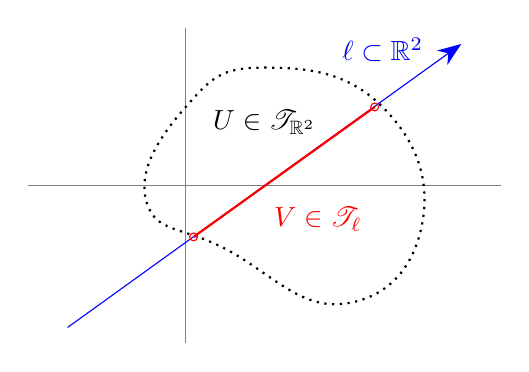
\begin{tikzpicture}
          % Draw the x and y axes in gray
          \draw[gray] (-3,0) -- (3,0);
          \draw[gray] (-1,-2) -- (-1,2);
          
          % Draw a blob (open set) with dotted borders
          \draw[dotted, thick] plot [smooth cycle, tension=0.8] coordinates {(-1,1) (0,1.5) (1.5,1) (2,-0.5) (1,-1.5) (-0.5,-0.8) (-1.5,-0.2)};
          
          % Label the open set
          \node at (0.0,0.8) {$U \in \mathscr{T}_{\mathbb{R}^2}$};
          
          % Draw a straight line passing through the blob with arrows on both ends
          \draw[-{Stealth[length=3mm]}, blue] (-2.5,-1.8) -- (2.5,1.8);
          
          % Label the line
          \node[anchor=north, blue] at (1.5,2) {$\ell \subset \mathbb{R}^2$};
          
          % Bold the portion where the line intersects the blob
          % Calculate or estimate intersection points
          \draw[thick, red] (-0.9,-0.65) -- (1.4, 1.0);
          
          % Label the intersection
          \node[red, anchor=south west] at (0,-0.7) {$V \in \mathscr{T}_\ell$};
          
          % Draw circles at the intersection points
          \draw[red] (-0.9,-0.65) circle (0.05);
          \draw[red] (1.4,1.0) circle (0.05);
        \end{tikzpicture}
        \caption{The subspace topology of a line $l$ in $\mathbb{R}^2$.}
        \label{fig:subspacer2}
      \end{subfigure}
      \hfill 
      \begin{subfigure}[b]{0.48\textwidth}
        \centering
        \tikzset{
          pattern size/.store in=\mcSize, 
          pattern size = 5pt,
          pattern thickness/.store in=\mcThickness, 
          pattern thickness = 0.3pt,
          pattern radius/.store in=\mcRadius, 
          pattern radius = 1pt}
          \makeatletter
          \pgfutil@ifundefined{pgf@pattern@name@_kou00hae2}{
          \pgfdeclarepatternformonly[\mcThickness,\mcSize]{_kou00hae2}
          {\pgfqpoint{0pt}{0pt}}
          {\pgfpoint{\mcSize+\mcThickness}{\mcSize+\mcThickness}}
          {\pgfpoint{\mcSize}{\mcSize}}
          {
          \pgfsetcolor{\tikz@pattern@color}
          \pgfsetlinewidth{\mcThickness}
          \pgfpathmoveto{\pgfqpoint{0pt}{0pt}}
          \pgfpathlineto{\pgfpoint{\mcSize+\mcThickness}{\mcSize+\mcThickness}}
          \pgfusepath{stroke}
        }}
        \makeatother
        \tikzset{every picture/.style={line width=0.75pt}}        
        \begin{tikzpicture}[x=0.75pt,y=0.75pt,yscale=-0.7,xscale=0.7]
          \draw  [color=blue,draw opacity=1][dash pattern={on 4.5pt off 4.5pt}] (291.17,116.36) .. controls (291.17,108.7) and (311.31,102.5) .. (336.17,102.5) .. controls (361.02,102.5) and (381.17,108.7) .. (381.17,116.36) .. controls (381.17,124.01) and (361.02,130.21) .. (336.17,130.21) .. controls (311.31,130.21) and (291.17,124.01) .. (291.17,116.36) -- cycle ;
          \draw    (272.32,35.59) .. controls (324.17,100.5) and (372.92,78.58) .. (470.17,20.5) ;
          \draw    (182.17,197.5) .. controls (273.66,272.15) and (386.17,172.5) .. (446.17,203.5) ;
          \draw    (272.32,35.59) .. controls (245.26,184.08) and (242.74,206.43) .. (182.17,197.5) ;
          \draw    (470.17,20.5) .. controls (501.17,119.5) and (470.17,190.5) .. (446.17,203.5) ;
          \draw  [color=blue,draw opacity=1][dash pattern={on 4.5pt off 4.5pt}] (285.17,138.12) .. controls (285.22,109.89) and (308.14,87.05) .. (336.37,87.1) .. controls (364.6,87.15) and (387.45,110.07) .. (387.4,138.3) .. controls (387.35,166.53) and (364.42,189.37) .. (336.19,189.33) .. controls (307.96,189.28) and (285.12,166.35) .. (285.17,138.12) -- cycle ;
          \draw  [color=red,draw opacity=1][pattern=_kou00hae2,pattern size=6pt,pattern thickness=0.75pt,pattern radius=0pt, pattern color=red][dash pattern={on 4.5pt off 4.5pt}] (337.41,141.34) .. controls (358.41,126.34) and (400.91,124.76) .. (380.91,144.76) .. controls (360.91,164.76) and (310.91,174.76) .. (290.91,144.76) .. controls (270.91,114.76) and (316.41,156.34) .. (337.41,141.34) -- cycle ;
          \draw  [color=blue,draw opacity=1][dash pattern={on 4.5pt off 4.5pt}] (302.17,173.86) .. controls (302.17,168.69) and (317.39,164.5) .. (336.17,164.5) .. controls (354.94,164.5) and (370.17,168.69) .. (370.17,173.86) .. controls (370.17,179.02) and (354.94,183.21) .. (336.17,183.21) .. controls (317.39,183.21) and (302.17,179.02) .. (302.17,173.86) -- cycle ;

          \node at (225,100) {$S \subset \mathbb{R}^3$};
          \node[blue] at (430,138) {$U \in \mathscr{T}_{\mathbb{R}^3}$};
          \node[red] at (240,150) {$V \in \mathscr{T}_{S}$};
        \end{tikzpicture}
        \caption{The subspace topology of a surface $\mathcal{L}$ in $\mathbb{R}^3$.}
        \label{fig:subspacer3}
      \end{subfigure}
      \caption{Visual of subspace topology.}
      \label{fig:subspace_topology}
    \end{figure}
  \end{definition} 
  \begin{proof}
    We prove the properties. 
    \begin{enumerate}
      \item \textit{Trivial}. We see that $\emptyset = \emptyset \cap Y$ and $Y = X \cap Y$. 
      \item \textit{Stability under Union}. Suppose $\{V_\alpha\}_{\alpha \in A}$ are setes that are open in $Y$. Then for each $\alpha$ there exists an open set $U_\alpha \subset X$ that is open in $X$. Therefore, 
      \begin{align}
        \bigcup_{\alpha \in A} V_\alpha & = \bigcup_{\alpha \in A} (U_\alpha \cap Y) \\ 
                                        & = Y \cap \bigg( \bigcup_{\alpha \in A} U_\alpha \bigg)
      \end{align}
      where $\cup_\alpha U_\alpha$ is open in $X$, and therefore we shown that there exists such an open set. 

      \item \textit{Stability under Finite Intersection}. Suppose $\{V_i\}_{i = 1}^n$ are open in $Y$. Then we can do the same thing. 
    \end{enumerate}
  \end{proof} 

  Furthermore, we can immediately retrieve the basis of the subspace topology. 

  \begin{theorem}[Induced Basis of Subspace Topologies]
    If $\B$ is a basis for the topology of $X$, then 
    \begin{equation}
      \B_Y \coloneqq \{B \cap Y \mid B \in \B \} 
    \end{equation}
    is a basis for the subspace topology of $Y$. 
  \end{theorem}
  \begin{proof}
    
  \end{proof}

  Since the subspace is so natural to consider, we will by default imply that if $X$ is a topological space and $Z \subset X$, $Z$ is endowed the subspace topology. 

  \begin{lemma}[Restrictions and Injections are Continuous]
    The results immediately follow: 
    \begin{enumerate}
      \item Given $f: X \rightarrow Y$ and $Z \subset X$, $f|_{Z} : Z \rightarrow Y$ is continuous. 
      \item Given $X$ and $Z \subset X$, the canonical injection $\iota: Z \rightarrow X$ is continuous. 
    \end{enumerate}
  \end{lemma}
  \begin{proof}
    Listed. 
    \begin{enumerate}
      \item Let us take an open set $U$ in $Y$. Then it is of the form $V \cap Y$ for some $V$ open in $X$. Therefore taking the preimage gives 
      \begin{equation}
        f|_{Z}^{-1} (U) = f^{-1} (U) = f^{-1} (V \cap Y) = f^{-1} (V) \cap f^{-1} (Y) = f^{-1} (V) \cap Z
      \end{equation}
      where $f^{-1} (V)$ is open by continuity of $f$, and so the intersection is open. 

      \item This is true by definition. 
    \end{enumerate}
  \end{proof}

  Given these results, one may wonder whether---just like how we restricted a continuous function to a smaller continuous function---we can ``extend'' a function to a larger function. However, this is not always true. 

  \begin{example}[Combining Continuous Functions May not be Continuous]
    Let us take $\mathbb{R}$ and divide it into $\mathbb{Q}$ and $(\mathbb{R} \setminus \mathbb{Q}) \setminus \{0\}$. Then let us define 
    \begin{align}
      f: \mathbb{Q} \rightarrow \mathbb{R} & f(x) = 0 \\ 
      g: (\mathbb{R} \setminus \mathbb{Q}) \setminus \{0\} \rightarrow \mathbb{R} & g(x) = x
    \end{align}
    Then $f$ and $g$ are trivially continuous, but taking the function 
    \begin{equation}
      h(x) \coloneqq \begin{cases} 
        f(x) = 0 & \text{ if } x \in \mathbb{Q} \\ 
        g(x) = x & \text{ if } x \not\in \mathbb{Q}
      \end{cases}
    \end{equation}
    which is not continuous.\footnote{Inspired from \href{https://math.stackexchange.com/questions/4034361/any-counter-example-of-pasting-lemma}{here}. }
  \end{example} 

  But not all hope is lost. It does turn out that under certain conditions, we can in fact construct such continuous functions. 

  \begin{lemma}[Pasting Lemma, Gluing Lemma]
    Let $X = A \cup B$, where $A, B$ are closed in $X$. Let $f: A \longrightarrow Y$ and $g: B \longrightarrow Y$ be continuous. If 
    \begin{equation}
      f(x) = g(x) \text{ for all } x \in A \cap B
    \end{equation}
    Then $f$ and $g$ can be combined to form a continuous function $h: X \longrightarrow Y$, defined
    \begin{equation}
      h(x) \equiv \begin{cases}
        f(x) & x \in A \setminus B \\
        f(x) \text{ or } g(x) & x \in A \cap B \\
        g(x) & x \in B \setminus A
      \end{cases}
    \end{equation}

    \begin{figure}[H]
      \centering 
      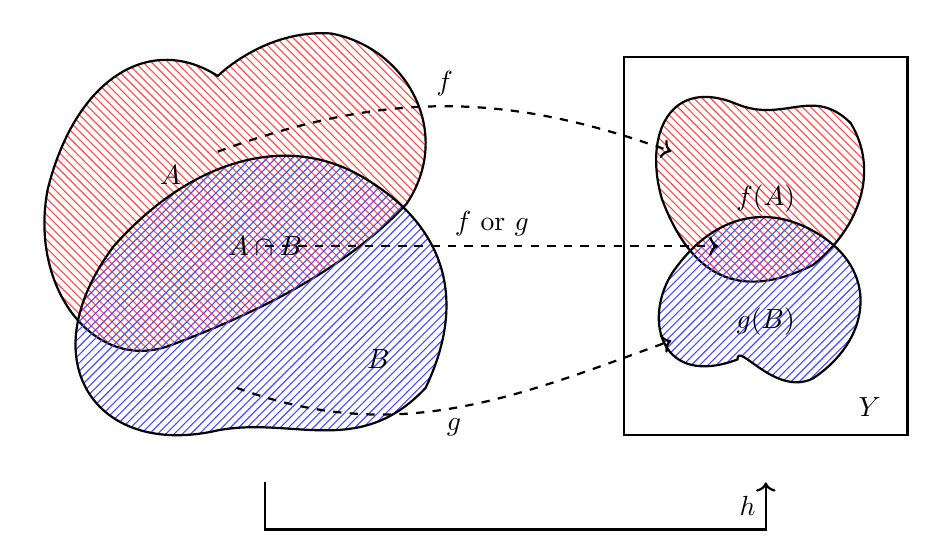
\begin{tikzpicture}[
        scale=1.2,
        set/.style={draw, thick},
        mapping/.style={->, thick},
        dashed mapping/.style={->, thick, dashed}
      ]
        % Set A with red north west lines pattern (smooth, asymmetric blob shape, vertically elongated)
        \begin{scope}
            \clip (-0.5,1.8) .. controls (-1.2,2.25) and (-2,1.8) .. 
                  (-2.3,0.6) .. controls (-2.5,-0.45) and (-1.8,-1.35) .. 
                  (-1,-1.05) .. controls (-0.2,-0.75) and (0.8,-0.3) .. 
                  (1.5,0.45) .. controls (2,1.2) and (1.5,2.1) .. 
                  (0.7,2.25) .. controls (0,2.3) and (-0.5,1.8) .. 
                  (-0.5,1.8) -- cycle;
            \fill[pattern=north west lines, pattern color=red!70] (-3,-3) rectangle (3,3);
        \end{scope}
        \draw[set] (-0.5,1.8) .. controls (-1.2,2.25) and (-2,1.8) .. 
                  (-2.3,0.6) .. controls (-2.5,-0.45) and (-1.8,-1.35) .. 
                  (-1,-1.05) .. controls (-0.2,-0.75) and (0.8,-0.3) .. 
                  (1.5,0.45) .. controls (2,1.2) and (1.5,2.1) .. 
                  (0.7,2.25) .. controls (0,2.3) and (-0.5,1.8) .. 
                  (-0.5,1.8) -- cycle;
        \node at (-1,0.75) {$A$};
        
        % Set B with blue north east lines pattern (asymmetric blob shape, vertically elongated)
        \begin{scope}
            \clip (-0.5,-1.95) .. controls (-1.8,-2.25) and (-2.5,-1.2) .. 
                  (-1.6,0) .. controls (-0.8,0.9) and (0.2,1.2) .. 
                  (1,0.75) .. controls (1.8,0.3) and (2.2,-0.45) .. 
                  (1.7,-1.5) .. controls (1,-2.25) and (0.3,-1.8) .. 
                  (-0.5,-1.95) -- cycle;
            \fill[pattern=north east lines, pattern color=blue!70] (-3,-3) rectangle (3,3);
        \end{scope}
        \draw[set] (-0.5,-1.95) .. controls (-1.8,-2.25) and (-2.5,-1.2) .. 
                  (-1.6,0) .. controls (-0.8,0.9) and (0.2,1.2) .. 
                  (1,0.75) .. controls (1.8,0.3) and (2.2,-0.45) .. 
                  (1.7,-1.5) .. controls (1,-2.25) and (0.3,-1.8) .. 
                  (-0.5,-1.95) -- cycle;
        \node at (1.2,-1.2) {$B$};
        
        % Add the intersection label
        \node at (0,0) {$A \cap B$};
        
        % Draw |___| shaped arrow at the bottom
        \draw[mapping] (0,-2.5) -- (0,-3) -- (5.3,-3) -- (5.3,-2.5) node[midway, left] {$h$};
        
        % Rectangle around right side (set Y)
        \draw[set] (3.8,-2) rectangle (6.8,2);
        \node at (6.4,-1.7) {$Y$};
        
        % Set f(A) on right with red north west lines pattern
        \begin{scope}
            \clip (5,1.5) .. controls (4.3,1.8) and (4,1.2) .. 
                  (4.2,0.5) .. controls (4.5,-0.3) and (5,-0.6) .. 
                  (5.8,-0.2) .. controls (6.3,0.2) and (6.5,0.8) .. 
                  (6.2,1.3) .. controls (5.8,1.7) and (5.5,1.3) .. 
                  (5,1.5) -- cycle;
            \fill[pattern=north west lines, pattern color=red!70] (3.5,-1) rectangle (7,2);
        \end{scope}
        \draw[set] (5,1.5) .. controls (4.3,1.8) and (4,1.2) .. 
                  (4.2,0.5) .. controls (4.5,-0.3) and (5,-0.6) .. 
                  (5.8,-0.2) .. controls (6.3,0.2) and (6.5,0.8) .. 
                  (6.2,1.3) .. controls (5.8,1.7) and (5.5,1.3) .. 
                  (5,1.5) -- cycle;
        \node at (5.3,0.5) {$f(A)$};
        
        % Set g(B) on right with blue north east lines pattern
        \begin{scope}
            \clip (5,-1.2) .. controls (4.2,-1.5) and (4,-0.8) .. 
                  (4.3,-0.3) .. controls (4.7,0.3) and (5.3,0.5) .. 
                  (5.9,0.1) .. controls (6.5,-0.3) and (6.4,-1) .. 
                  (5.8,-1.4) .. controls (5.4,-1.6) and (5,-1) .. 
                  (5,-1.2) -- cycle;
            \fill[pattern=north east lines, pattern color=blue!70] (3.5,-2) rectangle (7,1);
        \end{scope}
        \draw[set] (5,-1.2) .. controls (4.2,-1.5) and (4,-0.8) .. 
                  (4.3,-0.3) .. controls (4.7,0.3) and (5.3,0.5) .. 
                  (5.9,0.1) .. controls (6.5,-0.3) and (6.4,-1) .. 
                  (5.8,-1.4) .. controls (5.4,-1.6) and (5,-1) .. 
                  (5,-1.2) -- cycle;
        \node at (5.3,-0.8) {$g(B)$};
        
        % Dotted arrows for direct mappings
        \draw[dashed mapping] (-0.5,1) to[out=20, in=160] node[midway, above] {$f$} (4.3,1);
        \draw[dashed mapping] (-0.3,-1.5) to[out=-20, in=200] node[midway, below] {$g$} (4.3,-1);
        \draw[dashed mapping] (0,0) to[out=0, in=180] node[midway, above] {$f$ or $g$} (4.8,0);
      \end{tikzpicture}
      \caption{Visual of the pasting lemma.} 
      \label{fig:gluing_lemma}
    \end{figure}
  \end{lemma}

  Consider any set $U \subset Y$. Note that if $U$ is an open set in $X$ that happens to be contained in $Y$, then we can set $U = U \cap Y$, so $U$ is open in $Y$. However, we have seen that being open in $Y$ does not necessarily imply that it is open in $X$. 

  \begin{example}[Non-Open Sets may be Open in Subspace]
    Let $X = \mathbb{R}$ with the Euclidean topology and let $Y = [0, 1]$. 
    \begin{enumerate}
      \item $[0, 1]$ is open in $Y$ but not open in $X$. 
      \item Intervals of the form $(a, 1]$ and $[0, b)$ are open in $Y$ but not open (nor closed) in $X$. 
    \end{enumerate}
  \end{example} 

  \begin{example}[Singleton Sets in Subspace Topologies]
    Consider $X = \mathbb{R}$ with the lower limit topology with $Y = [0, 1]$. The following 
    \begin{enumerate}
      \item $[1/2, 1] = Y \cap [1/2, 2)$, and 
      \item $\{1\} = Y \cap [1, 2)$
    \end{enumerate}
    are open in the subspace topology. It turns out that $\{1\}$ is the only singleton set open in $Y$. 
  \end{example}

  Let's go through a few examples. 

  \begin{example}[Closed Unit Interval in $\mathbb{R}$]
    The basis for the subspace topology of $[0, 1] \subset \mathbb{R}$ with the Euclidean topology consists of the intervals 
    \begin{enumerate}
      \item $(a, b)$ where $0 \leq a < b \leq 1$. 
      \item $[0, b)$ where $0 < b \leq 1$. 
      \item $(a, 1]$ where $0 \leq a < 1$. 
    \end{enumerate}
  \end{example} 

  \begin{example}[Unit Sphere in $\mathbb{R}^n$] 
    Let $S^n \subset \mathbb{R}^{n+1}$ be the unit \textbf{n-sphere} defined $S^n \coloneqq \{x \in \mathbb{R}^{n+1} \mid ||x||^2 = 1 \}$. When thinking about $S^n$ as a space itself, we use the subspace topology coming from the standard topology of $\mathbb{R}^n$. 
  \end{example}

  \begin{example}[$S^1 \subset \mathbb{R}^2$]
    Let's focus on $n = 1$. For $a < b$, let 
    \begin{equation}
      A_{a, b} = \{ (\cos{t}, \sin{t}) \mid a < t < b \}
    \end{equation} 
    Then, we can see that
    \begin{enumerate}
      \item if $b - a > 2 \pi$, then $A_{a, b} = S^1$. 
      \item If $b - a \leq 2 \pi$, then $A_{a, b}$ is an ``open arc'' from $(\cos{a}, \sin{a})$ to $(\cos{b}, \sin{b})$.  
    \end{enumerate} 

    Given that we have an equivalence class defined 
    \begin{equation}
      A_{a, b} \sim A_{a + 2 \pi k, b + 2 \pi k} \text{ for all } k \in \mathbb{Z}
    \end{equation} 
    We claim that $\{A_{a, b}\}$ is a basis for the subspace topology of $S^1$. We can see that the open arc covering the top right quadrant in $\mathbb{R}^2$ is 
    \begin{equation}
      S^1 \cap (0, 1)^2 = S^1 \cap B_\infty \big( (\frac{1}{2}, \frac{1}{2}), \frac{1}{2} \big)
    \end{equation}
  \end{example}

  Now let's focus more on metric spaces. Note that if we want to construct topologies of subspaces of metric spaces, there are two ways to do it. It would be quite bad if these resulted in different topologies, but fortunately we have the following theorem. 

  \begin{theorem}[Topologies on Subspaces of Metric Spaces Coincide]
    Let $(X, d_X)$ be a metric space, with $Y \subset X$. There are 2 ways we can define a topology on $Y$. 
    \begin{enumerate}
      \item Take the metric topology $\T_X$ on $X$, and then take the subspace topology on $Y$. 
      \item Induce a metric $d_Y = d_{X | Y}$ on $Y$ which is a restriction of $d_X$ to $Y$, and then take the metric topology of it. 
    \end{enumerate}
    We claim that these two constructions give the same topology, as shown in the commutative diagram. 

    \begin{figure}[H]
      \centering 
      \begin{tikzcd}
        d_X \arrow[r] \arrow[d] & d_Y \arrow[d] \\
        \T_X \arrow[r] & \T_Y 
      \end{tikzcd}
      \caption{} 
      \label{fig:same_construction}
    \end{figure}
  \end{theorem}
  \begin{proof}
    The basis for the subspace topology on $Y$ is 
    \begin{equation}
      \B_1 = \{B_{d_X} (x, r) \cap Y \mid x \in X, r > 0 \}
    \end{equation} 
    and the basis for the (induced) metric topology on $Y$ is 
    \begin{equation}
      \B_2 = \{B_{d_Y} (y, r) \cap Y \mid y \in Y, r > 0 \} = \{B_{d_X} (y, r) \cap Y \mid y \in Y, r > 0 \}
    \end{equation} 
    It is immediate that $\B_2 \subset \B_1$ since it goes over all $x \in X$ rather than $y \in Y$. To see why $\B_1 \subset \B_2$, TBD. 
  \end{proof}

  \begin{theorem}[Closures in Subspace Topologies]
    Let $A \subset Y \subset X$. Let $\bar{A}$ denote the closure of $A$ in $X$. Then, the closure of $A$ in $Y$ equals $\bar{A} \cap Y$. 
  \end{theorem}

\subsection{Box Topology} 

  There are multiple ways to define the box and product topologies, but their construction with basis elements is most simple. 

  \begin{definition}[Box Topology]
    Given a family of topological spaces $\{(X_\alpha, \T_\alpha)\}_{\alpha \in A}$, the \textbf{box topology} on the space $\prod_{\alpha \in A} X_\alpha$ is the topology generated by the basis 
    \begin{equation}
      \mathscr{B} = \bigg\{ \prod_{\alpha \in A} U_\alpha \mid U_\alpha \in \T_\alpha \bigg\}
    \end{equation}

    \begin{figure}[H]
      \centering 
      \begin{tikzpicture}
        \draw[<->] (-1,0)--(6,0);
        \draw[<->] (0,-1)--(0,4);
        \draw[dashed] (1,1)--(1,3)--(4,3)--(4,1)--(1,1);
        \node[below] at (6,0) {$\mathbb{R}$};
        \node[left] at (0,4) {$\mathbb{R}$};
        \node[below] at (1,-0.3) {$a$};
        \node[below] at (4,-0.3) {$b$};
        \node[left] at (-0.3,1) {$c$};
        \node[left] at (-0.3,3) {$d$};
        \node[rotate=90] at (0,1) {$($};
        \node[rotate=-90] at (0,3) {$($};
        \node at (1,0) {$($};
        \node at (4,0) {$)$};
      \end{tikzpicture}
      \caption{We can visualize the elements of the box topology with the product space $\mathbb{R}^2 = \mathbb{R} \times \mathbb{R}$, where each $\mathbb{R}$ has an open ball topology. From the visual below, we can see why this is called the "box" topology. }
      \label{fig:box_topology}
    \end{figure}
  \end{definition}
  \begin{proof}
    It is easy to prove that the box topology indeed satisfies the 3 properties of topologies in general. 
  \end{proof}

\subsection{Product Topology}

  While the box topology may seem quite "intuitive" for the first learner, the box topology however, has serious limitations when extending to infinite Cartesian products of spaces. The main difference between the construction of open sets in the box topology vs the product topology is that the box topology merely describes open sets as direct products of open sets from each coordinate space while the construction of the product topology is completely dependent on the construction of the projection mappings 
  \begin{equation}
    \pi_\beta: \prod_{\alpha \in I} X_\alpha \rightarrow X_\beta
  \end{equation}
  to be continuous (and nothing more) so that (by definition) the preimages of open sets in $X_\beta$ under $\pi_\beta$ are open sets in $\prod X_\alpha$. Therefore, the construction of the continuous $\pi_\beta$'s canonically constructs a basis of open sets in $\prod X_\alpha$. 

  \begin{definition}[Product Topology] 
    Given a family of topological spaces $\{(X_\alpha, \T_\alpha)\}_{\alpha \in A}$, the \textbf{product topology} on the space $\prod_{\alpha \in A} X_\alpha$ is defined in the following equivalent ways. 
    \begin{enumerate}
      \item It is the initial topology on the product space wrt the family of projections $p_\alpha: \prod_{\alpha \in A} X_\alpha \rightarrow X_\alpha$. 

      \item It is the topology generated by the basis of elements 
      \begin{equation}
        \prod_\alpha U_\alpha 
      \end{equation}
      where $U_\alpha$ is a proper open subset for at most finitely many $\alpha$'s, and $U_\alpha = X_\alpha$ for all other $\alpha$. 
    \end{enumerate}

    \begin{figure}[H]
      \centering 
      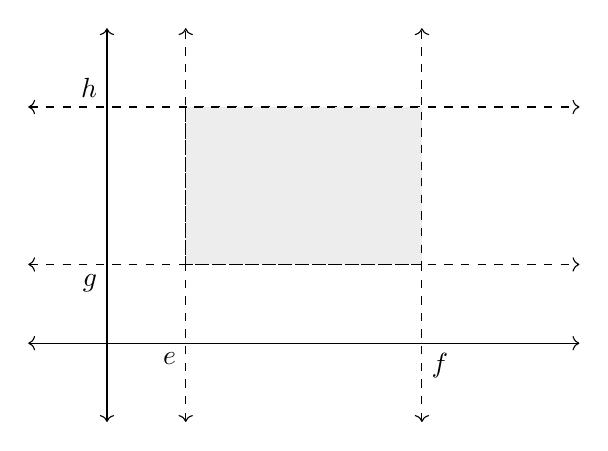
\begin{tikzpicture}
        \draw[<->] (-1,0)--(6,0);
        \draw[<->] (0,-1)--(0,4);
        \draw[<->, dashed] (-1,1)--(6,1);
        \draw[<->, dashed] (-1,3)--(6,3);
        \draw[<->, dashed] (1,-1)--(1,4);
        \draw[<->, dashed] (4,-1)--(4,4);
        \node [below left] at (1,0) {$e$};
        \node [below right] at (4,0) {$f$};
        \node [above left] at (0,3) {$h$};
        \node [below left] at (0,1) {$g$};
        \draw[dashed, fill=lightgray] (1,1) rectangle (4,3);
      \end{tikzpicture}
      \caption{Visually, we can interpret each $\mathscr{S} (U_\beta)$ as a "strip" in the total product space. For example in $\mathbb{R}^2$, there are two "strips" $(e, f) \times \mathbb{R}$ and $\mathbb{R} \times (g, h)$ that intersect. Note that each strip is the preimage of the projection mapping. }
      \label{fig:product_topology}
    \end{figure}
  \end{definition}

  We can deduce some conclusions comparing these topologies. First, the product and box topologies are precisely the same if we work in finite Cartesian products of spaces, since any element of the box topology (left hand side) can be expressed as a finite intersection of some open sets (in the right hand side). That is, if $\text{card}\,I < \infty$, then 
  \begin{equation}
    \prod_{\alpha \in I} U_i = \bigcap_{\alpha \in I} \big\{ \prod_{\gamma \in I} W_\gamma \mid W_\gamma = U_\gamma \text{ if } \gamma = \alpha, \, W_\gamma = X_\gamma \text{ if } \gamma \neq \alpha\big\}
  \end{equation}
  Secondly, we can see that the box topology is finer than the product topology (strictly finer if working in infinite product spaces). 

  \begin{example}
    The set $(0,1)^\mathbb{N} \subset \mathbb{R}^\mathbb{N}$ is clearly open in the box topology, but it is considered "too tight" to be in the product topology. However, 
    \begin{equation}
      (0,1) \times \mathbb{R} \times \mathbb{R} \times \ldots
    \end{equation}
    is open in the product topology since only one (a finite amount) of the factors is not the whole space. 
  \end{example}

  The following theorem reveals why the product topology is superior than the box topology in product spaces. 

  \begin{theorem}[Continuity of Functions Mapped to Product Topology]
    Given the function 
    \begin{equation}
      f: A \rightarrow \prod_{\alpha \in I} X_\alpha, \; f(a) \equiv \big( f_\alpha (a) \big)_{\alpha \in I}
    \end{equation}
    with its component functions $f_\alpha: A \rightarrow X_\alpha$. Let $\prod X_\alpha$ have the product topology. Then the function $f$ is continuous if and only if each function $f_\alpha$ is continuous. 
  \end{theorem}
  \begin{proof}
    We prove both directions. Let $\pi_\beta$ be the projection of this product onto the $\beta$th component space. By construction $\pi_\beta$ is continuous $\implies \pi_\beta^{-1} (U_\beta)$ is a basis element of the product topology of $\prod X_\alpha$. 
    \begin{enumerate}
      \item $(\rightarrow)$ $f$ is continuous, so $f_\beta \equiv \pi_\beta \circ f$, as the composition of continuous functions, is also continuous. 
      \item $(\leftarrow)$ Assume that each $f_\beta$ is continuous. Let there be an open set $U_\beta \subset X_\beta$. Then, the canonical open set $\pi_\beta^{-1}$ in the product space $\prod X_\alpha$ is also open. Now, the preimage of $\pi_\beta^{-1} (U_\beta)$ under $f$ is 
      \begin{align*}
        f^{-1} \big( \pi_\beta^{-1} (U_\beta)\big) & = (f^{-1} \circ \pi_\beta^{-1})(U_\beta) \\
        & = (\pi_\beta \circ f)^{-1} (U_\beta) \\
        & = f_\beta^{-1} (U_\beta)
      \end{align*}
      Since $f_\beta$ is already assumed to be continuous, $f_\beta^{-1} (U_\beta)$ is open in $A$. 
    \end{enumerate}
  \end{proof} 

  This theorem also works for the box topology only if we are working with finite product spaces. But in general, this theorem fails for the box topology. Consider the following example. 

  \begin{example}
    Let $\mathbb{R}^\omega$ be the countably infinite product of $\mathbb{R}$'s. Let us define the function 
    \begin{equation}
      f: \mathbb{R} \rightarrow \mathbb{R}^\omega
    \end{equation}
    with coordinate function defined $f_n (t) \equiv t$ for all $n \in \mathbb{N}$. Clearly, each $f_n$ is continuous. Given the box topology, we consider one basis element of $\mathbb{R}^\omega$
    \begin{equation}
      B = \prod_{i=1}^\infty (-\frac{1}{i}, \frac{1}{i})
    \end{equation}
    Assume that $f$ is continuous, that is $f^{-1}(B)$ is open in $\mathbb{R}$. Then, it would contain some finite interval $(-\delta, \delta)$ about $0$, meaning that $f\big( (-\delta, \delta)\big) \subset B$. This implies that for each $n \in \mathbb{N}$, 
    \begin{equation}
      f_n \big( (-\delta, \delta) \big) = (-\delta, \delta) \subset \Big( -\frac{1}{n}, \frac{1}{n} \Big)
    \end{equation}
    which contradicts the fact that $B$ is open, since the interval $(-1/n, 1/n)$ converges onto a point $0$. 
  \end{example}

  However, there is no useful criterion for the continuity of a mapping $f: X \times Y \longrightarrow A$ even if we have the product topology on $X \times Y$. One might conjecture that this $f$ is continuous if it is continuous in each variable separately, but this is in fact not true. 

  \begin{theorem}[Topologies on Products of Metric Spaces Coincide]
    Given a metric space
  \end{theorem}

  \begin{corollary}
    The Euclidean topology on $\mathbb{R}^n$ is equivalent to the product topology of the Euclidean topologies on $\mathbb{R}$. 
  \end{corollary}

  \begin{lemma}
    The addition, subtraction, and multiplication operations are continuous functions from $\mathbb{R} \times \mathbb{R} \longrightarrow \mathbb{R}$, and the quotient operation is a continuous function from $\mathbb{R} \times (\mathbb{R} \setminus \{0\}) \longrightarrow \mathbb{R}$. 
  \end{lemma}
  \begin{proof}
    Standard $\epsilon-\delta$ proof. 
  \end{proof}

  Now that we have defined what it means for binary operations to be continuous, we can talk about \textit{topological algebra}, which is the study of algebraic structures such that their algebraic operations and inverses are continuous. One important such concept is a \textit{topological group}, which will be mentioned later. 

\subsection{Quotient Topologies} 

  We have established natural topologies on sets that are constructed from other sets, namely by subsets and Cartesian products. Another way to construct a set is by taking an \hyperref[set-partition]{equivalence relation}, which partitions the set into its equivalence classes. The method in which we construct such a topology on this quotient space, called the \textit{quotient topology}, is slightly less straightforward.  

  \subsubsection{Quotient Maps}

    \begin{definition}[Quotient Map]
      A function $p: X \rightarrow Y$ is said to be a \textbf{quotient map} if it is surjective and 
      \begin{equation}
        U \text{ is open in } Y \iff p^{-1}(U) \text{ is open in } X
      \end{equation} 
      Note that we could have also replaced open with closed sets and the definitions are equivalent. 
    \end{definition}

    \begin{definition}[Saturation]
      A subset $S \subset X$ is \textbf{saturated} with respect to the surjective map $p: X \rightarrow Y$ if for every $p^{-1} (A)$ (where $A \subset Y$) that intersects $S$, $p^{-1}(A)$ is completely contained within $S$. That is, 
      \begin{equation}
        p^{-1} \big( p(S) \big) = S
      \end{equation}

      \begin{figure}[H]
        \centering 
        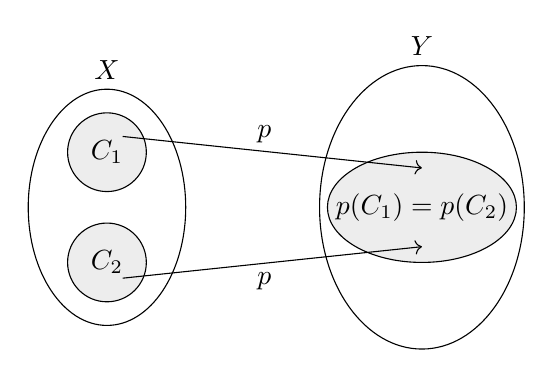
\begin{tikzpicture}
          \draw (0,0) ellipse (1 and 1.5);
          \draw[fill=lightgray] (0, 0.7) circle (0.5);
          \draw[fill=lightgray] (0, -0.7) circle (0.5);
          \node[above] at (0,1.5) {$X$};
          \draw (4,0) ellipse (1.3 and 1.8);
          \node[above] at (4,1.8) {$Y$};
          \draw[fill=lightgray] (4,0) ellipse (1.2 and 0.7);
          \node at (0, 0.7) {$C_1$};
          \node at (0,-0.7) {$C_2$};
          \node at (4,0) {$p(C_1) = p(C_2)$};
          \draw[->] (0.2,0.9)--(4,0.5);
          \draw[->] (0.2,-0.9)--(4,-0.5);
          \node[above] at (2, 0.7) {$p$};
          \node[below] at (2, -0.7) {$p$};
        \end{tikzpicture}
        \caption{We can see that $C_1$ and $C_2$ alone are not saturated, but $C_1 \cup C_2$ is saturated. Visually, for a given set $C \subset X$ to be saturated, there cannot be any points $q \not\in C$ such that $q \in p(C)$. }
        \label{fig:saturation}
      \end{figure}
    \end{definition}

    We now introduce an alternative, equivalent definition of quotient maps. 

    \begin{theorem}[Quotient Maps w.r.t. Mapping Saturated Sets]
      $p: X \rightarrow Y$ is a quotient map if and only if $p$ is continuous and $p$ maps saturated open sets of $X$ to open sets of $Y$ (or saturated closed sets of $X$ to closed sets of $Y$). 
    \end{theorem} 

    The first property is that quotient maps behave nicely under compositions. 

    \begin{theorem}[Composition of Quotient Maps]
      The composition of two quotient maps is a quotient map. 
    \end{theorem}
    \begin{proof}
      We immediately know that the composition of surjective maps are surjective and that of continuous maps are continuous. 
    \end{proof}

    However, they do not behave nicely under subspace or products. If $p: X \rightarrow Y$ is a quotient map and $A$ is a subspace of $X$, then the map $p^\prime: A \rightarrow p(A)$ obtained by restricting both the domain and codomain of $P$ need not be a quotient map. The product of two quotient maps is not necessarily a quotient map. That is, given $p: A \rightarrow B$ and $q: C \rightarrow D$ are quotient maps, the map 
    \begin{equation}
      p \times q: A \times C \rightarrow B \times D, \; (p \times q) (a \times c) \equiv p(a) \times q(c)
    \end{equation}
    is not necessarily a quotient map. 

    \begin{example}[Restriction of Quotient Maps are Not Quotient Maps]
      
    \end{example}

    \begin{example}[Products of Quotient Maps are Not Quotient Maps]
      
    \end{example}

    Additionally, quotient maps are clearly not homeomorphisms, so topological properties are not preserved. 

    \begin{example}[]
      
    \end{example}

    However, there is just one extra condition on a quotient map that will make it a homeomorphism.  

    \begin{lemma}[Bijective Quotient Maps]
      A quotient map that is injective (and hence bijective) is a homeomorphism. 
    \end{lemma} 

  \subsubsection{Open and Closed Maps}

    Open and closed functions map open/closed sets to open/closed sets, unlike continuous functions which take the preimage. However, they do are not natural and most maps are not open nor closed, so this is a pretty special condition. 

    \begin{definition}[Open, Closed Maps]
      A map $f: X \rightarrow Y$ is said to be 
      \begin{enumerate}
        \item \textbf{open} if it maps open sets of $X$ to open sets of $Y$. 
        \item \textbf{closed} if it maps open sets of $X$ to closed sets of $Y$. 
      \end{enumerate}
      Note that open and closed maps are completely independent. A map may be open, closed, neither, or both. 
    \end{definition}

    \begin{example}[Open but Not Closed]
      The projection $\pi_1: X \times Y \rightarrow X$ is an open map but but closed. Consider $\pi_1: \mathbb{R}^2 \rightarrow \mathbb{R}$ with $S = \{(x, y) \in \mathbb{R}^2 \mid xy = 1 \}$. Then $\pi_1 (S) = \mathbb{R} \setminus \{0\}$, which is not closed.\footnote{In open maps, the typical behavior is that points are ``copied,'' i.e. for projections, the preimage of $\pi_1^{-1} (x) = x \times Y$, where all $y \in Y$ are copied.}
    \end{example}

    \begin{example}[Closed but Not Open]
      $f: \mathbb{R} \rightarrow \mathbb{R}$ with $f(x) = x^2$ is closed but not open since $f(\mathbb{R}) = [0, +\infty)$ which is not open. 
    \end{example}

    Note that an open map or a closed map (with continuous and surjective) are trivially quotient maps. Since given a $U \subset Y$ with $f^{-1} (U)$ open, then by definition $U = f(f^{-1} (U))$ is open by definition. 

    \begin{theorem}[Open/Closed Maps are Stronger than Quotient Maps]
      If $p: X \rightarrow Y$ is a surjective, continuous map that is either open or closed (that is, maps open sets to open sets or closed sets to closed sets), then $p$ is a quotient map.\footnote{Note however, that the converse is not true; there exists quotient maps that are neither open nor closed. }
    \end{theorem} 

    \begin{example}[Quotient Maps that are Neither Open Nor Closed]
      
    \end{example}

  \subsubsection{Quotient Topology}

    Now that we have defined the quotient map, we are ready to define the quotient topology. 

    \begin{definition}[Quotient Topology]
      Let $p: (X, \T_X) \rightarrow Y$ be a surjective map.\footnote{A natural surjective map that we can construct is by taking an equivalence relation $\sim$ on $X$, setting $Y = X/\sim$, and taking $p: x \mapsto [x]$. Every surjective map can be thought of as a map induced by an equivalence relation, since we can set $x \sim x^\prime$ iff $f(x) = f(x^\prime)$, so these are equivalent.} Then, the \textbf{quotient topology} induced by $p$ is defined in the following equivalent ways. 
      \begin{enumerate}
        \item It is the final topology on the quotient set $X/\sim$ wrt the projection map $p$. 
        \item It is the topology of all subsets $U$ of $Y$ s.t. $p^{-1}$ is open in $X$. 
        \begin{equation}
          U \text{ open in } X/\sim \iff p^{-1} (U) \text{ saturated and open in } X
        \end{equation}
        \item It is the unique topology $\T_Y$ relative to which $p$ is a quotient map.\footnote{We claim that this topology exists and is unique.}
      \end{enumerate}
      The quotient set $X/\sim$ with its quotient topology is called the \textbf{quotient space}. 
    \end{definition}
    \begin{proof}
      The topology $\T_Y$ on $Y$ is defined by letting it consist of all subsets $U$ of $Y$ such that $p^{-1}(U)$ is open in $X$. This is indeed a topology since
      \begin{enumerate}
        \item $p^{-1} (\emptyset) = \emptyset$ and $p^{-1}(Y) = X$
        \item $p^{-1} \Big( \bigcup_{\alpha \in J} U_\alpha \Big) = \bigcup_{\alpha \in J} p^{-1} (U_\alpha)$
        \item $p^{-1} \Big( \bigcap_{i=1}^n U_i \Big) = \bigcap_{i=1}^n p^{-1} (U_i)$
      \end{enumerate}
    \end{proof}

    The intuition is the following. The topology on $X$ is fixed, and we must somehow find some topology on $Y$ that makes $p$ a quotient map. If we make $\T_Y$ too coarse, satisfiying continuity of $p$ is easy but it may not necessarily mean that $p^{-1}(U)$ open in $X$ implies $U$ open in $Y$. However, if we make $\T_Y$ too fine, then continuity may not be satisifed. The theorem states that there is a middle point---in fact exactly one topology---in which cases both directions are satisfied. 

    \begin{example}
      Let $p: (\mathbb{R}, \T_\mathbb{R}) \rightarrow \mathbb{R} / 2 \pi \mathbb{R}$. Then, the final topology of $\mathbb{R} / 2 \pi \mathbb{R}$ would be simply defined 
      \begin{equation}
        \T_{\mathbb{R} / 2 \pi \mathbb{R}} \equiv \{U \subset \mathbb{R} / 2\pi \mathbb{R} \mid U = p(O), O \in \T_\mathbb{R}\}
      \end{equation}
      That is, the quotient topology is merely the set of all images of open sets in $\mathbb{R}$ under $f$. However, if $\mathbb{R} / 2 \pi \mathbb{R}$ has the discrete topology $2^X$, then a single equivalence class, say $[0]$, will get mapped to the collection of points $\{2 \pi k \mid k \in \mathbb{Z}\}$, which is clearly not open in $\mathbb{R}$. Note that the final topology (or the quotient topology) is endowed onto the codomain in order to make $f$ continuous (or a quotient mapping). 
    \end{example}

    \begin{example}
      Let $X \equiv [0,1] \cap [2,3] \subset \mathbb{R}$ and $Y y \equiv [0,2] \subset \mathbb{R}$. Then, we define $p: X \rightarrow Y$ as 
      \begin{equation}
        p(x) \equiv \begin{cases} x & x \in [0,1] \\ x-1 & x \in [2,3] \end{cases}
      \end{equation}
      $p$ is continuous (under subspace topology of $X \subset \mathbb{R}$), surjective, and closed, meaning that it is a quotient map. However, it is not open, since the image of the open set $[0,1]$ of $X$ is $[0,1]$, which is not open in $Y$. 
    \end{example}

    \begin{example}[Finite Sets]
      Let $p: \mathbb{R} \rightarrow \{a, b, c\}$ be defined as 
      \begin{equation}
        p(x) \equiv \begin{cases} a & x > 0 \\ b & x < 0 \\ c & x = 0 \end{cases}
      \end{equation}
      Then, the quotient topology of $\{a, b, c\}$ consists of 
      \begin{equation}
        \emptyset, \{a\}, \{b\}, \{a, b\}, \{a, b, c\}
      \end{equation}
    \end{example}

    Okay, so we've learned yet another way to construct topologies. However, things become interesting when we start to compare quotient spaces to other topological spaces that we already know of. The following series of theorems will help in our analysis. 

    \begin{theorem}[Induced Maps from Quotient Space]
      Let $p: X \rightarrow Y$ be a quotient map (e.g. $Y = X/\sim$ for some ER $\sim$). Let $f: X \rightarrow Z$ be a function such that if $p(x) = p(x^\prime)$, then $f(x) = f(x^\prime)$, i.e. $x \sim x^\prime \iff f(x) = f(x^\prime)$. Then, 
      \begin{enumerate}
        \item $f$ induces the map $\bar{f}$ satisfying $f = \bar{f} \circ p$. 

        \begin{figure}[H]
          \centering 
          \begin{tikzcd}
            X \arrow{d}{p} \arrow{r}{f} & Z\\
            X/\sim \arrow{ru}{\bar{f}} & 
          \end{tikzcd}
          \caption{The theorem states that the diagram commutes. } 
          \label{fig:quotient_continuity}
        \end{figure}

        \item $f$ continuous iff $\bar{f}$ continuous. 
        \item $f$ quotient map iff $\bar{f}$ quotient map. 
      \end{enumerate}
    \end{theorem}
    \begin{proof}
      Listed. 
      \begin{enumerate}
        \item 
        \item Suppose $f$ is continuous. Let $U \subset Z$ be open. Then we need to show that $\bar{f}^{-1} (U)$ is open. But we can see that $p^{-1} (\bar{f}^{-1}(U)) = f^{-1} (U)$ is open since $f$ is continuious. Therefore $\bar{f}^{-1} (U)$ is open since $p$ is a QM.If $\bar{f}$ is continuous, then $f = \bar{f} \circ p$ is continuous as the composition of continuous maps. 
        \item Suppose $f$ is a quotient map with $U \subset Z$ s.t. $\bar{f}^{-1} (U)$ is open. We need to show that $U$ is open. Then $p^{-1} (\bar{f}^{-1} (U))$ is open since $p$ is continuous $\implies f^{-1} (U)$ is open. But $f$ is a quotient map, so $U$ is open. 
      \end{enumerate}
    \end{proof}

    \begin{corollary}
      If $f$ is a quotient map, then $\bar{f}$ is a homeomorphism. 
    \end{corollary}
    \begin{proof}
      Show that $\bar{f}$ is injective, and so its bijective. Since it's a quotient map, it's a homeomorphism. 
    \end{proof}

    Therefore we can just make up any equivalence relation (surjective map) on $X$ which gives us a quotient space $X/\sim$. To figure out whether this quotient space is homeomorphic to a topological space that we already know, we first (cleverly) choose a candidate space $Z$ and try to write a quotient map $f: X \rightarrow Z$ that ``agrees'' with the equivalence relation, i.e. $x \sim x^\prime \iff f(x) = f(x^\prime)$. We don't need to worry too much about surjectivity, since if we have continuity and the ``reverse continuity'' conditions satisfied then we can just restrict $Z$ to the image of $f$ to make it surjective anyways. Once we have found such a quotient map $f$, using the theorem above we can conclude that $X/\sim$ is homeomorphic to $Z$, and we are done! We show various examples below. 

    \begin{example}[1-Sphere]
      Let $X = [0, 1]$ with $\sim$ defined only with $0 \sim 1$. Then we can think of it as being similar to the unit circle $S^1$. 

      \begin{figure}[H]
        \centering
        \begin{subfigure}[b]{0.48\textwidth}
          \centering
          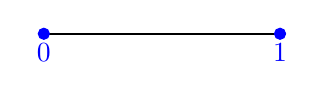
\begin{tikzpicture}
            % Draw the line segment from 0 to 1
            \draw[thick] (0,0) -- (3,0);
            
            % Draw blue endpoints
            \filldraw[blue] (0,0) circle (2pt) node[below] {0};
            \filldraw[blue] (3,0) circle (2pt) node[below] {1};
          \end{tikzpicture}
          \caption{Unit interval $[0, 1]$}
          \label{fig:unit-interval}
        \end{subfigure}
        \hfill 
        \begin{subfigure}[b]{0.48\textwidth}
          \centering
          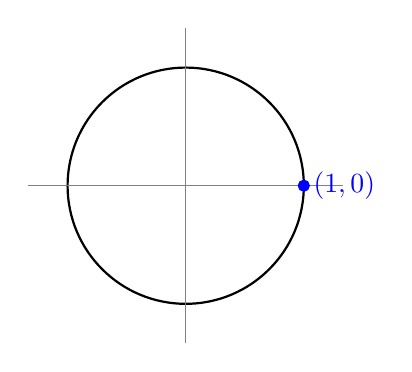
\begin{tikzpicture}
            % Draw the unit circle
            \draw[thick] (0,0) circle (1.5);
            
            % Draw axes for reference
            \draw[gray, thin] (-2,0) -- (2,0);
            \draw[gray, thin] (0,-2) -- (0,2);
            
            % Mark the point (1,0) in blue
            \filldraw[blue] (1.5,0) circle (2pt) node[right] {$(1,0)$};
          \end{tikzpicture}
          \caption{Unit circle $S^1$ in $\mathbb{R}^2$}
          \label{fig:unit-circle}
        \end{subfigure}
        \caption{Visual of the homeomorphism between $[0, 1]$ and $S^1$.}
        \label{fig:comparison}
      \end{figure}

      So can I come up with a function $f: [0, 1] \rightarrow S^1$ s.t. $f(0) = f(1)$? Yes, we can define 
      \begin{equation}
        \bar{f}(x) = (\cos{2 \pi x}, \sin{2\pi x})
      \end{equation}
      Note that we could just chosen $\mathbb{R}^2$ and restricted the image to $S^1$ at the end as well. Therefore, by the theorem above, $X/\sim \cong S^1$, defined by the homeomorphism $\bar{f}(x) = (\cos{2 \pi x}, \sin{2\pi x})$.  
    \end{example}

    \begin{example}[Alternative Construction of 1-Sphere]
      We will show that
      \begin{equation}
        \frac{\mathbb{R}}{\mathbb{Z}} \cong S^1
      \end{equation}
      Let us construct the set $(\mathbb{R}, \T_{\mathbb{R}})$ with paramater $t$. We define maps
      \begin{align*}
        p: \mathbb{R} \rightarrow \mathbb{R} / \mathbb{Z}, \;\; p(t) \equiv t \; (\text{mod } 1) \\
        q: \mathbb[R] \rightarrow S^1 \subset \mathbb{C}, \;\; g(t) \equiv e^{2 \pi i t} 
      \end{align*}
      We claim that $p$ and $q$ are both quotient mappings. Clearly, $p$ is a quotient mapping. As for $q$, it it easy to see that it is surjective (but not injective) and continuous ($\T_{S^1}$ has the basis of open intervals on $S^1$). It is also easy to notice that given an open interval $U \subset S^1$, $q^{-1}(U)$ will be the union of open intervals equally spaced in $\mathbb{R}$. Additionally, given any open interval in $\mathbb{R}$, it maps to an open interval in $S^1$ (note that $S^1$ itself is also open). These three conditions imply that $q$ is a quotient map. We now define maps 
      \begin{align}
        q \circ p^{-1}: & \mathbb{R} / \mathbb{Z} \rightarrow S^1 \\
        p \circ q^{-1}: & S^1 \rightarrow \mathbb{R} / \mathbb{Z}
      \end{align}
      and claim that these maps are homeomorphisms. We can clearly see that the mapping from an open set in $\mathbb{R} / \mathbb{Z}$ to the union of spaced open intervals in $\mathbb{R}$ is an injection, and the mapping from this union of open intervals to the union of open intervals in $S^1$ is a surjection. The composition of these two mappings clearly defines a bijection. Therefore, $q \circ p^{-1}$ is proven to be a bicontinuous bijective mapping between open sets $U \subset \mathbb{R} / \mathbb{Z}$ and $V \subset S^1 \implies$ $q \circ p^{-1}$ is a homeomorphism. 

      This result clearly makes sense since 
      \begin{equation}
        \frac{\mathbb{R}}{\mathbb{Z}} \cong \frac{[0,1]}{\sim}
      \end{equation}
      where the relation $\sim$ maps every point $x \in (0,1)$ to its own equivalence class and the points $0, 1$ to one equivalence class $\{0\}$. Therefore, it is informally said that the quotient space of the real line is a circle. 

      One may attempt to construct a simpler set by replacing $S^1$ with the half-open interval $[0,1)$. However, while $[0,1)$ is bijective to $\mathbb{R} / \mathbb{Z}$,
      \begin{equation}
        \frac{\mathbb{R}}{\mathbb{Z}} \not\cong [0,1)
      \end{equation}
      That is, the two sets are not homeomorphic because the topologies of $[0,1)$ and $\mathbb{R} / \mathbb{Z}$ are not compatible. For instance, when we attempt to map the open set 
      \begin{equation}
        \bigg\{ [x] \in \mathbb{R} / \mathbb{Z} \mid 0 \leq x \leq \frac{1}{4} \vee x > \frac{1}{2} \bigg\} \in \T_{\mathbb{R} / \mathbb{Z}}
      \end{equation}
      to $\T_{[0,1)}$, it does not return an open set. 

      Furthermore, this means that
      \begin{equation}
        S^1 \times S^1 \cong \frac{[0,1]^2}{\sim^\prime} \cong \bigg( \frac{\mathbb{R}}{\mathbb{Z}} \bigg)^2
      \end{equation}
      where $\sim^\prime$ is the quotient mapping defined in the previous construction of the torus. 
    \end{example}

    \begin{example}[Annulus]
      We can construct an annulus with the homeomorphism 
      \begin{equation}
        (x, y) \mapsto \big( (1 + y) \cos{2 \pi x}, (1 + y) \sin{2 \pi x} \big) \in \mathbb{R}^2
      \end{equation}

      \begin{figure}[H]
        \centering
        \begin{subfigure}[b]{0.48\textwidth}
          \centering
          \begin{tikzpicture}
            % Draw square
            \draw (0,0) rectangle (2,2);
            
            % Label top and bottom with >
            \node at (1,2) {$>$};
            \node at (1,-0) {$>$};
          \end{tikzpicture}
          \caption{Unit square $[0,1] \times [0,1]$}
          \label{fig:unit-square}
        \end{subfigure}
        \hfill 
        \begin{subfigure}[b]{0.48\textwidth}
          \centering
          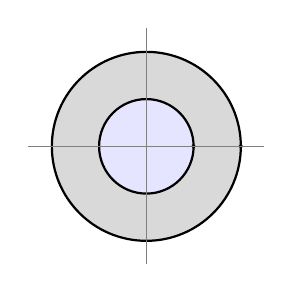
\begin{tikzpicture}[scale=0.6]
            % Fill the annular region with grey (using even-odd rule to keep the inner circle empty)
            \begin{scope}
              \clip (0,0) circle (2);
              \fill[gray!30] (0,0) circle (2);
              \fill[blue!10] (0,0) circle (1);
            \end{scope}
            
            % Draw the two circles
            \draw[thick] (0,0) circle (1);   % Unit circle
            \draw[thick] (0,0) circle (2);   % Circle of radius 2
            
            % Label only the points (1,0) and (2,0)
            \filldraw[font=\footnotesize] (1,0) circle (1pt) node[below] {};
            \filldraw[font=\footnotesize] (2,0) circle (1pt) node[below] {};

            \draw[gray, thin] (-2.5,0) -- (2.5,0);
            \draw[gray, thin] (0,-2.5) -- (0,2.5);
          \end{tikzpicture}
          \caption{Annular region between circles of radius 1 and 2}
          \label{fig:annular-region}
        \end{subfigure}
        \caption{Unit square and annular region}
        \label{fig:annular_comparison}
      \end{figure}
    \end{example}

    \begin{example}[Cylinder]
      Given the unique square $[0, 1]^2$, we can define the equivalence map as $(0, y) \sim (1, y)$ for $y \in [0, 1]$. We claim that this is homeomorphic to the cylinder 
      \begin{equation}
        C \equiv \{(x, y, z) \in \mathbb{R}^3 \mid x^2 + y^2 = 1, z \in [0,1]\} 
      \end{equation}
      with the homeomorphism 
      \begin{equation}
        (x, y) \mapsto \big( \cos{2\pi x}, \sin{2 \pi x}, y \big)
      \end{equation}

      \begin{figure}[H]
        \centering
        \begin{subfigure}[b]{0.48\textwidth}
          \centering
          \begin{tikzpicture}
            % Draw square
            \draw (0,0) rectangle (2,2);
            
            % Label top and bottom with >
            \node at (1,2) {$>$};
            \node at (1,-0) {$>$};
          \end{tikzpicture}
          \caption{Cylinder as an equivalence class on $[0, 1]^2$.}
          \label{fig:cylinder_equiv}
        \end{subfigure}
        \hfill 
        \begin{subfigure}[b]{0.48\textwidth}
          \centering
          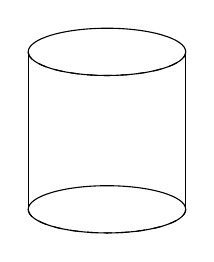
\begin{tikzpicture}
            % Draw cylinder
            \draw (0,0) ellipse (1 and 0.3);
            \draw (0,2) ellipse (1 and 0.3);
            \draw (-1,0) -- (-1,2);
            \draw (1,0) -- (1,2);
            
            % Draw dashed lines to show back of cylinder
            \draw[dashed] (-1,0) arc (180:360:1 and 0.3);
            \draw[dashed] (-1,2) arc (180:360:1 and 0.3);
          \end{tikzpicture}
          \caption{Cylinder as an embedding in $\mathbb{R}^2$. }
          \label{fig:cylinder_embed}
        \end{subfigure}
        \caption{Two geometric figures: a square with labeled sides and a cylinder}
        \label{fig:cylinder}
      \end{figure}
    \end{example}

    \begin{example}[Torus]
      Let $X \equiv [0,1] \times [0,1] \subset \mathbb{R}^2$. We define an equivalence relation $Y$ consisting of the equivalence classes
      \begin{align*}
          &\big\{\{(x, y)\} \mid 0<x, y<1\big\} \cup \big\{ \{(x, 0), (x,1)\} \mid 0<x<1 \big\} \cup \\
          &\big\{ \{(0,y), (1,y)\} \mid 0<y<1 \big\} \cup \big\{ \{(0,0), (0,1), (1,0), (1,1)\} \big\}
      \end{align*} 

      \begin{figure}[H]
        \centering 
        \begin{tikzpicture}
          \draw (0,0) rectangle (2,2);
          \draw (3,0) rectangle (5,2);
          \draw (6,0) rectangle (8,2);
          \draw (9,0) rectangle (11,2);
          \draw[dashed] (1, 1.5) circle [radius=0.4];
          \draw[fill] (1, 1.5) circle [radius=0.03];
          \draw[dashed] (3.9,0) arc (0:180: 0.4);
          \draw[dashed] (3.9,2) arc (0:-180:0.4);
          \draw[dashed] (6,1.1) arc (-90:90:0.4);
          \draw[dashed] (8,1.9) arc (90:270:0.4);
          \draw[fill] (3.5,0) circle [radius=0.03];
          \draw[fill] (3.5,2) circle [radius=0.03];
          \draw[fill] (6,1.5) circle [radius=0.03];
          \draw[fill] (8,1.5) circle [radius=0.03];
          \draw[fill] (9,0) circle [radius=0.03];
          \draw[fill] (11,0) circle [radius=0.03];
          \draw[fill] (9,2) circle [radius=0.03];
          \draw[fill] (11,2) circle [radius=0.03];
          \draw[dashed] (9.4,0) arc (0:90:0.4);
          \draw[dashed] (9.4,2) arc (0:-90:0.4);
          \draw[dashed] (11,0.4) arc (90:180:0.4);
          \draw[dashed] (10.6,2) arc (180:270:0.4);
        \end{tikzpicture}
        \caption{The quotient topology of this quotient space consists of open sets of form. } 
        \label{fig:torus_basis}
      \end{figure}
      This quotient space $X / Y$ is homeomorphic to the torus $S^1 \times S^1$, denoted
      \begin{equation}
        \frac{X}{Y} \cong S^1 \times S^1
      \end{equation}
      We can visualize the construction of the equivalence relation $Y$ as a "gluing" of the rectangle $X$ by its edges and corners. 

      \begin{figure}[H]
        \centering
        \begin{subfigure}[b]{0.48\textwidth}
          \centering
          \begin{tikzpicture}
            % Draw square
            \draw (0,0) rectangle (2,2);
            
            % Label top and bottom with >
            \node at (1,2) {$>$};
            \node at (1,0) {$>$};
            
            % Add >> labels to left and right sides, rotated to point upward
            \node[rotate=90] at (0,1) {$>>$};
            \node[rotate=90] at (2,1) {$>>$};
          \end{tikzpicture}
          \caption{Square with top and bottom sides labeled with $>$}
          \label{fig:square_torus}
        \end{subfigure}
        \hfill 
        \begin{subfigure}[b]{0.48\textwidth}
          \centering
          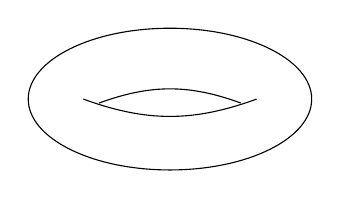
\begin{tikzpicture}
            % Draw torus similar to the reference image
            % Outer ellipse (complete)
            \draw (0,0) ellipse (1.8 and 0.9);
            
            % Inner curves (representing the hole)
            \draw (-0.9, -0.05) to[out=20,in=-200] (0.9, -0.05);
            \draw (-1.1, 0) to[out=-20,in=200] (1.1, 0);
          \end{tikzpicture}
          \caption{Torus}
          \label{fig:torus}
        \end{subfigure}
        \caption{Two geometric figures: a square with labeled sides and a torus}
        \label{fig:geometric-figures}
      \end{figure}
      
      We can check that this mapping is indeed a quotient map. First, it is clearly surjective. By realizing that individual points on the edge of $[0,1]^2$ are open sets themselves (by the subspace topology), we can prove that this map is indeed open and continuous. 
    \end{example}

    \begin{example}[Mobius Strip]
      We can construct the Mobius strip on $[0, 1]^2$ with the equivalence class $(0, y) \sim (1, 1 - y)$ for $y \in [0, 1]$. An explicit parameterization is quite tedious, but we can write the embedding $M \rightarrow \mathbb{R}^3$ with cylindrical coordinates. 
      \begin{figure}[H]
        \centering
        \begin{subfigure}[b]{0.48\textwidth}
          \centering
          \begin{tikzpicture}
            % Draw square
            \draw (0,0) rectangle (2,2);
            
            % Label top and bottom with >
            \node at (1,2) {$>$};
            \node at (1,-0) {$<$};
          \end{tikzpicture}
          \caption{Cylinder as an equivalence class on $[0, 1]^2$.}
          \label{fig:mobius_equiv}
        \end{subfigure}
        \hfill 
        \begin{subfigure}[b]{0.48\textwidth}
          \centering 
          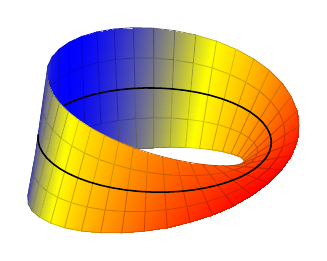
\begin{tikzpicture}[scale=0.7]
            \begin{axis}[
                hide axis,
                view={40}{40}
            ]
            \addplot3 [
                surf, shader=faceted interp,
                point meta=x,
                samples=40,
                samples y=5,
                z buffer=sort,
                domain=0:360,
                y domain=-0.5:0.5
            ] (
                {(1+0.5*y*cos(x/2)))*cos(x)},
                {(1+0.5*y*cos(x/2)))*sin(x)},
                {0.5*y*sin(x/2)});

            \addplot3 [
                samples=50,
                domain=-145:180, % The domain needs to be adjusted manually, depending on the camera angle, unfortunately
                samples y=0,
                thick
            ] (
                {cos(x)},
                {sin(x)},
                {0});
            \end{axis}
          \end{tikzpicture} 
          \caption{Mobius strip has 1 side and is a non-orientable surface.} 
          \label{fig:mobius_strip_r3}
        \end{subfigure}
        \caption{Two geometric figures: a square with labeled sides and a cylinder}
        \label{fig:mobius_strip}
      \end{figure}
    \end{example}

    \begin{example}[2-Sphere]
      Let $X$ be the closed unit ball 
      \begin{equation}
        X \equiv \{(x, y) \in \mathbb{R}^2 \mid x^2 + y^2 \leq 1\}
      \end{equation}
      and define the equialence classes $R$ as 
      \begin{equation}
        R \equiv \big\{ \{(x, y)\} \mid x^2 + y^2 <1 \big\} \cup \{S^1\}
      \end{equation}
      which will consist of open sets of one of the two forms
      \begin{center}
      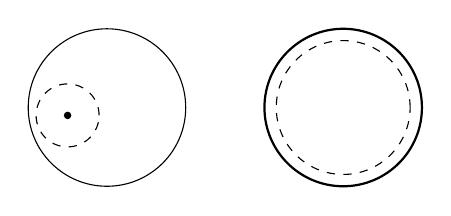
\begin{tikzpicture}
        \draw (1,1) circle [radius=1];
        \draw[thick] (4,1) circle [radius=1];
        \draw[dashed] (0.5,0.9) circle [radius=0.4];
        \draw[fill] (0.5,0.9) circle [radius=0.04];
        \draw[dashed] (4,1) circle [radius=0.85];
      \end{tikzpicture}
      \end{center}
      Then, this quotient space $X / R$ is homeomorphic to the 2-sphere
      \begin{equation}
        S^2 \equiv \{(x, y, z) \in \mathbb{R}^3 \mid x^2 + y^2 + z^2 = 1\}
      \end{equation}
      Visually, we can imagine the disk being glued together by its sides to continuously form the 2-sphere. 
    \end{example}

    \begin{example}[Weird Quotient Space]
      Given $(\mathbb{R}, \T_{\mathbb{R}})$, let us define the relation $\sim$ determined by the quotient mapping 
      \begin{equation}
        p(x) \equiv \begin{cases} \{x\} & x \not\in \mathbb{Z} \\ \mathbb{Z} & x \in \mathbb{Z} \end{cases}
      \end{equation}
      In words, this quotient map maps every integer to the equivalence class $[0]$ and maps every other point to its own class. 

      \begin{figure}[H]
        \centering 
        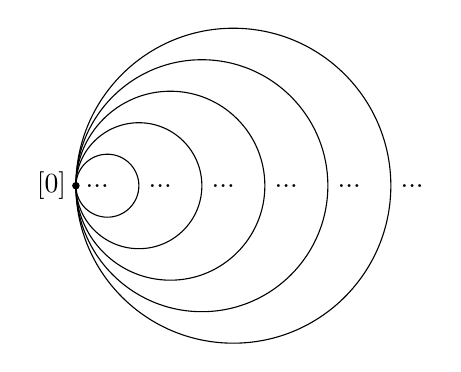
\begin{tikzpicture}[scale=0.4]
          \draw (5,0) circle (5);
          \node[left] at (0,0) {$[0]$};
          \draw[fill] (0,0) circle (0.1);
          \draw (4,0) circle (4);
          \draw (3,0) circle (3);
          \draw (2,0) circle (2);
          \draw (1,0) circle (1);
          \node[right] at (0,0) {...};
          \node[right] at (2,0) {...};
          \node[right] at (4,0) {...};
          \node[right] at (6,0) {...};
          \node[right] at (8,0) {...};
          \node[right] at (10,0) {...};
        \end{tikzpicture}
        \caption{It turns out that every interval $[j, j+1] \subset \mathbb{R}, \; j \in \mathbb{Z}$ will get mapped as a closed loop in $\mathbb{R} / \sim$ beginning and ending with $[0]$, since $j, j+1 \mapsto [0]$. So geometrically, $\mathbb{R} / \sim$ consists of an infinite number of nonintersecting closed loops starting and ending with $[0]$. }
        \label{fig:integer}
      \end{figure}

      This wacky mapping is an example of a quotient mapping that does not preserve topological structure. While it will not be proven here, it is known that $(\mathbb{R}, \T_{\mathbb{R}})$ is 1st and 2nd countable, but $\mathbb{R} / \sim$ under this relation is not even 1st countable. 
    \end{example} 

    Great, so we've went over the construction of quotient topologies and have identified them with some familiar spaces. We end this section with a warning. It was the case that a lot of the properties get passed down to subspaces, but this is not the case for quotient maps. 

    \begin{example}
      Let $X = \mathbb{R}$ with $x \sim y \iff x - y \in \mathbb{Q}$. We claim that $X/\sim$ is uncountable. If we wish to find open sets in $X/\sim$, we can do this by finding saturated open sets in $X$. Let $U \subset \mathbb{R}$ be open and saturated. Since it is open, by the density of $\mathbb{Q}$ in $\mathbb{R}$, $U$ must contain a rational number $\implies \mathbb{Q} \subset U$, and so $U = \mathbb{R}$. Therefore the only saturated open sets are $\emptyset, \mathbb{R}$, meaning that $X/\sim$ has the trivial topology. 
    \end{example}

    This has a lot of consequences, and even very mild topological properties can be broken in quotient spaces.  

    \begin{example}[Quotient of Hausdorff Space Need not be Hausdorff]
      Given $X = \mathbb{R}^2 \setminus \{0\}$ with the ER defined $(x, y) \sim (x^\prime, y^\prime)$ iff $x = x^\prime$, and if $x = x^\prime = 0$, then $\mathrm{sign}(y) = \mathrm{sign}(y^\prime)$. This is the line with 2 origins with the quotient map 
      \begin{equation}
        f(x, y) = \begin{cases} 
          x \text{ if } x \neq 0 \\
          a \text{ if } x = 0, y > 0 \\ 
          b \text{ if } x = 0, y < 0
        \end{cases}
      \end{equation}
    \end{example}

\section{Metric Topologies}

  In $\mathbb{R}$, note that every open ball is really just an interval. In fact, every open ball $(x - r, x + r)$ can be expressed with just two elements $a, b \in \mathbb{R}$, as $(a, b)$. Notice that this method of expressing an open set does not even require any metric! Extending this to $\mathbb{R}^n$ would indicate that the topologies of $\mathbb{R}^n$ defined by the endpoint of the open intervals would not necessarily induce any metric either. Notice that these induced topologies is \textbf{not} the open ball topology, which must have an associated metric to it. Rather, this induced, non-metric topology is the box topology! While the box topology and the open ball topology are really the same topology, they are generated by inherently different bases. 

\subsection{Convergence}

  \begin{theorem}[Sufficient Conditions for Convergence in Metric Space]
    Let $(x_n)$ be a sequence in a metric space $X$. 
    \begin{enumerate}
      \item $(x_n)$ converges to $x \in X$ if and only if every neighborhood of $x$ contains $x_n$ for all but finitely many $n$. 
      \item If $(x_n)$ converges to $x$, then $x$ is unique. 
      \item If $(x_n)$ converges, then $(x_n)$ is bounded. 
      \item If $E \subset X$ and $x$ is a limit point of $E$, then there exists a sequence $(x_n)$ in $E$ that converges to $x$. 
    \end{enumerate}
  \end{theorem}
  \begin{proof}
    Listed. 
    \begin{enumerate}
      \item ($\implies$) Let $x_n \rightarrow x \in X$. Then, for every $\epsilon > 0$, there exists $N \in \mathbb{N}$ s.t. $d(x, x_n) < \epsilon$ for all $n > N$. Given neighborhood $B_\epsilon (x), x_n \in B_\epsilon (x)$ for all $n > N \implies$ at most $N$ elements are not in $B_\epsilon (x)$. ($\impliedby$) Now for any $\epsilon > 0$, let every $B_\epsilon (x)$ contain all but finitely many $x_n$. Enumerate them $\{x_{n_k}\}_{k=1}^K$, and let 
      \begin{equation}
        \alpha = \max \{n_k\}
      \end{equation}
      This means that there exists an $\alpha \in \mathbb{N}$ s.t. $x_n \in B_\epsilon (x)$ for all $n > \alpha$, which implies that $x_n \rightarrow x$. 

      \item Assume $\{x_n\}$ converges to $x, x^\prime \in X$, with $x \neq x^\prime$. Then for all $\epsilon > 0$ there exists $N_1, N_2 \in \mathbb{N}$ s.t. $d(x, x_n) < \epsilon$ for all $n > N_1$ and $d(x^\prime, x_n) < \epsilon$ for all $n > N_2$. This means that there exists a $N = \max\{N_1, N_2\}$ satisfying the above. Since $x \neq x^\prime$, set $\epsilon = d(x, x^\prime) /2$. Then, 
      \begin{equation}
        d(x, x_n) < \frac{d(x, x^\prime)}{2} \text{ and } d(x^\prime, x_n) < \frac{d(x, x^\prime)}{2}
      \end{equation}
      which implies that by adding both sides and invoking triangle inequality, we have 
      \begin{equation}
        d(x, x^\prime) \leq d(x, x_n) + d(x^\prime, x_n) < d(x, x^\prime)
      \end{equation}
      which is absurd. 

      \item Choose any $\epsilon > 0$. Then from (a), $B_\epsilon (x)$ contains all but finitely many $V = \{x_{n_k}\}_{k=1}^K$. Take 
      \begin{equation}
        M = \max \{\epsilon, d(x_{n_1}, x), \ldots, d(x_{n_K}, x)\}
      \end{equation}
      and so $d(x, x_n) < M$ for all $n \in \mathbb{N}$.\footnote{This is also a direct result of every metric topology being Hausdorff.}

      \item We can explicitly construct one. Let $x \in E^\prime$. Then choose $\epsilon = 1, \frac{1}{2}, \frac{1}{3}, \ldots$ and for every $\epsilon > 0$, $B_\epsilon (x) \cap E \neq \emptyset$. Choose a $x_n$ within this intersection for every $\epsilon = \frac{1}{n}$. Then, we have $\{x_n\}$ contained in $E$. We want to show that this converges to $x$. Take any $\epsilon > 0$, then there exists $N \in \mathbb{N}$ s.t. $0 < \frac{1}{N} < \epsilon$, and for every $n > N$, $\frac{1}{n} < \frac{1}{N} < \epsilon$.
      \begin{equation}
        n > N \implies x_n \in B_{1/n} (x) \subset B_\epsilon (x)
      \end{equation}
      which means that $x_n \in B_\epsilon (x)$ for all $n > N$, implying that $\lim_{n \rightarrow \infty} x_n = x$. 
    \end{enumerate}
  \end{proof}

  \begin{lemma}[Sequence Converges iff Every Subsequence Converges]
    $(x_n)$ converges to $x$ if and only if every subsequence of $(x_n)$ converges to $x$. 
  \end{lemma}
  \begin{proof}
    Let $x_n \rightarrow x$. Then, take any subsequence $(x_{n_k})$ of $(x_n)$. For any $\epsilon > 0$, there exists a $N \in \mathbb{N}$ s.t. $d(x, x_n) < \epsilon$ for all $n > N$. Since $N$ is finite and the $n_k$'s are unbounded, there must exist a $K \in \mathbb{N}$ s.t. $n_k > N$ if $k > K$. Therefore, given any $\epsilon > 0$, we have proved the existence of a $K \in \mathbb{N}$ s.t. $k > K \implies n_k > N$, which implies by convergence of $x_n$, that 
    \begin{equation}
      d(x_{n_k}, x) < \epsilon
    \end{equation}
    which by definition means that $x_{n_k}$ converges to $x$. Now, for the other direction, given $(x_n)$ with every subsequence converging to $x$, we can take the subsequence $(x_n)$ itself ($n_k = k$), which converges to $x$. 
  \end{proof}

  \begin{theorem}[Nested Compact Sets]
    Listed. 
    \begin{enumerate}
      \item If $\overline{E}$ is the closure of a set $E$ in a metric space $X$, then 
      \begin{equation}
        \diam{\overline{E}} = \diam{E}
      \end{equation}

      \item If $K_n$ is a sequence of compact sets in $X$ s.t. $K_n \supset K_{n+1}$ for $n \in \mathbb{N}$ and if 
      \begin{equation}
        \lim_{n \rightarrow \infty} \diam{K_n} = 0
      \end{equation}
      then $\cap_{n=1}^\infty K_n$ consists of exactly one point. 
    \end{enumerate}
  \end{theorem}
  \begin{proof}
    
  \end{proof}
  
  \begin{theorem}[Subsequential Limits form Closed Subset]
    The subsequential limits of a sequence $(x_n)$ in a metric space form a closed subset of $X$. 
  \end{theorem}
  \begin{proof}
    Let $E$ be the set of subsequential limits and $y \in E^\prime$ be a limit point of $E$. We must show that $y \in E$.\footnote{Intuitively, we can see that $y$ is infinitesimally close to $E$, which consists of points infinitesimally close to $(x_n)$, and so $y$ should be infinitesimally close to $(x_n)$.} We will construct a subsequence $(x_{n_k})$ that converges to $y$. Given any $\epsilon > 0$, we can see that the $B_{\epsilon/2} (y) \cap E \neq \emptyset$, so choose an element $z_\epsilon$. Furthermore, $z_\epsilon$ means that it is a limit point of $(x_n)$, and so $B_{\epsilon/2} (z) \cap \{x_n\} \neq \emptyset$, call this $x(\epsilon)$. Therefore, by the triangle inequality, 
    \begin{equation}
      |y - x(\epsilon)| \leq |y - z| + |z - x(\epsilon)| = \frac{\epsilon}{2} + \frac{\epsilon}{2} = \epsilon
    \end{equation}
    and so we can take a point from the sequence $(x_n)$ for every $\epsilon$. Now we do this for $\epsilon = 1/n$, and choose $n_k$ that is greater than its previous by restricting the sequence to that past $n_{k-1}$. Doing this gives a subsequence which converges to $y$. Therefore $y \in E$. 
  \end{proof}

\subsection{Compactness} 

  As we will see in the following theorems, compact sets behave well with closed sets. In fact, compactness is in a form a stronger notion than closedness. 

  \begin{theorem}[Compact Subsets of Metric Spaces are Closed]
    Compact subsets of metric spaces are closed. 
  \end{theorem}
  \begin{proof}
    Metric spaces are Hausdorff, and compact subsets of Hausdorff spaces are closed. Note that this is what we essentially do in the more elementary 2nd proof below. 
  \end{proof}
  \begin{proof}
    We would like to show that if $A$ is compact in $X$, then $A^c$ is open. What we would like to do is if we have some $x \in A^c$, then we must prove that there exists some open set $B_\epsilon (x)$ that is disjoint with $A$. For every point $a \in A$, we can construct an open balls $V_a = B_{d(x, a)/2} (a)$ and $U_a = B_{d(x, a)/2} (x)$. We know that if $y \in B_{d(x, a)/2}(a)$, then assuming $y \in B_{d(x, a)/2} (x)$ will give
    \begin{equation}
      d(x, a) \leq d(x, y) + d(y, a) < \frac{d(x, a)}{2} + \frac{d(x, a)}{2} = d(x, a)
    \end{equation}
    which is absurd. 
    Since $\{V_a\}_{a \in A}$ forms an open covering of $A$, then by compactness we can take a finite subcover $V_{a_1}, \ldots, V_{a_n}$, along with the respective neighborhoods of $x$ $U_{a_1}, \ldots, U_{a_n}$. Since we have established 
    \begin{equation}
      V_{a_i} \cap U_{a_i} = \emptyset \implies \bigcap_{i=1}^n V_{a_i} \cap \bigg( \bigcup_{i=1}^n U_{a_i} \bigg) = \emptyset
    \end{equation}
    and since $\cap_{i=1}^n V_{a_i}$ is open (as it is the intersection of open sets) and disjoint from an open cover of $A$ and hence from $A$, we have proved that $A^c$ is open, and so $A$ is closed. 
  \end{proof}

  In fact, compactness actually implies completeness. 

  \begin{theorem}
    Compact metric spaces are complete. 
  \end{theorem} 

  In order to construct new compact spaces from old ones, we must prove compactness for a number of fundamental spaces. The real number line is a good starting point, but before we can fully appreciate the Heine-Borel theorem, we focus on the properties of closedness and boundedness. 

  \begin{theorem}[Compact Subsets of Metric Spaces are Bounded]
    Let $(X, d)$ be a metric space and $K \subset X$ be compact. Then, $K$ must be bounded. 
  \end{theorem} 
  \begin{proof}
    Given nonempty $K$, choose a point $x \in K$. Then, construct the open covering. 
    \begin{equation}
      \mathcal{F} = \{ B_n (x) \mid n \in \mathbb{N} \}
    \end{equation}
    which is indeed a covering since the naturals are unbounded in $\mathbb{R}$. Then by compactness there is a finite subcovering, and so there must be some maximum $n$. 
  \end{proof}

  \begin{lemma}[Closed Intervals are Compact]
    Any closed interval $[a, b] \subset \mathbb{R}$ is compact. 
  \end{lemma} 
  \begin{proof}
    Let $\mathcal{F}$ be a covering, and let 
    \begin{equation}
      S = \{x \in [a, b] \mid [a, x] \text{ is contained in finite subcollection of } \mathcal{F} \}
    \end{equation}
    We wish to show that $b \in S$. Since $S$ is bounded by $b$, let $s = \sup\{s\}$. We claim that $s \in S$. 
    \begin{enumerate}
      \item We know that $a \in S$ since $a$ is covered by at least one given set in $S$, so if $s = a$ we are done. Else if $s > a$, it must also be the case that $s \leq b$, so $s \in (a, b)$. We choose some open $U \in \mathcal{F}$ containing $S$, i.e. there exists $\epsilon > 0$ s.t. $(s - \epsilon, s] \subset U \implies s - \epsilon$ is not an upper bound for $S$. So $\exists x$ with $s - \epsilon < x \leq s$ with $s \in S$. So $[a, s]$ is contained in finitely many sets of $\mathcal{F}$, so $s \in S$. 

      \item Now we will claim $s = b$. Suppose otherwise, i.e. $s < b$. Then 
      \begin{equation}
        [a, s] \subset U_1 \cup \ldots \cup U_n \text{ for } U_i \in \mathcal{F}
      \end{equation}
      But $s \in U_i$ for some $i$, and for some $\epsilon$, $[s, s + \epsilon) \subset U$, and so $[a, s + \frac{\epsilon}{2}] \subset \cup_{i=1}^{n} U_i$, which implies $s + \frac{\epsilon}{2} \in S$, which contradicts that $s \in S$. So $s = b$. 
    \end{enumerate}
  \end{proof}

  Now we can extend this to $\mathbb{R}^n$. 

  \begin{theorem}[Heine-Borel Theorem]
    A subset $A$ of $\mathbb{R}^n$ is compact if and only if it is closed and bounded in the Euclidean metric $d$ or the square metric $\rho$. 
  \end{theorem}
  \begin{proof}
    The forwards direction is actually very easy. Since $A$ is compact in Hausdorff $\mathbb{R}^n$, it must be closed, and since $\mathbb{R}^n$ is a metric space, it must be bounded. So we are done. For the other way, we assume that a subset $A$ is closed and bounded. If $A$ is bounded, then $\exists R > 0$ s.t. $d(0, x) < R$ for all $x \in A$. So $A \subset [-R, R]^n = B$, where $B$ is compact and $A$ is a closed subset. Hence $A$ is compact as well. 

    Note that bounded w.r.t. metric $d$ is equivalent to being bounded w.r.t metric $\rho$. 
  \end{proof}

  The Heine-Borel theorem is like a reverse implication of the fact that compact sets must be closed and---if in a metric space---bounded. However, the double implication is not achieved when working in general metric spaces!

  \begin{example}[Closed and Bounded in Metric Space But Not Compact]
    Consider the space $X = \mathbb{Q}$ and $A = [1, \sqrt{2}] \subset X$. $A$ is closed and bounded, but not compact. 
  \end{example}

  \begin{example}
    The unit sphere $S^{n-1}$ and the closed ball $B^n$ in $\mathbb{R}^n$ are compact since they are closed and bounded. The set
    \begin{equation}
      A \coloneqq \{(x, \frac{1}{x}) \; | \; 0 < x \leq 1\}
    \end{equation}
    is closed in $\mathbb{R}^2$, but is not compact since it is not bounded. The set 
    \begin{equation}
      S \coloneqq \{(x, \sin{\frac{1}{x}}) \; | \; 0<x\leq 1\}
    \end{equation}
    is bounded in $\mathbb{R}^2$, but it is not compact since it is not closed. 
  \end{example}

  \begin{theorem}[Uniform Continuity Theorem]
    Let $f: X \rightarrow Y$ be a continuous map of the compact metric space $(X,d_X)$ to the metric space $(Y, d_Y$. Then, $f$ is uniformly continuous. That is, given $\epsilon > 0$, there exists a $\delta > 0$ such that for any two points $x_1, x_2 \in X$, 
    \begin{equation}
      d_X (x_1, x_2) < \delta \implies d_Y \big( f(x_1), f(x_2)\big) < \epsilon
    \end{equation}
  \end{theorem}

  \begin{theorem}[Compact Metric Spaces are Complete]
    A metric space is compact iff it is complete and totally bounded. 
  \end{theorem}
  \begin{proof}
    
  \end{proof}

\subsection{Connectedness} 

  Now let's go to our standard space and see which sets are connected. For this, we will need to visit a bit of real analysis and recall the least upper bound property of the reals.  

  \begin{theorem}[Convex Subsets of Reals are Connected]
    $Y$ is a convex\footnote{We can define it with the order by saying that an ordered set $Y$ is convex is given $a, b \in Y$ and a $c$ s.t. $a < c < b$, then $c \in Y$.} subset of $\mathbb{R}$ iff $Y$ is connected. 
  \end{theorem}
  \begin{proof}
    We prove by contradiction.\footnote{Note that this is sort of similar to proving how if vectors $v_1, \ldots, v_n$ are linearly independent, then $a_1 v_1 + \ldots + a_n v_n = 0 \iff a_1 = a_2 = \ldots = a_n = 0$. This is generally, the method to prove whether a space is connected.} Suppose $Y = A \cup B$ disjoint, nonempty, and open in the subspace topology. Choose $a \in A, b \in B$ and WLOG let $a < b$. Now let 
    \begin{equation}
      A_0 = A \cap [a, b], \qquad B_0 = B \cap [a, b]
    \end{equation}
    Then $A_0 \sqcup A_0 = [a, b]$ with $A_0, B_0$ open in the subspace topology in $[a, b]$. Furthermore, $A_0$ is bounded above so it has a least upper bound. Let $c = \sup{A_0}$. 
    \begin{enumerate}
      \item If $c \in A_0$, by $A_0$ open there exists a right interval $[c, c + \epsilon) \subset A_0 \implies c + \frac{\epsilon}{2} \in A_0$, which means $c$ is not an upper bound. 
      \item If $c \in B_0$, by $B_0$ open there exists a left interval $(c - \epsilon, c] \subset B_0 \implies c - \frac{\epsilon}{2} \in B_0 $, which means $c$ is not least. 
    \end{enumerate}
  \end{proof}

  \begin{corollary}
    $\mathbb{R}$ with the standard topology is connected. Furthermore all intervals and rays are connected subsets of $\mathbb{R}$. 
  \end{corollary} 

  \begin{example}[More Topologies on Real Lines]
    Note that 
    \begin{enumerate}
      \item $\mathbb{R}$ with the lower limit topology is disconnected, since $(-\infty, a) \sqcup [a, +\infty)$ is a separation. 
      \item $\mathbb{R}$ with the finite complement topology is connected. In this case, no two open sets are even disjoint, and so this space is very very connected. 
    \end{enumerate}
  \end{example}

  \begin{example}[Dense Disconnected Sets]
    The rationals $\mathbb{Q} \subset \mathbb{R}$ are not connected since given any irrational number $r$, we can write $Y$ as the union of sets
    \begin{equation}
      Y \cap (-\infty, r), \; Y \cap (r, +\infty)
    \end{equation}
    which are open in the subspace topology. 
  \end{example}

  \begin{example}[Connected Components in $\mathbb{R}^n$]
    $\mathbb{R}^n$ is connected, since it's a finite product of $\mathbb{R}$, which we proved was connected. Similarly, all $n$-cells of form $\prod_{i=1}^n (a_i, b_i)$ are also connected as a product of convex sets. 
  \end{example} 

  We will expand on this to prove some already intuitive results. 

  \begin{theorem}
    If $n > 1$, then for any $a \in \mathbb{R}^n$, $\mathbb{R}^n \setminus \{a\}$ is connected. 
  \end{theorem}
  \begin{proof}
    Let $U = \{x \in \mathbb{R}^n \mid x_n > a_n\}$ and $V = \{x \in \mathbb{R}^n \mid x_n < a_n\}$. These are connected since they are of form $\mathbb{R}^{n-1} \times (a, b)$. Now let 
    \begin{align}
      U^\prime & = U \cup \{x \in \mathbb{R}^n \mid x_n = a_n\} \setminus \{a\} \\
      V^\prime & = V \cup \{x \in \mathbb{R}^n \mid x_n = a_n\} \setminus \{a\} 
    \end{align}
    Note that $U^\prime, V^\prime$ are the $U, V$ plus some of its limit points, and so they are connected as well. So $U^\prime \cup V^\prime = \mathbb{R}^n \setminus \{a\}$ connected since they have a nontrivial intersection. 
  \end{proof}

  \begin{corollary}
    $\mathbb{R} \not\cong \mathbb{R}^n$ for $n > 1$. 
  \end{corollary}

  Finally, we conclude with a theorem often seen in calculus, but is really a theorem in topology, since it only relies on continuity rather than derivatives, like the MVT. 

  \begin{theorem}[Intermediate Value Theorem]
    Let $f: X \longrightarrow Y$ be a continuous map of the connected space $X$ into the ordered set $Y$, with the order topology. Given $a, b \in X$ and $r \in Y$ such that $f(a)<r<f(b)$, then there exists a point $c \in X$ such that $f(c) = r$. 
  \end{theorem}
  \begin{proof}
    Assuming the hypothesis, the sets 
    \begin{equation}
      A \coloneqq f(X) \cap (-\infty, r), \qquad B \coloneqq f(X) \cap (r, +\infty)
    \end{equation}
    are disjoint. They are also nonempty since 
    \begin{equation}
      f(a) \in A, \; f(b) \in B
    \end{equation}
    $A$ and $B$ are open since they are the intersection of open sets. Now, assume that there exists no point $c \in X$ such that $f(c) = r$. Then, 
    \begin{equation}
      f(X) = A \cup B
    \end{equation}
    would define a separation of $X$, contradicting the fact that the image of a connected space under a continuous map must be connected. Therefore, $c$ exists. 
  \end{proof}  

\subsection{Separability} 

  \begin{theorem}
    Every metrizable space is normal. 
  \end{theorem}

\subsection{Bounded Metric}

  \begin{definition}[Bounded Set]
    Let $(X, d)$ be a metric space with subset $A$. $A$ is \textbf{bounded} if there exists some number $M$ such that
    \begin{equation}
      d (x, y) \leq M \text{ for all } x,y \in A
    \end{equation}
    If $A$ is bounded, the \textbf{diameter} of $A$ is defined to be the number
    \begin{equation}
      \text{diam}\, A \coloneqq \sup{\{d(x, y) \mid x, y \in A\}}
    \end{equation}
  \end{definition}

  Note that boundedness on a set is not a topological property since it depends on the particular metric $d$ that is used for $X$. For example, we can construct the following metric that makes every subset in $X$ bounded. 

  \begin{definition}[Standard Bounded Metric]
    Let $(X, d)$ be a metric space. We define a second metric $\Tilde{d}$ on $X$ such that
    \begin{equation}
      \Tilde{d} (x, y) \coloneqq \min{\{d(x, y), 1\}}
    \end{equation}
    $\Tilde{d}$ is called the \textbf{standard bounded metric corresponding to $d$}. 
  \end{definition}

  If we construct open balls with this metric, it is easy to see that they consist of all open balls with radius less than or equal to 1. That is, the topology $\T$ consists of all open balls
  \begin{equation}
    \T \coloneqq \{B_r (x) \mid x \in X, r \leq 1\}
  \end{equation}
  It is also clear that the topology induced by $\Tilde{d}$ is the same as the topology induced by $d$! The significance of this construction of the standard bounded metric is that we can now work with a basis consisting of bounded elements, which is much nicer than a basis of open balls that can have arbitrarily large radii.  

  We now introduce a metrization theorem on $\mathbb{R}^n$. 

  \begin{theorem}
    The topologies on $\mathbb{R}^n$ induced by the Euclidean metric $d$ and the square metric $\rho$ are the same as the product topology on $\mathbb{R}^n$. 
  \end{theorem}
  \begin{proof}
    Given $x, y \in \mathbb{R}^n$, simple algebra shows that 
    \begin{align*}
      & \rho(x, y) \leq d(x, y) \leq \sqrt{n} \rho(x, y) \\
      & \;\;\;\; \implies \forall x, \epsilon, \; B_d (x, \epsilon) \subset B_\rho (x, \epsilon) \text{ and } B_\rho (x, \frac{\epsilon}{\sqrt{n}}) \subset B_d (x, \epsilon)
    \end{align*}
    But
    \begin{equation}
      \{ B_\rho (x, \epsilon) \mid x \in \mathbb{R}^n, \epsilon \in \mathbb{R}\} = B_\rho (x, \frac{\epsilon}{\sqrt{n}}) \mid x \in \mathbb{R}^n, \epsilon \in \mathbb{R}\}
    \end{equation}
    which means that the metric topology induced by $d$ is the same as the metric topology induced by $\rho \implies$ the two topologies are the same. We know that the topology induced by $\rho$ is the same as the product topology since 
    \begin{equation}
      \prod_{i=1}^n (x_i - r, x_i + r) = \bigcup_{k=1}^n \mathbb{R}^{k-1} \times (x_k - r, x_k + r) \times \mathbb{R}^{n-k}
    \end{equation}
  \end{proof}

  With this theorem, we have proved that given a topological space $\mathbb{R}^n$ with the product topology, there exists a metric (the Euclidean and square metric) that induces this product topology. We can attempt to extrapolate these formulas to $\mathbb{R}^\omega$ by defining
  \begin{align*}
    & d(x, y) \coloneqq \bigg(\sum_{i=1}^\infty (x_i - y_i)^2 \bigg)^{\frac{1}{2}} \\
    & \rho(x, y) \coloneqq \sup{\{|x_i - y_i|\}}
  \end{align*}
  However, the metrics do not in general map to elements of $\mathbb{R}$, since the sequence $(x_i - y_i)_{i \in \mathbb{N}}$ could diverge. Therefore, we can redefine the metric $\rho$ to the following bounded one. 
  \begin{equation}
    \Tilde{\rho} (x, y) \coloneqq \sup{\{\Tilde{d}(x_i, y_i)\}}
  \end{equation}
  where $\Tilde{d}$ is the standard bounded metric on $\mathbb{R}$. Clearly,
  \begin{equation}
    0 \leq \Tilde{\rho}(x, y) \leq 1
  \end{equation}
  $\Tilde{\rho}$ is indeed a metric on $\mathbb{R}^\omega$, but unfortunately, it does not induce the product topology. We extend this definition to arbitrary $\mathbb{R}^J$. 
  
  \begin{definition}[Uniform Metric]
    Given an indexed set $J$ with points $x, y \in \mathbb{R}^J$, we define
    \begin{equation}
      \Tilde{\rho} \coloneqq \sup{\{\Tilde{d}(x_\alpha, y_\alpha)\;|\; \alpha \in J\}}
    \end{equation}
    with $\Tilde{d}$ the standard bounded metric on $\mathbb{R}$. $\Tilde{\rho}$ is called the \textbf{uniform metric on $\mathbb{R}^J$}, which induces the \textbf{uniform topology}. 
  \end{definition}

  The uniform topology on $\mathbb{R}^J$ is finer than the product topology, and they are different if $J$ is infinite. Clearly, $0 \leq \Tilde{p} (x, y) \leq 1$, meaning that given the open ball
  \begin{equation}
    B_r (x) \coloneqq \{y \in \mathbb{R}^J \;|\; \Tilde{p}(y, x) < r\}
  \end{equation}
  if $r \geq 1$, then $B_r (x) = \mathbb{R}^J$ and if $r<1$, then $B_r (x)$ consists of the $n$-dimensional box with "radius" $r$, where $n = \dim{\mathbb{R}^J}$. 


  The next theorem gives us a metric that induces the product topology on infinite dimensional $\mathbb{R}^\omega$ by slightly modifying the uniform metric on $\mathbb{R}$. However, with the box topology $\mathbb{R}^\omega$ is not metrizable. 

  \begin{theorem}
    Let $\Tilde{d} (a, b) \coloneqq \min{\{|a-b|, 1\}}$ be the standard bounded metric on $\mathbb{R}$. If $x, y \in \mathbb{R}^\omega$, we define
    \begin{equation}
      D(x, y) \coloneqq \sup{\Big\{ \frac{\Tilde{d}(x_i, y_i)}{i}\Big\}}
    \end{equation}
    Then, $D$ is a metric that induces the product topology on $\mathbb{R}^\omega$. 
  \end{theorem}
  
  It is easy to see that $0 \leq D(x, y) \leq 1$. So, given the open ball
  \begin{equation}
    B_r (x) \coloneqq \{y \in \mathbb{R}^\omega \; | \; D(x, y) < r\}
  \end{equation}
  $B_r (x) = \mathbb{R}^\omega$ if $r > 1$. When $r \leq 1$, 
  \begin{equation}
    B_r (x) \coloneqq (y-r, y+r) \times (y-2r, y+2r) \times ... = \prod_{k=1}^\infty (y - k r , y + k r)
  \end{equation}

  \begin{figure}[H]
    \centering 
    \begin{tikzpicture}
      \node[below left] at (0,0) {$y$};
      \draw[fill] (0,0) circle (0.05);
      \draw[<->] (0, -2)--(0,2);
      \draw[<->] (-3,0)--(3,0);
      \draw[fill] (-2,0) circle (0.05); 
      \draw[fill] (2,0) circle (0.05); 
      \draw[fill] (0,1) circle (0.05); 
      \draw[fill] (0,-1) circle (0.05); 
      \node[above left] at (-2,0) {$-2$};
      \node[above right] at (2,0) {$2$};
      \node[above right] at (0,1) {$1$};
      \node[below right] at (0,-1) {$-1$};
      \draw[fill] (0, 0.7) circle (0.05);
      \draw[fill] (1.4, 0) circle (0.05);
      \node[above left] at (0,0.7) {$r$};
      \node[below right] at (1.4,0) {$2r$};
      \draw[dashed] (-1.4, -0.7) rectangle (1.4,0.7);
      \node[right] at (0,2) {$\mathbb{R}_1$};
      \node[above] at (3,0) {$\mathbb{R}_2$};
    \end{tikzpicture}
    \caption{Visually, we take a cross section of this box and look at the slice within $\mathbb{R}_1 \times \mathbb{R}_2$, where the subscripts represent the first and second terms of $x$.}
    \label{fig:cross_sec}
  \end{figure}

  We can extend the applications of the Bolzano Weierstrass Lemma from analysis to metric spaces in general with the following lemma. 

  \begin{lemma}[Sequence Lemma]
    If $X$ be a topological space with $A \subset X$. If there exists a sequence of points of $A$ that converges to $x$, then $x \in \bar{A}$. The converse is true if $X$ is metrizable. 
  \end{lemma}
  \begin{proof}
    $(\rightarrow)$ Our hypothesis says that $x$ is a limit point of $A$, which by definition means that $x \in \bar{A}$. \\
    $(\leftarrow)$ Assuming $X$ is metrizable and $x \in \bar{A}$, let $d$ be a metric for the topology of $X$. Then, for every $n \in \mathbb{N}$, let us define a sequence of open neighborhoods of $x$ to be
    \begin{equation}
      \big(B_{\frac{1}{n}} (x) \big)
    \end{equation}
    Since $x \in \bar{A}$, there exists a point 
    \begin{equation}
      x_n \in A \cap B_{\frac{1}{n}} (x) \text{ for all } n \in \mathbb{N}
    \end{equation}
    This sequence $(x_n)$ that we have proved must exist converges to $x$. 
  \end{proof}

  \begin{theorem}
    Let $f: X \longrightarrow Y$ and let $X$ be metrizable. $f$ is continuous if and only if for every convergent sequence $(x_n) \rightarrow x$ of $X$, the following sequence of $Y$ converges to $f(x)$. That is, 
    \begin{equation}
      \big( f(x_n) \big) \longrightarrow f(x)
    \end{equation}
  \end{theorem}

  We introduce additional methods of constructing continuous functions. 

  \begin{definition}[Uniform Convergence]
    Let $f_n: X \longrightarrow Y$ be a sequence of functions from the set $X$ to the metric space $(Y, d)$. The sequence $(f_n)$ is said to \textbf{converge uniformly} to the function $f: X \longrightarrow Y$ if, given $\epsilon > 0$, there exists a $N \in \mathbb{N}$ such that
    \begin{equation}
      d\big( f_n(x), f(x)\big) < \epsilon
    \end{equation}
    for all $n \geq N$ and for all $x \in X$. 
  \end{definition}

  \begin{theorem}[Uniform Limit Theorem]
    Let $f_n: X \longrightarrow Y$ be a sequence of continuous functions from topological space $X$ to a metric space $Y$. If $f_n$ converges uniformly to $f$, then $f$ is continuous. 
  \end{theorem}
  \begin{proof}
    $(\rightarrow)$ Trivial. \\
    $(\leftarrow)$ Let $V$ be open in $Y$, and let $x_0$ be a point in $f^{-1} (V)$. It suffices to prove that for every $x_0 \in f^{-1} (V)$, there exists a neighborhood $U$ of $x_0$ such that $U \subset F^{-1} (V)$ or equivalently, $F(U) \subset V$. 

    Let $y_0 = f(x_0)$. Since $Y$ is a metric space with metric $d$, we know that there exists an $\epsilon$-ball $B_\epsilon (y_0)$ such that
    \begin{equation}
      B_\epsilon (y_0) \subset V
    \end{equation}
    Then, using uniform convergence, we can choose $N \in \mathbb{N}$ such that for all $n \geq N$ and all $x \in X$, 
    \begin{equation}
      d \big( f_n (x), f(x) \big) < \frac{\epsilon}{4}
    \end{equation}
    which also applies at the point $x = x_0$. 
    \begin{equation}
      d \big( f_n (x_0), f(x_0) \big) < \frac{\epsilon}{4}
    \end{equation}
    Using continuity of $f_n$, choose a neighborhood $U$ of $x_0$ such that $f_n$ carries $U$ into the open $\epsilon/2$-ball centered at $f_n (x_0)$ (note that $f_n (x_0) \neq y_0$), meaning that if $x \in U$
    \begin{equation}
      d \big( f_n (x), f_n (x_0) \big) < \frac{\epsilon}{2}
    \end{equation}
    Adding the three inequalities and using the triangle inequality, we get the fact that if $x \in U$, then 
    \begin{equation}
      d \big( f(x), f(x_0) \big) < \epsilon
    \end{equation}
    meaning that the $f(U) \subset B_\epsilon (x_0) \subset V$. 

    \begin{figure}[H]
      \centering 
      \begin{tikzpicture}[scale=0.6]
        \draw[dashed, teal] (0,0) circle [radius=8];
        \draw[fill] (0,0) circle [radius=0.05];
        \draw[fill] (-1.5,0.5) circle [radius=0.05];
        \draw[dashed, purple] (0,0) circle [radius=2];
        \draw[dashed, purple] (-1.5,0.5) circle [radius=2];
        \node[right] at (0.3,0) {$f(x_0)$};
        \node[above right] at (-1.5,0.5) {$f_N (x_0)$};
        \draw[dashed, blue] (-1.5,0.5) circle [radius=4];
        \draw[fill] (-4,3) circle [radius=0.05];
        \draw[dashed, purple] (-4,3) circle [radius=2];
        \node[right] at (-4,3) {$f_N (x)$};
        \draw[fill] (-5.5, 3.7) circle [radius=0.05];
        \node[above left] at (-5,4.5) {$f(x)$};
        \draw[-, thick] (-5.5, 3.7)--(-4,3)--(-1.5,0.5)--(0,0);
        \draw[->, thick, purple] (0,0)--(0,-2);
        \draw[->, thick, blue] (-1.5,0.5)--(-1.5,-3.5);
        \node[right, purple] at (0,-1) {$\epsilon / 4$};
        \node[left,blue] at (-1.5,-1.5) {$\epsilon / 2$};
        \draw[->, thick, teal] (0,0)--(6.128, 5.1416);
        \node[below right, teal] at (3.064, 2.57) {$\epsilon$};
      \end{tikzpicture}
      \caption{Visually, the three inequalities represent the following open balls in $V \subset Y$.} 
      \label{fig:uniform_limit}
    \end{figure}
  \end{proof}


  \begin{theorem}
    In a metric space $(X, d)$, a set is \textbf{closed} if the limit of every convergent subsequence in $X$ lies in $X$. That is, $X$ contains all of its limit points. 
  \end{theorem}

\subsection{Metrization}

  It is easy to go from a metric to a topology, but a natural question is that given a topology, does there exist a metric that induces this topology? This is precisely the notion of \textit{metrizability}, which is a highly desirable attribute for spaces, and there are many existence theorems that proves metrizability given certain conditions.

  \begin{definition}[Metrizable Space]
    If $(X, \T)$ is a topological space, $(X, \T)$ is said to be \textbf{metrizable} if there exists a metric $d$ on $X$ that induces the topology $\T$ of $X$.
  \end{definition}

  \begin{example}[Non-Metrizable Finite Spaces]
    Let $X = \{a, b c\}$. Then the topology 
    \begin{equation}
      \T = \{\emptyset, \{b\}, \{a, b\}, \{b, c\}, X \}
    \end{equation} 
    is not metrizable from the theorem above since the only metrizable topologies are discrete. 
  \end{example}

  \begin{theorem}[Urysohn Metrization Theorem]
    Every regular space $X$ with a countable basis is metrizable. 
  \end{theorem}

  \begin{theorem}[Imbedding Theorem]
    Let $X$ be Hausdorff. Suppose that 
    \begin{equation}
      \{f_\alpha\}_{\alpha \in J}, \; f_\alpha: X \longrightarrow \mathbb{R}
    \end{equation}
    is a collection of continuous functions satisfying the requirement that for each point $x_0 \in X$ and each neighborhood $U$ of $x_0$, there is an index $\alpha$ such that $f_\alpha$ is positive at $x_0$ and vanishes outside $U$. Then, the function 
    \begin{equation}
      F: X \longrightarrow \mathbb{R}^J, \quad F(x) \coloneqq \big( f_\alpha (x)\big)_{\alpha \in J}
    \end{equation}
    is an \textbf{imbedding} of $X$ in $\mathbb{R}^J$.
  \end{theorem}




\section{Connectedness} 

  Now that we have seen many examples of topologies, and how one can construct them (e.g. with a metric, subspace, product, quotient), we can begin to talk about some properties of these spaces. The first one is \textit{connectedness}, which is analogous to a topological space being irreducible (e.g. not able to be separated into two smaller topological spaces). This is what we should keep in mind. 

\subsection{Connected Spaces} 

  Let's first go and concretely define what such a separation means.

  \begin{definition}[Separation]
    Let $X$ be a topological space. A \textbf{separation} of $X$ is a pair $U, V$ of disjoint nonempty open subsets of $X$ whose union is $X$. 
  \end{definition}

  \begin{definition}[Connected]
    The space $X$ is said to be \textbf{connected} if it satisfies the equivalent definitions 
    \begin{enumerate}
      \item there does not exist a separation of $X$. 
      \item the only subsets of $X$ that are clopen in $X$ are the empty set and $X$ itself. 
    \end{enumerate}
    and \textbf{disconnected} otherwise. 

    \begin{figure}[H]
      \centering 
      \begin{tikzpicture}[scale=1.2]
        % First diagram - disjoint sets
        \begin{scope}
          % Set A
          \draw[dashed, thick] plot [smooth cycle, tension=0.8] 
            coordinates {(-1.5,1) (-0.5,1.3) (0,0.5) (-0.8,-0.2) (-1.8,0.3)};
          \node at (-1,0.5) {$A$};
          
          % Set B
          \draw[dashed, thick] plot [smooth cycle, tension=0.8] 
            coordinates {(1,0) (1.8,0.2) (1.5,-0.8) (0.5,-0.6)};
          \node at (1.2,-0.3) {$B$};
        \end{scope}
        
        % Second diagram - sets with common boundary
        \begin{scope}[xshift=6cm]
          % Set A - upper portion with less rounding
          \draw[dashed, thick] 
            plot [smooth cycle, tension=0.0] 
            coordinates {(-1,1) (0,1.5) (1,1) (1,0) (-1,0)};
          \node at (0,0.7) {$A$};
          
          % Set B - lower portion with less rounding
          \draw[dashed, thick] 
            plot [smooth cycle, tension=0.0] 
            coordinates {(-1,0) (1,0) (0.5,-1) (-0.5,-1)};
          \node at (0,-0.5) {$B$};
        \end{scope}
      \end{tikzpicture}
      \caption{Two examples of spaces $X = A \sqcup B$ that are not connected. In the right, $A$ and $B$ overlap in their boundary but are not connected since they are open. } 
      \label{fig:separation}
    \end{figure}
  \end{definition}
  \begin{proof}
    If there exists a nontrivial clopen set $U \subsetneq X$, then $U \sqcup U^c$ is a separation of $X$. If $U \sqcup V$ is a separation, then $V = U^c$, and so $U$ is clopen. 
  \end{proof} 

  \begin{example}[Discrete and Indiscrete Topology]
    Any set $|S| > 1$ with the discrete topology is disconnected. All subsets in the indiscrete topology is connected.  
  \end{example}

  \begin{example}[Disconnected Sets can Share Limit Points] 
    Let $Y$ denote the subspace $[-1,0) \cup (0,1]$ of $\mathbb{R}$. Each of the sets $[-1,0)$ and $(0,1]$ is nonempty and open in $Y$ (but not in $\mathbb{R}$), so they form a separation of $Y$. Also, note that neither of these sets contains a limit point of the other (even though they have a common limit point $0$). 

    On the same note, the space $Y = (0,1) \times (0,1) \cup (1,2) \times (0,1) \subset \mathbb{R}^2$ has the clear separation 
    \begin{equation}
      (0, 1) \times (0, 1) \text{ and } (1, 2) \times (0, 1)
    \end{equation}

    \begin{figure}[H]
      \centering 
      \begin{tikzpicture}[scale=1.5]
        \draw[dashed] (0,0) rectangle (2,1);
        \draw[dashed] (1,1)--(1,0);
      \end{tikzpicture}
      \caption{We can visualize the separation of $Y$ as such. } 
      \label{fig:separation_of_rectangle}
    \end{figure}
    Note that the dashed line is not in $Y$. Even though the dashed line contains limit points of both the left and right subset of $Y$, this does not matter. 
  \end{example} 

  Note that connectedness is a property of a topological space. Often we will talk about connected subsets $S \subset X$, but this should be taken to mean that $S$ is connected with respect to the subspace topology endowed from $X$. Now let's go to our standard space and see which sets are connected. For this, we will need to visit a bit of real analysis and recall the least upper bound property of the reals. 

  \begin{theorem}[Convex Subsets of Reals are Connected]
    $Y$ is a convex\footnote{We can define it with the order by saying that an ordered set $Y$ is convex is given $a, b \in Y$ and a $c$ s.t. $a < c < b$, then $c \in Y$.} subset of $\mathbb{R}$ iff $Y$ is connected. 
  \end{theorem}
  \begin{proof}
    We prove by contradiction. Suppose $Y = A \cup B$ disjoint, nonempty, and open in the subspace topology. Choose $a \in A, b \in B$ and WLOG let $a < b$. Now let 
    \begin{equation}
      A_0 = A \cap [a, b], \qquad B_0 = B \cap [a, b]
    \end{equation}
    Then $A_0 \sqcup A_0 = [a, b]$ with $A_0, B_0$ open in the subspace topology in $[a, b]$. Furthermore, $A_0$ is bounded above so it has a least upper bound. Let $c = \sup{A_0}$. 
    \begin{enumerate}
      \item If $c \in A_0$, by $A_0$ open there exists a right interval $[c, c + \epsilon) \subset A_0 \implies c + \frac{\epsilon}{2} \in A_0$, which means $c$ is not an upper bound. 
      \item If $c \in B_0$, by $B_0$ open there exists a left interval $(c - \epsilon, c] \subset B_0 \implies c - \frac{\epsilon}{2} \in B_0 $, which means $c$ is not least. 
    \end{enumerate}
  \end{proof}
  
  Note that this is sort of similar to proving how if vectors $v_1, \ldots, v_n$ are linearly independent, then 
  \begin{equation}
    a_1 v_1 + \ldots + a_n v_n = 0 \iff a_1 = a_2 = \ldots = a_n = 0
  \end{equation}
  This is generally, the method to prove whether a space is connected. 

  \begin{corollary}
    $\mathbb{R}$ with the standard topology is connected. Furthermore all intervals and rays are connected subsets of $\mathbb{R}$. 
  \end{corollary} 

  \begin{example}[More Topologies on Real Lines]
    Note that 
    \begin{enumerate}
      \item $\mathbb{R}$ with the lower limit topology is disconnected, since $(-\infty, a) \sqcup [a, +\infty)$ is a separation. 
      \item $\mathbb{R}$ with the finite complement topology is connected. In this case, no two open sets are even disjoint, and so this space is very very connected. 
    \end{enumerate}
  \end{example}

  \begin{example}[Dense Disconnected Sets]
    The rationals $\mathbb{Q} \subset \mathbb{R}$ are not connected since given any irrational number $r$, we can write $Y$ as the union of sets
    \begin{equation}
      Y \cap (-\infty, r), \; Y \cap (r, +\infty)
    \end{equation}
    which are open in the subspace topology. 
  \end{example}

  Great, so to prove whether subspaces are connected, we can just think of the subspace topology. But warning: note that since a separation of $Y \subset X$ is a pair of nonempty open sets $A, B \subset Y$ s.t. $A \sqcup B = Y$, since by openness $A = U \cap Y, B = V \cap Y$ for $U, V$ open in $X$, it may be the case that the larger open sets $U, V$ actually have an intersection. 

  \begin{figure}[H]
    \centering 
      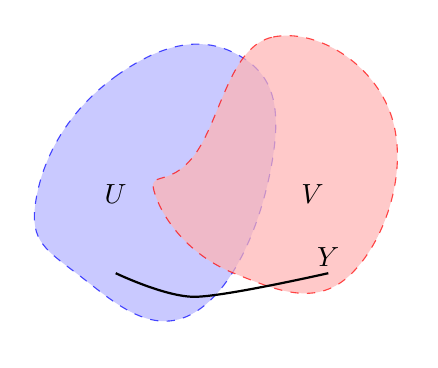
\begin{tikzpicture}
        % First blob using random smooth closed curve
        \draw[dashed, blue, fill=blue!30, opacity=0.7] 
          plot[smooth cycle, tension=0.8] 
          coordinates {(0,0) (1,1.5) (2.5,1.8) (3,0.5) (2,-1.5) (0.5,-1)};

        % Second blob using random smooth closed curve
        \draw[dashed, red, fill=red!30, opacity=0.7] 
          plot[smooth cycle, tension=0.8] 
          coordinates {(2,0.5) (3,2) (4.5,1) (4,-1) (2.5,-1) (1.5,0)};

        % Optional: Add labels
        \node at (1,0) {$U$};
        \node at (3.5,0) {$V$}; 
        \node at (3.7,-0.8) {$Y$}; 
        
        % Horizontal curve
        \draw[thick, -] 
          plot[smooth] coordinates {(1,-1) (2,-1.3) (3.7,-1.0)};
      \end{tikzpicture}
    \caption{We can see that there is a separation of $A = U \cap Y, B = V \cap Y$ of $Y$, but $U$ and $V$ do intersect.} 
  \end{figure}

  Therefore, we cannot rely on the topology on $X$ to deduce connectivity on $Y$. However, there is another simpler lemma that checks for connectivity of subspaces. 

  \begin{lemma}[Closures of One Separated Component is Disjoint from Other]
    If $A, B$ is a separation of subspace $Y \subset X$, then $A^\prime \cap B = \emptyset$ and $A \cap B^\prime = \emptyset$. It immediately follows that 
    \begin{equation}
      \overline{A} \cap B = A \cap \overline{B} = \emptyset
    \end{equation}
  \end{lemma}
  \begin{proof}
    If $A, B$ is a separation, then $A \subset U, B \subset V$ for $U, V$ open in $X$, and $A \cap V = \emptyset, B \cap U = \emptyset$. So points on $B \subset V$ are not limit points of $A$, and same with points on $A$. 
  \end{proof} 

  \begin{lemma}[Connected Subsets Must be Completely Contained in a Separated Component]
    If the sets $C$ and $D$ form a separation of $X$, and if $Y$ is a connected subset of $X$, then $Y$ lies entirely within either $C$ or $D$. 
  \end{lemma}
  \begin{proof}
    We can see that $A = C \cap Y$ and $B = D \cap Y$are open in the subspace topology of $Y$. So $A \cap B = \emptyset$ and $A \cap B = Y$, so either $Y = A$ or $Y = B$. 
  \end{proof}

  Now so far, we have treated connectedness as a property of a space, but we may extend this to talk about whether \textit{points} are connected. Essentially, we want to describe connectedness as an equivalence relation between points. The most nontrivial property is transitivity, which will be established in the following theorem. 

  \begin{theorem}[Points are Connected in a Connected Space]
    Let $X$ be a topological space. Then $X$ is connected iff $\forall x, y \in X$, $\exists$ a connected subspace $A$ s.t. $x, y \in A$. 
  \end{theorem}
  \begin{proof}
    We prove bidirectionally. 
    \begin{enumerate}
      \item $(\rightarrow)$. Take $A = X$. 
      \item $(\leftarrow)$. Let $X = U \cup V$ with $U \cap V = \emptyset$, both nonempty and open. Take $x \in U, y \in V$. So $\exists$ connected $A \subset X$ s.t. $x, y \in A$. But then either $A \subset U$ or $A \subset V$ from the lemma above. Therefore, $X$ is connected by contradiction. 
    \end{enumerate}
  \end{proof}

  Now, we can define connected components as an equivalence class. 

  \begin{corollary}[Connectedness is an Equivalence Relation]
    Let $x \sim_c y$ iff $\exists$ a connected subspace $A \subset X$ s.t. $x, y \in A$. 
  \end{corollary}
  \begin{proof}
    We prove the 3 properties. 
    \begin{enumerate}
      \item \textit{Reflexive}. $x \sim_c x$ clearly since $A = \{x\}$, which is connected. 
      \item \textit{Symmetric}. Let $x \sim_c y$. Then there exists connected subspace $A$ containing both $x, y$, i.e. containing $y, x$, and so $y \sim_c y$. 
      \item \textit{Transitive}. Let $x \sim_c y, y \sim_c z$. Then there exists connected subspaces $A \ni x, y$ and $B \ni y, z$. Since $y \in A \cap B$, $A \cup B$ is also a connected subspace containing $x, z$, and so $x \sim_c z$. 
    \end{enumerate}
  \end{proof}

  \begin{definition}[Connected Components]
    Given a topological space $X$, the equivalence classes under $\sim_c$ are called \textbf{connected components} of $X$. 
  \end{definition}

  With the equivalence class interpretation, it will be much easier to prove many properties. 

\subsection{Constructing Connected Spaces}

  We have proved some pretty basic results, and just like how we have talked about building new topologies from old ones, we can talk about how to build new connected spaces from old connected spaces. The three that we will mention are the unions, limit point extensions, and products. 

\subsubsection{Extensions}

  \begin{theorem}[Conditions for Union of Connected Spaces to be Connected]
    Suppose $A_\alpha \subset X$ are connected subspaces of $X$ s.t. $\forall \alpha, \beta$, $A_\alpha \cap A_\beta = \emptyset$. Then $\cup_\alpha A_\alpha$ is connected. 

  \begin{figure}[H]
    \centering 
    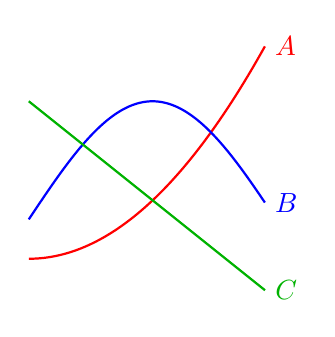
\begin{tikzpicture}
      % Curve A (parabola)
      \draw[thick, red, domain=0:3, samples=100] 
        plot (\x, {0.3*\x*\x - 2}) 
        node[right] {$A$};
        
      % Curve B (sine wave)
      \draw[thick, blue, domain=0:3, samples=100] 
        plot (\x, {1.5*sin(\x r) - 1.5}) 
        node[right] {$B$};
        
      % Curve C (line)
      \draw[thick, green!70!black, domain=0:3] 
        plot (\x, {-0.8*\x}) 
        node[right] {$C$};
    \end{tikzpicture}
    \caption{We can see that the connected subspaces $A, B, C \subset \mathbb{R}^2$ intersect pairwise at a point. Therefore their unions is connected. } 
  \end{figure}

  \end{theorem}
  \begin{proof}
    Let $A = \cup_\alpha A_\alpha$. Suppose $A = C \sqcup D$ with $C, D$ both open in subspace topology, so $C = A \cap U, D = A \cap V$ for $X$-open sets $U, V$. Each $A_\alpha$ is either in $C$ or $D$, since otherwise I can create a separation. But if $A_\alpha \subset C$ or $A_\alpha \subset D$, then this is impossible since they intersect at one point at least. So either all $A_\alpha \subset C$ or all $A_\alpha \subset D$. 
  \end{proof} 

  \begin{theorem}[Connected Sets plus Some/All Limit Points are Connected]
    Let $A$ be a connected subset of $X$. If $A \subset B \subset \bar{A}$, then $B$ is also connected. 
  \end{theorem}
  \begin{proof}
    Assume $B = C \cup D$ is a separation of $B \implies A$ must lie entirely within $C$ or $D$. Without loss of generality, suppose $A \subset C$, which implies that $\bar{A} \subset \bar{C}$. Since $\bar{C}$ and $D$ are disjoint, $B$ cannot intersect $D \implies D = \emptyset$, a contradiction. Therefore, there exists no separation of $B$. 
  \end{proof}

  \begin{theorem}[Products of Connected Spaces are Connected]
    Given connected topological spaces $X_\alpha$ with $\alpha \in J$, the Cartesian product 
    \begin{equation}
      \prod_{\alpha \in J} X_\alpha
    \end{equation}
    under the product topology is connected.\footnote{But for infinite products, it is not necessarily connected under the box topology} 

    \begin{figure}[H]
      \centering 
      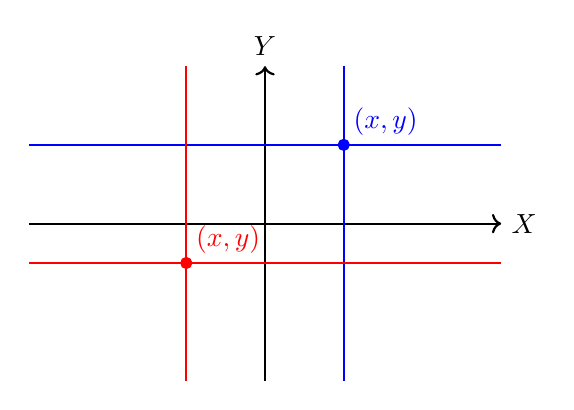
\begin{tikzpicture}
        % Coordinate axes
        \draw[thick, ->] (-3,0) -- (3,0) node[right] {$X$};
        \draw[thick, ->] (0,-2) -- (0,2) node[above] {$Y$};
        
        % Grid lines through point (1,1)
        \draw[blue, thick] (-3,1) -- (3,1) node[right] {};
        \draw[blue, thick] (1,-2) -- (1,2) node[above] {};

        \draw[red, thick] (-3,-0.5) -- (3,-0.5) node[right] {};
        \draw[red, thick] (-1,-2) -- (-1,2) node[above] {};
        
        % Mark the point (1,1)
        \filldraw[blue] (1,1) circle (2pt) node[anchor=south west] {$(x, y)$};
        \filldraw[red] (-1,-0.5) circle (2pt) node[anchor=south west] {$(x, y)$};
      \end{tikzpicture}
      \caption{You can see that any two $T_{x \times y}$ have a nontrivial intersection by construction. This is why we need the $+$ shape.} 
    \end{figure}
  \end{theorem}
  \begin{proof}
    We will prove for the finite product case. Given $(x, y) \in X \times Y$, let us define the space 
    \begin{equation}
      T_{x \times y} \coloneqq (\{x\} \times Y) \cup (X \times \{y\})
    \end{equation}
    where both of the components are connected (since they are homeomorphic to $Y$ and $X$, respectively). We know that $T_{x \times y}$ is connected since it's a union of connected space with nontrivial intersection $(x, y)$, and using the same lemma, the arbitrary union over all points in $X \times Y$ is connected. 
    \begin{equation}
      \bigcup_{(x, y) \in X \times Y} T_{x \times y} = X \times Y
    \end{equation}
    is connected. 
  \end{proof}

  \begin{example}[Connected Components in $\mathbb{R}^n$]
    $\mathbb{R}^n$ is connected, since it's a finite product of $\mathbb{R}$, which we proved was connected. Similarly, all $n$-cells of form $\prod_{i=1}^n (a_i, b_i)$ are also connected as a product of convex sets. 
  \end{example} 

  We will expand on this to prove some already intuitive results. 

  \begin{theorem}
    If $n > 1$, then for any $a \in \mathbb{R}^n$, $\mathbb{R}^n \setminus \{a\}$ is connected. 
  \end{theorem}
  \begin{proof}
    Let $U = \{x \in \mathbb{R}^n \mid x_n > a_n\}$ and $V = \{x \in \mathbb{R}^n \mid x_n < a_n\}$. These are connected since they are of form $\mathbb{R}^{n-1} \times (a, b)$. Now let 
    \begin{align}
      U^\prime & = U \cup \{x \in \mathbb{R}^n \mid x_n = a_n\} \setminus \{a\} \\
      V^\prime & = V \cup \{x \in \mathbb{R}^n \mid x_n = a_n\} \setminus \{a\} 
    \end{align}
    Note that $U^\prime, V^\prime$ are the $U, V$ plus some of its limit points, and so they are connected as well. So $U^\prime \cup V^\prime = \mathbb{R}^n \setminus \{a\}$ connected since they have a nontrivial intersection. 
  \end{proof}

  \begin{corollary}
    $\mathbb{R} \not\cong \mathbb{R}^n$ for $n > 1$. 
  \end{corollary}

\subsubsection{Images of Connected Spaces Under Functions}

  \begin{theorem}[Continuous Images of Connected Spaces are Connected]
    If $X$ is aconnected and $f: X \rightarrow Y$ is continuous, then $f(X)$ is a connected subspace of $Y$. 
  \end{theorem}
  \begin{proof}
    Let $f: X \longrightarrow Y$ be a continuous map, and let $X$ be connected. We wish to prove that the image set $Z = f(X)$ is also connected. Let us denote the restriction of $f$ to $Z$ as
    \begin{equation}
      \Tilde{f}: X \longrightarrow Z
    \end{equation}
    which is continuous and surjective. We prove by contradiction. Assume that $Z = A \cup B$ is a separation of $Z$ into 2 disjoint nonempty open sets. Then, $\Tilde{f}^{-1} (A)$ and $\Tilde{f}^{-1}(B)$ are disjoint open sets whose union is $X \implies \Tilde{f}^{-1} (A) \cup \Tilde{f}^{-1}(B)$ form a separation of $X$. This contradicts the hypothesis that $X$ is connected $\implies Z$ is connected.  
  \end{proof} 

  This establishes the fact that homeomorphisms preserve connectedness, and so connectedness is a topological property.  

  \begin{corollary}[Connectedness is a Topological Property]
    If $X \cong Y$, then $X$ connected iff $Y$ connected. 
  \end{corollary}

  Therefore, connectedness is a good way to prove that two spaces are not homeomorphic, whether it is by assuming a homeomorphism itself or taking the restriction of a homeomorphism with one or more points taken off the domain. 

  \begin{example}[Intervals of Endpoints $0$ and $1$]
    We claim that $(0, 1)$, $[0, 1)$, and $[0, 1]$ are all pairwise not homeomorphic. 
  \end{example}

  \begin{corollary}[Quotient Spaces]
    If $X$ is connected, then any quotient space of $X$ is connected. 
  \end{corollary}

  \begin{example}
    For $n \geq 1$, $S^n$ and $\mathbb{RP}^n$ is connected. 
  \end{example}

  Finally, we conclude with a theorem often seen in calculus, but is really a theorem in topology, since it only relies on continuity rather than derivatives, like the MVT. 

  \begin{theorem}[Intermediate Value Theorem]
    Let $f: X \longrightarrow Y$ be a continuous map of the connected space $X$ into the ordered set $Y$, with the order topology. Given $a, b \in X$ and $r \in Y$ such that $f(a)<r<f(b)$, then there exists a point $c \in X$ such that $f(c) = r$. 
  \end{theorem}
  \begin{proof}
    Assuming the hypothesis, the sets 
    \begin{equation}
      A \equiv f(X) \cap (-\infty, r), \; B \equiv f(X) \cap (r, +\infty)
    \end{equation}
    are disjoint. They are also nonempty since 
    \begin{equation}
      f(a) \in A, \; f(b) \in B
    \end{equation}
    $A$ and $B$ are open since they are the intersection of open sets. Now, assume that there exists no point $c \in X$ such that $f(c) = r$. Then, 
    \begin{equation}
      f(X) = A \cup B
    \end{equation}
    would define a separation of $X$, contradicting the fact that the image of a connected space under a continuous map must be connected. Therefore, $c$ exists. 
  \end{proof}  

\subsection{Path Connectedness} 

  Now we will be talking about a stronger form called path connectedness. Unlike connectedness---where we began with the topological definition and then claimed that the connected components form an equivalence class---we will introduce path connectedness as an equivalence class from the start. Note that connectedness is about open sets rather than paths. 

  \begin{definition}[Path]
    A \textbf{path} from $x \in X$ to $y \in X$ is a continuous function $f: [a, b] \subset \mathbb{R} \rightarrow X$\footnote{Note that we can just reparameterize the path to any other starting and end points with the homeomorphism $[a, b] \cong [c, d$.} s.t. $f(a) = x, f(b) = y$, and $[a, b]$ is endowed with the Euclidean topology.\footnote{So far, we've been pretty agnostic of topologies in definitions, but here we mention a very specific topology.} Two points $x, y$ are said to be \textbf{path connected}, denoted $x \sim_p y$, if there exists a path from $x$ to $y$, i.e. $f(0) = x, f(1) = y$.
  \end{definition} 

  \begin{lemma}[Path Components are Equivalence Classes]
    $\sim_p$ is an equivalence relation, and the equivalence classes formed by $\sim_p$ on topological space $X$ are called \textbf{path components}.  
  \end{lemma}
  \begin{proof}
    We prove the 3 properties. 
    \begin{enumerate}
      \item \textit{Reflexive}. $x \sim_p x$ since we can choose the constant function $f: t \mapsto x$.  
      \item \textit{Symmetric}. Let $x \sim_p y$. Then there exists a continuous $f: [0, 1] \rightarrow X$ s.t. $f(0) = x, f(1) = y$. We can choose the continuous function $g = f \circ h$, where $h(x) = 1 - x$ is continous connecting $y$ to $x$. 
      \item \textit{Transitive}. Let $x \sim_p y$ and $y \sim_p z$. then by the pasting lemma, the overlapping set $\{y\}$ is closed and so we can define the continuous function 
      \begin{equation}
        (f \ast g)(t) \coloneqq \begin{cases} 
          f(2t) & t \in [0, 1/2] \\
          g(2t - 1) & t \in [1/2, 1] 
        \end{cases} 
      \end{equation}
      which is a path from $x$ to $z$. 

      \begin{figure}[H]
        \centering 
        \begin{tikzpicture}
          % Define styles for the endpoints
          \tikzset{
            endpoint/.style={
              circle,
              fill=black,
              inner sep=0pt,
              minimum size=4pt
            }
          }
          
          % First curved line with endpoints
          \node[endpoint] (A) at (1,0) {};
          \node[endpoint] (B) at (4,2) {};
          \draw (A) to[out=50, in=210] (B);
          
          % Second curved line with endpoints
          \node[endpoint] (C) at (4,2) {};
          \node[endpoint] (D) at (6,1) {};
          \draw (C) to[out=20, in=200] (D);
          
          % Labels for the endpoints (optional)
          \node[below left] at (A) {$x$};
          \node[below right] at (B) {$y$};
          \node[above right] at (D) {$z$};
        \end{tikzpicture}
        \caption{W:}
      \end{figure}
    \end{enumerate}
  \end{proof}

  \begin{definition}[Path Connected Space] 
     A topological space $X$ is said to be \textbf{path connected} for every pair of points $x, y \in X$, $x \sim_p y$. 
  \end{definition}

  It seems that path connectedness is conceptually easier to deal with, and we might ask if one implies the other. 

  \begin{theorem}[Path Connectedness implies Connectedness]
    $X$ is path connected $\implies X$ is connected. That is, each path component is contained in a connected component. 

    \begin{figure}[H]
      \centering 
      \begin{tikzpicture}[scale=0.5]
        \draw[dashed] (5,1) circle (2);
        \draw[dashed] (0,0) circle (2);
        \node at (-1,-1) {$C$};
        \node at (6,2) {$D$};
        \draw plot [smooth] coordinates {(0,0) (2,1.5) (4.5,2)};
        \draw[fill] (0,0) circle (0.05);
        \draw[fill] (4.5,2) circle (0.05);
        \node at (-4,1) {$X = C \cup D$};
      \end{tikzpicture}
      \caption{Visually if two spaces are not connected, it doesn't seem like it's path connected. }
      \label{fig:path_vs_reg_connectedness}
    \end{figure}
  \end{theorem}
  \begin{proof} 
    We can prove this in two ways. 
    \begin{enumerate}
      \item \textit{Directly}. if $x \sim_p y$, then $\exists$ a path $f: [0, 1] \rightarrow X$ s.t. $f(a) = x, f(b) = y$, and $\Im(f)$ is a connected subspace containing $x, y$. 

      \item \textit{Contrapositive}. $X$ not connected implies that there exists disjoint open subsets $C, D$ such that $C \cup D = X$. Assume that $X$ is path connected, i.e. there exists a continuous function $g: [0,1] \longrightarrow X$. Then the preimage of $C$ and $D$ in $X$ must be open sets $g^{-1} (C), g^{-1} (D) \subset [0,1]$ such that $g^{-1}(C) \cup g^{-1}(D) = [0,1]$. But this isn't possible since $[0,1]$ is connected, so by contradiction, $X$ is not path connected. The contrapositive of this statement results in the theorem. 
    \end{enumerate}
  \end{proof} 

  But is the converse true? Intuitively, it seems like it, but a pretty nasty construction of a counterexample is needed. 

  However, note that $X$ connected $\centernot\implies$ $X$ path connected. Note the following example. 

  \begin{example}[Topologist's Sine Curve]
    Let 
    \begin{equation}
      C = \{ (x, y) \in \mathbb{R}^2 \mid x > 0, y = \sin(1/x) \}
    \end{equation} 
    This is the image of a continuous function. It is both connected and path connected since $C \cong (0, +\infty)$. This is \textit{not} the topologist's sine curve. $C$ is not closed since it doesn't contain the limit points $\{(0, y) \mid 0 \leq y \leq 1 \}$ (in red), but if we do cake the closure $\overline{C} = C \cup (\{0\} \times [-1, 1])$, then \textit{this} is the TSC. 

    \begin{figure}[H]
      \centering 
      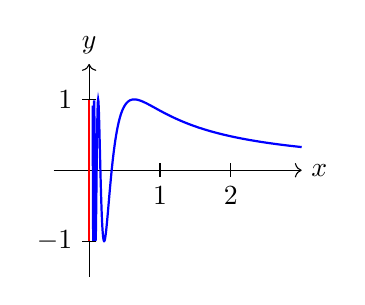
\begin{tikzpicture}[scale=0.9]
        % Draw the coordinate axes
        \draw[->] (-0.5,0) -- (3,0) node[right] {$x$};
        \draw[->] (0,-1.5) -- (0,1.5) node[above] {$y$};
        
        \draw[thick, blue, domain=0.05:3, samples=800, smooth, variable=\x] 
          plot ({\x}, {sin(1/\x r)});
        
        % Add vertical line at x=0
        \draw[dashed] (0,-1.5) -- (0,1.5);
        \draw[red, thick] (0,-1) -- (0,1);
        
        % Mark the x-axis and y-axis
        \foreach \x in {1,2}
          \draw (\x,0.1) -- (\x,-0.1) node[below] {$\x$};
        
        \foreach \y in {-1,1}
          \draw (0.1,\y) -- (-0.1,\y) node[left] {$\y$};
      \end{tikzpicture}
      \caption{Topologist's sine curve is the union of the image of the oscillating sine curve (blue) with its limit points (red).} 
      \label{fig:top_sine_curve}
    \end{figure}

    $\overline{C}$ is connected since the closure is the union of connected $C$ and some/all limit points of $C$. Now we claim that $\overline{C}$ is not path connected. Intuitively, given a point on $C$ and point on $C^\prime$, it must zig-zag infinitely many times, and thus cannot get to the red portion in time. Rigorously, suppose $f: [a, b] \rightarrow \overline{C}$ were a path from $(0, 0)$ to some $(x, y)$ with $x > 0$. $f^{-1} (\{x\} \times [-1, 1])$ is a closed subset of $[a, b]$ and thus has a max value; call it $c$. Now we take the restriction on $f: [c, b] \rightarrow \overline{C}$. Then 
    \begin{equation}
      f(c) \in C^\prime = \{0\} \times [-1, 1], \qquad f(t) \in C \; \forall t > c
    \end{equation} 
    Now reparaterize so that $c = 0, b = 1$. Then 
    \begin{equation}
      f(t) = \big( x(t), y(t) \big) = \big( x(t), \frac{1}{\sin{x(t)}} \big) 
    \end{equation}
    So we can find some sequence of numbers $t_n \rightarrow 0$ s.t. $y(t_n) = (-1)^n \implies \lim_{n \rightarrow +\infty} t_n = 0$ but $\lim_{n \rightarrow +\infty} y(t_n)$ does not exist, contradicting the fact that $f$ is continuous. 
  \end{example} 

  In general, mathematicians like path connectedness better since it makes our lives easier. We can more easily prove path connectedness by just building a path and it also implies connectedness.  

  \begin{example}[Euclidean Space]
    Let us take $\mathbb{R}^n$ and we claim the following. 
    \begin{enumerate}
      \item $\mathbb{R}^n$ is connected since given $x, y$, we can just draw $f(t) = (1 - t) x + ty$ for $t \in [0, 1]$, i.e. a straight line between them. 
      \item $\mathbb{R}^n \setminus \{0\}$ is path connected for $n > 1$ since we can draw a line, and if that line passes through the origin, i.e. $y = \lambda x$ for $lambda < 0$, then we choose $z \not\in \mathrm{span}(x)$ and choose the path $x \rightarrow z \rightarrow y$. 
      \item $\mathbb{R}^n \setminus S$ is path connected for any finite set $S$. 
    \end{enumerate}
  \end{example} 

  \begin{theorem}[Continuous Images of Path Connected Spaces as Path Connected]
    If $X$ is path connected and $f: X \rightarrow Y$ is continuous, then $f(X) \subset Y$ is path connected. 
  \end{theorem}
  \begin{proof}
    Given $y_1, y_2 \in f(X) \subset Y$, we choose $x_1, x_2$ s.t. $f(x_1) = y_1$ and $f(x_2) = y_2$. Then we choose a path $g$ from $x_1$ to $x_2$ since $X$ is path connected, and $f \circ g$ is a path from $y_1$ to $y_2$. 
  \end{proof}

  \begin{corollary}[Path Connectedness is a Topological Property]
    If $X \cong Y$, then $X$ path connected iff $Y$ path connected. 
  \end{corollary}

  \begin{corollary}[Quotients Path Connected Spaces are Path Connected]
    Any quotient of a path connected space is path connected. 
  \end{corollary}

  \begin{theorem}[Products of Path Connected Spaces]
    Any product of path connected spaces is path connected under the product topology.\footnote{Any only for finite products in the box topology.}
  \end{theorem}
  \begin{proof}
    Given $\prod_\alpha X_\alpha$ of path connected components $X_\alpha$, let $x = (x_\alpha), y = (y_\alpha)$ be its elements. Then for each $\alpha$, choose path $f_\alpha: [0, 1] \rightarrow X_\alpha$ with $f_\alpha (0) = x_\alpha$ and $f_\alpha (1) = y_\alpha$. Then by definition of product topology, the function 
    \begin{equation}
      f = \prod_\alpha f_\alpha : [0, 1] \rightarrow \prod_\alpha X_\alpha
    \end{equation}
    is continuous. 
  \end{proof}

  \begin{example}
    $\mathbb{R}^\omega$ is not even connected in the box topology. In fact it is horrifically disconnected. Let 
    \begin{equation}
      B \coloneqq \{x \in \mathbb{R}^\omega \mid |x_i| < R\}
    \end{equation}
    be the set of bounded sequences for some $R > 0$. We claim that $B$ is clopen in the box topology. Given $x \in \mathbb{R}^\omega$, let us define the open set
    \begin{equation}
      U_x = \prod (x_i - 1, x_i + 1) 
    \end{equation}
    If $x$ is bounded, then $x \in B$ and every element in $U_x$ is bounded $\implies U_x \subset B$. So $B$ is open. If $x$ is unbounded, then $x \in \mathbb{R}^\omega \setminus B$ and every element of $U_x$ is also unbounded $\implies U_x \subset \mathbb{R}^\omega \setminus B$. So $\mathbb{R}^\omega \setminus B$ is open and $B$ is closed. 
  \end{example}

\subsection{Local Connectedness and Path Connectedness}

  The property of local connectedness is also important for a space to possess. Roughly speaking, local connectivity means that each point has "arbitrarily small" neighborhoods that are connected. It is a property on small scales, i.e. for a property on open sets. 

  \begin{definition}[Locally (Path) Connected at a Point]
    A space $X$ is said to be \textbf{locally (path) connected at $x$} if for every neighborhood $U$ of $x$, there is a (path) connected open neighborhood $V$ of $x$ contained in $U$. If $X$ is locally (path) connected at all of its points, then $X$ is simply said to be \textbf{locally (path) connected}. 

    \begin{figure}[H]
      \centering 
      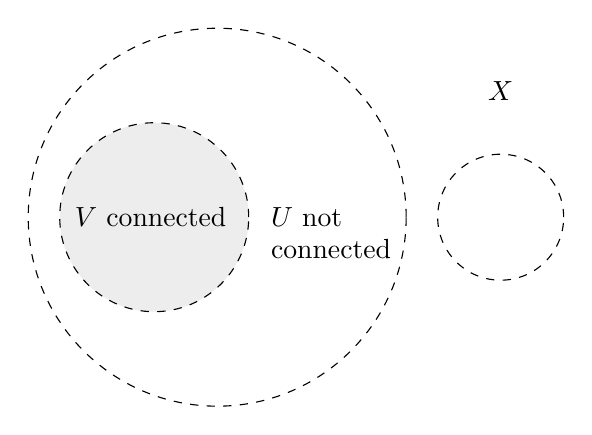
\begin{tikzpicture}[scale=0.8]
        \draw[fill] (-2,0) circle (0.05);
        \node[above] at (-2,0) {$x$};
        \draw[dashed] (-1.5,0) circle (3);
        \draw[dashed] (3,0) circle (1);
        \draw[dashed, fill=lightgray] (-2.5,0) circle (1.5);
        \node[left] at (-1.2,0) {$V$ connected};
        \node[right] at (-0.8,0) {$U$ not};
        \node[right] at (-0.8,-0.5) {connected};
        \node at (3,2) {$X$};
      \end{tikzpicture}
      \caption{Visually, in the space $X$, let $U$ be the union of the two open balls shown below. $U$ is clearly open, but not necessarily connected. However, we can form a  neighborhood $V$ of $x$ contained in $U$ such that $V$ is connected. }
      \label{fig:locally_connected}
    \end{figure}
  \end{definition} 

  \begin{example}[Euclidean Space]
    $\mathbb{R}^n$ plus any open sets in $\mathbb{R}^n$ is locally connected and locally path connected since open balls of any radius are path connected. 
  \end{example} 

  \begin{example}[Topologist's Sine Curve]
    The TSC is not locally connected.  

    \begin{figure}[H]
      \centering 
      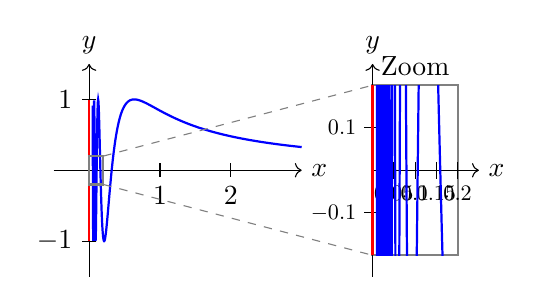
\begin{tikzpicture}[scale=0.9]
        % Draw the coordinate axes
        \draw[->] (-0.5,0) -- (3,0) node[right] {$x$};
        \draw[->] (0,-1.5) -- (0,1.5) node[above] {$y$};
        
        \draw[thick, blue, domain=0.05:3, samples=800, smooth, variable=\x] 
          plot ({\x}, {sin(1/\x r)});
        
        % Add vertical line at x=0
        \draw[dashed] (0,-1.5) -- (0,1.5);
        \draw[red, thick] (0,-1) -- (0,1);
        
        % Mark the x-axis and y-axis
        \foreach \x in {1,2}
          \draw (\x,0.1) -- (\x,-0.1) node[below] {$\x$};
        
        \foreach \y in {-1,1}
          \draw (0.1,\y) -- (-0.1,\y) node[left] {$\y$};
          
        % Add zoom box
        \draw[gray, thick] (0,-0.2) rectangle (0.2,0.2);
        
        % Draw the zoomed area
        \begin{scope}[shift={(4,0)}, scale=6]
          % Box outline
          \draw[gray, thick] (0,-0.2) rectangle (0.2,0.2);
          \node[above] at (0.1,0.2) {Zoom};
          
          % Axes for zoomed region
          \draw[->] (0,0) -- (0.25,0) node[right] {$x$};
          \draw[->] (0,-0.25) -- (0,0.25) node[above] {$y$};
          
          % Labels for x-axis in zoomed region
          \draw (0.05,0.02) -- (0.05,-0.02) node[below, scale=0.8] {$0.05$};
          \draw (0.1,0.02) -- (0.1,-0.02) node[below, scale=0.8] {$0.1$};
          \draw (0.15,0.02) -- (0.15,-0.02) node[below, scale=0.8] {$0.15$};
          \draw (0.2,0.02) -- (0.2,-0.02) node[below, scale=0.8] {$0.2$};
          
          % Labels for y-axis in zoomed region
          \draw (0.02,0.1) -- (-0.02,0.1) node[left, scale=0.8] {$0.1$};
          \draw (0.02,-0.1) -- (-0.02,-0.1) node[left, scale=0.8] {$-0.1$};
          
          % Clip the function in the zoomed area to stay within y = -0.2 to 0.2
          \begin{scope}
            \clip (0,-0.2) rectangle (0.2,0.2);
            \draw[thick, blue, domain=0.01:0.2, samples=1500, smooth, variable=\x] 
              plot ({\x}, {sin(1/\x r)});
          \end{scope}
          
          % Add vertical line at x=0 in zoomed region
          \draw[red, thick] (0,-0.2) -- (0,0.2);
        \end{scope}
        
        % Add connector lines between the boxes
        \draw[gray, dashed] (0.2,0.2) -- (4,1.2);
        \draw[gray, dashed] (0.2,-0.2) -- (4,-1.2);
      \end{tikzpicture}
      \caption{If we take a neighborhood around $(0, 0)$, we can see that the intersection of the image of a function with the open ball around the origin will consists of many almost-vertical lines that are not connected.} 
      \label{fig:top_sine_curve_2}
    \end{figure}
  \end{example}

  Even though local properties alone does not in general allow us to conclude about a global property, there are times when it does. 

  \begin{theorem}[LPC + C $\implies$ PC]
    If $X$ is locally path connected, connectedness $\iff$ path connectedness, i.e. the connected components and path connected components are the same. In other words, 
    \begin{equation}
      \text{Local Path Connectedness } + \text{ Connectedness} \implies \text{ Path Connectedness}
    \end{equation}
  \end{theorem} 

  Equivalently, $X$ is locally connected if there exists a basis for $X$ consisting of connected sets. Local connectedness and connectedness of a space are independent of each other. 

  \begin{theorem}[Open Components and Local (Path) Connectedness]
    Given space $X$, 
    \begin{enumerate}
      \item $X$ is locally connected iff its connected components are open. 
      \item $X$ is locally path connected if its path connected components are open. 
    \end{enumerate}
  \end{theorem}
  \begin{proof}
    For the first claim, we prove bidirectionally. 
    \begin{enumerate}
      \item $(\rightarrow)$ Suppose that $X$ is locally connected. Let $U$ be an open set of $X$ and let $C$ be a component of $U$. If $x$ is any point in $C$, by definition of local connectedness, there exists a connected neighborhood $V$ of $x$ fully contained in $U$. Since $V$ is connected, it must additionally lie completely within $C \implies C$ is open in $X$. 
      \item $(\leftarrow)$ Suppose that the components of open sets in $X$ are open. Given a point $x \in X$ and neighborhood $U$ of $x$, let $C$ be the component of $U$ containing $x$, which means that $C$ is connected. By hypothesis, the components of open sets are alsvo open, so $C$ is also open. Since an open, connected set $C$ exists for all $x \in X$, $X$ is locally connected. 
    \end{enumerate}
    For the second claim, we also prove bidirectionally. 
    \begin{enumerate}
      \item TBD. 
      \item TBD. 
    \end{enumerate}
  \end{proof}

\subsection{Homotopies}

  The concept of homotopies is dealt with in algebraic topology, but it is worthwhile to mention it now. 

  \begin{definition}[Homotopy]
    Two continuous paths from $x$ to $y$ in topological space $X$ is \textbf{homotopic} if one can be continuously "deformed" into the other, such a deformation being the \textbf{homotopy} between two functions. The set of linearly homotopic paths form a relation, and thus \textbf{homotopy classes} can be further defined. 
    \begin{figure}[H]
      \centering 
      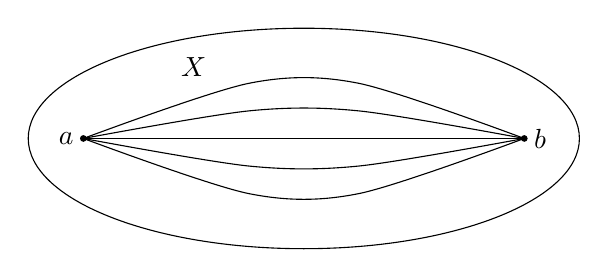
\begin{tikzpicture}[scale=0.7]
        \draw (0,0) ellipse (5 and 2);
        \draw[fill] (-4,0) circle (0.05);
        \draw[fill] (4,0) circle (0.05);
        \draw plot [smooth] coordinates {(-4,0) (-1,1) (1,1) (4,0)};
        \draw (-4,0)--(4,0);
        \draw plot [smooth] coordinates {(-4,0) (-1,0.5) (1,0.5) (4,0)};
        \draw plot [smooth] coordinates {(-4,0) (-1,-0.5) (1,-0.5) (4,0)};
        \draw plot [smooth] coordinates {(-4,0) (-1,-1) (1,-1) (4,0)};
        \node at (-2,1.3) {$X$};
        \node[left] at (-4,0) {$a$};
        \node[right] at (4,0) {$b$};
      \end{tikzpicture}
      \caption{Visually, the set of all the curves in the space $X$ as shown are in a single homotopy class.} 
      \label{fig:single_homotopy_class}
    \end{figure}
  \end{definition}

  It is clear that the space $X$ consists of a single homotopy class of curves from $a$ to $b$. However, a space may have an infinite number of such classes. 

  \begin{figure}[H]
    \centering 
    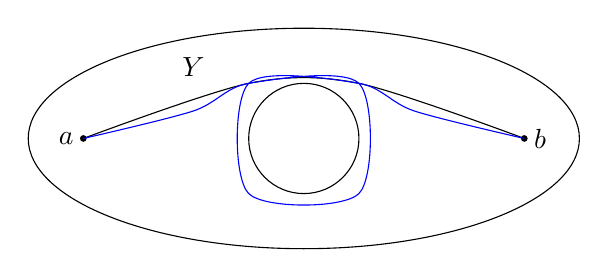
\begin{tikzpicture}[scale=0.7]
      \draw (0,0) ellipse (5 and 2);
      \draw[fill] (-4,0) circle (0.05);
      \draw[fill] (4,0) circle (0.05);
      \draw plot [smooth] coordinates {(-4,0) (-1,1) (1,1) (4,0)};
      \node[left] at (-4,0) {$a$};
      \node[right] at (4,0) {$b$};
      \draw (0,0) circle (1);
      \node at (-2,1.3) {$Y$};
      \draw[blue] plot [smooth] coordinates {(-4,0) (-2,0.5) (-1,1) (1,1) (1,-1) (-1,-1) (-1,1) (1,1) (2,0.5) (4,0)};
    \end{tikzpicture}
    \caption{Let us define the space $Y \equiv X \setminus C$ where $C$ is a circular region in $X$. Then, $Y$ has an infinite number of homotopy classes. We show two curves, that are in two different homotopy classes. }
    \label{fig:homotopy_class}
  \end{figure}

  \begin{definition}[Simply Connected Set]
    A \textbf{simply connected set} is a set such that all paths between any two given points are homotopic. That is, a simply connected set has one homotopy class. 
  \end{definition}



\section{Compactness}

  \begin{definition}[Covers]
    A collection $\C$ of subsets of a space $X$ is said to \textbf{cover} $X$, or to be a \textbf{covering} of $X$, if the union of the elements of $\C$ is equal to $X$. It is called an \textbf{open covering} of $X$ if its elements are open subsets of $X$. 
  \end{definition}

  \begin{definition}[Compactness]
    A space $X$ is said to be \textbf{compact} if every open covering of $X$ contains a finite subcovering (i.e. a finite collection of subcovers) of $X$. It may be better to think of compactness as such: If you can find any infinite open covering of the space, then it is not compact. 
  \end{definition}

  \begin{lemma}
    Let $Y$ be a subspace of $X$. Then $Y$ is compact if and only if every covering of $Y$ by sets open in $X$ contains a finite subcollection covering $Y$. 
  \end{lemma}


  \begin{example}[Open Square is Not Compact]
    The subset $Y \equiv (0,1) \times (0,1) \subset \mathbb{R}^2$ is not compact. That is, we can choose to cover the subspace by the finite union of open sets. 
    \begin{equation}
      [0,1]^2 \subset \bigcup_{k=0}^\infty \Big( \frac{2^k - 1}{2^k}, \frac{2^{k+1} - 1}{2^{k+1}} \Big) \times (0,1)
    \end{equation}

    \begin{figure}[H]
      \centering 
      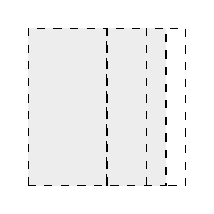
\begin{tikzpicture}[scale=2]
        \draw[dashed] (0,0) rectangle (1,1);
        \draw[dashed, fill=lightgray] (0,0) rectangle (0.5,1);
        \draw[dashed, fill=lightgray] (0.5,0) rectangle (0.75,1);
        \draw[dashed, fill=lightgray] (0.75,0) rectangle (0.875,1);
      \end{tikzpicture}
      \caption{We show the first three elements of the infinite union that covers the open square. }
      \label{fig:closed_square_compact}
    \end{figure}
    \begin{center}
    \end{center}
  \end{example}

  \begin{theorem}
    Every closed subset of a compact space is compact. 
  \end{theorem}
  \begin{proof}
    This proof is quite trivial. Let $Y$ be a closed subset of compact space $X$. Given a covering $\mathcal{C}$ of $Y$ by sets open in $X$, let us form an open covering $\B$ of $X$ by adjoining to $\mathcal{C}$ the single open set $X \setminus Y$. Then, we an see that both $\B$ and $\mathcal{C} \cup (X \setminus Y)$ covers $X$. 
    \begin{equation}
      \B = \mathcal{C} \cup (X \setminus Y)
    \end{equation}
    Since $\B$ is finite, the right hand side must also be expressible as a finite union. Looking through $\B$, we can throw away all the open sets that are entirely in $X \setminus Y$. What remains is a finite covering of $Y$. 
  \end{proof}

  \begin{theorem}
    Every compact subset of a Hausdorff space is closed. 
  \end{theorem}
  \begin{proof}
    Let $Y$ be a compact subset of the Hausdorff Space $X$. We claim that $X \setminus Y$ is open. Let $x \in X \setminus Y$. Then, for each point $y_i \in Y$, we can choose disjoint neighborhoods $U_i$ of $x$ and $V_i$ of $y_i$ (using the Hausdorff condition). The collection 
    \begin{equation}
      \{V_i \; | \; y_i \in Y\}
    \end{equation}
    is an open covering $Y$. Since $Y$ is compact, there must exist a finite number of open sets $V_1, V_2, \ldots , V_n$ covering $Y$. Therefore, 
    \begin{equation}
      \bigcup_{i=1}^n V_i
    \end{equation}
    contains $Y$ and is disjoint from the intersection of open neighborhoods of $x$
    \begin{equation}
      U \equiv \bigcap_{i=1}^n U_i
    \end{equation}
    Therfore, $U$ is an open neighborhood of $x_0$, disjoint from $Y \implies X \setminus Y$ is open $\implies Y$ is closed.
  \end{proof}

  This results gives the following lemma. 

  \begin{lemma}
    If $Y$ is a compact subset of a Hausdorff space $X$ and $x$ is not in $Y$, then there exist disjoint open sets $U$ and $V$ of $X$ containing $x$ and $Y$, respectively. 

    \begin{figure}[H]
      \centering 
      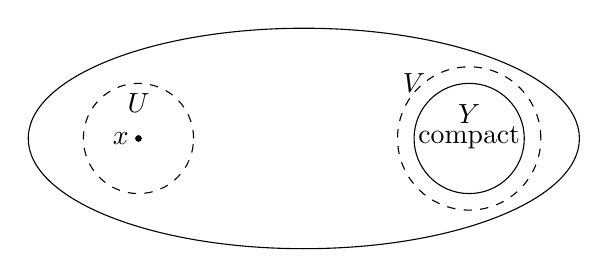
\begin{tikzpicture}[scale=0.7]
        \draw (0,0) ellipse (5 and 2);
        \draw[dashed] (-3,0) circle (1);
        \draw[fill] (-3,0) circle (0.05);
        \node[left] at (-3,0) {$x$};
        \draw (3,0) circle (1); 
        \node[below] at (3,0.8){$Y$};
        \node[below] at (3, 0.4){compact};
        \node[above] at (-3,0.3) {$U$};
        \draw[dashed] (3,0) circle (1.3); 
        \node at (2,1) {$V$};
      \end{tikzpicture}
      \label{fig:hausdorff_compact}
    \end{figure}
  \end{lemma}


  \begin{theorem}
    The image of a compact space under a continuous map is compact.
  \end{theorem}
  \begin{proof}
    Let $f: X \rightarrow Y$ be continuous, and let $X$ be compact. Let $\mathcal{C}$ be a covering of the set $f(X)$ by sets open in $Y$. Then, the preimage of these sets is the collection
    \begin{equation}
      \{f^{-1}(\mathcal{A}) \; | \; \mathcal{A} \in \mathcal{C}\}
    \end{equation}
    which clearly covers $X$. But since $X$ is compact, a finite number of them, say
    \begin{equation}
      f^{-1} (\mathcal{A}_1), f^{-1} (\mathcal{A}_2), \ldots , f^{-1} (\mathcal{A}_n)
    \end{equation}
    covers $X \implies \mathcal{A}_1, \mathcal{A}_2, \ldots, \mathcal{A}_n$ covers $f(X)$. 
  \end{proof}

  \begin{theorem}
    Let $f: X \rightarrow Y$ be a bijective continuous function. If $X$ is compact and $Y$ is Hausdorff, then $f$ is a homeomorphism. 
  \end{theorem}
  \begin{proof}
    It suffices to prove that $f$ is an open or closed mapping. We shall show that $f$ is the latter. Let $U$ be closed in $X$. By the previous theorems, $U$ is compact $\implies f(U)$ is compact in Hausdorff $Y \implies f(U)$ is closed. Therefore, $f$ is closed. 
  \end{proof}

  We now introduce a useful lemma that will come around in many future cases. 

  \begin{lemma}[Tube Lemma]
    Consider the product space $X \times Y$, where $Y$ is compact. If $N$ is an open set $X \times Y$ containing the slice $x_0 \times Y$ of $X \times Y$, then $N$ contains some tube $W \times Y$ about $x_0 \times Y$, where $W$ is a neighborhood of $x_0$ in $X$. 

    \begin{figure}[H]
      \centering 
      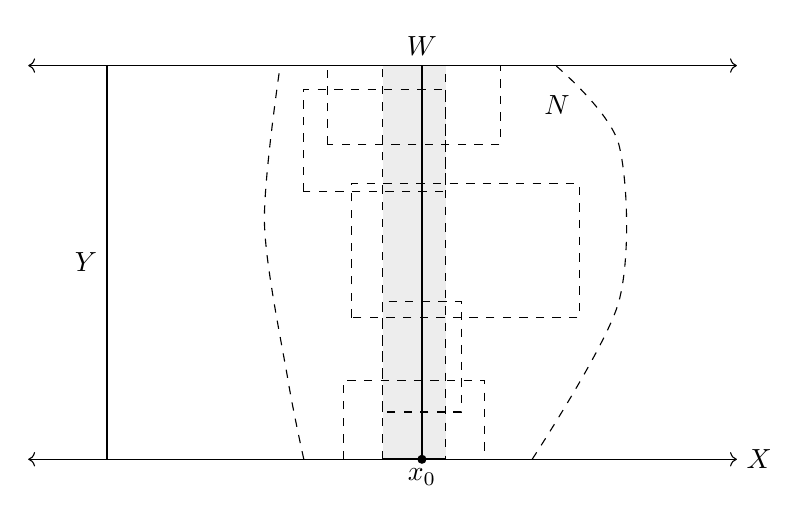
\begin{tikzpicture}
        \draw[dashed, fill=lightgray] (3.5,0) rectangle (4.3,5);
        \draw (0,0)--(0,5);
        \draw[<->] (-1,0)--(8,0);
        \node[right] at (8,0) {$X$};
        \node[left] at (0,2.5) {$Y$};
        \draw[<->] (-1,5)--(8,5);
        \draw[thick] (4,0)--(4,5);
        \draw[dashed] (3,0) rectangle (4.8,1);
        \draw[dashed] (3.5,0.6) rectangle (4.5,2);
        \draw[dashed] (3.1,1.8) rectangle (6,3.5);
        \draw[dashed] (2.5,3.4) rectangle (4.3,4.7);
        \draw[dashed] (2.8,4) rectangle (5, 5);
        \draw[thick] (3.5,0)--(4.3,0);
        \node[above] at (4,5) {$W$};
        \node[below] at (4,0) {$x_0$};
        \draw[fill] (4,0) circle (0.05);
        \draw[dashed] plot [smooth] coordinates {(2.5,0) (2.3, 1) (2,3) (2.2,5)};
        \draw[dashed] plot [smooth] coordinates {(5.4,0) (6.5,2) (6.5,4) (5.7,5)};
        \node[left] at (6,4.5) {$N$};
      \end{tikzpicture}
      \label{fig:tube_lemma}
    \end{figure}
  \end{lemma}
  \begin{proof}
    Let us cover $x_0 \times Y$ by basis elements $U \times V$ (for the topology of $X \times Y$) lying in $N$. The space $x_0$ is compact since it is homeomorphic to $Y \implies$ we can cover $x_0 \times Y$ by finitely such basis elements
    \begin{equation}
      U_1 \times V_1, U_2 \times V_2, \ldots , U_n \times V_n
    \end{equation}
    Without loss of generality, we can assume that each $U_i \times V_i$ has a nontrivial intersection with $x_0 \times Y$, since otherwise, it would be superfluous. Now, we define the intersection of all the open neighborhoods of $x_0$ in $X$ of the basis elements $U_i \times V_i$. That is, let
    \begin{equation}
      W \equiv \bigcup_{i=1}^n U_i
    \end{equation}
    As an intersection of open sets, $W$ is also open containing $x_0$. With this well-defined tube $W \times Y$, we claim that it is entirely contained within $N$. That is, given a point $x \times y \in W \times Y$, consider the corresponding point $x_0 \times y$ that is the image of the projection of $x\times y$ onto $x_0 \times Y$. Clearly, $x_0 \times y$ belongs to some $U_k \times V_k$ (for some $k$) $\implies y \in V_k$. Since $x \in W$, $x$ is clearly in $U_k$, meaning that $x \times y \in U_k \times V_k \subset N$, as desired. 
  \end{proof}

  \begin{theorem}
    The product of finitely many compact spaces is compact. 
  \end{theorem}
  \begin{proof}
    Using induction, it suffices to prove that the product of 2 compact spaces is compact. Let $X$ and $Y$ be compact spaces. By the tube lemma, for each $x \in X$, there exists a neighborhood $W_x$ of $x$ such that the tube $W_x \times Y$ can be covered with finitely (by compactness of $Y$) many open sets in $X \times Y$. The collection of all neighborhoods $W_x$ is an open covering of $X$. By compactness of $X$, there exists a finite subcollection
    \begin{equation}
      W_1, W_2, \ldots , W_k
    \end{equation}
    covering $X$. The finite union of the tubes 
    \begin{equation}
      \bigcup_{i=1}^k W_i \times Y
    \end{equation}
    clearly covers $X \times Y$, meaning that $X \times Y$ is compact. 
  \end{proof}

  \begin{definition}[Finite Intersection Condition]
    A collection $\mathcal{C}$ of subsets of $X$ is said to satisfy the \textbf{finite intersection condition} if for every finite subcollection 
    \begin{equation}
      \{\mathcal{C}_1, \mathcal{C}_2, \ldots , \mathcal{C}_n\}
    \end{equation}
    of $\mathcal{C}$, the intersection
    \begin{equation}
      \bigcap_{i=1}^n \mathcal{C}_i
    \end{equation}
    is nonempty. 
  \end{definition}

  Clearly, the empty sets cannot below to any collection with the finite intersection property. Additionally, the condition is trivially satisfied if the intersection over the entire collection is non-empty or if the collection is nested. However, here is one example that does satisfy the finite intersection condition. 

  \begin{example}
    Let $X = (0,1)$ and for each positive integer $i$, $X_i$ is the set of elements of $X$ having a decimal expansion with digit $0$ in the $i$th decimal place. Then, any finite intersection of $X_i$'s is nonempty, but the intersection of all $X_i$ for $i \in \mathbb{N}$ is empty, since no element of $(0,1)$ has all zero digits. 
  \end{example}

  Here is an analogous example to the previous one. 

  \begin{example}
    In the space $\mathbb{R}$, let us define $C_i \equiv \mathbb{R} \setminus \{i\}$. That is, $C_i$ is $\mathbb{R}$ missing a point at $i$. Then, the collection of all $C_i$'s does satisfy the finite intersection condition. We show below the finite intersection of the five subsets $C_0, C_1, C_2, C_3, C_4$. 

    \begin{figure}[H]
      \centering 
      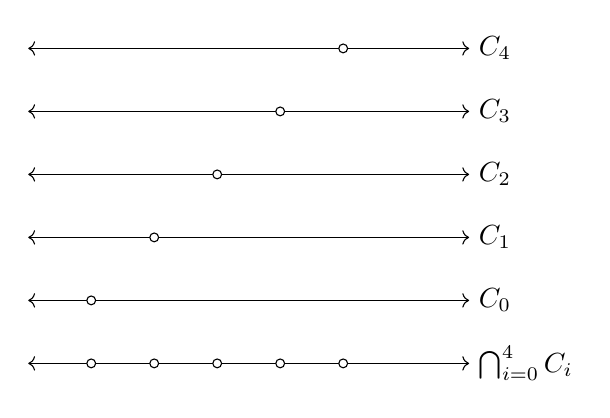
\begin{tikzpicture}[scale=0.8]
        \draw[<->] (-1,0)--(6,0);
        \draw[<->] (-1,1)--(6,1);
        \draw[<->] (-1,2)--(6,2);
        \draw[<->] (-1,3)--(6,3);
        \draw[<->] (-1,4)--(6,4);
        \draw[<->] (-1,-1)--(6,-1);
        \draw[fill=white] (0,0) circle (0.07); 
        \draw[fill=white] (1,1) circle (0.07); 
        \draw[fill=white] (2,2) circle (0.07); 
        \draw[fill=white] (3,3) circle (0.07); 
        \draw[fill=white] (4,4) circle (0.07); 
        \draw[fill=white] (0,-1) circle (0.07); 
        \draw[fill=white] (1,-1) circle (0.07); 
        \draw[fill=white] (2,-1) circle (0.07); 
        \draw[fill=white] (3,-1) circle (0.07); 
        \draw[fill=white] (4,-1) circle (0.07); 
        \node[right] at (6,-1) {$\bigcap_{i=0}^4 C_i$};
        \node[right] at (6,0) {$C_0$};
        \node[right] at (6,1) {$C_1$};
        \node[right] at (6,2) {$C_2$};
        \node[right] at (6,3) {$C_3$};
        \node[right] at (6,4) {$C_4$};
      \end{tikzpicture}
      \label{fig:ex}
    \end{figure}
  \end{example}


  \begin{theorem}
    Let $X$ be a topological space. Then $x$ is compact if and only if for any collection $\mathcal{C}$ of closed sets in $X$ satisfying the finite intersection condition, the intersection 
    \begin{equation}
      \bigcap_{C \in \mathcal{C}} C
    \end{equation}
    of all the elements of $\mathcal{C}$ is nonempty. 
  \end{theorem}
  \begin{proof}
    Given a collection $S$ fo subets of $X$, let 
    \begin{equation}
      \mathcal{C} \equiv \{X \setminus A \; | \; A \in S\}
    \end{equation}
    be the collection of their complements. Then, the following statements hold 
    \begin{enumerate}
      \item $S$ is a collection of open sets if and only if $\mathcal{C}$ is a collection of closed sets. 
      \item The collection $S$ covers $X$ if and only if the intersection 
      \begin{equation}
        \bigcap_{C \in \mathcal{C}} C
      \end{equation}
      of all the elements of $\mathcal{C}$ is empty. 

      \item The finite subcollection $\{A_1, A_2, \ldots , A_n\}$ of $S$ covers $X$ if and only if the intersection of the corresponding elements $C_i \equiv X \setminus A$ of $\mathcal{C}$ is empty. 
    \end{enumerate}
    Clearly, (1) is trivial, and (2) and (3) follows from DeMorgan's Law. 
    \begin{equation}
      X \setminus \bigcup_{\alpha \in J} A_\alpha = \bigcap_{\alpha \in J} (X \setminus A_\alpha)
    \end{equation}
    Using statement 3, the existence of a finite collection of closed sets $C$ in $X$ satisfying the finite intersection condition is equivalent to its complements (which are open sets) covering $X$, which is precisely the definition of compactness. 
  \end{proof}

  Clearly, the previous example in the real line $\mathbb{R}$ shows that $\mathbb{R}$ is indeed not compact. 

  \begin{corollary}
    The space $X$ is compact if and only if every collection $\C$ of subsets of $X$ satisfying the finite intersection condition, the intersection 
    \begin{equation}
      \bigcap_{A \in \C} \bar{A}
    \end{equation}
    of their closures is nonempty. 
  \end{corollary}

\subsection{Compact Sets of the Real Line}

  In order to construct new compact spaces from old ones, we must prove compactness for a number of fundamental spaces. The real number line is a good starting point, and in order to prove that every closed interval in $\mathbb{R}$ is compact, we only need the following theorem. 

  \begin{theorem}
    Let $X$ be a simply ordered set having the least upper bound property (That is, every nonempty subset of $X$ with an upper bound has a least upper bound). Then, in the order topology, every closed interval in $X$ is compact. 
  \end{theorem}

  \begin{corollary}
    Every closed interval in $\mathbb{R}$ is compact. 
  \end{corollary}

  \begin{theorem}[Heine-Borel Theorem]
    A subset $A$ of $\mathbb{R}^n$ is compact if and only if it is closed and bounded in the Euclidean metric $d$ or the square metric $p$. 
  \end{theorem}

  \begin{example}
    The unit sphere $S^{n-1}$ and the closed ball $B^n$ in $\mathbb{R}^n$ are compact since they are closed and bounded. The set
    \begin{equation}
      A \equiv \{(x, \frac{1}{x}) \; | \; 0 < x \leq 1\}
    \end{equation}
    is closed in $\mathbb{R}^2$, but is not compact since it is not bounded. The set 
    \begin{equation}
      S \equiv \{(x, \sin{\frac{1}{x}}) \; | \; 0<x\leq 1\}
    \end{equation}
    is bounded in $\mathbb{R}^2$, but it is not compact since it is not closed. 
  \end{example}

  \begin{theorem}[Maximum, Minimum Value Theorem]
    Let $f: X \rightarrow Y$ be continuous, where $Y$ is an ordered set in the order topology. If $X$ is compact, then there exists points $c$ and $d$ in $X$ such that $f(c) \leq f(x) \leq f(d)$ for every $x \in X$. That is, $f$ has a maximum and a minimum at the values $d$ and $c$, respectively. 
  \end{theorem}

\subsection{Limit Point Compactness}

  We now state different, weaker types of compactness. 

  \begin{definition}[Sequentially Compact]
    A space $X$ is said to be \textbf{sequentially compact} if every sequence of points in $X$ has a subsequence that converges to a point $x \in X$. 
  \end{definition}

  \begin{definition}[Countably Compact]
    A space $X$ is said to be \textbf{countably compact} if every countably open cover has a finite subcover. 
  \end{definition}

  \begin{definition}[Limit Point Compactness]
    A space $X$ is said to be \textbf{limit point compact} if every infinite subset of $X$ has a limit point. 
  \end{definition}

  \begin{theorem}
    Compactness $\implies$ limit point compactness.  
  \end{theorem}

  \begin{lemma}[Lebesgue Number Lemma]
    Let $\C$ be an open covering of the metric space $(X, d)$. If $X$ is compact, then there is a $\delta > 0$ such that for each subset of $X$ having diameter than $\delta$, there exists an element of $\C$ containing it. This number $\delta$ is called a \textbf{Lebesgue number} for the covering $\C$. 
  \end{lemma}

  Another theorem of calculus, suitably generalized to topological spaces, is stated. 

  \begin{theorem}[Uniform Continuity Theorem]
    Let $f: X \rightarrow Y$ be a continuous map of the compact metric space $(X,d_X)$ to the metric space $(Y, d_Y$. Then, $f$ is uniformly continuous. That is, given $\epsilon > 0$, there exists a $\delta > 0$ such that for any two points $x_1, x_2 \in X$, 
    \begin{equation}
      d_X (x_1, x_2) < \delta \implies d_Y \big( f(x_1), f(x_2)\big) < \epsilon
    \end{equation}
  \end{theorem}

  \begin{theorem}[Equivalence of Compactness in Metrizable Spaces]
    Let $(X, \T)$ be a metrizable space. Then the following are equivalent: 
    \begin{enumerate}
      \item $X$ is compact. 
      \item $X$ is limit point compact. 
      \item $X$ is sequentially compact. 
      \item $X$ is countably compact. 
    \end{enumerate}
  \end{theorem}

\subsection{Local Compactness}

  \begin{definition}[Locally Compact]
    A space $X$ is said to be \textbf{locally compact} at $x$ if there is some compact subset $C$ of $X$ that contains a neighborhood of $x$. If $X$ is locally compact at each of its points, $X$ is simply to be \textbf{locally compact}. 
  \end{definition}

  \begin{example}
    The real line $\mathbb{R}$ is locally compact since any point $x \in \mathbb{R}$ lies within a certain closed interval $[a,b]$, which is compact. The subspace $\mathbb{Q}$ is not locally compact. 
  \end{example}

  Two of the most well-behaved classes of spcaes to deal with are metrizable spaces and compact Hausdorff spaces. If a given space is not one of these types, the next best thing one can hope for is that it is a subspace of one of these spaces. Clearly, a subspace of a metrizable space is itself metrizable, so one does not get any new spaces this way. However, a subspace of a compact Hausdorff space need not be compact. This leads to the question: Under what conditions is a space homeomorphic to a subspace of a compact Hausdorff space? 

  \begin{definition}[Compactification]
    Let $X$ be a locally compact Hausdorff space. Take some object outside $X$, denoted by the symbol $\infty$, and adjoin it to $X$, forming the set
    \begin{equation}
      Y = X \cup \{\infty\}
    \end{equation}
    Topologize $Y$ by defining the collection of open sets in $Y$ to be the sets of the following types:
    \begin{enumerate}
      \item $U$, where $U$ is an open subset of $X$. 
      \item $Y \setminus C$, where $C$ is a compact subset of $X$.
    \end{enumerate}
    Then, this space $Y$ is called the \textbf{one-point compactification of $X$}. This is in some sense the minimal compactification of $X$. 
  \end{definition}

  We briefly show that this set of open sets on $Y$ is indeed a topology. First, $\emptyset$ is of type 1 and $Y$ itself is of type 2. Given $U_i$ of type 1 and $Y \setminus C_i$ of type 2, we have the intersections of two sets
  \begin{align*}
    &U_1 \cap U_2 & \text{ is type 1} \\
    &(Y \setminus C_1) \cap (Y \setminus C_2) = Y \setminus (C_1 \cup C_2) & \text{ is type 2} \\
    &U_1 \cap (Y \setminus C_1) = U_1 \cap (X \setminus C_1) & \text{ is type 1} 
  \end{align*}
  along with the arbitrary union of sets
  \begin{align*}
    &\bigcup U_\alpha = U & \text{ is type 1} \\
    &\bigcup (Y \setminus C_\beta) = Y \setminus (\bigcap C_\beta) = Y \setminus C & \text{ is type 2} \\
    &(\bigcup U_\alpha) \cup ( \bigcup (Y \setminus C_\beta)) = U \cup (Y \setminus C) = Y \setminus (C \setminus U) & \text{ is type 2}
  \end{align*}
  We now present some properties of one-point compactifications. 

  \begin{theorem}
    Let $X$ be a locally compact Hausdorff space which is not compact, and let $Y$ be a one-point compactification of $X$. Then $Y$ is a compact Hausdorff space. Additionally, since $X \subset Y$ with $Y \setminus X$ consisting of a single point, $\bar{X} = Y$. 
  \end{theorem}

  \begin{example}[Extended Real Number Line]
    The one-point compactification of the real line $\mathbb{R}$ is homeomorphic to the circle $S^1$. That is, 
    \begin{equation}
      \mathbb{R} \cup \{\infty\} \cong S^1
    \end{equation}
    $\mathbb{R} \cup \{\infty\}$ is called the \textbf{extended real number line}. 
    
    \begin{figure}[H]
      \centering 
      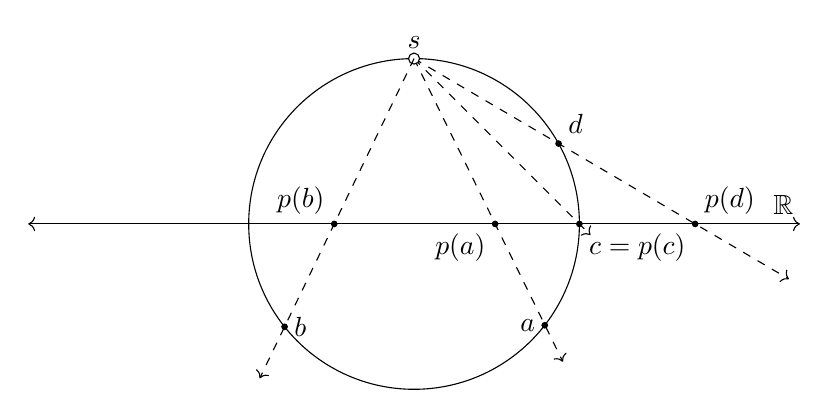
\begin{tikzpicture}[scale=0.7]
        \draw (0,0) circle (3);
        \node[above] at (0,3) {$s$};
        \draw[<->] (-7,0)--(7,0);
        \node[above] at (6.7,0) {$\mathbb{R}$};
        \draw[->, dashed] (0,3)--(3.2,-0.2);
        \draw[->, dashed] (0,3)--(2.7,-2.5);
        \draw[->, dashed] (0,3)--(6.8,-1);
        \draw[fill=white] (0,3) circle (0.1);
        \draw[->, dashed] (0,3)--(-2.8, -2.8);
        \draw[fill] (3,0) circle (0.05);
        \draw[fill] (-2.349,-1.866) circle (0.05);
        \draw[fill] (5.1,0) circle (0.05);
        \draw[fill] (2.622,1.458) circle (0.05);
        \draw[fill] (-1.448,0) circle (0.05);
        \draw[fill] (1.471,0) circle (0.05); 
        \draw[fill] (2.371, -1.838) circle (0.05);
        \node[left] at (2.371, -1.838) {$a$};
        \node[below left] at (1.471,0) {$p(a)$};
        \node[above left] at (-1.448,0) {$p(b)$};
        \node[right] at (-2.349,-1.866) {$b$};
        \node[above right] at (5.1,0) {$p(d)$};
        \node[above right] at (2.622,1.458) {$d$};
        \node[below right] at (3,0) {$c = p(c)$};
      \end{tikzpicture}
      \caption{We can visualize this homeomorphism by visualizing the stereographic projection $p: S^1 \setminus \{s\} \rightarrow \mathbb{R}$. } 
      \label{fig:extended_r}
    \end{figure}
  \end{example}

  \begin{example}[2-Sphere]
    The one point-compactification of the real plane $\mathbb{R}^2$ is homeomorphic to the 2-sphere $S^2$. That is, 
    \begin{equation}
      \mathbb{R}^2 \cup \{\infty\} \cong S^2
    \end{equation}
  \end{example}

  \begin{lemma}
    Let $X$ be a Hausdorff space. Then $X$ is locally compact at $x$ if and only if for every neighborhood $U$ of $x$, there is a neighborhood $V$ of $x$ such that $\bar{V}$ is compact and $\bar{V} \subset U$. 
  \end{lemma}

  \begin{corollary}
    Let $X$ be a locally compact Hausdorff space with $Y$ a subspace of $X$. If $Y$ is closed in $X$ or open in $X$, then $Y$ is locally compact. 
  \end{corollary}

  \begin{corollary}
    A space $X$ is homeomorphic to an open subset of a compact Hausdorff space if and only if $X$ is locally compact and Hausdorff. 
  \end{corollary}

%\subsection{Intuition behind Compactness}
%
%  The concept of compactness does not seem intuitive at first glance. The reason why compactness is such an important property for a space to have is because $X$ being compact tells us that we can \textbf{always} analyze the entire $X$ using a \textbf{finite} union of open sets, which can simplify the space greatly. That is, it a measure of finiteness of a space. 
%
%  It is well known that the behavior of finite sets and infinite sets can be different. For example, the four statements below are easily seen to be true whenever $X$ is a finite set, but false whenever $X$ is an infinite set. 
%  \begin{enumerate}
%    \item (All functions are bounded) If $f: X \rightarrow \mathbb{R}$ is a real valued function on $X$, then $f$ must be bounded. That is, there exists a finite number $M$ such that $|f(x)| \leq M$ for all $x \in X$. 
%
%    \item (All functions attain a maximum) If $f: X \rightarrow \mathbb{R}$ is a real-valued function on $X$, then there must exist at least one point $x_0 \in X$ such that $f(x_0) \geq f(x)$ for all $x \in X$. 
%
%    \item (All sequences have constant subsequences) If $(x_\alpha)_{\alpha \in \mathbb{N}}$ is a sequence in $X$, then there must exist a subsequence $x_{\beta_1}, x_{\beta_2}, x_{\beta_3}, \ldots $ which is constant. That is, $x_{\beta_1} = x_{\beta_2} = x_{\beta_3} = \cdot = c$ for some $c \in X$. 
%
%    \item (All covers have finite subcovers) If $V_1, V_2, V_3, \cdot \subset X$ are any collection of sets which cover $X$, then there must exist a finite sub-collection $V_{n_1}, V_{n_2}, \ldots , V_{n_k}$ of these sets which still cover $X$. 
%  \end{enumerate}
%
%  The fact that all functions on a finite set are bounded is an example of a \textbf{local-to-global principle}. Namely, the hypothesis is an assertion of "local" boundedness: it asserts that $|f(x)|$ is bounded for each point $x \in X$ separately (which can depend on $x$). This collection of local boundedness can be extrapolated to global boundedness: that $|f(x)|$ is bounded by a \textbf{single} bound $M$ for all $x \in X$. This local-to-global boundedness is clearly valid when $X$ is finite, but it fails when $X$ is finite. For example, consider the function
%  \begin{equation}
%    id: \mathbb{N} \rightarrow \mathbb{R}
%  \end{equation}
%  which is clearly not bounded by any finite element in $\mathbb{R}$. 
%
%  However, given that we endow a metric or a topology on the set $X$, we can actually find some infinite sets that are "almost finite," in the way that they satisfy a modified version of these four assertions, which are created by introducing topological concepts such as continuity, convergence, and openness. One such "almost finite" set is the closed interval $[0,1]$. 
%  \begin{enumerate}
%    \item (All \textbf{continuous} functions are bounded) If $f: X \rightarrow \mathbb{R}$ is a real-valued continuous function on $X$, then $f$ must be bounded. (This is another type of local-to-global principle; if a function is stable with respect to local perturbations, then it is stable with respect to global perturbations).
%
%    \item (All \textbf{continuous functions} attain a maximum) If $f: X \rightarrow \mathbb{R}$ is a real-valued continuous function on $X$, then there exists at least one point $x_0 \in X$ such that $f(x_0) \geq f(x)$ for all $x \in X$. 
%
%    \item (All sequences have convergent subsequences) If $x_1, x_2, \ldots  \in X$ is a sequence of points in $X$, then there must exist a subsequence $x_{n_1}, x_{n_2}, \ldots $ which is convergent to some limit $c \in X$. (Bolzano-Weierstrass theorem).
%
%    \item (All open covers have finite subcovers) If $V_1, V_2, V_3, \ldots  \subset X$ are any collection of open sets which cover $X$, then there must exist a finite subcollection $V_{n_1}, V_{n_2}, \ldots , V_{n_k}$ of these sets which still cover $X$. 
%  \end{enumerate}
%
%  However, the open interval $(0,1)$ clearly does not satisfy any of these properties. For example, the continuous function 
%  \begin{equation}
%    f: (0,1) \rightarrow \mathbb{R}, \; f(x) \equiv \frac{1}{1-x}
%  \end{equation}
%  does not satisfy the boundedness condition, meaning that it does not satisfy the local-to-global principle. That is, $f$ is not stable under local perturbations of $x$. As you can guess by now, these "almost finite" sets that satifies these "weakened" topological conditions are compact sets. 
%
%  \begin{figure}[H]
%    \centering 
%    \begin{tikzcd}
%      \text{Compact Sets} \arrow{r}{\text{satisfies}} & \text{Compact Conditions} \\
%      \text{Finite Sets} \arrow{r}{\text{satisfies}} & \text{Finite Conditions} \arrow{u}{\text{weakened}}
%    \end{tikzcd}
%    \caption{} 
%    \label{fig:compact}
%  \end{figure}
%
%  However, the four properties are not exactly equivalent, so we can define compactness according to the fourth property: that every open cover has a finite subcover. There are other notions of compactness, such as \textbf{sequential compactness}, which is based on the third version: all sequences have convergent subsequences. 
%
%  Compactness if a powerful property of spaces with many applications. One is via appeal to local-to-global principles; one establishes local control on some function or other quantity, and then uses compactness to boost the local control to global control. Another is to locate amaxima or minima of a function. Of course, many spaces of interest are not compact. For instance, the real line $\mathbb{R}$ is not compact because contains sequences such as $1, 2, 3, \cdot$ which are "trying to escape" the real line, and are not leaving behind and convergent subsequences. However, one can recover compactness by adding a few more points to the space, a process known as \textbf{compactification}. We can add one point at either end of the real line, at $+\infty$ and $-\infty$, resulting in the compact \textbf{extended real line}. 


\section{Countability}

\subsection{1st Countability}

  \begin{definition}[1st-Countability]
    A space $X$ is said to have a countable basis at $x$ if there exists a sequence $N_1, N_2, ...$ of open neighborhoods of $x$ such that for any neighborhood $N$ of $x$, there exists an integer $i$ such that $N_i \in N$. That is, the countable basis of neighborhoods get arbitrarily small around $x$. A space $X$ satisfying this axiom at every point $x \in X$ is said to be a \textbf{first-countable space}. 
  \end{definition}

  In particular, every metric space is first-countable, since we can construct the sequence of open balls $B (x, \frac{1}{n})$ for each $n \in \mathbb{N}$ which forms a countable basis at $x$. We now generalize some previous statements about metric spaces to statements about first-countable spaces. 

  \begin{theorem}
    Let $X$ be a space satisfying the first countability axiom, and let $A \subset X$. 
    \begin{enumerate}
      \item $x \in \bar{A}$ if and only if there exists a sequence of points in $A$ converging to $x$. 
      \item The function $f: X \longrightarrow Y$ is continuous if and only if for every convergent sequence $(x_n) \rightarrow x$ in $X$, the sequence $\big( f(x_n)\big) \rightarrow f(x)$ in $Y$. 
    \end{enumerate}
  \end{theorem}

\subsection{Preservation of 1st Countability}

  \begin{theorem}[Subspace]
    A subspace of a 1st countable space is 1st countable. 
  \end{theorem}

  \begin{theorem}[Finite Products]
    
  \end{theorem}

  \begin{theorem}[Countable Products]
    A countable product of 1st countable spaces is 1st countable. 
  \end{theorem}

\subsection{2nd Countability}

  \begin{definition}[2nd-Countability]
    A topological space $X$ is said to satisfy the \textbf{second countability axiom} if $X$ has a countable basis for its topology.
  \end{definition}

  \begin{theorem}
    Second countability implies first countability. 
  \end{theorem}
  \begin{proof}
    If $\B$ is a countable basis for the topology of $X$, then the subset of $\B$ consisting of elements containing the point $x$ is a countable basis at $x$. 
  \end{proof}

  \begin{example}
    The real line $\mathbb{R}$ is second countable. We can contrust a countable basis as the set of all open intervals $(a, b)$ with rational end points. Likewise, $\mathbb{R}^n$ has a countable basis, which is the collection of all products of intervals having rational end points. Additionally, $\mathbb{R}^\omega$ has a countable basis. It is the collection of all products
    \begin{equation}
      \prod_{n \in \mathbb{N}} U_n
    \end{equation}
    where $U_n$ is an open interval with rational endpoints for finitely many values of $n$ and $U_n = \mathbb{R}$ for all other values of $n$. 
  \end{example}

  \begin{example}
    In the uniform topology, $\mathbb{R}^\omega$ satisfies the first countability axiom (since it is metrizable). 
  \end{example}

\subsection{Preservation of 2nd Countability}

  \begin{theorem}[Subspace]
    A subspace of a 2nd countable space is 2nd countable. 
  \end{theorem}

  \begin{theorem}[Finite Products]
    
  \end{theorem}

  \begin{theorem}[Countable Products]
    A countable product of 2nd countable spaces is 2nd countable. 
  \end{theorem}

  \begin{theorem}
    Suppose that $X$ has a countable basis. Then, 
    \begin{enumerate}
      \item Every open cover of $X$ has a countable subcover. 
      \item There exists a countable subset of $X$ which is dense in $X$. 
    \end{enumerate}
  \end{theorem}
  \begin{proof}
    Listed. 
    \begin{enumerate}
      \item Let $\B = \{B_n\}_{n \in \mathbb{N}}$ be a countable basis for $X$, and let $\mathscr{A}$ be an open covering of $X$. For each integer $n \in \mathbb{N}$, chose an element $A_n \in \mathscr{A}$ containing the basis element $B_n$. The newly formed collection $\mathscr{A}^\prime$ of all the $A_n$'s is countable since it is indexed according to a subset of $\mathbb{N}$. Furthermore, since $B_n \subset A_n$ for every $B_n$ in the basis, the $A_n$ clearly covers $X$. 

      \item From each nonempty basis element $B_n$, we choose a point $x_n$. The set 
      \begin{equation}
        D \coloneqq \{x_n \mid n \in \mathbb{N}\}
      \end{equation}
      is dense in $X$, since given any $x \in X$, every open basis element $B_x$ about $x$ intersects $D$. That is, 
      \begin{equation}
        B_x \cap D \neq \emptyset
      \end{equation}
      meaning that the set of points $x_n$ get arbitrarily close to $x$. 
    \end{enumerate}
  \end{proof}


\section{Separation}

  Separability comes in different levels.\footnote{Note that this is not to be confused with the separation of a space, which is a completely different topological property.} We briefly define some weaker forms of separability. 
  
  \begin{definition}[$t_0$-Separability]
    A topological space $X$ is said to be \textbf{$t_0$-separable} if for each pair of distinct points $x, y \in X$, there exists a neighborhood $U$ that contains $x$ but not $y$, or a $U$ that contains $y$ but not $x$. 

    \begin{figure}[H]
      \centering 
      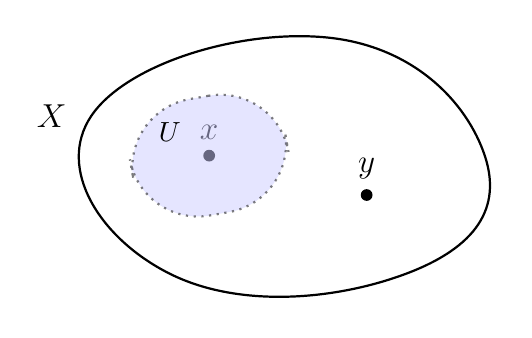
\begin{tikzpicture}[
          point/.style={circle, fill, inner sep=1.5pt},
          set/.style={draw, dotted, thick, rotate=10, minimum width=2cm, minimum height=1.5cm, rounded corners=25pt},
          mylabel/.style={font=\large\itshape}
      ]
        % Draw the topological space X
        \draw[thick] plot [smooth cycle, tension=0.8] coordinates {(0,0) (3,1) (5,-0.5) (4,-2) (1,-2)};
        \node[font=\large] at (-0.5,0) {$X$};
        
        % Draw the points
        \node[point, label={[mylabel]above:$x$}] (x) at (1.5,-0.5) {};
        \node[point, label={[mylabel]above:$y$}] (y) at (3.5,-1) {};
        
        % Draw only one open neighborhood (T0 only requires one direction)
        \node[set, fill=blue!20, opacity=0.5] (Ux) at (x) {};
        
        % Label the neighborhood
        \node[font=\normalsize] at (1,-0.2) {$U$};
      \end{tikzpicture}
      \caption{$t_0$-separability. } 
      \label{fig:t0_separability}
    \end{figure}
  \end{definition}

  \begin{definition}[$t_1$-Separability]
    A topological space $X$ is said to be \textbf{$t_1$-separable} if for each pair of distinct points $x, y \in X$, we can find two neighborhoods $U_x, U_y$ where $y \not\in U_x$ and $x \not\in U_y$. 

    \begin{figure}[H]
      \centering 
      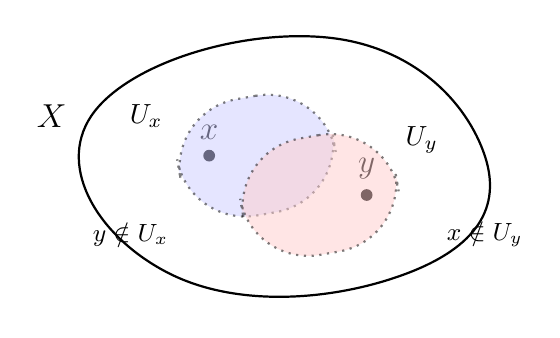
\begin{tikzpicture}[
        point/.style={circle, fill, inner sep=1.5pt},
        set/.style={draw, dotted, thick, rotate=10, minimum width=2cm, minimum height=1.5cm, rounded corners=25pt},
        mylabel/.style={font=\large\itshape}
      ]
        % Draw the topological space X
        \draw[thick] plot [smooth cycle, tension=0.8] coordinates {(0,0) (3,1) (5,-0.5) (4,-2) (1,-2)};
        \node[font=\large] at (-0.5,0) {$X$};
        
        % Draw the points
        \node[point, label={[mylabel]above:$x$}] (x) at (1.5,-0.5) {};
        \node[point, label={[mylabel]above:$y$}] (y) at (3.5,-1) {};
        
        % Draw the open neighborhoods with significant overlap (to show T1 is weaker than Hausdorff)
        \node[set, fill=blue!20, opacity=0.5] (Ux) at ($(x) + (0.6,0)$) {};
        \node[set, fill=red!20, opacity=0.5] (Uy) at ($(y) + (-0.6,0)$) {};
        
        % Label the neighborhoods
        \node[font=\normalsize] at (0.7,0) {$U_x$};
        \node[font=\normalsize] at (4.2,-0.3) {$U_y$};
        
        % Add annotation to clarify that in T1, x ∉ Uy and y ∉ Ux 
        \node[font=\small, align=center] at (0.5,-1.5) {$y \notin U_x$};
        \node[font=\small, align=center] at (5,-1.5) {$x \notin U_y$};
      \end{tikzpicture}
      \caption{$t_1$-separability. } 
      \label{fig:t1_separability}
    \end{figure}
  \end{definition}

  \begin{example}[Nested Interval Topology is Not $t_0$]
    $(0,1)$ with the nested interval topology is not $t_0$-separable, since we can't distinguish $\frac{1}{4}$ and $\frac{1}{3}$.
  \end{example}

  \begin{example}[Cofinite is $t_1$]
    $(0,1)$ with the cofinite topology is $t_0$-separable, since given distinct $x_1, x_2 \in (0,1)$, we can see that $x_1 \in X \setminus {x_2}$ and $x_2 \in X \setminus {x_1}$, which are both elements of the cofinite topology. By existence of these elements, $(0,1)$ is $t_1$-separable. 
  \end{example}

\subsection{Hausdorff Spaces}

  Generally, mathematicians consider the Hausdorff condition as a mild extra conditions on topological spaces that make it much easier to deal with. We will assume that most of the topological spaces we work with are Hausdorff. 

  \begin{definition}[Hausdorff Space]
    A topological space $X$ is called a \textbf{Hausdorff space}, or \textbf{$t_2$-separable}, if for each pair of distinct points $x, y \in X$, there exists neighborhoods $U_x, U_y$ that are disjoint.

    \begin{figure}[H]
      \centering 
      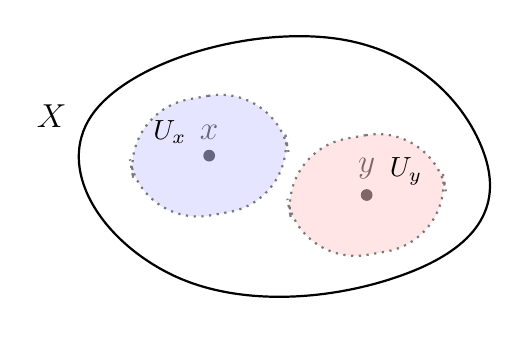
\begin{tikzpicture}[
          point/.style={circle, fill, inner sep=1.5pt},
          set/.style={draw, dotted, thick, rotate=10, minimum width=2cm, minimum height=1.5cm, rounded corners=25pt},
          mylabel/.style={font=\large\itshape}
      ]
        % Draw the topological space X
        \draw[thick] plot [smooth cycle, tension=0.8] coordinates {(0,0) (3,1) (5,-0.5) (4,-2) (1,-2)};
        \node[font=\large] at (-0.5,0) {$X$};

        % Draw the points
        \node[point, label={[mylabel]above:$x$}] (x) at (1.5,-0.5) {};
        \node[point, label={[mylabel]above:$y$}] (y) at (3.5,-1) {};

        % Draw the open neighborhoods
        \node[set, fill=blue!20, opacity=0.5] (Ux) at (x) {};
        \node[set, fill=red!20, opacity=0.5] (Uy) at (y) {};

        % Label the neighborhoods
        \node[font=\normalsize] at (1,-0.2) {$U_x$};
        \node[font=\normalsize] at (4,-0.7) {$U_y$};
      \end{tikzpicture}
      \caption{Every pair of distinct points must satisfy this separability condition in a Hausdorff space.} 
      \label{fig:hausdorff}
    \end{figure}
  \end{definition}

  \begin{theorem}[Limit Points in Hausdorff Spaces]
    Given Hausdorff space $X$ and subset $A \subset X$ a point $x$ is a limit point of $A$ if and only if every neighborhood of $x$ contains infinitely many point of $A$. It immediately follows that every finite point set in a Hausdorff space $X$ is closed. 
  \end{theorem}
  \begin{proof}
    We prove both directions
    \begin{enumerate}
      \item $(\rightarrow)$ Assume that $x$ is a limit point of $A$ with some neighborhood $U_x$ intersecting $A$ in finitely many points. Then, let the points of intersections be 
      \begin{equation}
        \{x_1, ..., x_n\} = A \cap \{U_x \setminus \{x\} \}
      \end{equation}
      But $U_x \setminus \{x\}$ is open $\implies H \equiv \{U_x \setminus ( \{x\} \cup \{x_1, ..., x_n\})\}$ is open. But $H \cap A = \emptyset$, contradicting the assumption that $x$ is a limit point. 

      \item $(\leftarrow)$ Simple. 
    \end{enumerate}
    It suffices to show that every one point set $\{x_0\}$ is closed. If $x$ and $x_0$ are distinct points, then by definition of Hausdorff spaces they have disjoint neighborhoods $U_x$ and $U_{x_0} \implies x \not\in \bar{\{x_0\}} \implies \{x_0\} = \bar{\{x_0\}}$, so $\{x_0\}$ is closed. 
  \end{proof}

  \begin{lemma}[Product of Hausdorff Spaces]
    Arbitrary Cartesian products of Hausdorff spaces is Hausdorff.\footnote{Since this is in the product topology, it immediately follows that the product is also Hausdorff in the finer box topology.}
  \end{lemma}

  \begin{lemma}[Subspaces of Hausdorff Spaces]
    A subspace of a Hausdorff space is Hausdorff. 
  \end{lemma}

  \begin{theorem}[Unique Point of Convergence]
    If a sequence converges in a Hausdorff space $X$, it converges to one point. 
  \end{theorem}
  \begin{proof}
    For if $(x_\alpha)$ converges to $x$ and if $y \neq x$, then we need only choose disjoint neighborhoods of $y$ and $x$ to prove that $(x_\alpha)$, by definition, is not convergent to $y$.
  \end{proof}

  \begin{example}
    The space $(0,1)$ with the nested interval topology is not Hausdorff. In fact, it is impossible to distinguish 2 points $x, y$ if $x, y \in (0, \frac{1}{2})$, meaning that the sequence
    \begin{equation}
        \frac{1}{10}, \frac{2}{10}, \frac{1}{10}, \ldots
    \end{equation}
    converges to both $\frac{1}{10}$ and $\frac{2}{10}$.
  \end{example} 

  \begin{theorem}
    Every metric topology satisfies the Hausdorff Axiom.
  \end{theorem}
  \begin{proof}
    If $x$ and $y$ are distinct points of $(X, d)$, then letting
    \begin{equation}
      \varepsilon = \frac{1}{2} d(x, y)
    \end{equation}
    the triangle inequality implies that $B_\varepsilon (x)$ and $B_\varepsilon (y)$ are disjoint. 
  \end{proof}

\subsection{Regular Spaces}

  \begin{definition}[Regular Spaces]
    Suppose that one-point sets are closed in $X$. Then, $X$ is said to be \textbf{regular}, or \textbf{$t_3$-separable}, if for each pair consisting of a point $x$ and a closed set $C$ disjoint from $x$, there exist disjoint open sets containing $x$ and $C$, respectively. 

    \begin{figure}[H]
      \centering 
      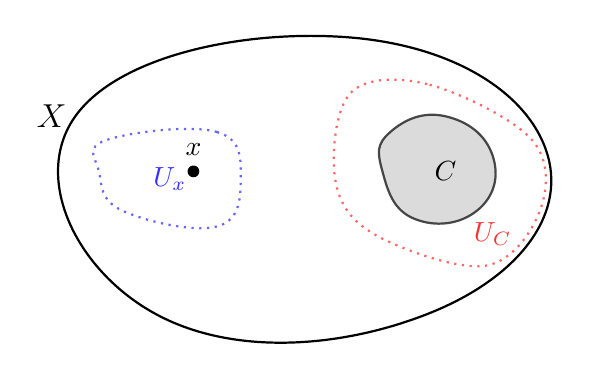
\begin{tikzpicture}[
          point/.style={circle, fill, inner sep=1.5pt},
          closed/.style={draw, thick, fill=gray!40, opacity=0.7},
          open/.style={draw, dotted, thick}
      ]

      % Draw the topological space X
      \draw[thick] plot [smooth cycle, tension=0.8] coordinates {(0,0) (3.5,1) (6,-0.5) (4.5,-2.5) (1,-2.5)};
      \node[font=\large] at (-0.3,0) {$X$};

      % Draw the point x
      \node[point, label={[font=\itshape]above:$x$}] (x) at (1.5,-0.7) {};

      % Draw the closed set C
      \draw[closed] plot [smooth cycle, tension=0.8] coordinates {(4,-0.2) (4.7,0) (5.3,-0.5) (5.1,-1.2) (4.3,-1.3) (3.9,-0.7)};
      \node at (4.7,-0.7) {$C$};

      % Draw the open set containing x
      \draw[open, blue!60, thick] plot [smooth cycle, tension=0.7] coordinates {(0.4,-0.3) (1.8,-0.2) (2.1,-0.8) (1.8,-1.4) (0.6,-1.2) (0.3,-0.7)};
      \node[blue!80] at (1.2,-0.8) {$U_x$};

      % Draw the open set containing C
      \draw[open, red!60, thick] plot [smooth cycle, tension=0.6] coordinates {(3.5,0.3) (4.5,0.4) (5.8,-0.3) (5.9,-1.2) (5.2,-1.9) (3.8,-1.5) (3.3,-0.8)};
      \node[red!80] at (5.3,-1.5) {$U_C$};

      \end{tikzpicture}
      \caption{Regular space.} 
      \label{fig:regular}
    \end{figure}

  \end{definition}

  \begin{lemma}[Product of Regular Spaces]
    Arbitrary Cartesian products of regular spaces is regular. 
  \end{lemma}

  \begin{lemma}[Subspaces of Regular Spaces]
    A subspace of a regular space is regular.  
  \end{lemma}

\subsection{Normal Spaces}

  \begin{definition}[Normal Spaces]
    Suppose that one-point sets are closed in $X$. Then, $X$ is said to be \textbf{normal}, or \textbf{$t_4$-separable}, if for each pair $C, D$ of disjoint closed sets of $X$, there exist disjoint open sets containing $C$ and $D$, respectively. 

    \begin{figure}[H]
      \centering 
      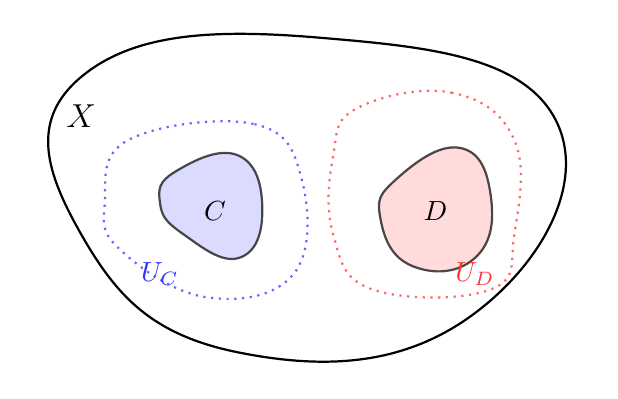
\begin{tikzpicture}[
          closed/.style={draw, thick, fill=gray!40, opacity=0.7},
          open/.style={draw, dotted, thick}
      ]

      % Draw the topological space X
      \draw[thick] plot [smooth cycle, tension=0.8] coordinates {(0,1) (3,1.5) (6,0.5) (5,-2) (2,-2.5) (0,-1)};
      \node[font=\large] at (0,0.5) {$X$};

      % Draw the first closed set C
      \draw[closed, fill=blue!20] plot [smooth cycle, tension=0.8] coordinates {(1.2,-0.2) (2,0) (2.3,-0.7) (2,-1.3) (1.3,-1) (1,-0.6)};
      \node at (1.7,-0.7) {$C$};

      % Draw the second closed set D
      \draw[closed, fill=red!20] plot [smooth cycle, tension=0.8] coordinates {(4,-0.3) (4.8,0.1) (5.2,-0.5) (5,-1.3) (4.2,-1.4) (3.8,-0.8)};
      \node at (4.5,-0.7) {$D$};

      % Draw the open set containing C
      \draw[open, blue!60, thick] plot [smooth cycle, tension=0.7] coordinates {(0.6,0.2) (2.2,0.4) (2.8,-0.3) (2.7,-1.5) (1.6,-1.8) (0.5,-1.2) (0.3,-0.6)};
      \node[blue!80] at (1,-1.5) {$U_C$};

      % Draw the open set containing D
      \draw[open, red!60, thick] plot [smooth cycle, tension=0.7] coordinates {(3.5,0.6) (4.7,0.8) (5.5,0.2) (5.5,-1) (5.2,-1.7) (3.7,-1.7) (3.2,-1) (3.2,0)};
      \node[red!80] at (5,-1.5) {$U_D$};

      \end{tikzpicture}
      \caption{Normal space.} 
      \label{fig:normal}
    \end{figure}
  \end{definition}

  However, neither products nor subspaces of normal spaces are necessarily normal. 
  a subspace of a normal space is not necessarily normal; a product of normal spaces is not necessarily normal. 

  \begin{theorem}
    Every metrizable space is normal. 
  \end{theorem}

  \begin{theorem}
    Every compact Hausdorff space is normal. 
  \end{theorem}

  \begin{theorem}
    Every regular space with a countable basis is normal. 
  \end{theorem}

  \begin{theorem}
    Every well-ordered set $X$ is normal in the order topology. 
  \end{theorem}

\subsection{The Urysohn Lemma}

  \begin{theorem}[Urysohn Lemma]
    Let $X$ be a normal space, and let $A, B$ be disjoint closed subsets of $X$. Let $[a,b]$ be a closed interval in the real line. Then there exists a continuous map
    \begin{equation}
      f: X \longrightarrow [a,b]
    \end{equation}
    such that $f(x) = a$ for every $x \in A$ and $f(x) = b$ for every $x \in B$. 
  \end{theorem}

  \begin{definition}[Separation by Continuous Function]
    If $A$ and $B$ are two subsets of the topological space $X$, and if there is a continuous function $f: X \longrightarrow [0,1]$ such that $f(A) = \{0\}$ and $f(B) = \{1\}$, it is said that \textbf{$A$ and $B$ can be separated by a continuous function}. 
  \end{definition}

  More colloquially, the lemma states that if every pair of disjoint closed sets in $X$ can be separated by disjoint open sets, then each such pair can be separated by a continuous function. 

  \begin{theorem}[Tietze Extension Theorem]
    Let $X$ be a normal space and let $A$ be a closed subset of $X$. 
    \begin{enumerate}
      \item Any continuous map of $A$ into the closed interval $[a,b] \subset \mathbb{R}$ may be extended to a continuous map of all $X$ into $[a,b]$. 
      \item Any continuous map $A$ into the reals $\mathbb{R}$ may be extended to a continuous map of all of $X$ into $\mathbb{R}$. 
    \end{enumerate}
  \end{theorem}

\subsection{The Urysohn Metrization Theorem}

  \begin{theorem}[Urysohn Metrization Theorem]
    Every regular space $X$ with a countable basis is metrizable. 
  \end{theorem}

  \begin{theorem}[Imbedding Theorem]
    Let $X$ be Hausdorff. Suppose that 
    \begin{equation}
      \{f_\alpha\}_{\alpha \in J}, \; f_\alpha: X \longrightarrow \mathbb{R}
    \end{equation}
    is a collection of continuous functions satisfying the requirement that for each point $x_0 \in X$ and each neighborhood $U$ of $x_0$, there is an index $\alpha$ such that $f_\alpha$ is positive at $x_0$ and vanishes outside $U$. Then, the function 
    \begin{equation}
      F: X \longrightarrow \mathbb{R}^J, \; F(x) \equiv \big( f_\alpha (x)\big)_{\alpha \in J}
    \end{equation}
    is an \textbf{imbedding} of $X$ in $\mathbb{R}^J$.
  \end{theorem}


\section{Homotopies}  

\subsection{Homotopy and Path Homotopy}

  The concept of homotopies is dealt with in algebraic topology, but it is worthwhile to mention it now. 

  \begin{definition}[Homotopy]
    Two continuous paths from $x$ to $y$ in topological space $X$ is \textbf{homotopic} if one can be continuously "deformed" into the other, such a deformation being the \textbf{homotopy} between two functions. The set of linearly homotopic paths form a relation, and thus \textbf{homotopy classes} can be further defined. 
    \begin{figure}[H]
      \centering 
      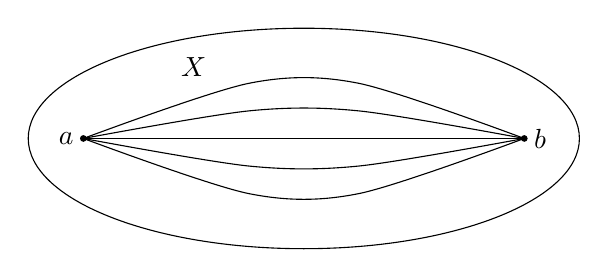
\begin{tikzpicture}[scale=0.7]
        \draw (0,0) ellipse (5 and 2);
        \draw[fill] (-4,0) circle (0.05);
        \draw[fill] (4,0) circle (0.05);
        \draw plot [smooth] coordinates {(-4,0) (-1,1) (1,1) (4,0)};
        \draw (-4,0)--(4,0);
        \draw plot [smooth] coordinates {(-4,0) (-1,0.5) (1,0.5) (4,0)};
        \draw plot [smooth] coordinates {(-4,0) (-1,-0.5) (1,-0.5) (4,0)};
        \draw plot [smooth] coordinates {(-4,0) (-1,-1) (1,-1) (4,0)};
        \node at (-2,1.3) {$X$};
        \node[left] at (-4,0) {$a$};
        \node[right] at (4,0) {$b$};
      \end{tikzpicture}
      \caption{Visually, the set of all the curves in the space $X$ as shown are in a single homotopy class.} 
      \label{fig:single_homotopy_class}
    \end{figure}
  \end{definition}

  It is clear that the space $X$ consists of a single homotopy class of curves from $a$ to $b$. However, a space may have an infinite number of such classes. 

  \begin{figure}[H]
    \centering 
    \begin{tikzpicture}[scale=0.7]
      \draw (0,0) ellipse (5 and 2);
      \draw[fill] (-4,0) circle (0.05);
      \draw[fill] (4,0) circle (0.05);
      \draw plot [smooth] coordinates {(-4,0) (-1,1) (1,1) (4,0)};
      \node[left] at (-4,0) {$a$};
      \node[right] at (4,0) {$b$};
      \draw (0,0) circle (1);
      \node at (-2,1.3) {$Y$};
      \draw[blue] plot [smooth] coordinates {(-4,0) (-2,0.5) (-1,1) (1,1) (1,-1) (-1,-1) (-1,1) (1,1) (2,0.5) (4,0)};
    \end{tikzpicture}
    \caption{Let us define the space $Y \equiv X \setminus C$ where $C$ is a circular region in $X$. Then, $Y$ has an infinite number of homotopy classes. We show two curves, that are in two different homotopy classes. }
    \label{fig:homotopy_class}
  \end{figure}

  \begin{definition}[Simply Connected Set]
    A \textbf{simply connected set} is a set such that all paths between any two given points are homotopic. That is, a simply connected set has one homotopy class. 
  \end{definition}

\subsection{The Fundamental Group}


\section{Exercises} 

\subsection{Group Like Structures}

  \begin{exercise}[Math 401 Spring 2025 Midterm 2]
    Listed. 
    \begin{enumerate}
      \item Let $G$ be a finite group with an even number of elements. Show that $G$ contains an element of order $2$. 
      \item Prove that a group of order $10$ contains an element of order $5$. 
    \end{enumerate}
  \end{exercise}
  \begin{solution}
    Listed. 
    \begin{enumerate}
      \item We know that $e^{-1} = e$, and so remove it from $G$. Then $G$ has an odd number of elements. Now as long as $G$ is nonempty, we can remove $a, a^{-1}$, resulting in an odd cardinality. Since $G$ is finite, this must terminate, and so there must be a case where $a = a^{-1} \implies \ord(a) = 2$. 
      \item Assume that there is no element of order $5$. Then from above it must contain an element of order $2$, and let us call it $a \in G$. $\ord(e) = 1$ obviously. If any $b \in G$ had order 10, then $G = Z_{10}$, which would mean that $\ord(b^5) = 2$. Therefore every element other than the identity must have order $2$. But then given $a, b, ab \in G$, $ab \neq a, b$ since $ab = a \implies b = e$, and this is precisely the Klein 4 group. This subgroup has an order that doesn't divide 10, contradicting Lagrange's theorem. 
    \end{enumerate}
  \end{solution}

  \begin{exercise}[Shifrin 6.1.1]
    Which of the following are groups?
    \begin{enumerate}
      \item[(a)] $\{1,3,7,9\} \subset \mathbb{Z}_{10}$, with operation multiplication
      \item[(b)] $\{0,2,4,6\} \subset \mathbb{Z}_{10}$, with operation addition
      \item[(c)] $\{x \in \mathbb{Q} : 0 < x \leq 1\}$, with operation multiplication
      \item[(d)] the set of all positive irrational real numbers, with operation multiplication
      \item[(e)] the set of imaginary numbers $ix, x \in \mathbb{R}$, with operation addition
      \item[(f)] the set of complex numbers of modulus 1, with operation multiplication
      \item[(g)] $\mathbb{Z}$ with operation $a \bullet b = a + b + 1$
      \item[(h)] $\mathbb{Z}$ with operation $a \bullet b = a - b$
      \item[(i)] $\mathbb{Q} - \{1\}$ with operation $a \bullet b = a + b - ab$
    \end{enumerate}
  \end{exercise}
  \begin{solution}
    Listed. We will denote the sets in question to be $G$. 
    \begin{enumerate}
      \item[(a)] Is a group since product of 2 odds is odd, so is closed. Also we have $1$ as the identity with $3^{-1} = 7, 7^{-1} = 3, 9^{-1} = 9$. It is associative since multiplication on $\mathbb{Z}_{10}$ is associative. 
      \item[(b)] Not a group since $4 + 4 = 8 \not\in G$. 
      \item[(c)] Not a group since $1/2 \in G$ but $(1/2)^{-1} = 2 \not\in G$. 
      \item[(d)] Not a group since $\sqrt{2} \times \sqrt{2} 2  \not\in G$. 
      \item[(e)] Is a group since identity is $0 = 0i$, $ix + iy = i (x + y)$ with $x + y \in \mathbb{R}$, and $-(ix) = i (-x)$ where $-x \in \mathbb{R}$. 
      \item[(f)] Is a group since this is a representation of $O(2)$. 
      \item[(g)] Is a group since this is obviously closed under $\mathbb{Z}$ since $+_{\mathbb{Z}}$ is closed. Now assume that $i$ is the identity. Then $a \bullet i = a + i + 1 = a \implies i = -1$. Therefore $a \bullet a^{-1} = a + a^{-1} + 1 = -1 \implies a^{-1} = -a - 2$. This is associative since 
      \begin{equation}
        (a \bullet b) \bullet c = (a + b + 1) \bullet c = a + b + c + 2 = a \bullet (b + c + 1) = a \bullet (b \bullet c)
      \end{equation}
      \item[(h)] Not a group since it is not associative. Note $(a \bullet b) \bullet c = (a - b) \bullet c = a - b - c$, while $a \bullet (b \bullet c) = a \bullet (b - c) = a - b + c$. 
      \item[(i)] Is a group. We claim that it is closed. Assume not; given $a, b \neq 1$, 
        \begin{equation}
          a \bullet b = a + b - ab = 1 \implies 0 = ab - a - b + 1 = (a - 1)(b-1) 
        \end{equation}
        which means $a = 1$ or $b = 1$, which is a contradiction. As for the identity, $a \bullet i = a + i - ai = a \implies 0 = i - ai = i (1 - a) \implies i = 0$ since $a \neq 1$. We can define the inverse by solving 
        \begin{equation}
          0 = a \bullet a^{-1} = a + a^{-1} - a a^{-1} \implies a^{-1} (1 - a) = -a \implies a^{-1} = \frac{a}{a-1}
        \end{equation}
        which is well-defined since $a \neq 1$. Finally, it is associative since 
        \begin{align}
          (a \bullet b) \bullet c & = (a + b - ab) \bullet c \\
                                  & = a + b - ab + c - ac - bc - abc \\
                                  & = a + b + c - bc - ab - ac - abc \\
                                  & = a \bullet (b + c - bc) \\
                                  & = a \bullet (b \bullet c)
        \end{align}
    \end{enumerate}
  \end{solution}

  \begin{exercise}[Shifrin 6.1.10]
    \begin{enumerate}
      \item[(a)] Let $G$ be a group. Prove that $(ab)^2 = a^2b^2$ for all $a,b \in G$ if and only if $G$ is abelian.
      \item[(b)] Prove that if every element (other than the identity element) of a group $G$ has order 2, then $G$ is abelian.
    \end{enumerate}
  \end{exercise}
  \begin{solution}
    For (a), if $G$ is abelian, then 
    \begin{equation}
      (ab)^2 = (ab) (ab) = a (ba) b = a (ab) b = (aa) (bb) = a^2 b^2
    \end{equation}
    If the identity holds, then 
    \begin{equation}
      (ab)^2 = a^2 b^2 \implies (a^{-1} a) (ba) (b b^{-1}) = a^{-1} (ab)(ab) b^{-1} = a^{-1} a^2 b^2 b^{-1} \implies ba = ab
    \end{equation} 
    For (b), since we have $a^2 = e, b^2 = e$, and $(ab)^2 = e$, from (a) $G$ is abelian. 
  \end{solution}

  \begin{exercise}[Shifrin 6.1.17]
    \begin{enumerate}
      \item[(a)] A group has four elements $a$, $b$, $c$, and $d$, subject to the rules $ca = a$ and $d^2 = a$. Fill in the entire multiplication table at the left below.
      
      \begin{tabular}{c|cccc}
        $\cdot$ & $a$ & $b$ & $c$ & $d$ \\
        \hline
        $a$ & & & & \\
        $b$ & & & & \\
        $c$ & $a$ & & & \\
        $d$ & & & & $a$ \\
      \end{tabular}
      
      \item[(b)] A group has six elements $a$, $b$, $c$, $d$, $e$, and $f$, subject to the rules $ae = a$, $bd = a$, $c^2 = a$, and $df = a$. Fill in the entire multiplication table at the right above.
      
      \begin{tabular}{c|cccccc}
        $\cdot$ & $a$ & $b$ & $c$ & $d$ & $e$ & $f$ \\
        \hline
        $a$ & & & & & $a$ & \\
        $b$ & & & & $a$ & & \\
        $c$ & & & $a$ & & & \\
        $d$ & & & & & & $a$ \\
        $e$ & & & & & & \\
        $f$ & & & & & & \\
      \end{tabular}
    \end{enumerate}
  \end{exercise}
  \begin{solution}
    We can see that $ca = a \implies c = ca a^{-1} = a a^{-1} = i$, so $c$ is the identity. We can fill in the row and column of $c$. Then, we can figure out what $bd$ is. It cannot be $b$ or $d$ since $c$ is the unique identity, so it must be either $a$ or $c$. It cannot be $a$ since then $bd = a = d^2$, and so $b = d$. So it must be $c$. By the same logic we can fill out the rest of the rows and columns. 

    \begin{tabular}{c|cccc}
      $\cdot$ & $a$ & $b$ & $c$ & $d$ \\
      \hline
      $a$ & $c$ & $d$ & $a$ & $b$ \\
      $b$ & $d$ & $a$ & $b$ & $c$ \\
      $c$ & $a$ & $b$ & $c$ & $d$ \\
      $d$ & $b$ & $c$ & $d$ & $a$ \\
    \end{tabular}

    By the same logic as the previous, we can immediately see that $ae = a \implies e$ is the identity. The formal logic above can be simplified down to saying that there can be no two of the same elements in the same row or column, since if it were, then we are saying that $xy = xz \implies y = z$, which cannot be the case since $y$ and $z$ are distinct. So $fb = a$. We can also deduce that $da = ab$ and $ba = af$. At this point, we can recognize that this is the Dihedral group of order $6$, and so we fill in the rest of the multiplication table. 

    \begin{tabular}{c|cccccc}
      $\cdot$ & $a$ & $b$ & $c$ & $d$ & $e$ & $f$ \\
      \hline
      $a$ & c & f & e & b & a & d \\
      $b$ & d & e & f & a & b & c \\
      $c$ & e & d & a & f & c & b \\
      $d$ & f & c & b & e & d & a \\
      $e$ & a & b & c & d & e & f \\
      $f$ & b & a & d & c & f & e
    \end{tabular}
  \end{solution}

\subsection{Subgroups and Quotient Groups}

  \begin{exercise}[Shifrin 6.2.2]
    Prove that $\mathbb{Z}_7^{\times} \cong \mathbb{Z}_6$. (It is crucial to remember that we multiply in $\mathbb{Z}_7^{\times}$ and add in $\mathbb{Z}_6$.)
  \end{exercise}
  \begin{solution}
    Both groups are of order 6, and so $\mathbb{Z}_7^\times$---which is indeed a group (since it is the group of units of the ring $(\mathbb{Z}_7, +, \times)$)---must be isomorphic to either $\mathbb{Z}_6$ or $S_3$. However, $S_3$ is not abelian, while $\mathbb{Z}^\times_7$ is, so it must be the case that it is isomorphic to $\mathbb{Z}_6$. 
  \end{solution}

  \begin{exercise}[Shifrin 6.2.15.a/b]
    The \textbf{dihedral group} of order $2n$, denoted $\mathcal{D}_n$, is given by $\{\rho^i\psi^j : 0 \leq i < n, 0 \leq j \leq 1\}$ subject to the rules $\rho^n = e$, $\psi^2 = e$, and $\psi\rho\psi^{-1} = \rho^{-1}$.
    \begin{enumerate}
      \item Check this is really a group. That is, what is $(\rho^i\psi^j)^{-1}$, and what is the product $(\rho^i\psi^j)(\rho^k\psi^\ell)$?
      \item Check that $\mathcal{T} \cong \mathcal{D}_3$ and $S_q \cong \mathcal{D}_4$.
    \end{enumerate}
  \end{exercise}
  \begin{solution}
    We check the properties of a group. The following identity is useful: 
    \begin{equation}
      (\psi \rho \psi^{-1})^{n-i} = (\rho^{-1})^{n-i} \implies \psi \rho^{n-i} \psi^{-1} = \rho^i \implies \psi \rho^{n-i} = \rho^i \psi
    \end{equation}
    \begin{enumerate}
      \item \textit{Closure}. From simplifying according to the first two rules, we will automatically adjust the exponents to be $i, k < n$ (by subtracting out multiples of $n$) and $j \in \{0, 1\}$ (by subtracting out multiples of $2$). Going case by case, 
      \begin{enumerate}
        \item $j = 0, l = 0$. $\rho^i \rho^k = \rho^{i+k}$. 
        \item $j = 0, l = 1$. $\rho^i \rho^k \psi = \rho^{i+k} \psi$. 
        \item $j = 1, l = 0$. $\rho^i \psi \rho^k = \rho^i \rho^{n-k} \psi = \rho^{n-k+i} \psi$. 
        \item $j = 1, l = 1$. $\rho^i \psi \rho^k \psi = \rho^i \psi \psi \rho^{n-k} = \rho^i \rho^{n-k} = \rho^{n-k+i}$. 
      \end{enumerate}
      \item \textit{Identity}. The identity is $e = \rho^0 \psi^0$. We can see that $e \rho^i \psi^j = \rho^i \psi^j e = \rho^{i+0} \psi^j$. 
      \item \textit{Inverse}. We have $\psi \rho \psi^{-1} = \psi \rho \psi = \rho^{-1} \implies \psi \rho = \rho^{-1} \psi^{-1} = (\psi \rho)^{-1}$. Therefore, 
      \begin{equation}
        (\rho^i \psi^j)^{-1} = \begin{cases} 
          \rho^{n - i} & \text{ if } j = 0  \\
          \rho^{i} \psi & \text{ if } j = 1
        \end{cases}
      \end{equation}
      which are both of the correct form and therefore in $\mathcal{D}_n$. To verify, we see that $\rho^i \rho^{n-i} = \rho^n = e$, and $(\rho^i \psi) (\rho^i \psi) = \rho^i \psi \psi \rho^{n-i} = \rho^i \rho^{n-i} = e$.  
      \item \textit{Associativity}. Can also be proven tediously but problem only asked to state the product and inverse.  
    \end{enumerate} 

    For (b) for $\mathcal{T}$, we can explicitly look at the multiplication tables and see that they are isomorphic. We denote $r_1, r_2$ as the 120 and 240 degree rotations, and $f_1, f_2, f_3$ as the flips across each axis. 

    \begin{figure}[H]
      \centering
      \begin{subfigure}[b]{0.48\textwidth}
        \centering
        \begin{tabular}{c|cccccc}
          & $e$ & $\rho$ & $\rho^2$ & $\psi$ & $\rho\psi$ & $\rho^2\psi$ \\
          \hline
          $e$ & $e$ & $\rho$ & $\rho^2$ & $\psi$ & $\rho\psi$ & $\rho^2\psi$ \\
          $\rho$ & $\rho$ & $\rho^2$ & $e$ & $\rho^2\psi$ & $\psi$ & $\rho\psi$ \\
          $\rho^2$ & $\rho^2$ & $e$ & $\rho$ & $\rho\psi$ & $\rho^2\psi$ & $\psi$ \\
          $\psi$ & $\psi$ & $\rho^2\psi$ & $\rho\psi$ & $e$ & $\rho^2$ & $\rho$ \\
          $\rho\psi$ & $\rho\psi$ & $\psi$ & $\rho^2\psi$ & $\rho$ & $e$ & $\rho^2$ \\
          $\rho^2\psi$ & $\rho^2\psi$ & $\rho\psi$ & $\psi$ & $\rho^2$ & $\rho$ & $e$
        \end{tabular}
        \caption{$\mathcal{D}_3$}
      \end{subfigure}
      \hfill 
      \begin{subfigure}[b]{0.48\textwidth}
        \centering
        \begin{tabular}{c|cccccc}
          & $e$ & $r_1$ & $r_2$ & $f_1$ & $f_2$ & $f_3$ \\
          \hline
          $e$ & $e$ & $r_1$ & $r_2$ & $f_1$ & $f_2$ & $f_3$ \\
          $r_1$ & $r_1$ & $r_2$ & $e$ & $f_3$ & $f_1$ & $f_2$ \\
          $r_2$ & $r_2$ & $e$ & $r_1$ & $f_2$ & $f_3$ & $f_1$ \\
          $f_1$ & $f_1$ & $f_2$ & $f_3$ & $e$ & $r_2$ & $r_1$ \\
          $f_2$ & $f_2$ & $f_3$ & $f_1$ & $r_1$ & $e$ & $r_2$ \\
          $f_3$ & $f_3$ & $f_1$ & $f_2$ & $r_2$ & $r_1$ & $e$
        \end{tabular}
        \caption{$\mathcal{T}$}
      \end{subfigure}
    \end{figure}

    For $S_q$, it is tedious to write the full table, so we construct the isormorphisms using the generators. For $S_q$, the symmetry group of the square consists of 8 elements: the 4 rotations $r_1, r_2, r_3, r_4$ (of 90, 180, 270, and 360=0 degrees), and the flips $f_1, f_2, f_3, f_4$ (across each axis). Now we construct the function $g: \mathcal{D}_3 \rightarrow \mathcal{T}$ such that $f(\rho) = r_1$ and $f(\psi) = f_1$. Then we can see that 
    \begin{equation}
      g(\rho^4) = g(e) = e = r_1^4 = g(\rho^4), \qquad g(\psi^2) = g(e) = e = f_1^2 = g(\psi)^2
    \end{equation}
    since 90 degrees rotated 4 times is $0$ degrees, the identity, and two flips across the same axis is also the identity. Finally, we have 
    \begin{equation}
      g(\psi \rho \psi) = g(\rho^{-1}) = r_1^{-1} = r_3 = f_1 r_1 f_1 = g(\psi) g(\rho) g(\psi)
    \end{equation}
    Where $r_1^{-1} = r_3$ since a rotation of 270 after a 90 is the same as rotation by 360=0, and $r_3 = f_1 r_1 f_1$ is the change of basis symmetry observed in Shifrin Example 6.1.5. Therefore the rules match, making it a homomorphism, and since the order is the same ($\mathcal{D}_3$ has $4 \times 2 = 8$ elements from looking at the indices), this is an isomorphism. 
  \end{solution}

  \begin{exercise}[Shifrin 6.3.8]
    Let $H \subset G$ be a subgroup, and let $a \in G$ be given. Prove that $aHa^{-1} \subset G$ is a subgroup (called a \textbf{conjugate subgroup} of $H$). Prove, moreover, that it is isomorphic to $H$ (cf. Exercise 6.2.12).
  \end{exercise}
  \begin{solution}
    Let $x, y \in aHa^{-1}$. Then $x = a h_x a^{-1}, y = a h_y a^{-1}$ for some $h_x, h_y \in H$. Therefore, 
    \begin{enumerate}
      \item It is closed. $xy = (a h_x a^{-1}) (a h_y a^{-1}) = a h_x (a^{-1} a) h_y a^{-1} = a h_x h_y a^{-1} \in aHa^{-1}$ since $h_x h_y \in H$ by closure. 
      \item It has an identity since $e \in H \implies a e a^{-1} = a a^{-1} = e \in aHa^{-1}$. 
      \item It has inverses since given $x \in H$ as above with inverses $x^{-1}$, we see that $(a x a^{-1})^{-1} = (a^{-1})^{-1} x^{-1} a^{-1} = a x^{-1} a^{-1} \in a H a^{-1}$ since $x^{-1} \in H$ by $H$ being a group. 
      \item Associativity is inherited from $G$. 
    \end{enumerate} 
    It suffices to show that this is injective, since the map $\iota : H \rightarrow a H a^{-1}$ is surjective by definition. Given $x, y \in a H a^{-1}$ with $x = y$, we have $a h_x a^{-1} = a h_y a^{-1}$, and multiplying by $a$ on the right and then $a^{-1}$ on the left, we get $h_x = h_y$.
  \end{solution}

  \begin{exercise}[Shifrin 6.3.11]
    Prove that a group of order $n$ has a proper subgroup if and only if $n$ is composite.
  \end{exercise}
  \begin{solution}
    We prove bidirectionally. Call the group $G$ and subgroup $H$. 
    \begin{enumerate}
      \item $(\rightarrow)$. Assume $n$ is prime. Then by Lagrange's theorem $|H|$ must divide $n$, and so $|H| = 1$ or $n$, neither of which results in a proper subgroup. 
      \item $(\leftarrow)$. Assume $G$ has a proper subgroup $H$. Since it is proper, $|H| \neq 1, n$. Then by Lagrange's theorem, $|H|$ divides $n$, which implies that $n$ is composite. 
    \end{enumerate}
  \end{solution}

  \begin{exercise}[Shifrin 6.3.13]
    Suppose $H, K \subset G$ are subgroups of orders $5$ and $8$, respectively. Prove that $H \cap K = \{e\}$.
  \end{exercise}
  \begin{solution}
    Let us take an arbitrary element in $x \in H \cap K$ and consider the cyclic group $\langle x \rangle$. By Lagrange's Theorem, the order $|x|$ in $H$ must be either $1$ or $5$, while the order in $K$ must be $1, 2, 4, 8$. Therefore, $|x| = 1$ and so $x = e$. 
  \end{solution}

  \begin{exercise}[Shifrin 6.3.17]
    \begin{enumerate}
      \item Prove that a group $G$ of even order has an element of order $2$. (Hint: If $a \neq e$, $a$ has order $2$ if and only if $a = a^{-1}$.)
      \item Suppose $m$ is odd, $|G| = 2m$, and $G$ is abelian. Prove $G$ has precisely one element of order $2$. (Hint: If there were two, they would provide a Klein four-group.)
      \item Prove that if $G$ has exactly one element of order $2$, then it must be in the center of $G$.
    \end{enumerate}
  \end{exercise}
  \begin{solution}
    Listed. 
    \begin{enumerate}
      \item Assume the contrary and take $H = G \setminus \{e\}$. Then $|H|$ is odd, and since no element has order $2$, every element must be associated with a unique inverse $a, a^{-1}$. But this cannot happen since $|H|$ is odd. Therefore there must be at least one element of order $2$. 

      \item It has at least 1 element of order 2 from (1). Now assume that there are two, call them $a, b$. Then $ab \neq a, b$ and $ab$ also has order $2$ since $(ab)(ab) = abba = aa = e$. Therefore, calling $c = ab$, we have $ac = ca = aab = b$ and $bc = cb = abb = a$. This fully defines the multiplication table for the Klein 4 group $K$ of order $4$. Therefore, by Lagrange's theorem, we have found a subgroup $K$ and so $|K|$ must divide $G$. However, this would mean that $m$ must be even, a contradiction. Therefore there is only one such unique $a$. 

      \item Given $a \in G$ with $|a| = 2$, we wish to show that it is an element of $Z = \{ b \in G \mid bx = xb \forall x \in G\}$.\footnote{I am using the definition of center defined in Shifrin 6.3.7.} Consider $z = x^{-1} a x$. We have 
      \begin{equation}
        z^2 = (x^{-1} a x)^2 = x^{-1} a x x^{-1} a x = x^{-1} a^2 x = x^{-1} x = e
      \end{equation}
      which means that $z$ also has order $2$. But since this is unique, it must be that $z = a$. Therefore, by multiplying $x$ on the left, we get 
      \begin{equation}
        x^{-1} a x = a \implies ax = xa
      \end{equation}
    \end{enumerate}
  \end{solution}
  
  \begin{exercise}[Assigned]
    Find all group homomorphisms $\mathbb{Z}_n \to \mathbb{Z}_m$. (Your answer will depend on $n$ and $m$.) 
  \end{exercise}
  \begin{solution}
    Given a homomorphism, $f$, we must have $f(0) = 0$. Let $f(1) = k$. Note that the value of $f(1) = k$ completely determines the homomorphism since the image of every other $l \in \mathbb{Z}_n$ is defined by 
    \begin{equation}
      f(l) = f(\underbrace{1 + \ldots + 1}_{l \text{ times}}) = \underbrace{k + \ldots + k}_{l \text{ times}}
    \end{equation}
    Since the image of $f$ must be a cyclic subgroup of $\mathbb{Z}_m$, we must satisfy 
    \begin{align}
      0 = f(0) & = f(\underbrace{1 + \ldots + 1}_{n \text{ times}}) \\
               & = \underbrace{k + \ldots + k}_{n \text{ times}} 
    \end{align}
    and so $m \mid nk$. Therefore, $k$ must be a multiple of $m/\gcd(n, m)$. So all homomorphisms are determined by the set 
    \begin{equation}
      \bigg\{ k = \frac{a m}{\gcd(n, m)} \; \bigg| \; a \in \mathbb{N}, 0 \leq k \leq m-1 \bigg\}
    \end{equation}
    which we can see ranges from $0 \leq a < \gcd(n, m)$, and so the total number of homomorphisms is $\gcd(n, m)$. Note that there is always the trivial homomorphism when $a = 0$, i.e. everything maps to $0$. For example, if we have $f: \mathbb{Z}_{14} \to \mathbb{Z}_{21}$, we have $k = 0, 3, 6, 9, 12, 15, 18$. 
  \end{solution}

\subsection{Group Actions}

\subsection{Product Groups}

\subsection{Ring Like Structures}

  \begin{exercise}[Shifrin 1.2.1]
    For each of the following pairs of numbers $a$ and $b$, find $d = \gcd(a,b)$ and express $d$ in the form $ma+nb$ for suitable integers $m$ and $n$.
    \begin{enumerate}
      \item[(a)] $14, 35$
      \item[(b)] $56, 77$
      \item[(c)] $618, 336$
      \item[(d)] $2873, 6643$
      \item[(e)] $512, 360$
      \item[(f)] $4432, 1080$
    \end{enumerate}
  \end{exercise}
  \begin{solution}
    Listed. 
    \begin{enumerate}
      \item $d = 7 = (-2) \cdot 14 + (1) \cdot 35$. 
      \item $d = 7 = (-4) \cdot 56 + 3 \cdot 77$. 
      \item $d = 6 = -25 \cdot 618 + 46 \cdot 336$ 
      \item $d = 13 = 37 \cdot 2873 + (-16) \cdot 6643$. 
      \item $d = 8 = 19 \cdot 512 + (-27) \cdot 360$. 
      \item $d = 8 = 29 \cdot 4432 + (-119) \cdot 1080$. 
    \end{enumerate}
  \end{solution}

  \begin{exercise}[Shifrin 1.2.2]
    You have at your disposal arbitrarily many 4-cent stamps and 7-cent stamps. What are the postages you can pay? Show in particular that you can pay all postages greater than 17 cents.
  \end{exercise}

  \begin{exercise}[Shifrin 1.2.3]
    Prove that whenever $m \neq 0$, $\gcd(0, m) = |m|$.
  \end{exercise}

  \begin{exercise}[Shifrin 1.2.4]
    \begin{enumerate}
      \item[(a)] Prove that if $a|x$ and $b|y$, then $ab|xy$.
      \item[(b)] Prove that if $d = \gcd(a, b)$, then $\gcd(\frac{a}{d}, \frac{b}{d}) = 1$.
    \end{enumerate}
  \end{exercise}

  \begin{exercise}[Shifrin 1.2.5]
    Prove or give a counterexample: the integers $q$ and $r$ guaranteed by the division algorithm, Theorem 2.2, are unique.
  \end{exercise}

  \begin{exercise}[Shifrin 1.2.6]
     Prove or give a counterexample. Let $a, b \in \mathbb{Z}$. If there are integers $m$ and $n$ so that $d = am + bn$, then $d = \gcd(a, b)$.
  \end{exercise}

  \begin{exercise}[Shifrin 1.2.7]
    Generalize Proposition 2.5: if $\gcd(m, c) = 1$ and $m|cz$, then prove $m|z$.
  \end{exercise}
  \begin{solution}
    Let $\mathrm{gcd}(m, c) = 1$ and $m | cz$. Then there exists $a, b \in \mathbb{Z}$ such that $am + bc = 1$. Multiply both sides of the equation by $z$ to get by the distributive property 
    \begin{equation}
      (am + bc) z = amz + bcz = z
    \end{equation} 
    $m | amz$ and $m | cz \implies m | bcz$. Therefore, the sum of the two, which is equal to $z$, must be divisible by $m$. Therefore $m | z$. 
  \end{solution}

  \begin{exercise}[Shifrin 1.2.8]
    Suppose $a, b, n \in \mathbb{N}$, $\gcd(a, n) = 1$, and $\gcd(b, n) = 1$. Prove or give a counterexample: $\gcd(ab, n) = 1$.
  \end{exercise}

  \begin{exercise}[Shifrin 1.2.9]
    Prove that if $p$ is prime and $p|(a_1 a_2 \ldots a_n)$, then $p|a_j$ for some $j$, $1 \leq j \leq n$. (Hint: Use Proposition 2.5 and induction.)
  \end{exercise}

  \begin{exercise}[Shifrin 1.2.10]
    Given a positive integer $n$, find $n$ consecutive composite numbers.
  \end{exercise}

  \begin{exercise}[Shifrin 1.2.11]
    Prove that there are no integers $m, n$ so that $(\frac{m}{n})^2 = 2$. (Hint: You may start by assuming $m$ and $n$ are relatively prime. Why? Then use Exercise 1.1.3.)
  \end{exercise}

  \begin{exercise}[Shifrin 1.2.12]
    Find all rectangles whose sides have integral lengths and whose area and perimeter are equal.
  \end{exercise}

  \begin{exercise}[Shifrin 1.2.13]
    Given two nonzero integers $a, b$, in analogy with the definition of $\gcd(a, b)$, we define the \textbf{least common multiple} $\operatorname{lcm}(a, b)$ to be the positive number $\mu$ with the properties:
    \begin{enumerate}
      \item[(i)] $a|\mu$ and $b|\mu$, and
      \item[(ii)] if $s \in \mathbb{Z}$, $a|s$ and $b|s \Rightarrow \mu|s$.
    \end{enumerate}
    Prove that
    \begin{enumerate}
      \item[(a)] if $\gcd(a, b) = 1$, then $\mu = ab$. (Hint: If $\gcd(a, b) = 1$, then there are integers $m$ and $n$ so that $1 = ma + nb$; therefore, $s = mas + nbs$.)
      \item[(b)] more generally, if $\gcd(a, b) = d$, then $\mu = ab/d$.
    \end{enumerate}
  \end{exercise}
  \begin{solution}
    Listed. 
    \begin{enumerate}
      \item We can simply verify the two properties. Since $\mu = ab$, $a | \mu$ and $b | \mu$ trivially by the existence of $b$ and $a$, respectively. As for the second property, let $s \in \mathbb{Z}$ exist such that $a | s$ and $b | s$. Since $a | s$, $s = xa$ for some $x \in \mathbb{Z}$. But since $b | s$, $b | xa$. Since $\mathrm{gcd}(a, b) = 1$ by assumption, the result in [Shifrin 1.2.7] tells us that $b | x$, i.e. there exists some $k \in \mathbb{Z}$ such that $x = kb$. Therefore $s = xa = kba = kab = k \mu$. By existence of $k$, $\mu | s$, and we are done. 
      \item Given $a, b$ with $\mathrm{gcd}(a, b) = d$, there exists some $a^\prime, b^\prime \in \mathbb{Z}$ s.t. $a = da^\prime, b = db^\prime$. We claim that $\mu = ab/d \coloneqq d a^\prime b^\prime$ is the lcm.\footnote{Since division isn't generally closed in the integers, I prefer to define $ab/d$ this way.} It is clear that $a | \mu$ and $b | \mu$ by the existence of integers $b^\prime$ and $a^\prime$, respectively. To prove the second property, let $s \in \mathbb{Z}$ with $a | s$ and $b | s$. Since $a | s \iff d a^\prime | s$, there must exist some $x \in \mathbb{Z}$ s.t. $s = d a^\prime x$. But since $b | s$, this means that $d b^\prime | s \iff d b^\prime | d a^\prime x \iff b^\prime | a^\prime x$. But $\mathrm{gcd}(a^\prime, b^\prime) = 1$ which follows from the definition of gcd, and so by [Shifrin 1.2.7] it must be the case that $b^\prime | x$, i.e. there exists some $k \in \mathbb{Z}$ s.t. $x = b^\prime k$. Substituting this back we have $s = d a^\prime b^\prime k = \mu k$, and by existence of $k$ it follows that $\mu | s$. Since it satisfies these 2 properties $\mu$ is the lcm. 
    \end{enumerate}
  \end{solution} 

  \begin{exercise}[Shifrin 1.2.14]
    See Exercise 13 for the definition of $\operatorname{lcm}(a, b)$. Given prime factorizations $a = p_1^{\mu_1} \cdots p_m^{\mu_m}$ and $b = p_1^{\nu_1} \cdots p_m^{\nu_m}$, with $\mu_i, \nu_i \geq 0$, express $\gcd(a, b)$ and $\operatorname{lcm}(a, b)$ in terms of $p_1,\ldots,p_m$. Prove that your answers are correct.
  \end{exercise}

  \begin{exercise}[Shifrin 1.3.8] 
    We see that in $\bmod{10}$, 
    \begin{align}
      3^{400} \equiv 9^{200} \equiv (-1)^{200} \equiv 1^{100} \equiv 1
    \end{align} 
    so the last digit is $1$. To get the last 2 digits, we use the binomial expansion and focus on the last 2 terms. 
    \begin{equation}
      3^{400} = 9^{200} = (10 - 1)^{200} = \ldots + \binom{200}{199} 10^1 (-1)^{199} + \binom{200}{200} (-1)^{200} 
    \end{equation}
    since every combination of the form $\binom{n}{k}$ is an integer and all the other terms have a factor of $10^2$, the expansion $\bmod{100}$ becomes 
    \begin{equation}
      3^{400} \equiv \binom{200}{199} 10^1 (-1)^{199} + \binom{200}{200} (-1)^{200} = 200 \cdot 10 \cdot (-1)^{199} + 1 \equiv 1 \pmod{100}
    \end{equation}
    and so the last two digits is $01$. To get the last digit of $7^{99}$, we see that in $\bmod{10}$, 
    \begin{equation}
      7^{99} \equiv 7^{96} \cdot 7^3 \equiv (7^4)^{24} \cdot 343 \equiv 2401^{24} \cdot 343 \equiv 1^{24} \cdot 3 \equiv 3
    \end{equation}
  \end{exercise}

  \begin{exercise}[Shifrin 1.3.10]
    We must show that 
    \begin{equation}
      n \equiv 0 \pmod{13} \iff n^\prime = \sum_{i=1}^k a_i 10^{i-1} + 4a_0 \equiv 0 \pmod{13}
    \end{equation} 
    We see that $n \equiv n + 39 a_0 \equiv 0 \pmod{13}$, and 
    \begin{align}
      n + 39 a_0 & = \sum_{i=0}^k 10^i a_i + 39 a_0 \\
                 & = \sum_{i=1}^k 10^i a_i + 40 a_0 \\
                 & = 10 \bigg( \sum_{i=1}^k 10^{i-1} a_i + 4 a_0 \bigg) \\
                 & = 10 n^\prime
    \end{align} 
    and so we have $n \equiv 10 n^\prime \pmod{13}$, and so $n^\prime \equiv 0 \pmod{13} \implies n \equiv 0 \pmod{13}$. Conversely, if $n \equiv 0 \pmod{13}$, then $4n \equiv 0 \pmod{13}$, but $4n \equiv 40 n^\prime$ and so $n^\prime \equiv 40 n^\prime \equiv 4n \equiv 0 \pmod{13}$. Therefore both implications are proven. 
  \end{exercise}

  \begin{exercise}[Shifrin 1.3.12]
    Suppose that $p$ is prime. Prove that if $a^2 \equiv b^2 \pmod{p}$, then $a \equiv b \pmod{p}$ or $a \equiv -b \pmod{p}$. 
  \end{exercise}
  \begin{solution}
    We have 
    \begin{align}
      a^2 \equiv b^2 \pmod{p} & \implies a^2 - b^2 \equiv 0 \pmod{p} \\
                              & \implies (a + b) (a - b) \equiv 0 \pmod{p}
    \end{align} 
    We claim that there are no zero divisors in $\mathbb{Z}_p$. If $mn \equiv 0 \pmod{p}$, then by definition this means $p | mn$, which implies that in the integers this must mean that $p | m$ or $p | n$.\footnote{Proposition 2.5} But since $m, n \not\equiv 0$, $p \not| n$ and $p \not| m$, arriving at a contradiction. Going back to our main argument, it must be the case that $a + b \equiv 0 \implies a \equiv -b$ or $a - b \equiv 0 \implies a \equiv b$.  
  \end{solution}

  \begin{exercise}[Shifrin 1.3.15]
    Let us assume that $n = a^2 + b^2 + c^2$ for some $a, b, c \in \mathbb{Z}$. Let us consider for each integer $z$, all the possible values of $z^2 \pmod{8}$. 
    \begin{align}
      z \equiv 0 & \implies z^2 \equiv 0 \pmod{8} \\
      z \equiv 1 & \implies z^2 \equiv 1 \pmod{8} \\
      z \equiv 2 & \implies z^2 \equiv 4 \pmod{8} \\
      z \equiv 3 & \implies z^2 \equiv 1 \pmod{8} \\
      z \equiv 4 & \implies z^2 \equiv 0 \pmod{8} \\
      z \equiv 5 & \implies z^2 \equiv 1 \pmod{8} \\
      z \equiv 6 & \implies z^2 \equiv 4 \pmod{8} \\
      z \equiv 7 & \implies z^2 \equiv 1 \pmod{8} 
    \end{align}
    Therefore, $a^2 + b^2 + c^2 \pmod{8}$ can take any values of the form 
    \begin{equation}
      x + y + z \pmod{8} \text{ for } x, y, z \in \{0, 1, 4\}
    \end{equation}
    Since addition is commutative, WLOG let $x \leq y \leq z$. We can just brute force search this. 
    \begin{enumerate}
      \item If $z = 0$, then $x = y = z = 0$ and $x + y + z = 0 \not\equiv 7$. 
      \item If $z = 1$, then we see 
      \begin{align}
        0 + 0 + 1 \equiv 1 \\ 
        0 + 1 + 1 \equiv 2 \\ 
        1 + 0 + 1 \equiv 2 \\ 
        1 + 1 + 1 \equiv 3 
      \end{align}
      \item If $z = 4$, then we see that 
        \begin{align}
          0 + 0 + 4 & \equiv 4 \\
          0 + 1 + 4 & \equiv 5 \\
          0 + 4 + 4 & \equiv 0 \\
          1 + 1 + 4 & \equiv 6 \\
          1 + 4 + 4 & \equiv 1 \\
          4 + 4 + 4 & \equiv 4
        \end{align}
    \end{enumerate}
    And so $a^2 + b^2 + c^2 \not\equiv 7 \pmod{8}$ for any $a, b, c \in \mathbb{Z}$. 
  \end{exercise}

  \begin{exercise}[Shifrin 1.3.20.a/b/g]
    For (a), 
    \begin{equation}
      3x \equiv 2 \pmod{5} \implies 6x \equiv 4 \pmod{5} \implies x \equiv 4 \pmod{5} 
    \end{equation}
    For (b), 
    \begin{align}
      6x + 3 \equiv 1 \pmod{10} & \implies 6x \equiv -2 \equiv 8 \pmod{10} \\
                                & \implies 10 | (6x - 8) \\
                                & \implies 5 | (3x - 4) \\
                                & \implies 3x \equiv 4 \pmod{5} \\
                                & \implies 3x \equiv 9 \pmod{5} \\
                                & \implies x \equiv 3 \pmod{5}
    \end{align}
    For (g), 
    \begin{align}
      15x \equiv 25 \pmod{35} & \implies 35 | (15x - 25) \\
                              & \implies 7 | (3x - 5) \\
                              & \implies 3x \equiv 5 \pmod{7} \\
                              & \implies 3x \equiv 12 \pmod{7} \\ 
                              & \implies x \equiv 4 \pmod{7}
    \end{align}
  \end{exercise}

  \begin{exercise}[Shifrin 1.3.21.b/c]
    For (b), we see that $4$ and $13$ are coprime with $-3 \cdot 4 + 1 \cdot 13 = 1$. Therefore, by the Chinese remainder theorem 
    \begin{equation}
      x \equiv 1 \cdot 1 \cdot 12 + (-3) \cdot 7 \cdot 4 \pmod{52} \implies x \equiv 33 \pmod{52}
    \end{equation}
    For (c), we solve the first two congruences $x \equiv 3 \pmod{4}$ and $x \equiv 4 \pmod{5}$. $4$ and $5$ are coprime with $-1 \cdot 4 + 1 \cdot 5 = 1$. Therefore, by CRT 
    \begin{equation}
      x \equiv -1 \cdot 4 \cdot 4 + 1 \cdot 5 \cdot 3 \pmod{20} \implies x \equiv -1 \pmod{20}
    \end{equation}
    Then we solve $x \equiv -1 \pmod{20}$ with the final congruence $x \equiv 3 \pmod{7}$. We see that $20$ and $7$ are coprime with $-1 \cdot 20 + 3 \cdot 7 = 1$. Therefore by CRT 
    \begin{equation}
      x \equiv -1 \cdot 20 \cdot 3 + 3 \cdot 7 \cdot -1 \pmod{140} \implies x \equiv 59 \pmod{140}
    \end{equation}
  \end{exercise}

  \begin{exercise}[Shifrin 1.3.25]
    We prove bidirectionally. 
    \begin{enumerate}
      \item Assume a solution exists for $cx \equiv b \pmod{m}$. Then $m | (cx - b)$, which means that there exists a $y \in \mathbb{Z}$ s.t. $my = cx - b \iff b = cx - my$. Since $d = \mathrm{gcd}(c, m)$, there exists $c^\prime, m^\prime \in \mathbb{Z}$ s.t. $c = d c^\prime$ and $m = d m^\prime$. So 
      \begin{equation}
        b = cx - my = d (c^\prime x - m^\prime y) \implies d | b
      \end{equation} 

    \item Assume that $d | b$. Then there exists a $b^\prime \in \mathbb{Z}$ s.t. $b = d b^\prime$, and we have 
    \begin{align}
      cx \equiv b \pmod{m} & \iff m | (cx - b) \\
                           & \iff d m^\prime | d (c^\prime x - b^\prime) \\
                           & \iff m^\prime | (c^\prime x - b^\prime) \\
                           & \iff c^\prime x \equiv b^\prime \pmod{m^\prime} 
    \end{align}
    Since $\mathrm{gcd}(c^\prime, m^\prime) = 1$\footnote{Since $\mathrm{gcd}(c, m) = d \implies$ that there exists a $y, z \in \mathbb{Z}$ s.t. $c y + m z = d$, and dividing both sides by $d$ guarantees the existence of $y, z$ satisfying $c^\prime y + m^\prime z = 1$, meaning that $\mathrm{gcd}(c^\prime, m^\prime) = 1$.}, by Shifrin Proposition 3.5 the equation $c^\prime x \equiv b^\prime \pmod{m^\prime}$ is guaranteed to have a solution, and working backwards in the iff statements gives us the solution for $cx \equiv b \pmod{m}$. 
    \end{enumerate}

    We have proved existence of a solution in $\bmod{(m/d) = m^\prime}$. Now we show uniqueness. Assume that there are two solutions $x \equiv \alpha$, $x \equiv \beta \pmod{m^\prime}$ with $\alpha \not\equiv \beta \pmod{m^\prime}$. Then, $x$ can be written as $x = k_\alpha m^\prime + \alpha$ and $x = k_\beta m^\prime + \beta$. But we see that 
    \begin{align}
      0 = x - x & = (k_\alpha m^\prime + \alpha) - (k_\beta m^\prime + \beta) \\
                & = m^\prime (k_\alpha - k_\beta) + (\alpha - \beta) \\
                & \equiv \alpha - \beta \pmod{m^\prime}
    \end{align}
    which implies that $\alpha \equiv \beta \pmod{m^\prime}$, contradicting our assumption that they are different in modulo. Therefore the solution must be unique. 
  \end{exercise}

  \begin{exercise}[Shifrin 1.4.1]
    For $\mathbb{Z}_7$. There are no zero divisors and the units are all elements. 
    \begin{equation}
      \begin{array}{c|ccccccc}
        \times & 0 & 1 & 2 & 3 & 4 & 5 & 6 \\
        \hline
        0 & 0 & 0 & 0 & 0 & 0 & 0 & 0 \\
        1 & 0 & 1 & 2 & 3 & 4 & 5 & 6 \\
        2 & 0 & 2 & 4 & 6 & 1 & 3 & 5 \\
        3 & 0 & 3 & 6 & 2 & 5 & 1 & 4 \\
        4 & 0 & 4 & 1 & 5 & 2 & 6 & 3 \\
        5 & 0 & 5 & 3 & 1 & 6 & 4 & 2 \\
        6 & 0 & 6 & 5 & 4 & 3 & 2 & 1
      \end{array}
    \end{equation}
    For $\mathbb{Z}_8$. The zero divisors are $2, 4, 6$. The units are $1, 3, 5, 7$. 
    \begin{equation}
      \begin{array}{c|cccccccc}
        \times & 0 & 1 & 2 & 3 & 4 & 5 & 6 & 7 \\
        \hline
        0 & 0 & 0 & 0 & 0 & 0 & 0 & 0 & 0 \\
        1 & 0 & 1 & 2 & 3 & 4 & 5 & 6 & 7 \\
        2 & 0 & 2 & 4 & 6 & 0 & 2 & 4 & 6 \\
        3 & 0 & 3 & 6 & 1 & 4 & 7 & 2 & 5 \\
        4 & 0 & 4 & 0 & 4 & 0 & 4 & 0 & 4 \\
        5 & 0 & 5 & 2 & 7 & 4 & 1 & 6 & 3 \\
        6 & 0 & 6 & 4 & 2 & 0 & 6 & 4 & 2 \\
        7 & 0 & 7 & 6 & 5 & 4 & 3 & 2 & 1
      \end{array} 
    \end{equation}
    For $\mathbb{Z}_{12}$. The zero divisors are $2, 3, 4, 6, 8, 9, 10$. The units are $1, 5, 7, 11$. 
    \begin{equation}
      \begin{array}{c|cccccccccccc}
        \times & 0 & 1 & 2 & 3 & 4 & 5 & 6 & 7 & 8 & 9 & 10 & 11 \\
        \hline
        0 & 0 & 0 & 0 & 0 & 0 & 0 & 0 & 0 & 0 & 0 & 0 & 0 \\
        1 & 0 & 1 & 2 & 3 & 4 & 5 & 6 & 7 & 8 & 9 & 10 & 11 \\
        2 & 0 & 2 & 4 & 6 & 8 & 10 & 0 & 2 & 4 & 6 & 8 & 10 \\
        3 & 0 & 3 & 6 & 9 & 0 & 3 & 6 & 9 & 0 & 3 & 6 & 9 \\
        4 & 0 & 4 & 8 & 0 & 4 & 8 & 0 & 4 & 8 & 0 & 4 & 8 \\
        5 & 0 & 5 & 10 & 3 & 8 & 1 & 6 & 11 & 4 & 9 & 2 & 7 \\
        6 & 0 & 6 & 0 & 6 & 0 & 6 & 0 & 6 & 0 & 6 & 0 & 6 \\
        7 & 0 & 7 & 2 & 9 & 4 & 11 & 6 & 1 & 8 & 3 & 10 & 5 \\
        8 & 0 & 8 & 4 & 0 & 8 & 4 & 0 & 8 & 4 & 0 & 8 & 4 \\
        9 & 0 & 9 & 6 & 3 & 0 & 9 & 6 & 3 & 0 & 9 & 6 & 3 \\
        10 & 0 & 10 & 8 & 6 & 4 & 2 & 0 & 10 & 8 & 6 & 4 & 2 \\
        11 & 0 & 11 & 10 & 9 & 8 & 7 & 6 & 5 & 4 & 3 & 2 & 1
      \end{array} 
    \end{equation}
  \end{exercise}

  \begin{exercise}[Shifrin 1.4.5.a/b/c]
    \begin{enumerate}
      \item Prove that $\gcd(a, m) = 1 \iff \bar{a} \in \mathbb{Z}_m$ is a unit.
      \item Prove that if $\bar{a} \in \mathbb{Z}_m$ is a zero-divisor, then $\gcd(a, m) > 1$, and conversely, provided $m \nmid a$.
      \item Prove that every nonzero element of $\mathbb{Z}_m$ is either a unit or a zero-divisor.
      \item Prove that in any commutative ring $R$, a zero-divisor cannot be a unit, and a unit cannot be a zero-divisor. Do you think c.\ holds in general?
    \end{enumerate}
  \end{exercise}
  \begin{solution}
    For (a), 
    \begin{enumerate}
      \item $(\rightarrow)$. If $\mathrm{gcd}(a, m) = 1$, then there exists $x, y \in \mathbb{Z}$ such that $ax + my = 1$. Taking the modulo on both sides gives $ax \equiv 1 \pmod{m}$, and therefore we have established the existence of $x \in \mathbb{Z}$, which implies the existence of $\bar{x} \in \mathbb{Z}_m$. 

      \item $(\leftarrow)$. If we have $a \in \mathbb{Z}$ and $\bar{a}$ is a unit, then there exists a $\bar{x} \in \mathbb{Z}_m$ s.t. $\bar{a} \bar{x} = \bar{1} \iff ax \equiv 1 \pmod{m}$, which means that $m | (1 - ax)$. So there exists an integer $y \in \mathbb{Z}$ s.t. $my = 1 - ax \iff ax + my = 1$. By Shifrin corollary 2.4 $a, m$ must be coprime. 
    \end{enumerate}

    For (b), 
    \begin{enumerate}
      \item ($\rightarrow$) Let $\bar{a} \in \mathbb{Z}_m$ be a zero-divisor. Then there exists $\bar{x} \neq \bar{0}$ in $\mathbb{Z}_m$ such that $\bar{a}\bar{x} = \bar{0}$. This means: $ax \equiv 0 \pmod{m}$, so $m \mid ax$, and  $m \nmid x$ (since $\bar{x} \neq \bar{0}$). Since $m \mid ax$ but $m \nmid x$, some prime factor of $m$ must divide $a$. This prime factor is then a common divisor of $a$ and $m$ greater than 1, so $\gcd(a,m) > 1$.

      \item ($\leftarrow$) Let $a \in \mathbb{Z}$, $m \in \mathbb{N}$ where $\gcd(a, m) = d > 1$ and $m \nmid a$. Then $a = a'd$ and $m = m'd$ for some $a', m' \in \mathbb{Z}$. Therefore, 
      \begin{equation}
        \bar{a} \bar{m'} = \overline{am'} = \overline{a'd m'} = \overline{a'm} = \bar{0}
      \end{equation}
      Also since $m \nmid a$, we have $\bar{a} \neq \bar{0}$, and since $m = m'd$, we have $m \nmid m'$ (since $m \nmid a \implies d \neq m$), so $\bar{m'} \neq \bar{0}$. Therefore $\bar{a}$ is a zero-divisor in $\mathbb{Z}_m$.
    \end{enumerate}

    For (c), let $a \in \mathbb{Z}_m$ be a nonzero element. Then it must be the case that $\mathrm{gcd}(a, m) = 1$ or $\mathrm{gcd}(a, m)  > 1$. In the former case, $a$ is a unit by (a), and in the latter case, $a \not\equiv 0 \implies m \nmid a$\footnote{By contrapositive $m \mid a \implies a \equiv 0 \pmod{m}$ is trivial.}, and so by (b) $a$ is a zero divisor. 
  \end{solution}

  \begin{exercise}[Shifrin 1.4.6.b/c/d]
    Prove that in any ring $R$:
    \begin{enumerate}
      \item $0 \cdot a = 0$ for all $a \in R$ (cf.\ Lemma 1.1);
      \item $(-1)a = -a$ for all $a \in R$ (cf.\ Lemma 1.2);
      \item $(-a)(-b) = ab$ for all $a,b \in R$;
      \item the multiplicative identity $1 \in R$ is unique.
    \end{enumerate}
  \end{exercise}
  \begin{solution} 
    For (a), note that $0 a = (0 + 0) \cdot a = 0a + 0a$ and by subtracting $0a$ from both sides, we have $0 = 0a$. Similarly, $a0 = a (0 + 0) = a0 + a0 \implies 0 = a0$. 
    For (b), 
    \begin{align}
      a + (-1) \cdot a & = 1 \cdot a + (-1) \cdot a && \tag{definition of $1$} \\
                       & = (1 + -1) \cdot a && \tag{left distributivity} \\
                       & = 0 \cdot a && \tag{definition of add inverse}\\
                       & = 0 && \tag{From (a)}
    \end{align}
    For (c), note that by right distributivity, 
    \begin{align}
      (-1) \cdot a + a & = (-1) \cdot a + 1 \cdot a && \tag{definition of $1$} \\
                       & = (-1 + 1) \cdot a && \tag{right distributivity} \\
                       & = a \cdot 0 && \tag{definition of add inverse}\\
                       & = 0 && \tag{From (a)}
    \end{align}
    Therefore, 
    \begin{align}
      (-a)(-b) & = (-1 \cdot a) (-1 \cdot b) && \tag{from (b)}\\
               & = -1 \cdot (a \cdot -1) \cdot b && \tag{associativity} \\
               & = -1 \cdot -a \cdot b && \tag{from (b)} \\
               & = -1 \cdot -1 \cdot a \cdot b && \tag{from (b)} \\
               & = (-1 \cdot -1) \cdot ab && \tag{associativity} \\
               & = 1ab && \tag{shown below}\\
               & = ab && \tag{definition of identity}
    \end{align} 
    where $(-1)(-1) = 1$ since by (b), $(-1)(-1) = -(-1)$. We know that $-(-1)$ is an additive inverse for $-1$ and so is $1$. Since the multiplicative identity is unique in a ring, $-(-1) = 1$.  We show uniqueness for (d). Let us have $1 \neq 1^\prime$. Then by definition of identity, 
    \begin{equation}
      1 = 1 1^\prime = 1^\prime 1 = 1^\prime
    \end{equation}
    which is a contradiction. 
  \end{solution}

  \begin{exercise}[Shifrin 1.4.10]
    \begin{enumerate}
      \item Prove that the multiplicative inverse of a unit $a$ in a ring $R$ is unique. That is, if $ab = ba = 1$ and $ac = ca = 1$, then $b = c$. (You will need to use associativity of multiplication in $R$.)
      
      \item Indeed, more is true. If $a \in R$ and there exist $b,c \in R$ so that $ab = 1$ and $ca = 1$, prove that $b = c$ and thus that $a$ is a unit.
    \end{enumerate}
  \end{exercise}
  \begin{solution}
    For (a), we see that 
    \begin{equation}
      c = 1c = (ab)c = (ba)c = b(ac) = b(ca) = b1 = b
    \end{equation} 
    For (b), we have  
    \begin{equation}
      b = 1b = (ca)b = c(ab) = c1 = c
    \end{equation}
  \end{solution}

  \begin{exercise}[Shifrin 1.4.13]
    Let $p$ be a prime number. Use the fact that $\mathbb{Z}_p$ is a field to prove that $(p-1)! \equiv -1 \pmod{p}$. (Hint: Pair elements of $\mathbb{Z}_p$ with their multiplicative inverses; cf. Exercise 1.3.12.). 
  \end{exercise}
  \begin{solution}
    For $p = 2$, the result is trivial. Now let $p > 2$ be a prime. Then since $\mathbb{F}$ is a field, every element $a \in \mathbb{F}$ contains a multiplicative inverse $a^{-1}$. We claim that the only values for which $a = a^{-1}$ is $1, p-1$. Assume that $a = a^{-1}$. Then 
    \begin{equation}
      a^2 = 1 \implies p|(a^2 - 1) \implies p | (a+1)(a-1)
    \end{equation}
    and since $p$ is prime, it must be the case that $p|a+1 \iff a \equiv -1 \pmod{p}$ or $p|a-1 \iff a \equiv 1 \pmod{p}$. Therefore, we are left to consider the $(p-3)$ elements: $2, \ldots, p-2$. Since inverses are unique and the inverses of inverses is the original element, we can partition these $p-2$ elements into $(p-3)/2$ pairs.\footnote{Since $p \neq 2$, $p$ is odd and therefore $p-3$ is even.} Let's call the set of pairs $K = \{(a, b)\}$ where $b = a^{-1}$. Therefore, by commutativity and associativity we have 
    \begin{equation}
      (p-1)! \equiv (1)(p-1) \prod_{(a, b) \in K} ab \equiv -1 \cdot \prod_{(a, b) \in K} 1 \equiv -1 \pmod{p}. 
    \end{equation}
  \end{solution} 

  \begin{exercise}[Shifrin 2.3.2.a/b/c]
    Recall that the conjugate of the complex number $z = a + bi$ is defined to be $\bar{z} = a - bi$. Prove the following properties of the conjugate:
    \begin{enumerate}
      \item $\overline{z + w} = \bar{z} + \bar{w}$
      \item $\overline{zw} = \bar{z}\bar{w}$
      \item $\bar{z} = z \iff z \in \mathbb{R}$ and $\bar{z} = -z \iff iz \in \mathbb{R}$
      \item If $z = r(\cos\theta + i\sin\theta)$, then $\bar{z} = r(\cos\theta - i\sin\theta)$
    \end{enumerate}
  \end{exercise}
  \begin{solution}
    Let $z = a + bi, w = c + di$. For (a), 
    \begin{equation}
      \overline{z + w} = \overline{(a + c) + (b + d)i} = (a + c) - (b + d)i = a + c - bi - di = (a - bi) + (c - di) = \overline{z} + \overline{w}
    \end{equation} 
    For (b), 
    \begin{equation}
      \overline{zw} = \overline{(ac - bd) + (ad + bc)i} = (ac - bd) - (ad + bc)i = ac - bd - adi - bci = (a - bi)(c - di) = \bar{z}\bar{w}
    \end{equation}
    For (c), consider 
    \begin{align}
      \overline{z} = z & \iff a + bi = a - bi \\
                       & \iff bi = -bi \\
                       & \iff 2bi = 0 \\
                       & \iff b = 0 && \tag{field has no 0 divisors}
    \end{align}
    Therefore, $z = a \in \mathbb{R}$. 
    \begin{align}
      \overline{z} = -z & \iff a - bi = -a - bi \\
                        & \iff a = -a \\
                        & \iff 2a = 0 \\
                        & \iff a = 0 && \tag{field has no 0 divisors.}
    \end{align}
    Therefore, $z = bi \implies iz = -b \in \mathbb{R}$. 
  \end{solution}

  \begin{exercise}[Shifrin 2.3.3.a/b/c]
    Recall that the modulus of the complex number $z = a + bi$ is defined to be $|z| = \sqrt{a^2 + b^2}$. Prove the following properties of the modulus:
    \begin{enumerate}
      \item $|zw| = |z||w|$
      \item $|\bar{z}| = |z|$
      \item $|z|^2 = z\bar{z}$
      \item $|z + w| \leq |z| + |w|$ (This is called the triangle inequality; why?)
    \end{enumerate}
  \end{exercise}
  \begin{solution}
    Let $z = a + bi$ and $w = c + di$. For (a),
    \begin{align*}
      |zw| &= |(ac - bd) + (ad + bc)i| \\
      &= \sqrt{(ac - bd)^2 + (ad + bc)^2} \\
      &= \sqrt{a^2c^2 - 2abcd + b^2d^2 + a^2d^2 + 2abcd + b^2c^2} \\
      &= \sqrt{(a^2 + b^2)(c^2 + d^2)} \\
      &= \sqrt{a^2 + b^2}\sqrt{c^2 + d^2} \\
      &= |z||w|
    \end{align*}

    For (b), if $z = a + bi$, then $\bar{z} = a - bi$, so:
    \begin{equation}
      |\bar{z}| = \sqrt{a^2 + (-b)^2} = \sqrt{a^2 + b^2} = |z|
    \end{equation}

    For (c),
    \begin{align*}
      z\bar{z} &= (a + bi)(a - bi) \\
      &= a^2 + b^2 \\
      &= |z|^2
    \end{align*}
  \end{solution}

  \begin{exercise}[Shifrin 3.1.2.c/d]
    Find the greatest common divisors $d(x)$ of the following polynomials $f(x), g(x) \in F[x]$, and express $d(x)$ as $s(x)f(x) + t(x)g(x)$ for appropriate $s(x), t(x) \in F[x]$:
    \begin{enumerate}
      \item $f(x) = x^3 - 1$, $g(x) = x^4 + x^3 - x^2 - 2x - 2$, $F = \mathbb{Q}$
      \item $f(x) = x^2 + (1 - \sqrt{2})x - \sqrt{2}$, $g(x) = x^2 - 2$, $F = \mathbb{R}$
      \item $f(x) = x^2 + 1$, $g(x) = x^2 - i + 2$, $F = \mathbb{C}$
      \item $f(x) = x^2 + 2x + 2$, $g(x) = x^2 + 1$, $F = \mathbb{Q}$
      \item $f(x) = x^2 + 2x + 2$, $g(x) = x^2 + 1$, $F = \mathbb{C}$
    \end{enumerate}
  \end{exercise}
  \begin{solution}
    For (c), the gcd is $1$, with 
    \begin{equation} 
      -\frac{1}{1 - i} (x^2 + 1) + \frac{1}{1 - i} (x^2 - i + 2) = \frac{1}{1-i} (x^2 - i + 2 - x^2 - 1) = \frac{1}{1-i} (1 - i) = 1
    \end{equation}
    where $1/(1-i) = (1 + i)/2$. For (d), the gcd is $1$, with 
    \begin{align}
      \frac{1}{5} (2x + 3) (x^2 + 1) & + \frac{1}{5} (1 - 2x) (x^2 + 2x + 2) \\
                                          & = \frac{1}{5} (2x^3 + 3x^2 + 2x + 3) + \frac{1}{5} (-2x^3 - 3x^2 - 2x + 2) = 1
    \end{align}
  \end{solution}

  \begin{exercise}[Shifrin 3.1.6]
    Prove that if $F$ is a field, $f(x) \in F[x]$, and $\mathrm{deg}(f(x)) = n$, then $f(x)$ has at most $n$ roots in $F$. 
  \end{exercise}
  \begin{solution}
    We start when $n=1$. Then $f(x) = mx + b$ and we claim that the only root is $x = -b/m$ since we can solve for $0 = mx + b$ with the field operations, which leads to a unique solution. This implies by corr 1.5 that $(x + b/m)$ is the only factor of $f$. Now suppose this holds true for some degree $n-1$ and let us have a degree $n$ polynomial $f$. Assume that some $c$ is a root of $f$ (if there exists no $c$, then we are trivially done), which means $(x - c)$ is a factor of $f$, and we can write 
    \begin{equation}
      f(x) = (x - c) \, g(x)
    \end{equation}
    for some polynomial $g(x)$ of degree $n-1$. By our inductive hypothesis, $g(x)$ must have at most $n-1$ roots, and so $f$ has at most $n$ roots. 
  \end{solution}

  \begin{exercise}[Shifrin 3.1.8]
    Let $F$ be a field. Prove that if $f(x) \in F[x]$ is a polynomial of degree $2$ or $3$, then $f(x)$ is irreducible in $F[x]$ if and only if $f(x)$ has no root in $F$.
  \end{exercise}
  \begin{solution}
    We prove bidirectionally. 
    \begin{enumerate}
      \item $(\rightarrow)$. Let $f$ be irreducible. Then it cannot be factored into polynomials $p(x) q(x)$ where $\mathrm{deg}(p) + \mathrm{deg}(q) = n$. Note that two positive integers adding up to $2$ or $3$ means that at least one of the integers must be $1$, by the pigeonhole principle. This means that $f$ irreducible is equivalent to saying that $f$ does not have linear factors of form $(x-c)$, which by corollary 1.5 implies that there exists no root $c$ for $f(x)$. 
      \item $(\leftarrow)$. Let $f$ have no root in $F$. Then by corollary 1.5 there exists no linear factors $(x-c)$. By the same pigeonhole principle argument, we know that having a linear factor for degree 2 or 3 polynomials is equivalent to having (general) factors, and so $f$ has no factors. Therefore $f$ is irreducible. 
    \end{enumerate}
  \end{solution}

  \begin{exercise}[Shifrin 3.1.13]
    List all the irreducible polynomials in $\mathbb{Z}_2[x]$ of degree $\leq 4$. Factor $f(x) = x^7 + 1$ as a product of irreducible polynomials in $\mathbb{Z}_2[x]$.
  \end{exercise}
  \begin{solution}
    Listed by degree. 
    \begin{enumerate}
      \item $1$: $x, x + 1$. 
      \item $2$: $x^2 + x + 1$. 
      \item $3$: $x^3 + x^2 + 1, x^3 + x + 1$. 
      \item $4$: $x^4 + x + 1, x^4 + x^3 + 1, x^4 + x^3 + x^2 + x + 1$. 
    \end{enumerate}
    We have 
    \begin{align}
      x^7 + 1 & = (x + 1)(x^6 + x^5 + x^4 + x^3 + x^2 + x + 1) \\
              & = (x + 1) (x^3 + x + 1) (x^3 + x^2 + 1)
    \end{align}
  \end{solution}

  \begin{exercise}[Shifrin 3.2.2.b/c]
    Prove that
    \begin{enumerate}
      \item $\mathbb{Q}[\sqrt{2}, i] = \mathbb{Q}[\sqrt{2} + i]$, but $\mathbb{Q}[\sqrt{2}i] \subsetneq \mathbb{Q}[\sqrt{2}, i]$
      \item $\mathbb{Q}[\sqrt{2}, \sqrt{3}] = \mathbb{Q}[\sqrt{2} + \sqrt{3}]$, but $\mathbb{Q}[\sqrt{6}] \subsetneq \mathbb{Q}[\sqrt{2}, \sqrt{3}]$
      \item $\mathbb{Q}[\sqrt[3]{2} + i] = \mathbb{Q}[\sqrt[3]{2}, i]$; what about $\mathbb{Q}[\sqrt[3]{2}i] \subset \mathbb{Q}[\sqrt[3]{2}, i]$?
    \end{enumerate}
  \end{exercise}
  \begin{solution}[Shifrin 3.2.2.b]
    From Shifrin, I use the fact that $\mathbb{Q}[\sqrt{2}] = \{ a + b \sqrt{2} \mid a, b \in \mathbb{Q}\}$, and the same proof immediately shows that $\mathbb{Q}[\sqrt{3}] = \{ a + b \sqrt{3} \mid a, b \in \mathbb{Q}\}$ along with that for $\mathbb{Q}[\sqrt{6}]$. As for $\mathbb{Q}[\sqrt{2}, \sqrt{3}]$, I also follow the same logic to show 
    \begin{align}
      \mathbb{Q}[\sqrt{2}, \sqrt{3}] & = \mathbb{Q}[\sqrt{2}][\sqrt{3}] \\
                                     & = \{\alpha + \beta \sqrt{3} \mid a, b \in \mathbb{Q}[\sqrt{2}]\} \\
                                     & = \{ (a + b\sqrt{2}) + (c + d \sqrt{2}) \sqrt{3} \mid a, b, c, d \in \mathbb{Q} \} \\
                                     & = \{ a + b\sqrt{2} + c \sqrt{3} + d \sqrt{6} \mid a, b, c, d \in \mathbb{Q} \} 
    \end{align}
    Where $\sqrt{2} \times \sqrt{3} = \sqrt{2 \times 3} = \sqrt{6}$ follows from the definition of $n$th roots plus associativity on the reals. For (b), we prove bidirectionally.
    \begin{enumerate}
      \item $\mathbb{Q}[ \sqrt{2} + \sqrt{3}] \subset \mathbb{Q}[\sqrt{2}, \sqrt{3}]$. Consider $y \in \mathbb{Q}[\sqrt{2} + \sqrt{3}]$. Then there exists $p \in \mathbb{Q}[x]$ s.t. 
      \begin{equation}
        y = p(\sqrt{2} + \sqrt{3}) = a_n (\sqrt{2} + \sqrt{3})^n + \ldots + a_1 (\sqrt{2} + \sqrt{3}) + a_0
      \end{equation}
      where the terms can be expanded an rearranged to the form $a + b \sqrt{2} + c \sqrt{3} + d \sqrt{6} \in \mathbb{Q}[\sqrt{2}, \sqrt{3}]$. 

    \item $\mathbb{Q}[\sqrt{2}, \sqrt{3}] \subset \mathbb{Q}[ \sqrt{2} + \sqrt{3}]$. Consider $\sqrt{2} + \sqrt{3} \in \mathbb{Q}[\sqrt{2} + \sqrt{3}]$. Since it is a field and $\sqrt{2} + \sqrt{3}$ is a unit, by rationalizing the denominator, we can get 
      \begin{equation}
        (\sqrt{2} + \sqrt{3})^{-1} = \frac{\sqrt{2} - \sqrt{3}}{2 - 3} = \sqrt{3} - \sqrt{2} \in \mathbb{Q}[\sqrt{2} + \sqrt{3}]
      \end{equation}
      Therefore by adding and subtracting the two elements, we have $\sqrt{2}, \sqrt{3} \in \mathbb{Q}[\sqrt{2} + \sqrt{3}] \implies \sqrt{6} \in \mathbb{Q}[\sqrt{2} + \sqrt{3}]$. Since $\mathbb{Q} \subset \mathbb{Q}[\sqrt{2} + \sqrt{3}]$, from the ring properties all elements of the form $a + b \sqrt{2} + c \sqrt{3} + d \sqrt{6} \in \mathbb{Q}[\sqrt{2} + \sqrt{3}]$. 
    \end{enumerate}

    For the second part, I claim that $\sqrt{2} \not\in \mathbb{Q}[\sqrt{6}]$. Assuming it is, we have $\sqrt{2} = a + b \sqrt{6} \implies 2 = a^2 + 6b^2 + 2ab \sqrt{6}$. So $a = 0$ or $b = 0$. If $a = 0$, then $b^2 = 1/3 \implies b = 1/\sqrt{3}$ which contradicts that $b$ is rational. If $b = 0$, then $a^2 = 2 \implies a = \sqrt{2}$ which contradicts that $a$ is rational. 
  \end{solution}

  \begin{solution}[Shifrin 3.2.2.c]
    Note that $\mathbb{Q}[\sqrt[3]{2}] = \{a + b \sqrt[3]{2} + c \sqrt[3]{4}\}$, and so 
    \begin{align}
      \mathbb{Q}[\sqrt[3]{2}, i] & = \mathbb{Q}[\sqrt[3]{2}][i] \\
                                 & = \{\alpha + \beta i \mid \alpha, \beta \in \mathbb{Q}[\sqrt[3]{2}]\} \\
                                 & = \{ (a + b \sqrt[3]{2} + c \sqrt[3]{4}) + (d + e \sqrt[3]{2} + f \sqrt[3]{4}) i \mid a, b, c, d, e, f \in \mathbb{Q}\} \\
                                 & = \{ a + b \sqrt[3]{2} + c \sqrt[3]{4} + d i + e \sqrt[3]{2} i + f \sqrt[3]{4} i \mid a, b, c, d, e, f \in \mathbb{Q}\}
    \end{align}
    We prove bidirectionally. 
    \begin{enumerate}
      \item $\mathbb{Q}[\sqrt[3]{2} + i] \subset \mathbb{Q}[\sqrt[3]{2}, i]$. Consider $y \in \mathbb{Q}[\sqrt[3]{2} + i]$. Then there exists a $p \in \mathbb{Q}[x]$ s.t. 
      \begin{equation}
        y = p(\sqrt[3]{2} + i) = a_n (\sqrt[3]{2} + i)^n + \ldots + a_1 (\sqrt[3]{2} + i) + a_0
      \end{equation}
      Then we can expand and rearrange the terms to be of the form 
      \begin{equation}
        a + b \sqrt[3]{2} + c \sqrt[3]{4} + d i + e i \sqrt[3]{2} + f i \sqrt[3]{4} \in \mathbb{Q}[\sqrt[3]{2}, i]
      \end{equation}

      \item $\mathbb{Q}[\sqrt[3]{2}, i] \subset \mathbb{Q}[\sqrt[3]{2} + i]$. Consider $\alpha = \sqrt[3]{2} + i \in \mathbb{Q}[\sqrt[3]{2} + i]$. Then $(\alpha - i)^3 = 2$. Therefore 
      \begin{align}
        \alpha^3 - 3 \alpha^2 i - 3 \alpha + i = 2 & \implies i(1 - 3 \alpha^2) = 2 + 3 \alpha - \alpha^3 \\ 
                                                   & \implies i = \frac{2 + 3 \alpha - \alpha^3}{1 - 3 \alpha^2} \in \mathbb{Q}[\sqrt[3]{2} + i]
      \end{align}
      Therefore $\sqrt[3]{2} = \alpha - i \in \mathbb{Q}[\sqrt[3]{2} + i]$, which allows us add all combinations $\{1, \sqrt[3]{2}, \sqrt[3]{4}, i, \sqrt[3]{2} i, \sqrt[3]{4} i\}$ into our basis. 
    \end{enumerate}
  \end{solution}

  \begin{exercise}[Shifrin 3.2.6.b/c/d/g]
    Suppose $\alpha \in \mathbb{C}$ is a root of the given irreducible polynomial $f(x) \in \mathbb{Q}[x]$. Find the multiplicative inverse of $\beta \in \mathbb{Q}[\alpha]$.
    \begin{enumerate}
      \item $f(x) = x^2 + 3x - 3$, $\beta = \alpha - 1$ 
      \item $f(x) = x^3 + x^2 - 2x - 1$, $\beta = \alpha + 1$
      \item $f(x) = x^3 + x^2 + 2x + 1$, $\beta = \alpha^2 + 1$
      \item $f(x) = x^3 - 2$, $\beta = \alpha + 1$
      \item $f(x) = x^3 + x^2 - x + 1$, $\beta = \alpha + 2$
      \item $f(x) = x^3 - 2$, $\beta = r + s\alpha + t\alpha^2$
      \item $f(x) = x^4 + x^2 - 1$, $\beta = \alpha^3 + \alpha - 1$
    \end{enumerate}
  \end{exercise}
  \begin{solution}
    For (b), using the Euclidean algorithm gives 
    \begin{equation}
      (1) (x^3 + x^2 - 2x - 1) + (-x^2 + 2) (x + 1) = 1 
    \end{equation}
    and substituting the root $\alpha$ gives $(-\alpha^2 + 2)(\alpha + 1) = 1$. So we have $\beta^{-1} = -\alpha^2 + 2$.  
    For (c), doing the same thing gives 
    \begin{equation}
      (-x) (x^3 + x^2 + 2x + 1) + (x^2 + x + 1)(x^2 + 1) = 1
    \end{equation}
    and substituting $\alpha$ gives $(\alpha^2 + \alpha + 1)(\alpha^2 + 1) = 1$, so $\beta^{-1} = \alpha^2 + \alpha + 1$. 
    For (d), we have 
    \begin{equation}
      (-\frac{1}{3}) (x^3 - 2) + (\frac{1}{3} x^2 - \frac{1}{3} x + \frac{1}{3}) (x + 1) = 1 
    \end{equation}
    and so substituting $\alpha$ gives $(\frac{1}{3} \alpha^2 - \frac{1}{3} \alpha + \frac{1}{3}) (\alpha + 1) = 1$, so $\beta^{-1} = \frac{1}{3} \alpha^2 - \frac{1}{3} \alpha + \frac{1}{3}$. For (g), we have 
    \begin{equation}
      (-x^2 - x - 2) (x^4 + x^2 - 1) + (x^3 + x^2 + 2x + 1) (x^3 + x - 1) = 1
    \end{equation}
    and so substituting $\alpha$ gives $(\alpha^3 + \alpha^2 + 2\alpha + 1) (\alpha^3 + \alpha - 1) = 1$, and so $\beta^{-1} = \alpha^3 + \alpha^2 + 2\alpha + 1$. 
  \end{solution}

  \begin{exercise}[Shifrin 3.2.7]
    Let $f(x) \in \mathbb{R}[x]$.
    \begin{enumerate}
      \item Prove that the complex roots of $f(x)$ come in ``conjugate pairs''; i.e., $\alpha \in \mathbb{C}$ is a root of $f(x)$ if and only if $\overline{\alpha}$ is also a root.
      \item Prove that the only irreducible polynomials in $\mathbb{R}[x]$ are linear polynomials and quadratic polynomials $ax^2 + bx + c$ with $b^2 - 4ac < 0$.
    \end{enumerate}
  \end{exercise}
  \begin{solution}
    Listed. 
    \begin{enumerate}
      \item If $\alpha \in \mathbb{C}$ is a root of $f$, then 
      \begin{equation}
        0 = f(\alpha) = a_n \alpha^n + \ldots + a_1 \alpha + a_0
      \end{equation}
      for $a_i \in \mathbb{R}$. Since 
      \begin{align}
        0 = \overline{0} & = \overline{f(\alpha)} \\
                         & = \overline{a_n \alpha^n + \ldots + a_1 \alpha + a_0} \\
                         & = \overline{a_n} \overline{\alpha^n} + \ldots + \overline{a_1} \overline{\alpha} + \overline{a_0} \\
                         & = a_n \overline{\alpha}^n + \ldots + a_1 \overline{\alpha} + a_0 \\
                         & = p(\overline{\alpha})
      \end{align} 
      we can see that $\overline{\alpha} \in \mathbb{C}$ is immediately a root as well. Since $\overline{\overline{\alpha}} = \alpha$, the converse is immediately proven. 

      \item Linear polynomials in $F[x]$ for a given field are trivially irreducible (since multiplying polynomials increases the degree of the product as there are no zero divisors in a field). Perhaps without Theorem 4.1, we can assume that a real quadratic polynomial $p(x) = ax^2 + bx + c$ is reducible, which is equivalent to 
      \begin{equation}
        p(x) = (dx + e)(fx + g) = dfx^2 + (dg + ef) x + eg 
      \end{equation}
      For $d, e, f, g \in \mathbb{R}$, and evaluating $b^2 - 4ac = (dg + ef)^2 - 4dfeg = (dg - ef)^2 \geq 0$ since this is a squared term of a real number. So we have proved that if it is quadratic and reducible, then the discriminant $\geq 0$. To prove the other way, we assume that it is not reducible, i.e. there exists some complex root $\alpha$ from the fundamental theorem of algebra. Then from (1), we know that $\overline{\alpha}$ must also be a complex conjugate. Then this is reducible in $\mathbb{C}$ as 
      \begin{equation}
        p(x) = a (x - \alpha) (x - \overline{\alpha}) 
      \end{equation}
      for some constant factor $a$. Letting $\alpha = d + ei$ for $d, e \in \mathbb{R}$, expanding it gives us 
      \begin{align}
        p(x) & = a \big( x^2 - (\alpha + \overline{\alpha}) x + \alpha \overline{\alpha} \big) \\
             & = a x^2 + - 2 a d x + a(d^2 + e^2)
      \end{align}
      and evaluating the discriminant gives  
      \begin{equation}
        4a^2 d^2 - 4 a^2 (d^2 + e^2) = -4 a^2 e^2 < 0
      \end{equation}
      and we are done. For higher degree polynomials, we can proceed by taking a complex root (which is guaranteed to exist by fundamental theorem of algebra). If it contains an imaginary term, then its conjugate is also a root, and we factor out the quadratic. If it is real, then we can factor out the linear term. We can keep going this until we hit our base cases of a quadratic or linear term. 
    \end{enumerate}
  \end{solution}

  \begin{exercise}[Shifrin 3.2.13]
    Let $K$ be a field extension of $F$, and suppose $\alpha, \beta \in K$. Show that $(F[\alpha])[\beta] = (F[\beta])[\alpha]$, so that $F[\alpha, \beta]$ makes good sense.
    
    (Remark: One way to do this is to think about the ring of polynomials in two variables. The other way is just to show directly that every element of one ring belongs to the other.)
  \end{exercise}
  \begin{solution}
    Let $y \in (F[\alpha])[\beta]$. Then there exists a polynomial $p \in (F[\alpha])[x]$ s.t. 
    \begin{equation}
      y = p(\beta) = b_n \beta^n + \ldots + b_1 \beta + b_0 = \sum_{i=0}^n b_i \beta^i 
    \end{equation}
    for $b_i \in F[\alpha]$. But since $b_i \in F[\alpha]$, there exists a polynomial $q_i \in F[x]$ s.t. (omitting the subscript $i$ for clarity)
    \begin{equation}
      b_i = q_i (\alpha) = a_{n_i} \alpha^n + \ldots + a_1 \alpha + a_0 = \sum_{j=0}^{n_i} a_{j} \alpha^j 
    \end{equation}
    for $a_j \in F$. Substituting each $b_i$ in gives   
    \begin{equation}
      y = \sum_{i=0}^n \bigg( \sum_{j=0}^{n_i} a_j \alpha^j \bigg) \beta^i = \sum_{i=0}^n \sum_{j=0}^{n_i} a_j \alpha^j \beta^i
    \end{equation}
    With the same logic, every element of $(F[\beta])[\alpha]$ can be written as 
    \begin{equation}
      y = \sum_{i=0}^n \bigg( \sum_{j=0}^{n_i} a_j \beta^j \bigg) \alpha^i = \sum_{i=0}^n \sum_{j=0}^{n_i} a_j \alpha^i \beta^j
    \end{equation}
    Note that since $F[\alpha]$ is a vector space spanned by $\{1, \ldots, \alpha^{n-1}\}$, and $F[\beta]$ is a also a vector space spanned by $\{1, \ldots, \beta^{m-1}\}$ for some $m$, the two spaces above are spanned by all products $\{\alpha^i \beta^j\}_{i < n, j < m}$, and they are the same set. 
  \end{solution}

  \begin{exercise}[Shifrin 3.3.2.a/d/e/g]
    Decide which of the following polynomials are irreducible in
    $\mathbb{Q}[x]$.
    \begin{enumerate}
      \item[a] $f(x) = x^3 + 4x^2 - 3x + 5$
      \item $f(x) = 4x^4 - 6x^2 + 6x - 12$
      \item $f(x) = x^3 + x^2 + x + 1$
      \item[d] $f(x) = x^4 - 180$
      \item[e] $f(x) = x^4 + x^2 - 6$
      \item $f(x) = x^4 - 2x^3 + x^2 + 1$
      \item[g] $f(x) = x^3 + 17x + 36$
      \item $f(x) = x^4 + x + 1$
      \item $f(x) = x^5 + x^3 + x^2 + 1$
      \item $f(x) = x^5 + x^3 + x + 1$
    \end{enumerate}
  \end{exercise}
  \begin{solution}
    For (a), by the rational root theorem the rational roots, if any, must be in the set $\{\pm 1, \pm 5\}$. Calculating them gives $f(x) = 7, 11, 215, -5$. Since this is third degree, no linear factors means that it is irreducible, so $f$ is irreducible. 

    For (d), by the Eisenstein's criterion with $p = 5$ this polynomial is irreducible. 

    For (e), the rational root theorem states that the rational roots must be in $\{\pm 1, \pm 2, \pm 3, \pm 6\}$. This polynomial is clearly even, so it suffices to check the positive candidates. This gives $-4, 14, 84, 1326$. Therefore if it is reducible, by Gauss's lemma it must be of the form 
    \begin{equation}
      (ax^2 + bx + c)(dx^2 + ex + f)
    \end{equation} 
    for integer coefficients. $a = d = 1$ is trivial ($-1, -1$ is also possible but constant factors don't matter). Expanding this gives 
    \begin{equation}
      x^4 + (b + e) x^3 + (c + f + be) x^2 + (bf + ce) x + cf = x^4 + x^2 - 6
    \end{equation}
    The coefficients of $x^3$ tell us that $e = -b$, which means that for the coefficents of $x$, $bf + ce = bf - bc = 0 \implies f = c$. So $c^2 = -6$, which has no solution. Therefore $f$ is irreducible. 

    For (g), we must check rational roots of $\{\pm1, \pm2, \pm3, \pm4, \pm6, \pm9, \pm12, \pm18, \pm36\}$. Since this polynomial is monotonically increasing, with $f(-2) = -6$ and $f(0) = 36$. It only suffices to check $x = -1$, which gives $f(-1) = 18$. Therefore there are no linear factors. Since this is third degree, no linear factors means that it is irreducible, so $f$ is irreducible. 
  \end{solution}

  \begin{exercise}[Shifrin 3.3.4]
    Show that each of the following polynomials has no rational root:
    \begin{enumerate}
      \item $x^{200} - x^{41} + 4x + 1$
      \item $x^8 - 54$
      \item $x^{2k} + 3x^{k+1} - 12$, $k \geq 1$
    \end{enumerate}
  \end{exercise}
  \begin{solution}
    Listed. 
    \begin{enumerate}
      \item By the rational root theorem, the only possible rational roots are $\pm1$. Solving for both of these values gives 
      \begin{align}
        f(1) & = 1 - 1 + 4 + 1 = 5 \\ 
        f(-1)& = 1 + 1 - 4 + 1 = -1
      \end{align}
      Therefore there are no rational roots. 

      \item The only possible rational roots are $\pm 1, \pm 2, \pm 3, \pm 6, \pm 9, \pm 18, \pm 27, \pm 54$. But this polynomial is even, so it suffices to check the positive roots. $f(1) = -53$, $f(2) = 256 - 54 = 202$, and any greater inputs will increase the output since $f$ is monotonic in $\mathbb{Z}^+$. Therefore $f$ has no rational roots. 

      \item By Eisenstein's criterion with $p = 3$, this polynomial is irreducible and therefore has no rational roots. 
    \end{enumerate}
  \end{solution}

  \begin{exercise}[Shifrin 3.3.6]
    Listed. 
    \begin{enumerate}
      \item Prove that $f(x) \in \mathbb{Z}_2[x]$ has $x + 1$ as a factor if and only if it has an even number of nonzero coefficients.
      \item List the irreducible polynomials in $\mathbb{Z}_2[x]$ of degrees $2, 3, 4$, and $5$.
    \end{enumerate}
  \end{exercise}
  \begin{solution}
    Listed. 
    Since $f(x)$ has $x + 1$ as a factor iff 
    \begin{equation}
      f(1) = a_n 1^n + \ldots + a_1 1^1 + a_0 = a_n + \ldots + a_1 + a_0 = 0
    \end{equation}
    where each $a_i \in \{0, 1\}$. Therefore, this is equivalent to saying that there are an even number of $1$'s (nonzero coefficients), which sum to $0$ mod 2. Therefore, the irreducible polynomials should at least have a constant coefficient of $1$ (so we can't factor $x$) and should have odd number of terms (so that we can't factor $x+1$). This will guarantee that $f(0) = f(1) = 1$. 
    \begin{enumerate}
      \item Degree 2: $x^2 + x + 1$ is the only candidate and indeed is an irreducible polynomial. 

      \item Degree 3: $x^3 + x^2 + 1$, $x^3 + x + 1$ and indeed $f(0) = f(1) = 1$. Since it's only degree 3 we don't need to check irreducibility into 2 terms of both degree at least 2. 

      \item Degree 4: $x^4 + x^3 + x^2 + x + 1$, $x^4 + x^3 + 1$, $x^4 + x^2 + 1$, $x^4 + x + 1$ are candidates. However we need to check that they cannot be factored into two irreducible quadratic polynomials. The only possible such factorization is 
      \begin{equation}
        (x^2 + x + 1) (x^2 + x + 1) = x^4 + x^2 + 1 
      \end{equation}
      and so the irreducible polynomials are $x^4 + x^3 + x^2 + x + 1$, $x^4 + x^3 + 1$, $x^4 + x + 1$. 

      \item Degree 5: $x^5 + x^4 + 1$, $x^5 + x^3 + 1$, $x^5 + x^2 + 1$, $x^5 + x + 1$, $x^5 + x^4 + x^3 + x^2 + 1$, $x^5 + x^4 + x^3 + x + 1$, $x^5 + x^4 + x^2 + x + 1$, $x^5 + x^3 + x^2 + x + 1$ are the possible candidates. But we need to check that it is not factorable into an irreducible quadratic and cubic. The three candidates are 
      \begin{align}
        (x^2 + x + 1)(x^3 + x^2 + 1) & = x^5 + x + 1 \\
        (x^2 + x + 1)(x^3 + x + 1) & = x^5 + x^4 + 1
      \end{align}
      and so the irreducible polynomials are $x^5 + x^3 + 1$, $x^5 + x^2 + 1$, $x^5 + x^4 + x^3 + x^2 + 1$, $x^5 + x^4 + x^3 + x + 1$, $x^5 + x^4 + x^2 + x + 1$, $x^5 + x^3 + x^2 + x + 1$. 
    \end{enumerate}
  \end{solution}

  \begin{exercise}[Shifrin 3.3.7]
    Prove that for any prime number $p$, $f(x) = x^{p-1} + x^{p-2} + \cdots + x + 1$ is irreducible in $\mathbb{Q}[x]$.
  \end{exercise}
  \begin{solution}
    We can use the identity 
    \begin{equation}
      f(x) = x^{p-1} + x^{p-2} + \cdots + x + 1 = \frac{x^p - 1}{x - 1} 
    \end{equation}
    Therefore, 
    \begin{align}
      f(x+1) = \frac{(x+1)^p - 1}{(x + 1) - 1} & = \frac{1}{x}\bigg\{ \bigg( \sum_{k=0}^p \binom{p}{k} x^k \bigg) - 1 \bigg\} \\
                                               & = \frac{1}{x} \sum_{k=1}^p \binom{p}{k} x^k =  \sum_{k=1}^p \binom{p}{k} x^{k-1}
    \end{align}
    Focusing on the coefficients, the leading coefficient is $\binom{p}{p} = 1$, and the rest of the coefficients are divisible by $p$. The constant coefficient is $\binom{p}{1} = p$, which is not divisible by $p^2$. By Eisenstein's criterion, $f(x+1)$ is irreducible $\implies f(x)$ is irreducible. To justify the final step, assume that $f(x)$ is reducible. Then $f(x) = g(x) h(x)$ for positive degree polynomials $g, h$. Then by substituting $x + 1$, we have that $f(x+1) = g(x+1) h(x+1)$, which means that $f(x+1)$ is irreducible. 
  \end{solution}

  \begin{exercise}[Shifrin 4.1.3]
    \begin{enumerate}
      \item[(a)] Prove that if $I \subset R$ is an ideal and $1 \in I$, then $I = R$.
      \item[(b)] Prove that $a \in R$ is a unit if and only if $\langle a \rangle = R$.
      \item[(c)] Prove that the only ideals in a (commutative) ring $R$ are $\langle 0 \rangle$ and $R$ if and only if $R$ is a field.
    \end{enumerate}
  \end{exercise}
  \begin{solution}
    Listed. 
    \begin{enumerate}
      \item[(a)] If $1 \in I$, then for every $r \in R$, we must have $r1 = r \in I$. Therefore $I = R$. 
      \item[(b)] If $a \in R$ is a unit, then $a^{-1} \in R$, and so for every $r \in R$, $r a^{-1} \in R$. Therefore, $\langle a \rangle$ must contain all elements of form $ra^{-1} a = r$, which is precisely $R$. Now assume that $a$ is not a unit, and so there exists no $a^{-1} \in R$. Therefore, $\langle a \rangle$, which consists of all $ra$ for $r \in R$, cannot contain $1$ since $r \neq a^{-1}$, and so $\langle a \rangle \neq R$. 
      \item[(c)] For the forwards implication, assume that $R$ is not a field. Then there exists some $a \neq 0$ that is not a unit, and taking $\langle a \rangle$ gives us an ideal that---from (b)---is not $R$. For the backward implication we know that $\langle 0 \rangle$ is an ideal. Now assume that there exists another ideal $I$ containing $a \neq 0$. Since $R$ is a field, $a$ is a unit, and so by (b) $R = \langle a \rangle \subset I \subset R \implies I = R$. 
    \end{enumerate}
  \end{solution}

  \begin{exercise}[Shifrin 4.1.4.a/b/c]
    Find all the ideals in the following rings:
    \begin{enumerate}
      \item[(a)] $\mathbb{Z}$
      \item[(b)] $\mathbb{Z}_7$
      \item[(c)] $\mathbb{Z}_6$
      \item[(d)] $\mathbb{Z}_{12}$
      \item[(e)] $\mathbb{Z}_{36}$
      \item[(f)] $\mathbb{Q}$
      \item[(g)] $\mathbb{Z}[i]$ (see Exercise 2.3.18)
    \end{enumerate}
  \end{exercise}
  \begin{solution}
    Listed. 
    \begin{enumerate}
      \item[(a)] All sets of form $\{k z \in \mathbb{Z} \mid z \in \mathbb{Z}\}$ for all $k \in \mathbb{Z}$. 
      \item[(b)] Only $\{0\}$ and $\mathbb{Z}_7$ is an ideal. 
      \item[(c)] We have $\{0\}, \{0, 2, 4\}, \{0, 3\}, \mathbb{Z}_6$. 
    \end{enumerate}
  \end{solution}

  \begin{exercise}[Shifrin 4.1.5]
    \begin{enumerate}
      \item[(a)] Let $I = \langle f(x) \rangle$, $J = \langle g(x) \rangle$ be ideals in $F[x]$. Prove that $I \subset J \Leftrightarrow g(x)|f(x)$.
      \item[(b)] List all the ideals of $\mathbb{Q}[x]$ containing the element 
      $f(x) = (x^2 + x - 1)^3(x - 3)^2$.
    \end{enumerate}
  \end{exercise}
  \begin{solution}
    For (a), we prove bidirectionally. 
    \begin{enumerate}
      \item $(\rightarrow)$. Since $f (x) \in \langle f(x) \rangle \implies f(x) \in \langle g(x) \rangle$, this means that $f(x) = r(x) g(x)$ for some $r(x) \in F[x$. Therefore $g(x) \mid f(x)$. 

      \item $(\leftarrow)$. Given that $g(x) \mid f(x)$, let us take some $f_1 (x) \in I$. Then it is of the form $f_1(x) = r(x) f(x)$ for some $r(x) \in F[x]$. But since $g(x) \mid f(x)$, $f(x) = h(x) g(x)$ for some $h(x) \in F[x]$. Therefore $f_1 (x) = r(x) h(x) g(x) = (rh)(x) g(x)$, where $(rh)(x) \in F[x]$, and so $f_1 (x) \in J$. 
    \end{enumerate}

    For (b), we can use the logic from (a) to find all the factors of $f(x)$, which generate all sup-ideals of $\langle f(x) \rangle$, which is the minimal ideal containing $f(x)$. 
    \begin{enumerate}
      \item $g(x) = 1 \implies \langle 1 \rangle = F[x]$  
      \item $g(x) = x^2 + x - 1 \implies \langle x^2 + x - 1 \rangle$
      \item $g(x) = (x^2 + x - 1)^2 \implies \langle (x^2 + x - 1)^2 \rangle$
      \item $g(x) = (x^2 + x - 1)^3 \implies \langle (x^2 + x - 1)^3 \rangle$
      \item $g(x) = x - 3 \implies \langle x - 3 \rangle$
      \item $g(x) = (x^2 + x - 1)(x - 3) \implies \langle (x^2 + x - 1)(x - 3) \rangle$
      \item $g(x) = (x^2 + x - 1)^2 (x - 3) \implies \langle (x^2 + x - 1)^2 (x - 3) \rangle$
      \item $g(x) = (x^2 + x - 1)^3 (x - 3) \implies \langle (x^2 + x - 1)^3 (x - 3) \rangle$
      \item $g(x) = (x - 3)^2 \implies \langle (x - 3)^2 \rangle$
      \item $g(x) = (x^2 + x - 1)(x - 3)^2 \implies \langle (x^2 + x - 1)(x - 3)^2 \rangle$
      \item $g(x) = (x^2 + x - 1)^2 (x - 3)^2 \implies \langle (x^2 + x - 1)^2 (x - 3)^2 \rangle$
      \item $g(x) = (x^2 + x - 1)^3 (x - 3)^2 \implies \langle (x^2 + x - 1)^3 (x - 3)^2 \rangle$
    \end{enumerate}
  \end{solution}

  \begin{exercise}[Shifrin 4.1.14.a/b]
    Mimicking Example 5(c), give the addition and multiplication tables of
    \begin{enumerate}
      \item[(a)] $\mathbb{Z}_2[x]/\langle x^2 + x \rangle$
      \item[(b)] $\mathbb{Z}_3[x]/\langle x^2 + x - 1 \rangle$
      \item[(c)] $\mathbb{Z}_2[x]/\langle x^3 + x + 1 \rangle$
    \end{enumerate}
    In each case, is the quotient ring an integral domain? a field?
  \end{exercise}
  \begin{solution}
    For (a), note that the quotient allows us to state that $x^2 \equiv x \pmod{I}$, and therefore every polynomial in $\mathbb{Z}_2 [x]/ \langle x^2 + x \rangle$ is equivalent to a linear polynomial. Therefore, the elements in this quotient are $0, 1, x, x + 1$. As you can see, this is not an integral domain (and hence not a field) since $x, x + 1$ are zero divisors. 

    \begin{figure}[H]
      \centering
      \begin{subfigure}[b]{0.48\textwidth}
        \centering
        \begin{tabular}{c|cccc}
          $+$ & $0$ & $1$ & $x$ & $x+1$ \\
          \hline
          $0$ & $0$ & $1$ & $x$ & $x+1$ \\
          $1$ & $1$ & $0$ & $x+1$ & $x$ \\
          $x$ & $x$ & $x+1$ & $0$ & $1$ \\
          $x+1$ & $x+1$ & $x$ & $1$ & $0$ \\
        \end{tabular}
      \end{subfigure}
      \hfill 
      \begin{subfigure}[b]{0.48\textwidth}
        \centering
        \begin{tabular}{c|cccc}
          $\times$ & $0$ & $1$ & $x$ & $x+1$ \\
          \hline
          $0$ & $0$ & $0$ & $0$ & $0$ \\
          $1$ & $0$ & $1$ & $x$ & $x+1$ \\
          $x$ & $0$ & $x$ & $x$ & $0$ \\
          $x+1$ & $0$ & $x+1$ & $0$ & $x+1$ \\
        \end{tabular}
      \end{subfigure}
      \caption{Addition and multiplication tables for $\mathbb{Z}_2 [x]/ \langle x^2 + x \rangle$. }
    \end{figure}

    For (b), note that the quotient allows us to state that $x^2 \equiv 2x + 1 \pmod{I}$, and therefore every polynomial in $\mathbb{Z}_3 [x] / \langle x^2 + x - 1 \rangle$ is equivalent to a linear polynomial. Therefore, the elements in this quotient are $0, 1, 2, x, x + 1, x + 2, 2x, 2x + 1, 2x + 2$. This is indeed an integral domain since there are no zero divisors, and it is a field since every nonzero element is a unit (all rows/columns are filled with all elements of the set). 

    \begin{figure}[H]
      \centering
      \begin{tabular}{c|ccccccccc}
        $+$ & $0$ & $1$ & $2$ & $x$ & $x+1$ & $x+2$ & $2x$ & $2x+1$ & $2x+2$ \\
        \hline
        $0$ & $0$ & $1$ & $2$ & $x$ & $x+1$ & $x+2$ & $2x$ & $2x+1$ & $2x+2$ \\
        $1$ & $1$ & $2$ & $0$ & $x+1$ & $x+2$ & $x$ & $2x+1$ & $2x+2$ & $2x$ \\
        $2$ & $2$ & $0$ & $1$ & $x+2$ & $x$ & $x+1$ & $2x+2$ & $2x$ & $2x+1$ \\
        $x$ & $x$ & $x+1$ & $x+2$ & $2x$ & $2x+1$ & $2x+2$ & $0$ & $1$ & $2$ \\
        $x+1$ & $x+1$ & $x+2$ & $x$ & $2x+1$ & $2x+2$ & $2x$ & $1$ & $2$ & $0$ \\
        $x+2$ & $x+2$ & $x$ & $x+1$ & $2x+2$ & $2x$ & $2x+1$ & $2$ & $0$ & $1$ \\
        $2x$ & $2x$ & $2x+1$ & $2x+2$ & $0$ & $1$ & $2$ & $x$ & $x+1$ & $x+2$ \\
        $2x+1$ & $2x+1$ & $2x+2$ & $2x$ & $1$ & $2$ & $0$ & $x+1$ & $x+2$ & $x$ \\
        $2x+2$ & $2x+2$ & $2x$ & $2x+1$ & $2$ & $0$ & $1$ & $x+2$ & $x$ & $x+1$ \\
      \end{tabular}
      \caption{Addition table for $\mathbb{Z}_3[x]/ \langle x^2 + x - 1\rangle$.}
    \end{figure}

    \begin{figure}[H]
      \centering
      \begin{tabular}{c|ccccccccc}
        $\times$ & $0$ & $1$ & $2$ & $x$ & $x+1$ & $x+2$ & $2x$ & $2x+1$ & $2x+2$ \\
        \hline
        $0$ & $0$ & $0$ & $0$ & $0$ & $0$ & $0$ & $0$ & $0$ & $0$ \\
        $1$ & $0$ & $1$ & $2$ & $x$ & $x+1$ & $x+2$ & $2x$ & $2x+1$ & $2x+2$ \\
        $2$ & $0$ & $2$ & $1$ & $2x$ & $2x+2$ & $2x+1$ & $x$ & $x+2$ & $x+1$ \\
        $x$ & $0$ & $x$ & $2x$ & $2x + 1$ & $1$ & $x+1$ & $x+2$ & $2x+2$ & $2$ \\
        $x+1$ & $0$ & $x+1$ & $2x+2$ & $1$ & $x+2$ & $2x$ & $2$ & $x$ & $2x+1$ \\
        $x+2$ & $0$ & $x+2$ & $2x+1$ & $x+1$ & $2x$ & $2$ & $2x+2$ & $1$ & $x$ \\
        $2x$ & $0$ & $2x$ & $x$ & $x+2$ & $2$ & $2x+2$ & $2x+1$ & $x+1$ & $1$ \\
        $2x+1$ & $0$ & $2x+1$ & $x+2$ & $2x+2$ & $x$ & $1$ & $x+1$ & $2$ & $2x$ \\
        $2x+2$ & $0$ & $2x+2$ & $x+1$ & $2$ & $2x+1$ & $x$ & $1$ & $2x$ & $x+2$ \\
      \end{tabular}
      \caption{Multiplication table for $\mathbb{Z}_3[x]/\langle x^2 + x - 1\rangle$.}
    \end{figure}
  \end{solution}

  \begin{exercise}[Shifrin 4.1.17]
    Let $R$ be a commutative ring and let $I,J \subset R$ be ideals. Define
    \begin{align*}
      I \cap J &= \{a \in R : a \in I \text{ and } a \in J\}\\
      I + J &= \{a + b \in R : a \in I, b \in J\}.
    \end{align*}
    \begin{enumerate}
      \item[(a)] Prove that $I \cap J$ and $I + J$ are ideals.
      \item[(b)] Suppose $R = \mathbb{Z}$ or $F[x]$, $I = \langle a \rangle$, and $J = \langle b \rangle$. Identify $I \cap J$ and $I + J$.
      \item[(c)] Let $a_1,\ldots,a_n \in R$. Prove that $\langle a_1,\ldots,a_n \rangle = \langle a_1 \rangle + \cdots + \langle a_n \rangle$.
    \end{enumerate}
  \end{exercise}
  \begin{solution}
    For (a), we prove it in \ref{thm:sum_int_ideals}. For (b), the argument is equivalent for $\mathbb{Z}$ and $F[x]$. $I \cap J$ consists of all elements that are divisible by both $a$ and $b$, so $I \cap J = \langle \mathrm{lcm}(a, b) \rangle$. $I + J$ consists of all elements that are of form $r a + s b$, but this are all multiples of $\mathrm{gcd}(a, b)$ and so $I + J = \langle \mathrm{gcd}(a, b) \rangle$. 

    For (c), it suffices to prove $\langle a, b \rangle = \langle a \rangle + \langle b \rangle$. 
    \begin{enumerate}
      \item $\langle a, b \rangle \subset \langle a \rangle + \langle b \rangle$. $x \in \langle a, b \rangle \implies x = r_a a + r_b b$ for $r_a, r_b \in R$. But $a \in \langle a \rangle, b \in \langle b \rangle \implies r_a a \in \langle a \rangle, r_b b \in \langle b \rangle$, and so $x \in \langle a \rangle + \langle b \rangle$. 

    \item $\langle a, b \rangle \supset \langle a \rangle + \langle b \rangle$. $x \in \langle a \rangle + \langle b \rangle \implies x = a_x + b_x$ for $a_x \in \langle a \rangle, b_x \in \langle b \rangle$. But $a_x \in \langle a \rangle \implies a_x = r_a a$ for some $r_a \in R$, and $b_x \in \langle b \rangle \implies b_x = r_b b$ for some $r_b \in R$. So $x = r_a a + r_b b \iff x \in \langle a, b \rangle$. 
    \end{enumerate}
    We know that for $\langle a_1 \rangle = \langle a_1 \rangle$, and so by making this argument $n-1$ times we can build up by induction that $\langle a_1, \ldots a_{n-1}, a_n \rangle = \langle a_1, \ldots, a_{n-1} \rangle + \langle a_n \rangle$. 
  \end{solution}

  \begin{exercise}[Shifrin 4.2.1]
    \begin{enumerate}
      \item[(a)] Prove that the function $\phi: \mathbb{Q}[\sqrt{2}] \to \mathbb{Q}[\sqrt{2}]$ defined by $\phi(a + b\sqrt{2}) = a - b\sqrt{2}$ is an isomorphism.
      \item[(b)] Define $\phi: \mathbb{Q}[\sqrt{3}] \to \mathbb{Q}[\sqrt{7}]$ by $\phi(a + b\sqrt{3}) = a + b\sqrt{7}$. Is $\phi$ an isomorphism? Is there any isomorphism?
    \end{enumerate}
  \end{exercise}
  \begin{solution}
    For (a), we first prove that it is a homomorphism. 
    \begin{align}
      \phi((a + b \sqrt{2}) + (c + d \sqrt{2})) & = \phi((a + c) + (b + d) \sqrt{2}) \\
                                                & = (a + c) - (b + d) \sqrt{2} \\
                                                & = (a - b \sqrt{2}) + (c - d \sqrt{2}) \\
                                                & = \phi(a + b \sqrt{2}) + \phi(c + d \sqrt{2}) \\
      \phi((a + b \sqrt{2}) (c + d \sqrt{2})) & = \phi((ac + 2bd) + (ad + bc) \sqrt{2}) \\
                                              & = (ac + 2bd) - (ad + bc) \sqrt{2} \\
                                              & =  (a - b \sqrt{2}) (c - d \sqrt{2}) \\
                                              & = \phi(a + b \sqrt{2}) \times \phi(c + d \sqrt{2}) \\ 
                                      \phi(1) & = 1
    \end{align}
    This is injective since given that $a + b \sqrt{2} \neq c + d \sqrt{2}$, then at least $a \neq b$ or $c \neq d$, in which case $a - b \sqrt{2} \neq c - d \sqrt{2}$. Alternatively, we can see that the kernel is $0$, so it must be injective. It is onto since given any $c + d\sqrt{2}$, the preimage is $c - d \sqrt{2}$. Therefore $\phi$ is an isomorphism.  

    For (b), no it is not an isomorphism since 
    \begin{align}
      \phi ((a + b \sqrt{3}) (c + d \sqrt{3})) & = \phi ((ac + 3bd) + (ad + bc) \sqrt{3}) \\
                                               & = (ac + 3bd) + (ad + bc) \sqrt{7} \\
                                               & \neq (ac + 7bd) + (ad + bc) \sqrt{7} \\ 
                                               & = (a + b \sqrt{7}) (c + d \sqrt{7}) \\
                                               & = \phi(a + b \sqrt{3}) \phi(c + d  \sqrt{3}) 
    \end{align} 
    We claim that there is no isomorphism. Assume that such $\phi$ exists. Then $\phi(1) = 1$, and so $\phi(3) = \phi(1 + 1 + 1) = \phi(1) + \phi(1) + \phi(1) = 1 + 1 + 1 = 3$. Now given $\sqrt{3} \in \mathbb{Q}[\sqrt{3}]$, we follows that 
    \begin{equation}
      \phi(\sqrt{3})^2 = \phi(3) = 3
    \end{equation}
    and so $\phi(\sqrt{3})$ must map to the square root of $3$ which must live in $\mathbb{Q}[\sqrt{7}]$. Assume such a number is $a + b \sqrt{7} \implies (a^2 + 7b^2) + (2ab) \sqrt{7} = \sqrt{3}$. This implies that $2ab = 0$, leaving the rational term, but we know that $\sqrt{3}$ does not exist in the rationals, and so $\sqrt{3}$ does not exist.  
  \end{solution}

  \begin{exercise}[Shifrin 4.2.3.a/c/e]
    Establish the following isomorphisms (preferably, using Theorem 2.2):
    \begin{enumerate}
      \item[(a)] $\mathbb{R}[x]/ \langle x^2 + 6 \rangle \cong \mathbb{C}$
      \item[(b)] $\mathbb{Z}_{18}/\langle\overline{6}\rangle \cong \mathbb{Z}_6$
      \item[(c)] $\mathbb{Q}[x]/\langle x^2 + x + 1 \rangle \cong \mathbb{Q}[\sqrt{3}i]$
      \item[(d)] $\mathbb{Z}[x]/\langle 2x - 3 \rangle \cong \mathbb{Z}[\frac{3}{2}] = \{\frac{a}{b} \in \mathbb{Q} : b = 2^j \text{ for some } j \geq 0\} \subset \mathbb{Q}$
      \item[(e)] $F[x]/\langle x \rangle \cong F$
      \item[(f)] $\mathbb{Z}_3 \times \mathbb{Z}_4 \cong \mathbb{Z}_{12}$
    \end{enumerate}
  \end{exercise}
  \begin{solution}
    For all, we construct the ring homomorphism $\phi: R \rightarrow S$ with the appropriate kernel, and the result is immediate from the theorem.  
    \begin{enumerate}
      \item[a)] Given $f \in \mathbb{R}[x]$ which is a Euclidean domain, we claim that the map $\phi_1: f(x) \mapsto r(x)$ where $r$ is the remainder of $f$ when divided by $x^2 + 6$, is a homomorphism. It is pretty easy to see that the map $\phi_2 : f(x) = \sum_{k=0}^n a_k x^k \mapsto a_0 + a_1 i$ is also a homomorphism, and thus $\phi = \phi_2 \circ \phi_1$ as the composition of homomorphisms is also a ring homomorphism. $\phi_1$ is a homomorphism since given $f, g \in \mathbb{R}[x]$, we can write them as $f(x) = d_1(x) (x^2 + 6) + r_1 (x)$ and $g(x) = d_2 (x) (x^2 + 6) + r_2 (x)$. Therefore, 
      \begin{align}
        (f + g)(x) & = f(x) + g(x) = (d_1 (x) + d_2 (x)) (x^2 + 6) + (r_1 + r_2) (x) \\
           (fg)(x) & = f(x) \cdot g(x) = (d_1 (x) (x^2 + 6) + r_1 (x)) (d_2 (x) (x^2 + 6) + r_2 (x)) \\
                   & = (\ldots) (x^2 + 6) + (r_1 + r_2)(x) \\
        1 & = 0 (x^2 + 6) + 1
      \end{align}
      Therefore $\phi$ is a homomorphism, and the kernel is simply all polynomials divisible by $x^2 + 6$, which is $\langle x^2 + 6 \rangle$. 

      \item[c)] We define $\phi(f) = f(\frac{-1 + \sqrt{3} i}{2})$, where $\frac{-1 + \sqrt{3} i}{2}$ is a root of $x^2 + x + 1$. Therefore, since $f \in \mathbb{R}$, $\frac{-1 - \sqrt{3} i}{2}$ must also be a root and so the kernel is $\langle x^2 + x + 1 \rangle$. Second, we will show that it is a homomorphism. 
      \begin{align}
        \phi(f + g) & = (f + g) \bigg( \frac{-1 + \sqrt{3} i}{2} \bigg) = f \bigg( \frac{-1 + \sqrt{3} i}{2} \bigg) + g \bigg( \frac{-1 + \sqrt{3} i}{2} \bigg) = \phi(f) + \phi(g) \\
        \phi(fg) & = (f g) \bigg( \frac{-1 + \sqrt{3} i}{2} \bigg) = f \bigg( \frac{-1 + \sqrt{3} i}{2} \bigg) \cdot g \bigg( \frac{-1 + \sqrt{3} i}{2} \bigg) = \phi(f) \cdot \phi(g) \\ 
        \phi(1) & = 1 
      \end{align}
      We are done. 


      \item[e)] Given $f(x) = \sum_{k=0}^n a_k x^k \in F[x]$, we show that $\phi: f \mapsto a_0$ is a homomorphism. Let $f$ be as above and $g$ have coeffients $b_k$ from $k=0 \ldots m$. 
      \begin{align}
        \phi(f + g) & = \phi \bigg( \sum_{k=0}^{\max\{n, m\}} (a_k + b_k) x^k \bigg) = a_0 + b_0 = \phi(f) + \phi(g) \\
        \phi(fg) & = \phi \bigg( \sum_{k=0}^{n+m} \Big( \sum_{i=0}^k a_i b_{k-i} \Big) x^k \bigg) = a_0 b_0 = \phi(f) \phi(g) \\
        \phi(1) & = 1
      \end{align} 
      So this is a homomorphism. Since $\langle x \rangle$ as all multiples of $x$ consists of all polynomials with constant term $a_0 = 0$, we can see that $\ker(\phi) = 0$. Therefore we are done. 
    \end{enumerate}
  \end{solution}

  \begin{exercise}[Shifrin 4.2.11.a/d]
    True or false? (Give proofs or disproofs.)
    \begin{enumerate}
      \item[(a)] $\mathbb{Z}_2[x]/\langle x^2 \rangle \cong \mathbb{Z}_4$, or $\mathbb{Z}_2[x]/\langle x^2 \rangle \cong \mathbb{Z}_2 \times \mathbb{Z}_2$?
      \item[(b)] Same questions for $\mathbb{Z}_2[x]/\langle x^2 + x \rangle$.
      \item[(c)] Same questions for $\mathbb{Z}_2[x]/\langle x^2 + 1 \rangle$.
      \item[(d)] $\mathbb{Z}_3[x]/\langle x^2 - 1 \rangle \cong \mathbb{Z}_3 \times \mathbb{Z}_3$?
      \item[(e)] $\mathbb{Q}[x]/\langle x^2 - 1 \rangle \cong \mathbb{Q} \times \mathbb{Q}$?
    \end{enumerate}
  \end{exercise}
  \begin{solution}
    Listed. 
    \begin{enumerate}
      \item[(a)] False for both. The characteristic of $\mathbb{Z}_2 [x]/ \langle x \rangle$ is $2$ since $1 + 1 = 0$, but the characteristic of $\mathbb{Z}_4$ is $4$ since $1 + 1 + 1 + 1 = 0$, so false. As for $\mathbb{Z}_2 \times \mathbb{Z}_2$, note that $(0, 1)$ and $(1, 0)$ are zero divisors of each other where $(0, 1) \cdot (1, 0) = (0, 0)$. However, the two zero divisors in $\mathbb{Z}_2 [x]/ \langle x \rangle$ are $x$ and $x+1$, where $x^2 = (x+1)^2 = 0$. An isomomorphism $\phi: \mathbb{Z}_2 [x]/ \langle x \rangle \rightarrow \mathbb{Z}_2 \times \mathbb{Z}_2$ would have to preserve $0 = \phi(0) = \phi(x^2) = \phi(x) \cdot \phi(x)$, but there are no nonzero elements $(a, b) \in \mathbb{Z}_2 \times \mathbb{Z}_2$ whose square is $0$. Therefore, there cannot be an isomorphism. 

      \item[(d)] True. All elements of $\mathbb{Q}[x] /\langle x^2 - 1\rangle$ are of form $a + bx$, with $a, b \in \mathbb{Q}$. We define the isomorphism $\phi(a + bx) = (a + b, a - b) \in \mathbb{Z}_3 \times \mathbb{Z}_3$. This is a homomorphism since 
      \begin{align}
        \phi((a_1 + b_1 x) + (a_2 + b_2 x)) & = \phi((a_1 + a_2) + (b_1 + b_2) x) \\
                                            & = (a_1 + a_2 + b_1 + b_2, a_1 + a_2 - b_1 - b_2) \\
                                            & = (a_1 + b_1, a_1 - b_1) + (a_2 + b_2, a_2 - b_2) \\
                                            & = \phi(a_1 + b_1 x) + \phi(a_2 + b_2 x) \\
        \phi((a_1 + b_1 x)(a_2 + b_2 x)) & = \phi(a_1 a_2 + (a_1 b_2 + a_2 b_1) x + b_1 b_2 x^2) \\
                                         & = \phi((a_1 a_2 + b_1 b_2) + (a_1 b_2 + a_2 b_1) x )\\
                                         & = (a_1 a_2 + b_1 b_2 + a_1 b_2 + a_2 b_1, a_1 a_2 + b_1 b_2 - a_1 b_2 - a_2 b_1) \\ 
                                         & = (a_1 + b_1, a_1 - b_1) (a_2 + b_2, a_2 - b_2) \\
                                         & = \phi(a_1 + b_1 x) \phi(a_2 + b_2 x) \\
        \phi(1) & = 1
      \end{align}
      This is also injective since given $a_1 + b_1 x \neq a_2 + b_2 x$, say that their images are the same. Then $a_1 + b_1 = a_2 + b_2$ and $a_1 - b_1 = a_2 - b_2$. Adding and subtracting the two equations, we have $2a_1 = 2a_2$ and $2b_1 = 2b_2$, which means the original elements were the same. 
    \end{enumerate}
  \end{solution}

  \begin{exercise}[Shifrin 4.2.12]
    Let $R$ be a commutative ring, $I \subset R$ an ideal. Suppose $a \in R$, $a \notin I$, and $I + \langle a \rangle = R$ (see Exercise 4.1.17 for the notion of the sum of two ideals). Prove that $\bar{a} \in R/I$ is a unit.
  \end{exercise}
  \begin{solution}
    Since $R = I + \langle a \rangle$, $1 \in R = I + \langle a \rangle$. So there exists $i \in I, ra \in \langle a \rangle$ s.t. $1 = i + ra \implies ra = 1 - i$. Therefore, in the quotient ring, $\bar{i} = 0$ and we have 
    \begin{equation}
      \bar{r} \bar{a} = \bar{1} - \bar{0} = \bar{1}
    \end{equation}
    and so $\bar{r}$ is a multiplicative inverse of $\bar{a}$. So $\bar{a}$ is a unit. 
  \end{solution}

\subsection{Polynomial rings}

\subsection{Modules}

\subsection{Vector Spaces}

\subsection{Field Theory and Galois Theory}

  \begin{exercise}[Shifrin 5.3.3]
    The polynomial $f(x) = x^2 + 1$ is irreducible in $\mathbb{Z}_3[x]$, and so
    $K = \mathbb{Z}_3[x]/(x^2 + 1)$ is a field with nine elements. Let $\alpha \in K$ be
    a root of $f(x)$. Find irreducible polynomials in $\mathbb{Z}_3[x]$ having as
    roots, respectively,
    \begin{enumerate}[label=\alph*.]
      \item $\alpha + 1$
      \item $\alpha - 1$.
    \end{enumerate}
  \end{exercise}
  \begin{solution}
    Listed. 
    \begin{enumerate}
      \item We can see that 
      \begin{align}
        (\alpha + 1)^2 = \alpha^2 + 2\alpha + 1 = 2\alpha & \implies (\alpha + 1)^2 - 2 \alpha = 0 \\
                                                          & \implies (\alpha + 1)^2 - 2\alpha - 2 + 2 = 0 \\
                                                          & \implies (\alpha + 1)^2 - 2(\alpha + 1) + 2 = 0
      \end{align}
      and so $f(x) = x^2 - 2x + 2 \in \mathbb{Z}_3 [x]$ has $\alpha + 1$ as a root. 

      \item Similarly, we have 
      \begin{align}
        (\alpha - 1)^2 = \alpha^2 - 2 \alpha + 1 = -2\alpha & \implies (\alpha - 1)^2 + 2 \alpha = 0 \\
                                                            & \implies (\alpha - 1)^2 + 2 \alpha - 2 + 2 = 0 \\
                                                            & \implies (\alpha - 1)^2 + 2(\alpha - 1) + 2 = 0 
      \end{align}
      and so $f(x) = x^2 + 2x + 2 \in \mathbb{Z}_3 [x]$ has $\alpha - 1$ as a root. 
    \end{enumerate}
  \end{solution}

  \begin{exercise}[Shifrin 5.3.4]
    Construct explicitly an isomorphism
    \[
      \mathbb{Z}_2[x]/(x^3 + x + 1) \to \mathbb{Z}_2[x]/(x^3 + x^2 + 1).
    \]
  \end{exercise}
  \begin{solution}
    Both $x^3 + x + 1$ and $x^3 + x^2 + 1$ are irreducible in $\mathbb{Z}_2 [x]$, so both are fields of order $8$ (since the $x^3$ is equivalent to a lower order polynomial) consisting of all polynomials in $\mathbb{Z}_2 [x]$ of degree $\leq 2$. We can construct the isomorphism $\phi$ sending $\phi(f(x)) = f(x+1)$. This is a homomorphism since it maps $1$ to $1$, and 
    \begin{align}
      \phi((f + g)(x)) & = (f + g)(x + 1) = f(x+1) + g(x+1) = \phi(f(x)) + \phi(g(x)) \\
      \phi((fg)(x)) & = (fg)(x + 1) = f(x + 1) g(x + 1) = \phi(f(x)) \phi(g(x))
    \end{align}
    It is also bijective since the inverse mapping $\phi(f(x)) = f(x - 1) = f(x + 1)$ is well-defined. Finally, we can see that that considering $\phi$ as an automorphism over $\mathbb{Z}_2[x]$, $\phi(x^3 + x + 1) = (x + 1)^3 + (x + 1) + 1 = x^3 + x^2 + 1$, so it maps the ideals to each other. This therefore induces an isomorphism between the quotient rings. We can explicitly write out the image of each element. 
    \begin{enumerate}
      \item $\phi(0) = 0$. 
      \item $\phi(1) = 1$. 
      \item $\phi(x) = x + 1$ 
      \item $\phi(x + 1) = x$. 
      \item $\phi(x^2) = x^2 + 1$. 
      \item $\phi(x^2 + 1) = x^2$. 
      \item $\phi(x^2 + x) = x^2 + x$. 
      \item $\phi(x^2 + x + 1) = x^2 + x + 1$. 
    \end{enumerate}
  \end{solution}

  \begin{exercise}[Shifrin 5.3.5]
    Let $F$ be a finite field of characteristic $p$. Show that every element $a \in F$ can be written in the form $a = b^p$ for some $b \in F$. (Hint: Consider the Frobenius automorphism.)
  \end{exercise}
  \begin{solution}
    Then $F$ has $q = p^n$ elements for some $n \in \mathbb{N}$, and in Shifrin we have established through Frobenius automorphism $\sigma(a) = a^p$ that $\sigma^n (a)$ is the identity, i.e. 
    \begin{equation}
      a = \sigma^n (a) = (a^p)^n = a^{pn} = (a^n)^p
    \end{equation}
    Therefore, we have found $b = a^n \in F$ satisfying the condition. 
  \end{solution}

  \begin{exercise}[Shifrin 5.3.7]
    Let $q = p^n$, and let $f(x) = x^q - x$.
    \begin{enumerate}[label=\alph*.]
      \item Prove that if $g(x)$ is an irreducible polynomial of degree $d$ in $\mathbb{Z}_p[x]$, then $g(x)$ divides $f(x)$ if and only if $d|n$.
      \item Prove that $f(x)$ is the product of all monic, irreducible polynomials in $\mathbb{Z}_p[x]$ whose degrees divide $n$.
    \end{enumerate}
  \end{exercise}
  \begin{solution}
    For (a), we prove bidirectionally. Since $g(x)$ is irreducible, $F = \mathbb{Z}_p [x] / \langle g(x) \rangle$ is a field of $p^d$ elements and $g(x)$ is the minimal polynomial of $\alpha$ over $\mathbb{Z}_p$. We also know that for any element $a$ in a field of order $p^d$, it satisfies $a^{p^d} = a$. Additionally, the multiplicative group of units $(\mathbb{Z}_p [x] / \langle g(x)\rangle)^\ast$ is a cyclic group of order $p^d - 1$ generated by $\alpha$. By Lagrange's theorem, the order of any element of this multiplicative group must divide $p^d - 1$. Choosing $\alpha$, we have $\alpha^{p^d - 1} = 1 \implies \alpha^{p^d} = \alpha$.
    \begin{enumerate}
      \item $(\rightarrow)$. Let $g(x)$ divide $f(x) = x^{p^n} - x$. Then $g(\alpha) = 0 \implies f(\alpha) = \alpha^{p^n} - \alpha = 0 \implies \alpha^{p^n} = \alpha$. Therefore, 
      \begin{equation}
        \alpha = \alpha^{p^d} = \alpha^{p^n}
      \end{equation}
      The smallest positive integer $m$ such that $\alpha^{p^m} = \alpha$ is $m = d$ as $g(x)$ is the minimal polynomial. Since $\alpha^{p^n} = \alpha$ and $d$ is the smallest such exponent, we have $d \mid n$.  

      \item $(\leftarrow)$. Assume that $d \mid n$.
      Consider the field $F = \mathbb{Z}_p [x] / \langle g(x) \rangle$, which is a field of order $p^d$. We also know that for any element $a$ in a field of order $p^d$, it satisfies $a^{p^d} = a$. Taking $x \in \mathbb{Z}_p [x]$, its image $\bar{x} \in F$ has the property that $\bar{x}^{p^d} - \bar{x} = 0$, and so this means that $x^{q^d} - x$ is in the kernel of this quotient map. Therefore $(x^{p^d} - x) \in \langle g(x) \rangle \implies g(x) \mid (x^{p^d} - x)$. To prove the final step, we prove that $\forall d, n$, $x^{p^d}  - x \mid x^{p^n} - x$ iff $d \mid n$. 
      
        Then we have $n = kd$ for some $k \in \mathbb{N}$, and so 
      \begin{equation}
        \alpha^{p^n} = \alpha^{p^{kd}} = \alpha
      \end{equation} 
      and so $\alpha$ is a root of $x^{p^n} - x$. Now assuming that $g(x) \nmid f(x)$, since $g(x)$ is irreducible the GCD is $1$, and so there exists $a(x), b(x)$ s.t. 
      \begin{equation}
        a(x) f(x) + b(x) g(x) = 1
      \end{equation}
      But by setting $x = \alpha$, we get $f(\alpha) = 0$ from above, and $g(\alpha) = 0$ by assumption, leading to $0 = 1$, which is a contradiction since $0 \neq 1$ always in fields. Therefore $g(x) \mid f(x)$. 
    \end{enumerate} 

    For (b), we have shown in (a) that the irreducible factors of $f(x)$ are precisely all polynomials in $\mathbb{Z}_p [x]$ whose degree divides $n$. Since $\mathbb{Z}_p$ is a field, we can scalar multiply the polynomial---and hence the leading coefficient---by the multiplicative inverse of the leading coefficient to make it monic. This doesn't change the factorization since the leading coefficient of $f(x)$ is also $1$. Since $\mathbb{Z}_p [x]$ is a Euclidean domain, by unique factorization theorem all such polynomials $g(x)$ must be contained within the product. 

    It now remains to show that $f(x)$ is square free, i.e. none of its factors have multiplicity greater than $1$. Take $f$ and its derivative (where $p = 0$ in $\mathbb{Z}_p$)
    \begin{equation}
      f(x) = x^{p^n} - x, \qquad f^\prime (x) = p^n x^{p^n - 1} - 1 = -1
    \end{equation}
    It is clear that $\gcd(f, f^\prime) = 1$ since $f^\prime$ is constant. Now assume that there is some factor $a(x)$ of multiplicity at least 2. Then $f(x) = a(x) a(x) b(x)$ for some $b(x) \in \mathbb{Z}_p [x]$. Taking the derivative gives 
    \begin{align}
      f^\prime (x) & = ( a(x) a^\prime (x) + a^\prime (x) a(x) ) b(x) + a(x)^2 b^\prime (x) \\
                   & =  a (x) \big( a^\prime (x) b(x) + a^\prime (x) b(x) + a(x) b^\prime (x) \big) 
    \end{align}
    which means that at least $a(x) \mid \gcd(f, f^\prime)$, contradicting that the gcd is $1$. Therefore $f$ is square free. Finally, since $\mathbb{Z}_p [x]$ is a Euclidean domain, by the unique factorization theorem all of its factors are precisely 
  \end{solution}

\subsection{Affine and Projective Spaces}

\subsection{Representations}

\subsection{Lie Groups and Lie Algebras}





\end{document}
